%====================================================================
% MAIN DOCUMENT
%====================================================================

\documentclass[
oneside,
paper=a4,
fontsize=9pt,
parskip=half,        % vertical inter-paragraph spacing instead of indentation
DIV=12,              % "stripes" for layout definition
BCOR=10mm,           % binding correction
headings=normal,
appendixprefix=true, % Put "Appendix A" at the beginning...
]{scrbook}			% for larger works use book
%open=any             % New chapter may begin on any page
\usepackage[utf8]{inputenc}
\usepackage{graphicx}
\graphicspath{{figures/}}
\usepackage{amssymb}
\usepackage{amsmath}
%\usepackage{draftwatermark}
%\SetWatermarkScale{2}
%\usepackage{siunitx}
\usepackage[multidot]{grffile}   % Unusual file names support.
\usepackage[hyphens]{url}
\urlstyle{sf}
\usepackage{rotating}
\usepackage[numbers,square]{natbib}
%\usepackage{threeparttable}
%\bibliographystyle{unsrtnat}
\setcounter{page}{2}  % Page one is added manually, start counting at 2.
\usepackage{scrpage2}
\pagestyle{scrheadings}
\manualmark
\usepackage{longtable}
\usepackage[table]{xcolor}
\usepackage{epstopdf}
\usepackage[breaklinks]{hyperref}
\usepackage{booktabs} % for pandas formatted tables
%\usepackage{hypdvips}
\ifoot[]{}

\usepackage{caption}
%\usepackage{subfigure}
\usepackage{subcaption}
\usepackage{multirow}
\usepackage{threeparttable}
\usepackage{siunitx}
\usepackage{hyperref}
\usepackage[hyphenbreaks]{breakurl}
\begin{document}
\title{
Development and Demonstration of A Hybrid 100 kW Passive-Controller\\
Wind Turbine Smart Rotor Toward Mega-Watt Turbines\\
%Revision 1\\
\vspace{0.5cm}
\large Design Optimization study of the 100 kW Rotor
}
\vspace{0.5cm}
\author{Frederik Zahle, Michael McWilliam, David Verelst, Antariksh Dicholkar \\Peter Berring, Taeseong Kim}

\maketitle

%\newpage
%\thispagestyle{empty}
%\mbox{}

%\pagebreak \thispagestyle{empty}~
\tableofcontents

%\newpage


\chapter{Conceptual Design of the 100 kW Blade using HawtOpt2}

\section{Introduction}
A baseline blade is re-constituted from the data supplied for the 100 kW turbine by making certain assumptions for the missing data. The baseline blade is then optimized according to the multidisciplinary optimization framework defined by the HawtOpt2 tool. The aim is to obtain a final blade design that is maximized for the annual energy production and includes bend-twist coupling techniques for passive load alleviation. Three initial optimized designs are obtained including a non-coupled straight blade, a materially coupled blade and a geometrically coupled backward swept blade. These designs are meant to establish the potential of the different aeroelastic tailoring techniques in load reduction and in improvement of the annual energy production. Based on their performances the best aeroelastic tailoring technique is selected. The baseline blade is then optimized by applying the chosen bend-twist coupling technique and taking into account manufacturing concerns in the design.

\section{Aerostructural Design Tool}
\label{sec:blade_design_tool}



HawtOpt2 uses OpenMDAO v1.x \cite{openmdao} to handle the definition of the optimization problem, workflow, dataflow and parallelization of simulation cases.
This allows us to efficiently make use of high performance computing clusters, with MPI parallelization of both cases within the objective function (e.g. design load cases), as well as the evaluation of finite difference gradients.
OpenMDAO provides an interface to PyOptSparse~\cite{pyopt} which has wrappers for several optimization algorithms.
In this work, the open source gradient-based interior point optimizer IPOPT \cite{ipopt} is used. 
HawtOpt2 has interfaces to the finite element cross sectional tool BECAS~\cite{blasquesb, becas} and to the aeroelastic tools HAWC2~\cite{hawc2_manual} and HAWCStab2~\cite{hansen_aeroelastic_2004}. 
BECAS allows for the evaluation of the cross sectional structural and mass properties of the blade, as well as calculation of material failure both with respect to ultimate and fatigue loads.
HAWCStab2 uses an unsteady blade element momentum (BEM) model of the rotor and a geometrically non-linear finite beam element model to compute steady-state aerodynamic states, structural deflections and linearized models of the wind turbine. 
HAWCStab2 has an analytical linearizisation of the high-order aeroservoelastic model, which can be used for frequency analysis, controller tuning and evaluation of fatigue damage equivalent load rates using a frequency domain based approach \cite{tibaldi2015}. 
Ultimate loads simulations within the optimization loop are carried out using the aero-hydro-servo-elastic software package HAWC2 on a reduced set of design load cases as per IEC 61400-1 Ed3, while the final designs are evaluated using the full design load basis described in ref. \cite{hansen2015}.

Figure~\ref{fig:xdsm} shows a so-called extended design structure matrix diagram (XDSM)~\cite{Lambe2012} of the workflow in HawtOpt2.
Overlaid boxes indicate components that are executed in parallel for each cross-section/load case.
At the upper level, the entire workflow is parallelized to enable parallel gradient evaluation.
All of these parallelizations are embarrassingly parallel and thus this scales linearly with the number of CPUs available.
A typical optimization will use 20 cores per objective function evaluation, and be parallelized according to the available resource with $n$ number of concurrent FD gradient evaluations.
For the present study 30 concurrent FD evaluations were used. A single objective evaluation required approximately 4 minutes, and therefore approximately 12 minutes per major iteration for 60 design variables, using a total of 600 cores.\footnote{Parts of the text above describing the tools used and the overall optimization framework are excerpts from Zahle et al \cite{zahle2016}. Refer to this article for a full description of the tools and most recent results.}

\begin{figure}[!ht]
\begin{center}
	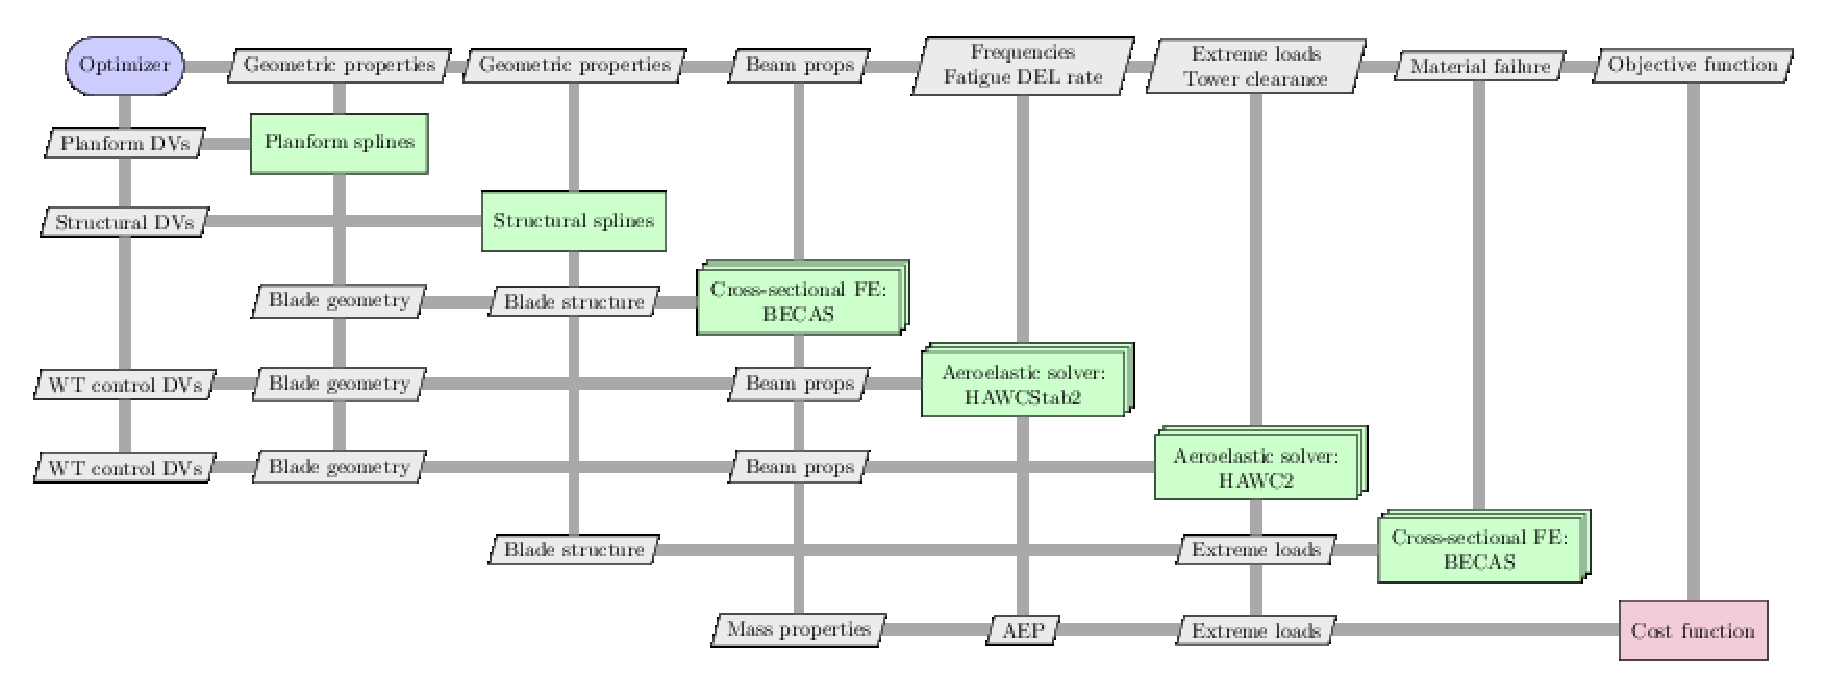
\includegraphics[width=1\linewidth]{figures/hawtopt2_xdsm.eps}
\end{center}
\caption{Extended Design Structure Matrix diagram of the workflow of HawtOpt2.}
\label{fig:xdsm}
\end{figure}


\section{Blade Parametrization}
\label{sec:blade_params}

The blade planform is described in terms of distributions of chord, twist, relative thickness and pitch axis aft leading edge, the latter being the distance between the leading edge and the blade axis.
The lofted shape of the blade is generated based on interpolation of a family of airfoils with different relative thicknesses.

The internal structure is defined from a number of regions that each cover a fraction of the cross-sections along the blade.
Each region consists of a number of materials that are placed according to a certain stacking sequence.
Figure~\ref{fig:cross_section_def} shows a cross section in which the region division points (DPs) are indicated along with the parameterized quantities used to construct the structural geometry.
The composite layup is described by a series of smooth splines describing the thicknesses of individual layers. 
Fore more details on the parametrization see \cite{fusedwind}.

\begin{figure}[!ht]
\begin{center}
        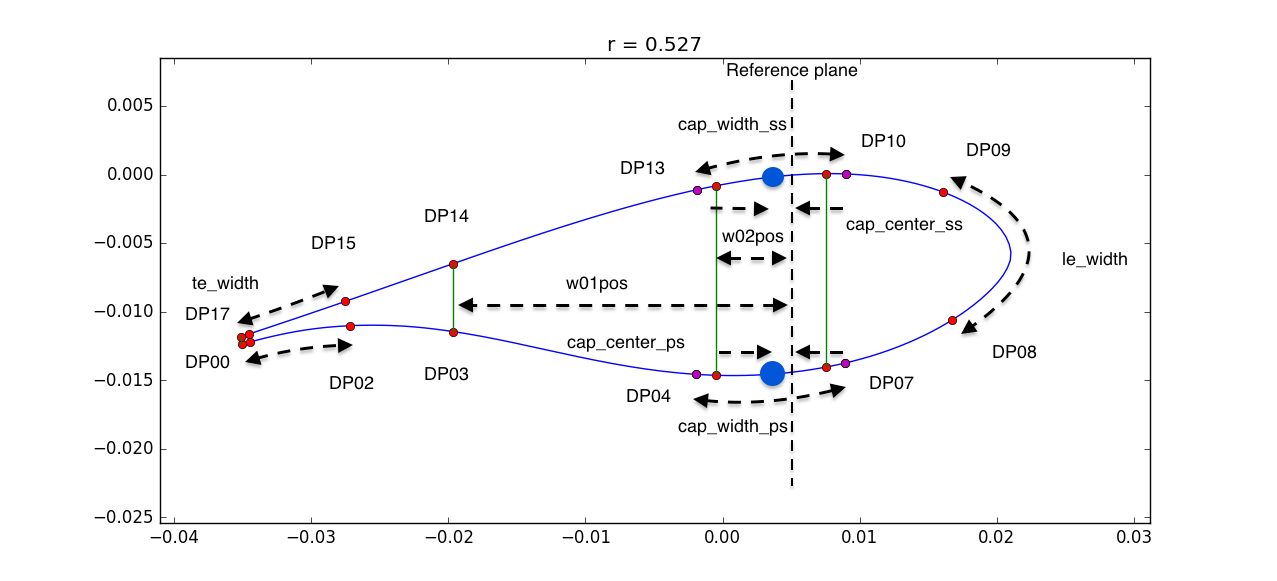
\includegraphics[width=1.\linewidth]{./figures/param2_schematic.eps}
\end{center}
\caption{Region division points (DP) definition: red points indicate division points between regions; their positions are defined as curve fraction from pressure side TE (s=-1) to LE (s=0) to suction side TE (s=1).}
\label{fig:cross_section_def}
\end{figure}

\section{Baseline Design}

The initial data supplied to the project regarding the 100 kW blade consisted of stiffness data as well blade planform, and overall operational characteristics, and component masses.
Data on the airfoils used on the blades or their performance were not supplied.
Neither were details on the internal structure and the materials used.

Several choices had to be made during the initial phases.
In the bullet list below the main choices are listed:

\begin{itemize}

	\item Airfoils: The main airfoil series used is the FFA-W3 series along with a NACA-63-418 tip airfoil.
	\item Airfoil data: Airfoil data was computed using the 2D incompressible CFD solver EllipSys2D \cite{michelsen92,michelsen94,sorensen95}, as a 70/30 blend of clean and tripped flow conditions computed at $Re=1\times10^6$.
	\item Materials: The blade consists of glass fibre only. Materials used are the same as on the DTU 10MW RWT \cite{bakrwt}.
	\item Structural layout: Conventional box structure with linearly tapered main laminates connected with two shear webs.
	\item Blade planform: Based on the externally supplied planform.
\end{itemize}


The following sub-sections describe the steps taken to design the fully described aerostructural blade design for the 100 kW rotor.

\subsection{Airfoil series}

The main airfoil series used is the FFA-W3 series along with a NACA-63-418 tip airfoil.
Figure \ref{fig:baseline_airfoils} shows the 2D cross-sectional shapes of these airfoils.
Figures \ref{fig:baseline_cl} to \ref{fig:baseline_LD} show the lift, drag and lift-to-drag polars of the airfoils computed at a Reynolds number of $Re=1\times10^6$ using EllipSys2D with a mesh consisting of 512 cells in the chordwise direction and 192 cells in the normal direction.
To account for effects of roughness, the polars used were generated from a blend of clean surface, free transition flow and fully turbulent flow, with a blend factor of 0.7/0.3.
360 degree extrapolation of the airfoil data was done using the Viterna method.\footnote{http://wisdem.github.io/AirfoilPreppy/} No 3D correction of the airfoil data was done since the position of the airfoils are changed during optimization, making the 3D correction invalid since it depends on the spanwise position.

\begin{figure}[!ht]
\begin{center}
	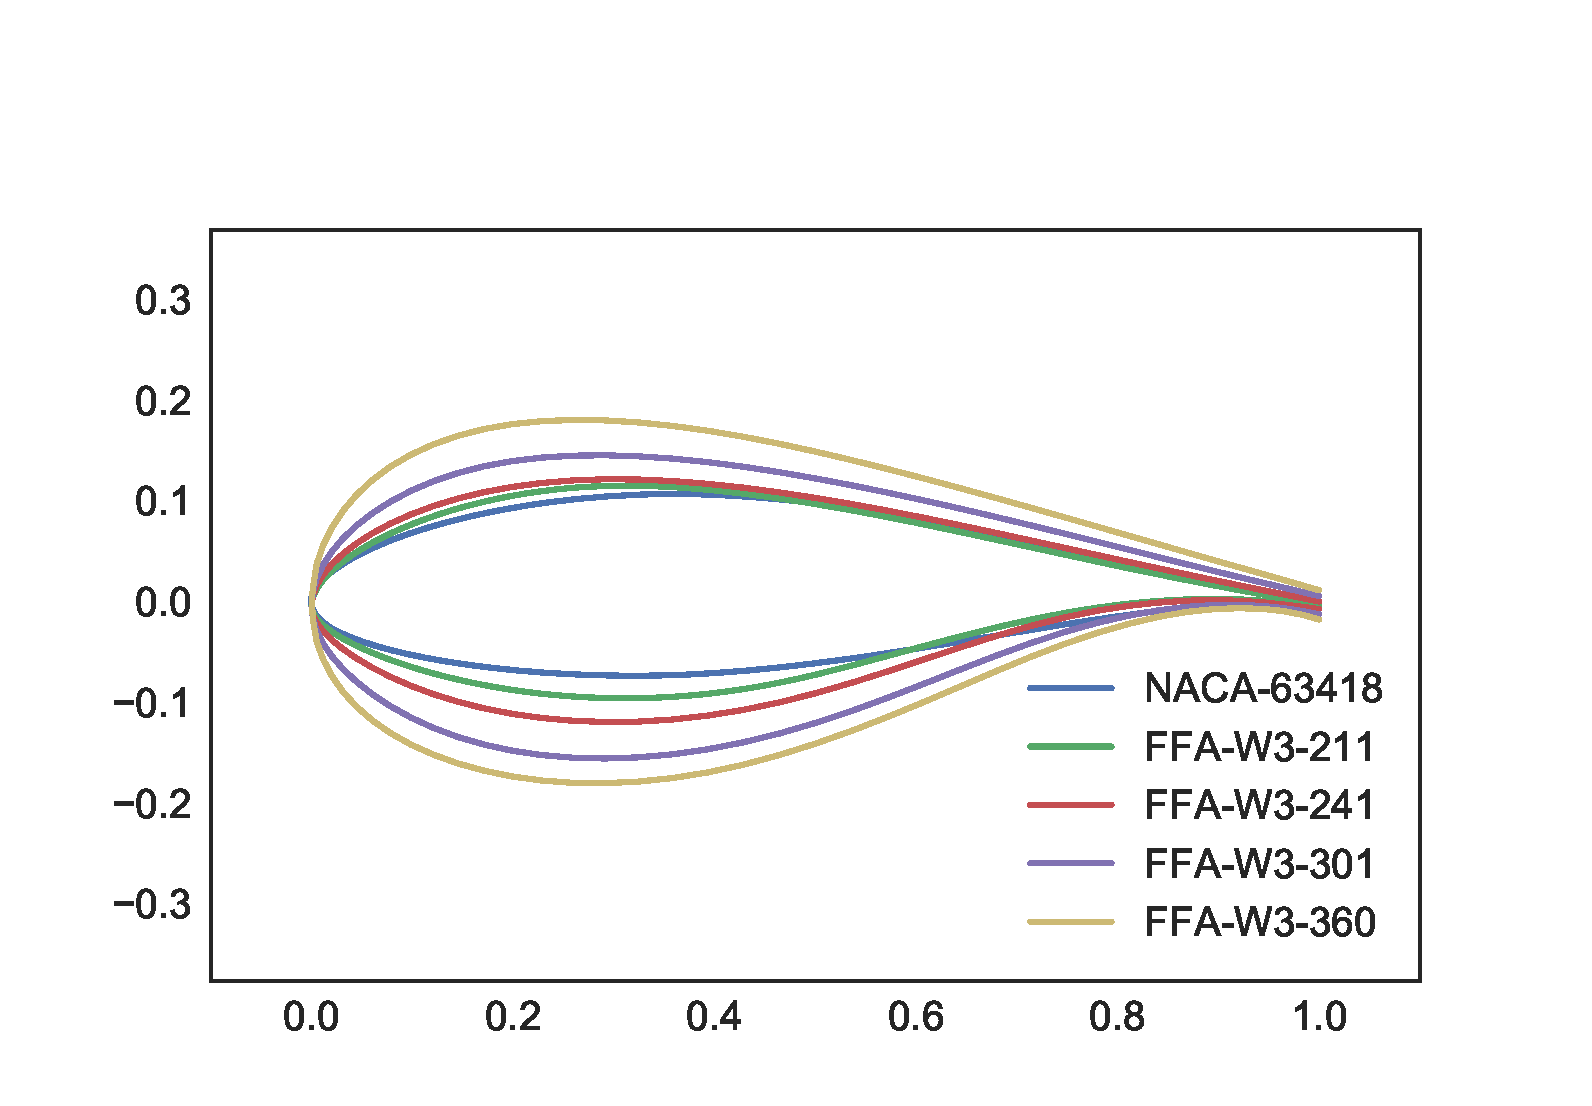
\includegraphics[width=0.8\linewidth]{figures/KB_airfoil_series.eps}
\end{center}
\caption{Airfoils used on the 100kW baseline blade.}
\label{fig:baseline_airfoils}
\end{figure}

\begin{figure}[!ht]
\begin{center}
	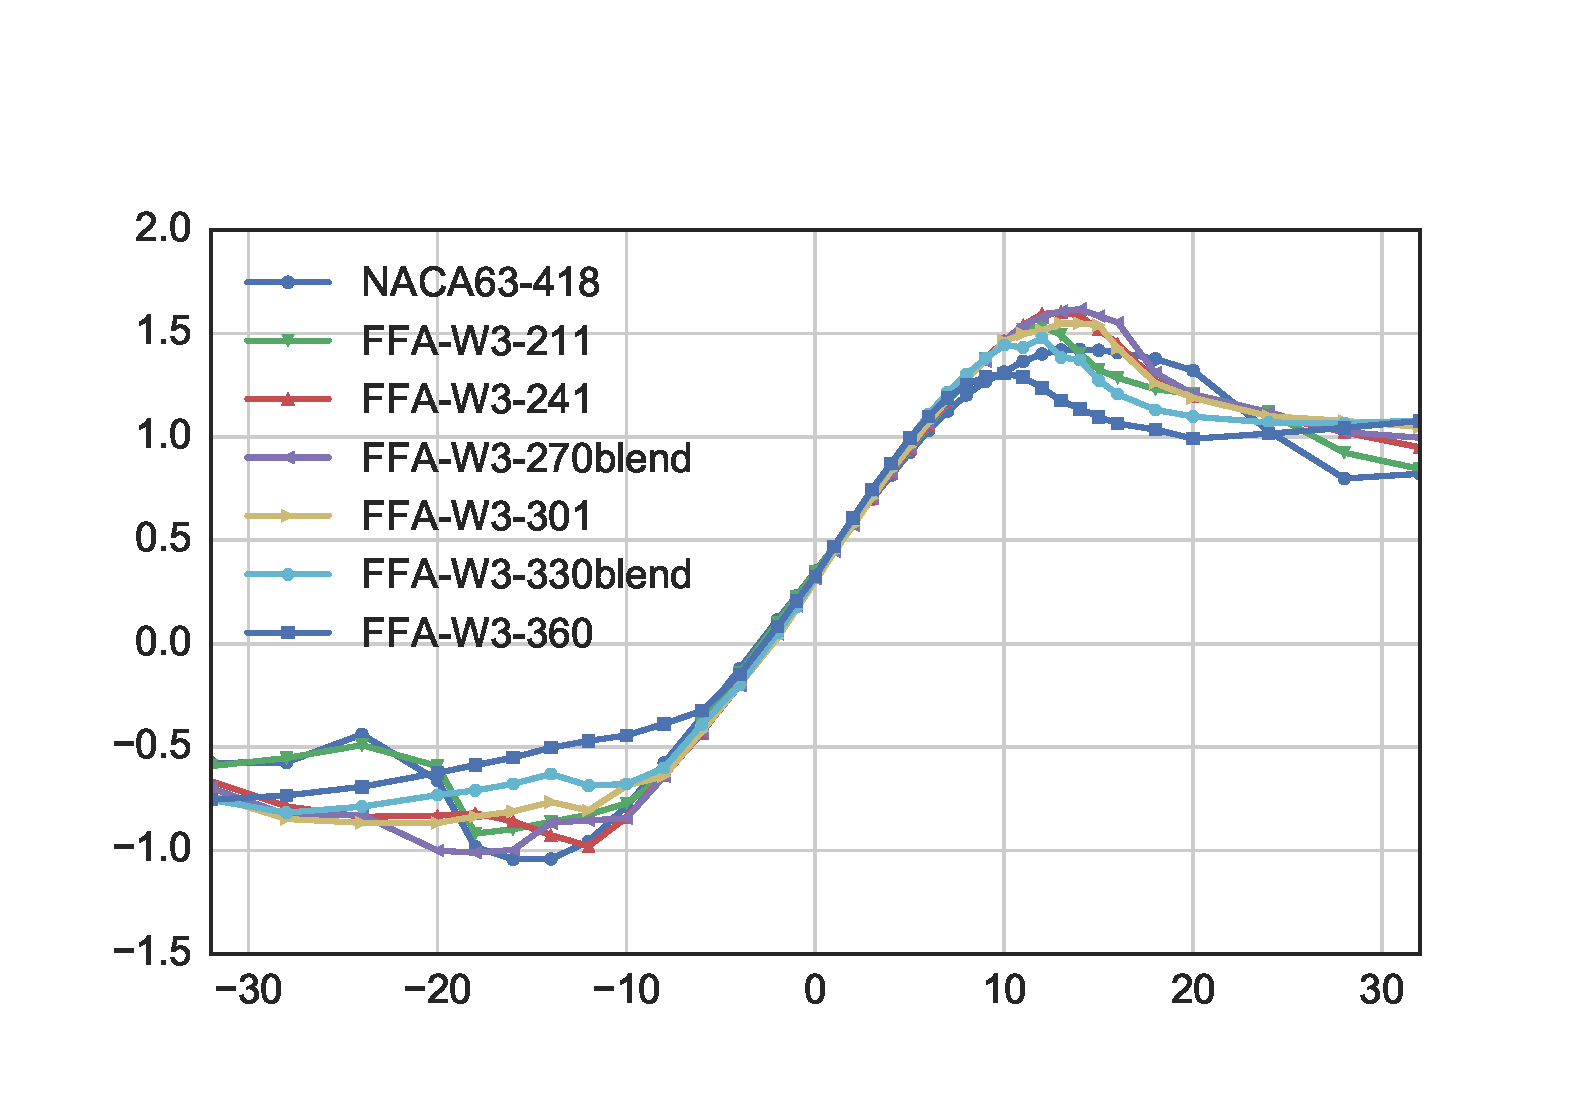
\includegraphics[width=0.8\linewidth]{figures/KB_airfoil_data_cl_detail.eps}
\end{center}
\caption{Airfoil lift coefficients as function of AOA computed at $Re=1e6$.}
\label{fig:baseline_cl}
\end{figure}

\begin{figure}[!ht]
\begin{center}
	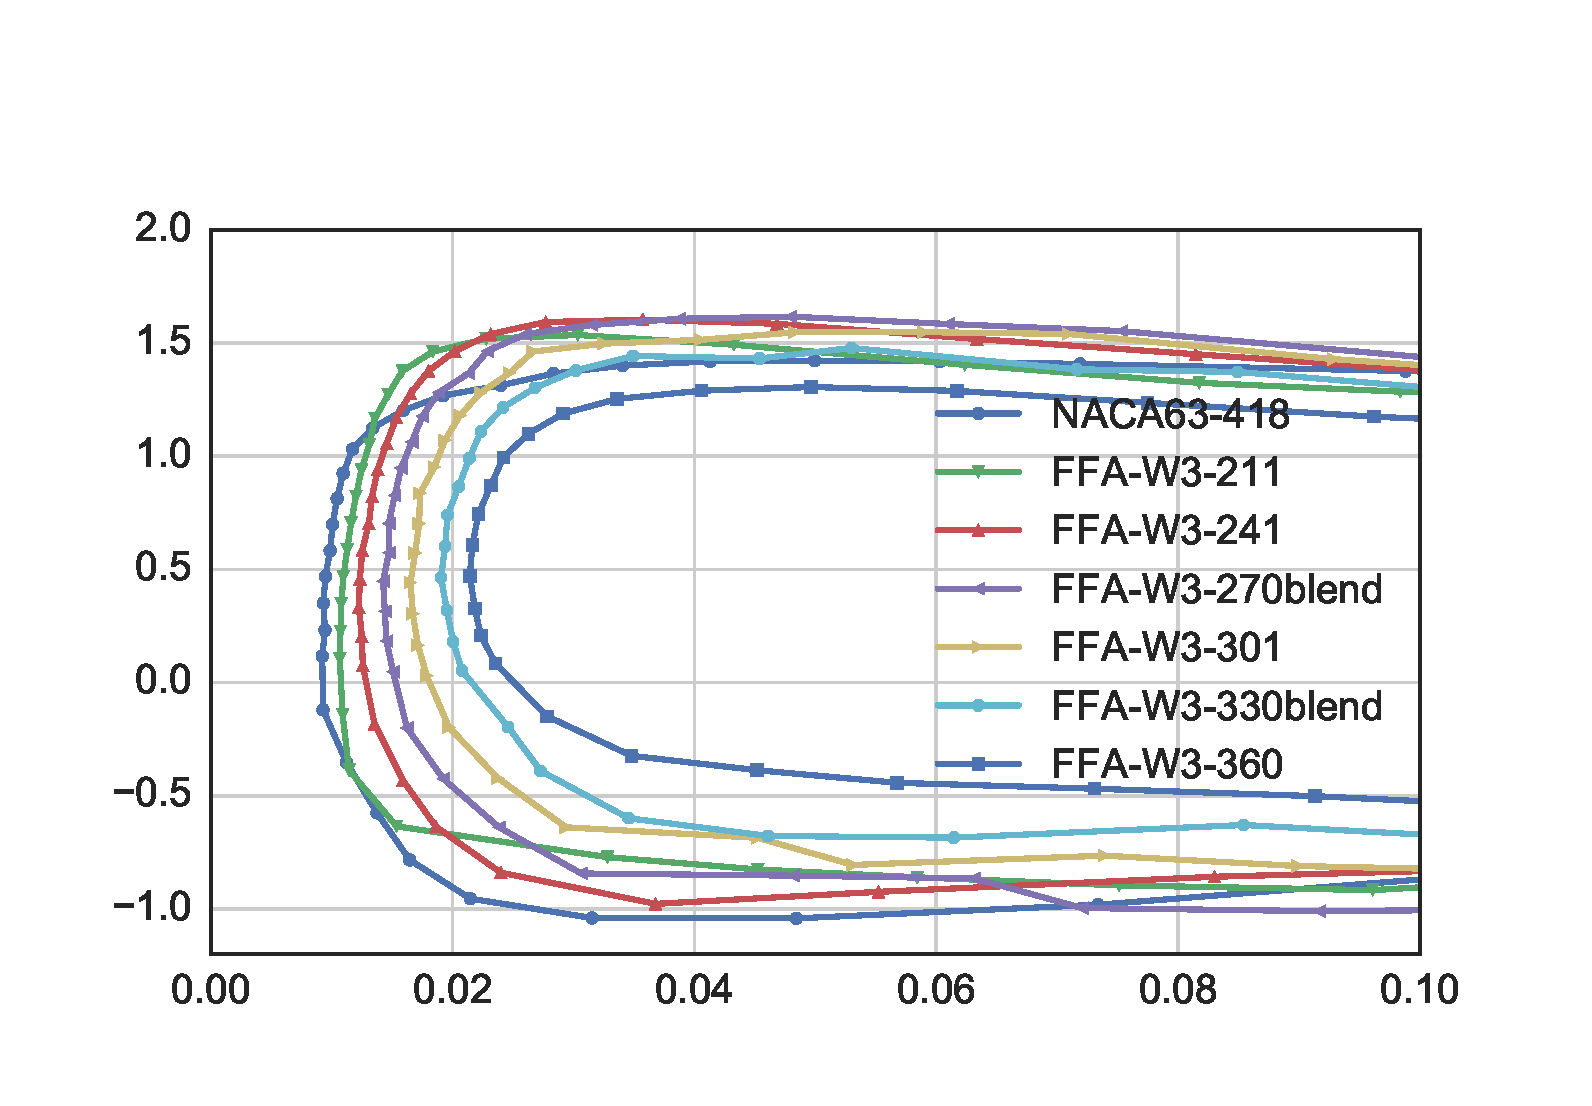
\includegraphics[width=0.8\linewidth]{figures/KB_airfoil_data_cd_detail.eps}
\end{center}
\caption{Airfoil drag coefficients as function of AOA computed at $Re=1e6$.}
\label{fig:baseline_cd}
\end{figure}

\begin{figure}[!ht]
\begin{center}
	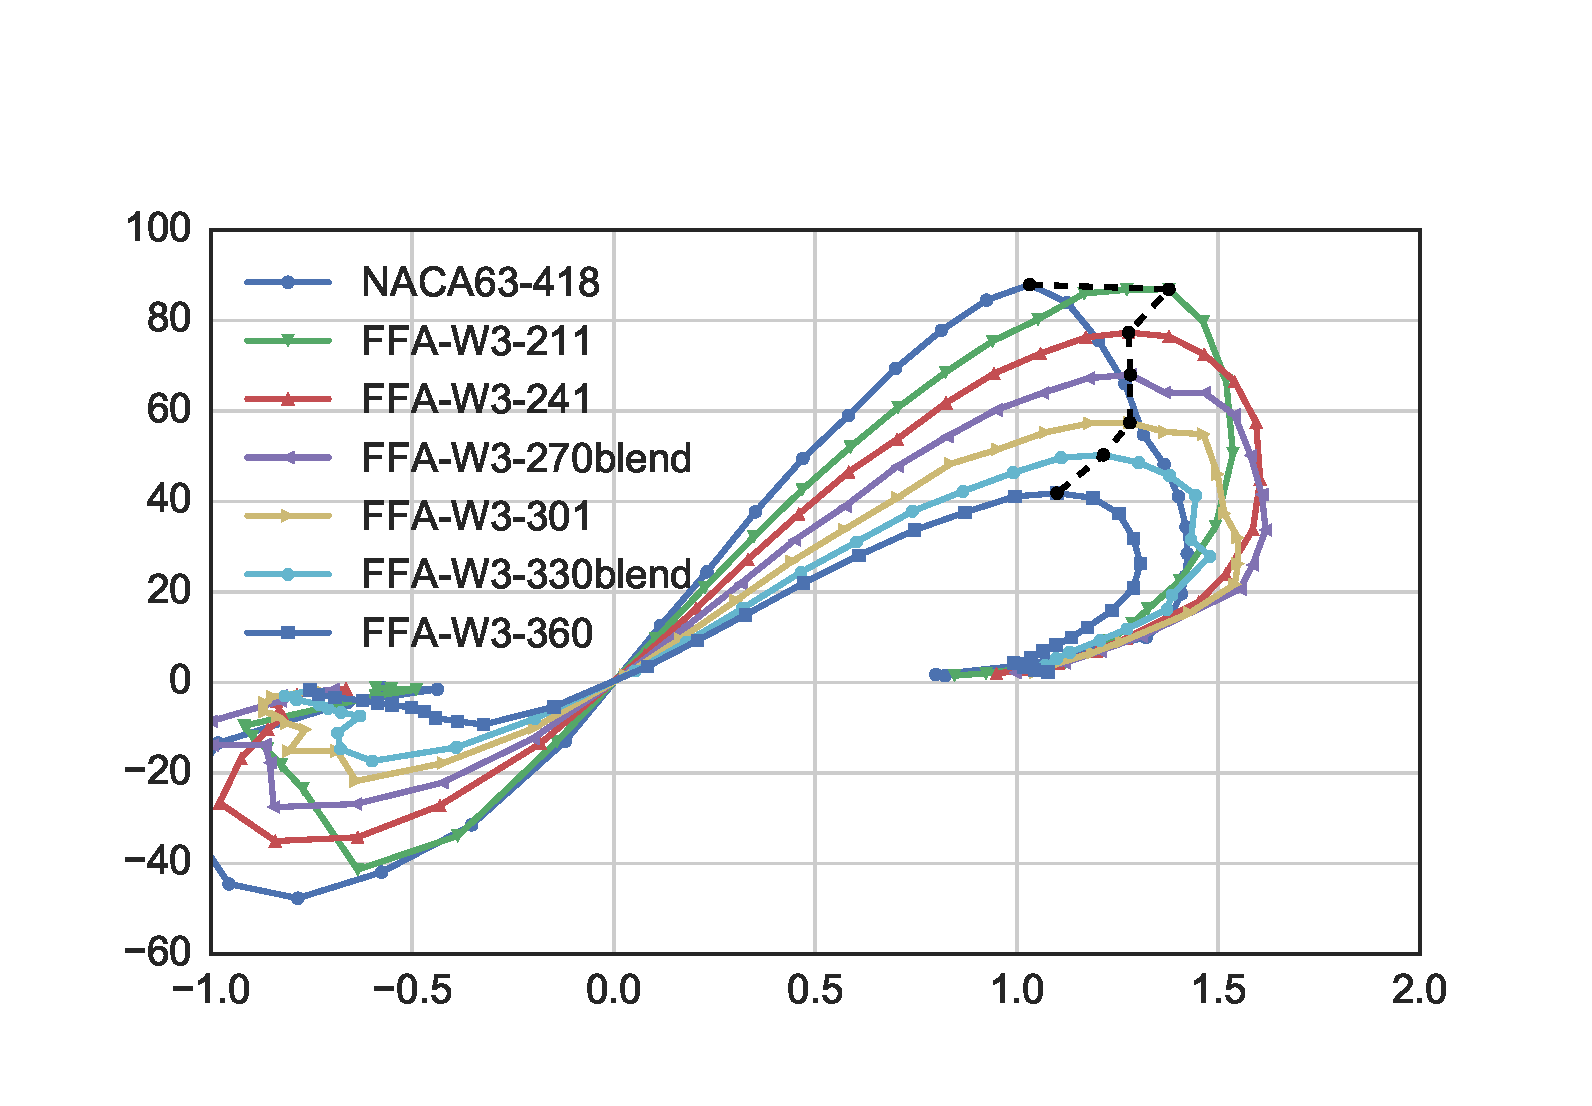
\includegraphics[width=0.8\linewidth]{figures/KB_airfoil_data_clcd_detail.eps}
\end{center}
\caption{Airfoil lift to drag ration as function of $C_l$ computed at $Re=1e6$.}
\label{fig:baseline_LD}
\end{figure}

\clearpage

\subsection{Reference Materials}
\label{sec:reference_mats}

The material properties used for the blade where those defined for the DTU 10 MW RWT (for more details, see \cite{DTU10MW}).
Table \ref{tab:robi_matprop_laminates} lists the apparent mechanical properties of the multidirectional plies used. 

\begin{table}[h!]
\caption{Fiber orientation and apparent mechanical properties of the multidirectional plies.}
\setlength\extrarowheight{2pt}
\centering
\begin{threeparttable}
\begin{tabular}{lcccc}
\hline
Multidirectional Ply    &  \multicolumn{1}{c}{Uniax}  &  \multicolumn{1}{c}{Biax}  & \multicolumn{1}{c}{Triax}  & \tabularnewline
\hline
Fiber volume fraction  $V_\text{f}$   &  0.55  &  0.5  &  0.5  &  -        \tabularnewline
Unidirectional lamina  & \multicolumn{1}{c}{Lamina 2} & \multicolumn{1}{c}{Lamina 1}    & \multicolumn{1}{c}{Lamina 1} & \tabularnewline
\hline
\ang{0} fibers                        &  95    &  0    &  30   & \%  \tabularnewline
\ang{90} fibers                       &  5     &  0    &  0    & \%  \tabularnewline
\ang[retain-explicit-plus]{+45} fibers                       &  0     &  50   &  35   & \%  \tabularnewline
\ang{-45} fibers                      &  0     &  50   &  35   & \%  \tabularnewline
\hline
Young's modulus      $E_1$            &  41.63   & 13.92   &   21.79  & GPa      \tabularnewline
Young's modulus      $E_2$            &  14.93   & 13.92   &   14.67  & GPa      \tabularnewline
Shear modulus     $G_{12}$            &  5.047   & 11.50   &   9.413  & GPa      \tabularnewline
Poisson's ratio $\nu_{12}$            &  0.241   & 0.533   &   0.478  & -        \tabularnewline
Shear modulus $G_{13}=G_{23}$\tnote{(a)} &  5.04698 & 4.53864 &  4.53864 & GPa      \tabularnewline
Mass density        $\rho$            &  1915.5  & 1845.0  &  1845.0  &  $kg/m^3$  \tabularnewline
\hline
\end{tabular}
%\begin{tablenotes}
%\item [(a)] not computed but chosen identical to the values of the respective laminae in Table~\ref{tab:robi_matprop_laminae}.
%\end{tablenotes}
\end{threeparttable}
\label{tab:robi_matprop_laminates}
\end{table}

Design strength properties are also defined for these materials\footnote{Internal communication, provided by Peter Berring} and are listed in Table \ref{tab:matprops_strength} and Table \ref{tab:matprops_strength2}.

\begin{table}[h!]
\caption{Design strength properties of the multidirectional plies.}
\setlength\extrarowheight{2pt}
\centering
\begin{tabular}{lccccccccc}
\hline
\hline
	&$\sigma_{11}^t$ & $\sigma_{22}^t$  & $\sigma_{33}^t$  & $\sigma_{11}^c$  & $\sigma_{22}^c$  & $\sigma_{33}^c$  & $\tau_{12}$   & $\tau_{13}$   & $\tau_{23}$     \\
\hline
Biax	&	69.3         & 69.3  & 69.3  &  64.9 & 64.9  & 64.9  & 55.9 & 55.9 & 55.9 \\
Uniax	&	 360.0         & 24.8  & 24.8  & 257.0 & 63.5  & 63.5  & 16.6 & 16.6 & 16.6  \\
Balsa 	&	 1.0         &  1.0  &  1.0  &   1.0 &  1.0  &  1.0  &  1.0 &  1.0 &  1.0 \\
Triax 	&	186.0         & 30.5  & 30.5  & 152.0 & 51.5  & 51.5  & 42.3 & 42.3 & 42.3 \\
\hline
\hline
\end{tabular}
\label{tab:matprops_strength}
\end{table}


\begin{table}[h!]
\caption{Design strength properties of the multidirectional plies.}
\setlength\extrarowheight{2pt}
\centering
\begin{tabular}{lccccccccc}
\hline
\hline
	&$\epsilon_{11}^t$     & $\epsilon_{22}^t$ & $\epsilon_{33}^t$ & $\epsilon_{11}^c $   & $\epsilon_{22}^c$ & $\epsilon_{33}^t$ & $\gamma_{12}$    & $\gamma_{13} $    & $\gamma_{23}$     \\
\hline
Biax	&	 6.802e-3 & 1.0e6 & 1.0e6 & 7.255e-3 & 1.0e6 & 1.0e6 & 1.0e11 & 1.0e+11 & 1.0e+11 \\
Uniax	&	 6.802e-3 & 1.0e6 & 1.0e6 & 9.523e-3 & 1.0e6 & 1.0e6 & 1.0e11 & 1.0e+11 & 1.0e+11 \\
Balsa 	&	1.000e+6 & 1.0e6 & 1.0e6 & 1.000e+6 & 1.0e6 & 1.0e6 & 1.0e11 & 1.0e+11 & 1.0e+11 \\
Triax 	&	 8.162e-3 & 1.0e6 & 1.0e6 & 9.976e-3 & 1.0e6 & 1.0e6 & 1.0e11 & 1.0e+11 & 1.0e+11 \\
\hline
\hline
\end{tabular}
\label{tab:matprops_strength2}
\end{table}

\clearpage

\subsection{Structural Layout}
\label{sec:sizing}

An approximate sizing of the internal structure was carried out in order to match the stiffness properties supplied from the external partners.
This was done using the BECAS interface in HawtOpt2, where material thickness distributions in 19 cross-sections along the span were sized to match flapwise stiffness, $EI_x$, edgewise stiffness, $EI_y$, and torsional stiffness, $GJ$.
Following this optimization, the material thicknesses were adjusted manually to obtain a reasonably smooth material distribution along the blade.

Table \ref{tab:structure_props} shows the overall properties of the structural geometry. 
The spar cap was tapered from a width of 0.2 m at the root to 0.1 m at the tip, and the trailing edge and leading edge reinforcements had a width of 0.08 and 0.12 m, respectively.
The structural geometry for the blade is plotted in Figure \ref{fig:loftedstructure_baseline_tipview}.

\begin{table}[h!]
\caption{Overall properties of internal structure.}
\centering
\small
\begin{tabular}{{ll}}
\hline
	Spar cap widths	 						& Linear taper 0.2 m (root) to 0.1 m (tip) \\
	Trailing edge panel width upper			& 0.08 m	\\
	Trailing edge panel width lower			& 0.08 m	\\
	Leading edge panel width (upper+lower)	& 0.12 m \\
	Shear web angle relative to rotor plane	& 90 deg	\\
\hline
\end{tabular}
\label{tab:structure_props}
\end{table}


\begin{figure}[pht]
\begin{center}
	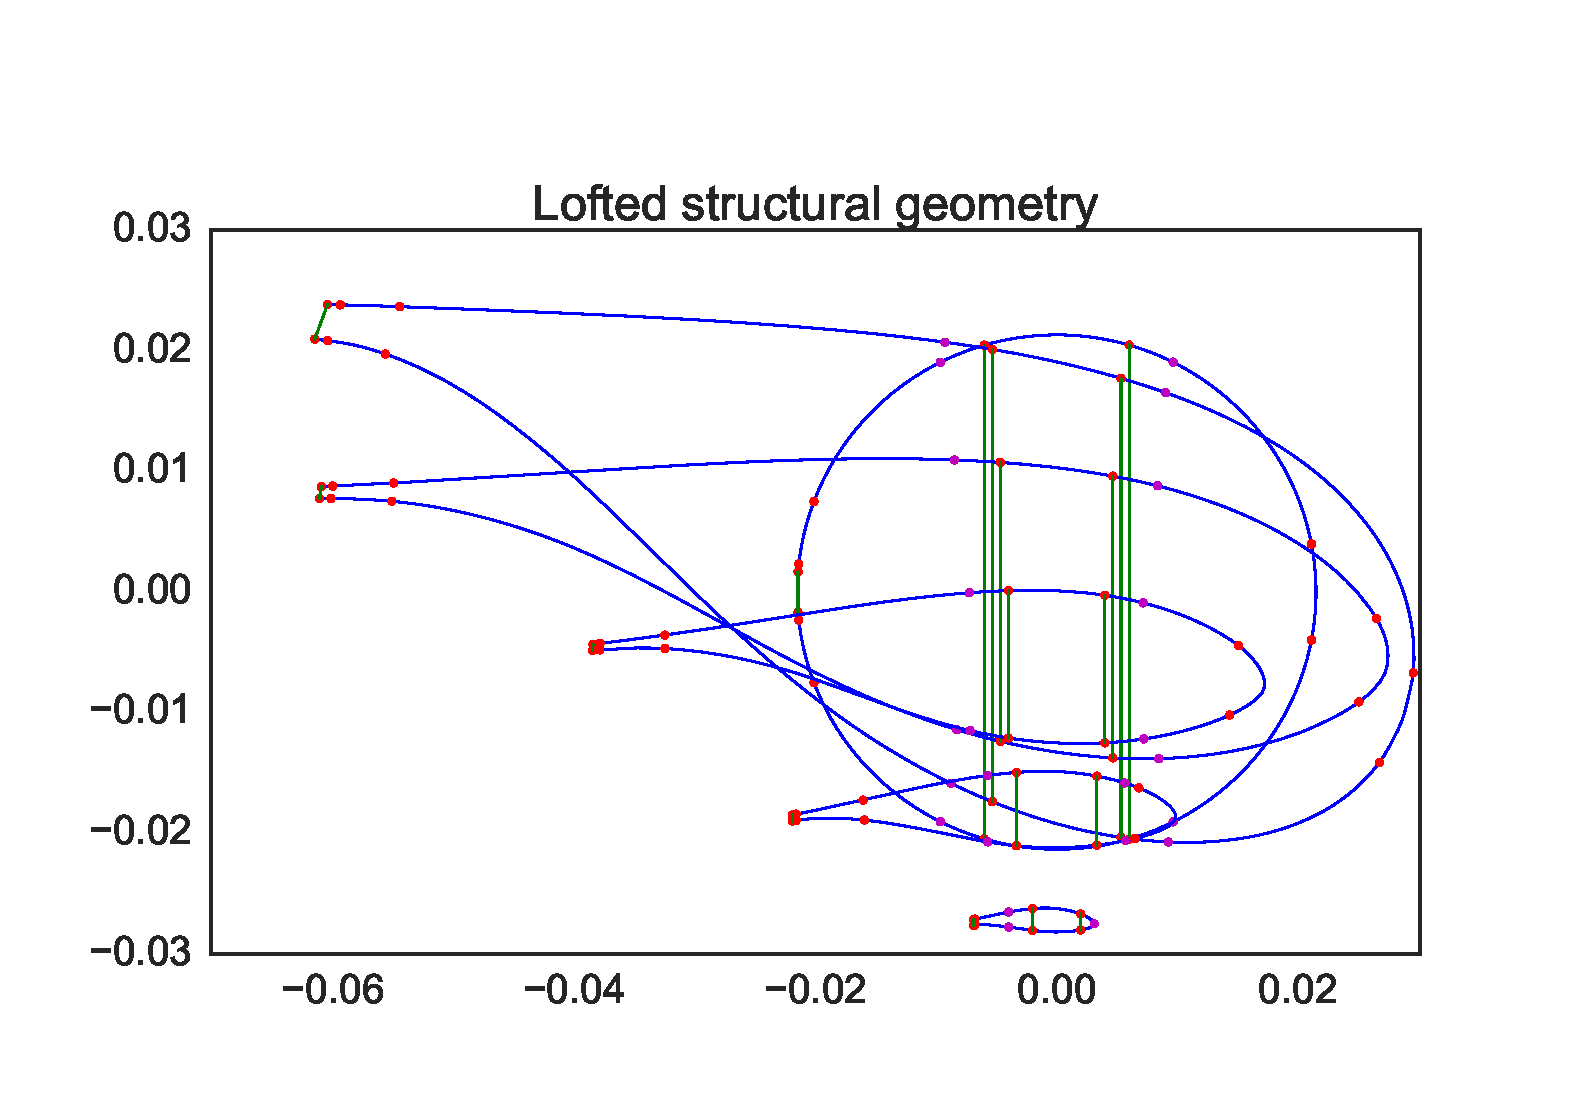
\includegraphics[width=1\linewidth]{figures/baseline_blade_tipview.eps}
\end{center}
\caption{Lofted blade showing internal structural geometry.}
\label{fig:loftedstructure_baseline_tipview}
\end{figure}

Figure \ref{fig:loftedstructure_baseline} shows a 3D plot of the lofted blade structure with material distributions.
%Figure \ref{fig:layups} shows the detailed stacking sequence of materials in the blade.
The total mass of the blade resulting from the sizing process was approximately 230 kg.
This does not include adhesives, surface finishing, and a complete root design.

\begin{figure}[!ht]
\begin{center}
	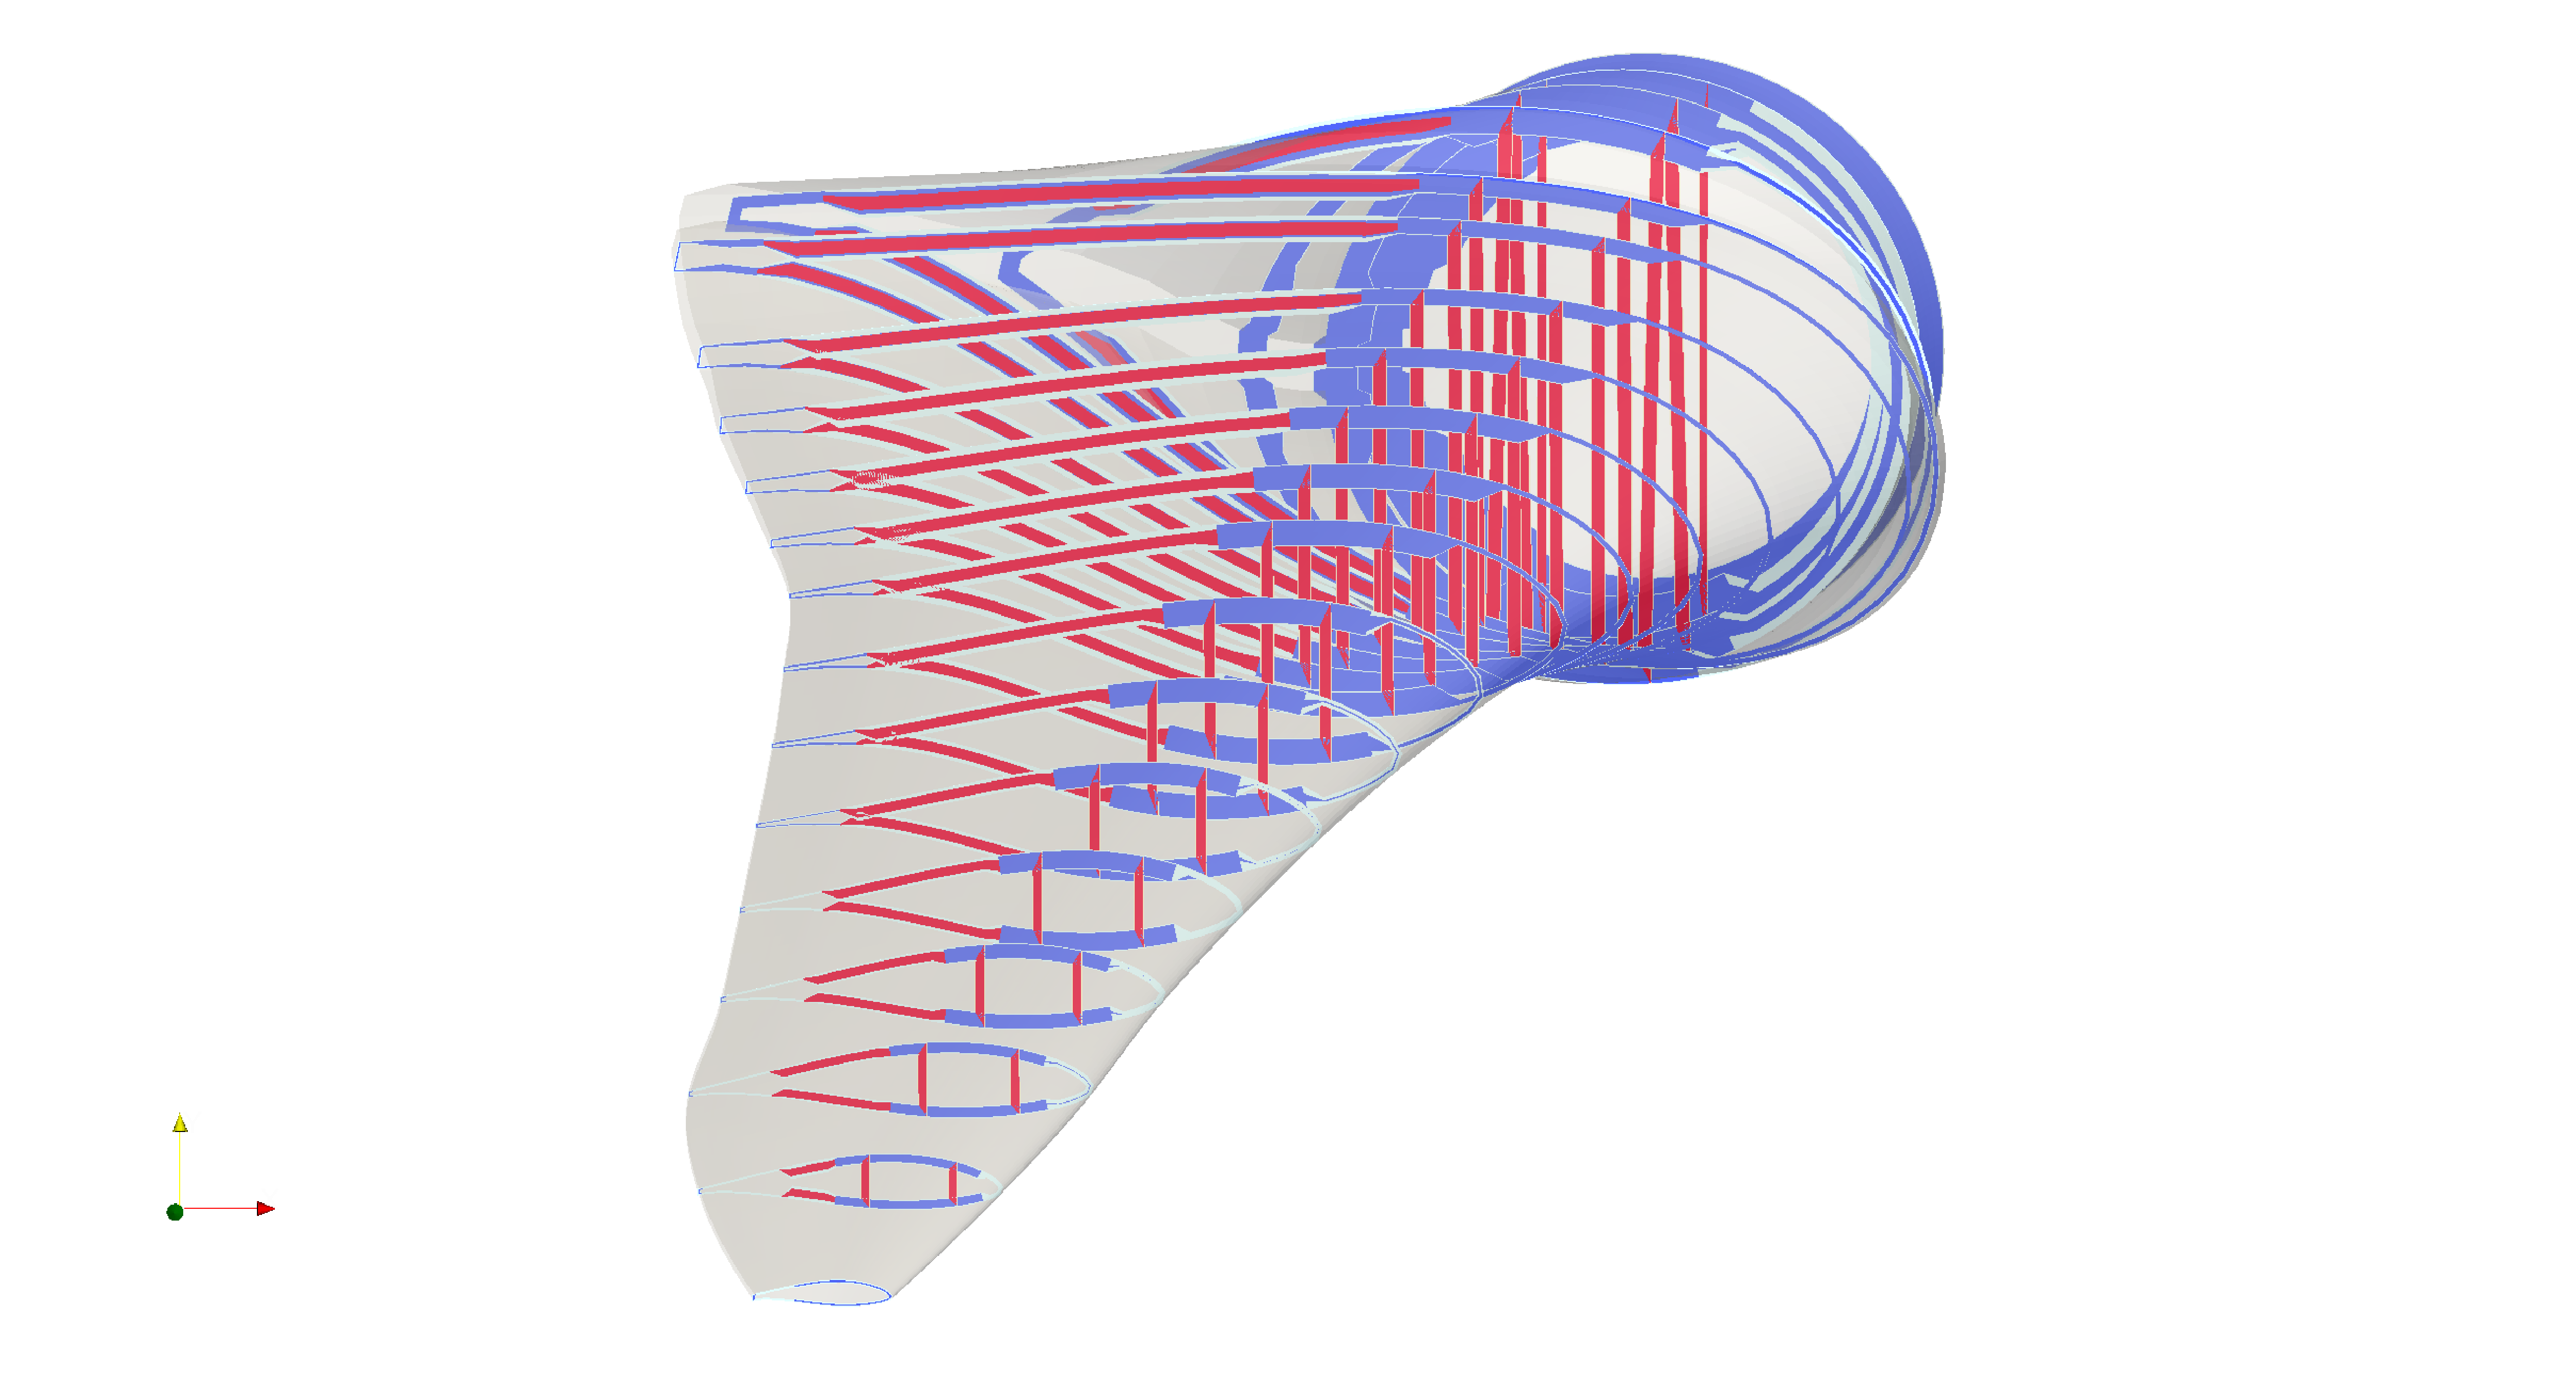
\includegraphics[width=1\linewidth]{figures/loftedbladestructure_basic_sizing.eps}
\end{center}
\caption{Lofted blade showing internal structural geometry.}
\label{fig:loftedstructure_baseline}
\end{figure}

\clearpage
%%------------------------------------------------------------------------------------------------------
%% Start of design compariosions from HAWTOpt2
%%-----------------------------------------------------------------------------------------------------
\section{Design Studies}
\label{sec:design_studies}

In this section five design studies are presented:

\begin{itemize}
	\item \textbf{KB1}: Optimized straight blade. This blade is optimized with constraints on blade torsion to be less than 1 degree at the tip, and no design freedom is given to introduce sweep or material couplings.
	\item \textbf{KB2}: Optimized swept blade. This blade is optimized without constraints on blade torsion and given design freedom to introduce sweep, but not material couplings.
	\item \textbf{KB3}: Optimized material coupled blade. This blade is optimized without constraints on blade torsion and given design freedom to introduce material couplings in the spar cap, but not sweep.
	\item \textbf{KB4}: Optimized swept blade with fixed rotor speed schedule. This blade is optimized without constraints on blade torsion and given design freedom to introduce sweep, but not material couplings. Compared to KB2, additional constraints have been placed on the sweep and prebend. The sweep is constrained to achieve only backward sweep with a maximum limit on its value not exceeding 5\% of the reference blade length. The sweep is only allowed from 60\% blade span and onwards. The prebend too has been constrained to only bend away from the tower with a maximum limit on its value not exceeding 10\% of the reference blade length. An outer layer of triax is added, which is maintained at a fixed thickness through the optimization. The spar cap width is disallowed design freedom. These design decisions have been taken to address manufacturing and structural concerns. Importantly, this design has a fixed rotor speed schedule calculated based on the design tip-speed ratio of the reference blade. 
	\item \textbf{KB6}: Optimized swept blade. This blade is optimized without constraints on blade torsion and given design freedom to introduce sweep, but not material couplings. It incorporates the same design decisions as applied to KB4. However, unlike KB4 the rotor speed schedule is allowed design freedom to vary through the optimization. 
\end{itemize}

All five designs are made with identical optimization problem definitions, that is, same objective and constraints, as well as identical design variables, except for the above mentioned differences. The problem definition is summarized below.

The cost function is defined as
\begin{equation}
f(\{\mathbf{x}_p,\,
	\mathbf{x}_s,\,
	\mathbf{x}_{oper}\},
	\mathbf{p}) = -\frac{AEP(\{\mathbf{x}_p,\,
						  		 \mathbf{x}_s,\,
						  		 \mathbf{x}_{oper}\},
						  		 \mathbf{p})}
						  {AEP(\{\mathbf{0},\,
								\mathbf{0},\,
								\mathbf{0}\},
								\mathbf{p})}	
\label{eqn:objective}
\end{equation}
$AEP$ is the annual energy production and $AEP(\{\mathbf{0},\,\mathbf{0},\mathbf{0}\}, \mathbf{p})$ is the annual energy production of the baseline design.
Three different types of constraints are defined depending on the variables they depend on. 
Constraints $\mathbf{g}$ depend only on planform parameters. 
They include bounds on the chord and relative thickness. 
Constraints $\mathbf{h_g}$ depends only on structural parameters.
These constraints include bounds on the material thicknesses and on the position and widths of the spar caps. 
Constraints $\mathbf{h_s}$ denote the limits on the maximum allowable stresses in the structure.
The constraints $\mathbf{k}$ depend on both the planform and structural variables, such as blade tip deflection and loads.

Tables \ref{tab:dv_summary} and \ref{tab:con_summary} provides a summary of design variables and constraints used in this study.

\begin{table}[pth]
\centering
\caption{Free form deformation spline (FFD) design variables used in the optimizations.}
\small
\begin{tabular}{p{5cm}lp{6cm}}
\hline
\textbf{Parameter}		&	\# of DVs			& \textbf{Comment}	\\
\hline
Chord					&	6	&	-	\\
Twist					&	5	&	Root twist fixed	\\
Relative thickness		&	4	& 	Root and tip relative thickness fixed	\\
Out of plane prebend		&	3	& 	- \\
In-plane sweep			&	4	&	Active for KB2, KB4 and KB6 design \\
Pitch axis aft LE		&	4	& 	- \\
Blade length				&	1	&	- \\
Tip-speed ratio			&	1	&	Inactive in KB4 to ensure fixed RPM schedule. \\
Trailing edge uniax		&	4	&	Symmetric pressure/suction side	\\
Spar cap uniax			&	4	&	Symmetric pressure/suction side	\\
Leading edge uniax		&	4	&	Symmetric pressure/suction side	\\
Leading panels triax		&	4	&	Symmetric pressure/suction side	\\
Trailing panels triax	&	4	&	Symmetric pressure/suction side	\\
Spar cap width			& 	2	&	Linearly tapered spar cap. Inactive in KB4 and KB6. \\
Suction side spar cap fibre angle	&	4	&	Only active for KB3 design	\\
Pressure side spar cap fibre angle	&	4	&	Only active for KB3 design	\\
\hline
\textbf{KB1 Total}		&	44	&	\\
\textbf{KB2 Total}		&	48	&	\\
\textbf{KB3 Total}		&	52	&	\\
\textbf{KB4 Total}		&	48	&	\\
\textbf{KB6 Total}		&	49	&	\\
\hline
\end{tabular}
\label{tab:dv_summary}
\end{table}

\begin{table}[pth]
\centering
\caption{Non-linear constraints used in the design process.}
\small
\resizebox{\linewidth}{!}{
\begin{tabular}{p{4.5cm}lp{6cm}}
\hline
\textbf{Constraint}					&	Value			& \textbf{Comment}	\\
\hline
max(chord)							&	$< 0.9$	m		&	Maximum chord limited for transport.	\\
max(prebend)							&$<0.9$ m (for KB1,KB2, KB3) 		&	Maximum prebend limited for transport.	\\
                                   &   $< 1$ m (for KB4 and KB6)	  &                                                     \\
max(sweep)							& $< 0.9$ m (for KB2)			& Maximum sweep limited for ease in manufacturing.	\\
                                   &   $< 0.5$ m (for KB4 and KB6)  &                                                     \\
min(relative thickness)				&	$> 0.18$			&	Fixed airfoil series.	\\
min(material thickness)				&	$> 0.0 $ m		&	Allow maximum freedom to reduce thickness - although unrealistic.	\\
max(Blade deflection)				&	$< 1.0$ m		&  	Allow blade tip to deflect 1 m.\\
Blade root flapwise moments (MxBR\_steady)	&	$<$ ref value	&  	Steady state loads cannot exceed starting point.\\
Rotor thrust (T\_steady)				&	$<$ ref value	&  	Steady state loads cannot exceed starting point.\\
Blade root flapwise moments (MxBR)	&	$<$ ref value	&  	Reduced DLB loads cannot exceed starting point.\\
Blade root edgewise moments (MyBR)	&	$<$ ref value	&  	Reduced DLB loads cannot exceed starting point.\\
Blade root pitch moments (MzBR)		&	$<$ ref value	&  	Reduced DLB loads cannot exceed starting point.\\
Tower top thrust (FyTT)				&	$<$ ref value	&  	Reduced DLB loads cannot exceed starting point.\\
Tower bottom fore-aft moment (MxTB)				&	$<$ ref value	&  	Reduced DLB loads cannot exceed starting point.\\
Rotor torque							&	$<$ ref value	&  	Ensure that the rotational speed is high enough below rated to not exceed generator maximum torque.\\
Blade mass							&	$<$ 1.01 * ref value	&  	Limit increase in blade mass to maintain equivalent production costs.\\
Blade mass moment					&	$<$ 1.01 * ref value	&  	Limit increase in blade mass moment to minimise edgewise fatigue.\\
Lift coefficient @ $r/R=[0.5-1.]$	&	$<$ 1.4-1.1			&	Limit operational lift coefficient to avoid stall for turbulent inflow conditions.\\	
\hline
\end{tabular}}
\label{tab:con_summary}
\end{table}

\subsection{Overview of the designs}
\label{subsec:design_overview}
The overall properties of the five optimized blades and the reference design are listed in Table \ref{tab:overall_summary}, along with their relative changes with respect to the reference blade.
Both KB2 and KB3 produce higher AEP than the non-coupled KB1 blade, and we also see that swept KB2 blade performs better than the material coupled design KB3. The increased performance of KB2 is also reflected in the slightly longer blade length of 11.35 m, compared to 11.064 and 11.231 of KB1 and KB3.


As mentioned at the beginning of Section \ref{sec:design_studies}, the KB4 and KB6 designs have additional constraints placed on the magnitude of sweep and prebend, along with reduced freedom provided to the optimizer in changing the material thicknesses in the laminae. These factors influence the design resulting in lower AEP compared to the non-coupled blade KB1. For instance, a lower limit on backward sweep prevents additional load reduction benefits through the phenomenon of geometric bend-twist coupling. A lower load reduction potential in turn limits the achievable blade length, which is a major driver of aerodynamic loads. This is seen in the lower blade length values obtained by KB4 and KB6 compared to the three remaining designs. Additionally, KB4 follows a fixed rotor speed schedule based on the tip speed ratio of the reference blade. As a result the KB4, rotor operates at the same rotor speeds as the reference rotor for given wind speeds. This limits the achievable AEP increase as the blade fails to operate at its optimal aerodynamic design points. The influence of the design freedom assigned to rotor speed is seen in the superior AEP of KB6 over that of KB4. This is achieved inspite of only a slight increase of blade length in KB6, pointing to the influential role of rotor speed to facilitate optimal operation of the rotor in the variable speed region.

All blades operate at high tip speed ratio, compared to the starting point of the design optimizations of 7.5. Since the blade mass was a constraint in the optimizations, all five blades have similar mass with KB6 being the heaviest.

%\begin{table}
%\begin{tabular}{l|l|l|l|l|l|l}
%\hline
% Quantity              & Reference & KB1 & KB2     & KB3     & KB4    & KB6          \\
%\hline
% AEP [MWhr] (A=6, k=2) & 212.38 & 243.82 & 252.18  & 249.08  & 224.67 & 236.77  \\
% Blade length [m]      & 10.00  & 11.06  & 11.41   & 11.22   & 10.48  & 10.55  \\
% blade\_mass [kg]      & 273.16 & 256.87 & 257.71  & 256.65  & 254.53 & 260.46 \\
% TSR [-]               & 7.50   & 10.08  & 10.625  &  9.779  & 7.68   & 9.77 \\
%\hline
%\hline
%\end{tabular}
%\caption{Summary of overall properties of the five optimized blades.}
%\label{tab:overall_summary}
%\end{table}

%\begin{table}
%\begin{tabular}{l|l|l|l|l|l|l}
%\hline
% Quantity             &  KB1 & KB2     & KB3     & KB4    & KB6          \\
%\hline
% AEP (A=6, k=2)  & +14.80\%  & +18.74\%  & +17.28\%   & +5.79\%   &  +11.48\% \\
% Blade length    &  +10.6\% & +14.1\%   & +12.2\%   &  +4.8\%  & +5.5\%  \\
% blade\_mass      & -5.96\% & -5.66\%  & -6.04\%  & -6.82\% &  -4.65\%\\
% TSR             & +34.4\%  & +41.67\%  &  +30.39\%  & +2.4\%   & +30.27\% \\
%\hline
%\hline
%\end{tabular}
%\caption{Summary of relative change of overall properties of the five optimized designs with respect to the reference blade.}
%\label{tab:overall_summary}
%\end{table}

\begin{table}[pht]
\centering
\caption{Summary of overall properties of the five optimized blades.}
\label{tab:overall_summary}
\resizebox{\linewidth}{!}{
\begin{tabular}{|l|l||l|l||l|l||l|l||l|l||l|l|}
\hline
\multirow{2}{*}{Quantity}                         & Reference & \multicolumn{2}{l||}{KB1} & \multicolumn{2}{l||}{KB2} & \multicolumn{2}{l||}{KB3} & \multicolumn{2}{l||}{KB4} & \multicolumn{2}{l|}{KB6} \\ \cline{2-12}
                 & Value     & Value      & Change     & Value      & Change     & Value      & Change     & Value      & Change     & Value      & Change     \\\hline
AEP{[}MWhr{]} (A=6, k=2) & 212.38    & 243.82     &  +14.80\%          & 252.18     &   +18.74\%         & 249.08     &   +17.28\%         & 224.67     &       +5.79\%     & 236.77     &    +11.48\%        \\ 
Blade length {[}m{]}     & 10        & 11.06      &   +10.6\%         & 11.41      &    +14.1\%         & 11.22      &   +12.2\%         & 10.48      &        +4.8\%     & 10.55      &  +5.5\%          \\ 
Blade mass {[}kg{]}     & 273.16    & 256.87     &   -5.96\%         & 257.71     &    -5.66\%        & 256.65     &    -6.04\%         & 254.53     &        -6.82\%    & 260.46     &       -4.65\%     \\ 
TSR {[}-{]}              & 7.50      & 10.08      &    +34.4\%        & 10.62      &   +41.67\%         & 9.78       &    +30.39\%         & 7.68       &      +2.4\%      & 9.77       &     +30.27\%  \\ \hline    
\end{tabular}}
\end{table}
The differences in the AEP of the five optimized designs and the reference rotor is represented visually in Figure \ref{fig:KB_AEP}. The AEPs have been calculated for a Weibull wind climate with average wind speed of 6 m/s.
Figures \ref{fig:power} to \ref{fig:rpm} show the rotor steady state performance as function of wind speed. The mechanical power generated by the optimized designs is shown in Figure \ref{fig:power}. It is seen that the only KB4 and the reference blade achieve rated power at a wind speed of 11 m/s whereas the rest of the designs produce rated power at a wind speed of 10 m/s. This due to a shorter variable speed region in KB1, KB2, KB3 and KB6 as a result of the rotor speed being granted design freedom during the optimization. In general, KB4 and reference produce similar power for a given wind speed and is lower than the rest of the designs. This is due to the higher rotor speeds adopted in these designs than compared to KB4, which follows the same rotor speed schedule as the reference. A higher optimal rotor speed results in a higher optimal tip-speed ratio. The rotor speed curves can be seen in Figure \ref{fig:rpm}. All the designs except for KB4 and the reference attain the rated rotor speed of 70 rpm between 8 and 9 m/s, whereas KB4 and the reference rotor attain the maximum rotor speed between a wind speed of 10 and 11 m/s. 

The power coefficient curves shown in Figure \ref{fig:cp} are seen to decrease in the bend-twist coupled designs with increasing loading due to increase in wind speeds. This is especially true in the KB2 swept blade, where the high magnitude of sweep causes a high value of torsion towards feather decreasing the angle of attack from the design point resulting in a decreased lift coefficient and hence a reduced power coefficient. Due to additional constraints on the maximum attainable sweep placed in the KB6 swept blade design, the decrease in the effective angle of attack caused by increasing magnitudes of torsion with rising wind speeds is not large enough to cause the blade sections to operate outside the optimal aerodynamic region. Thus, the power coefficient remains constant until the rated rotor speed is achieved, beyond which a decrease in the tip-speed ratio causes the observed decrease in the power coefficient. The same trend in the power coefficient is also observed in the KB1 non-coupled blade where there is no bend-twist coupling phenomenon affecting the performance. However, the bend-twist coupled blades show a reduction in the thrust coefficient with increasing wind speeds due to the corresponding rise in magnitudes of torsion towards feather. This can be observed in the thrust coefficient curves shown in Figure \ref{fig:ct}. It is noted that the rate of decrease in the power coefficient of the coupled designs is lower than the corresponding rates of decrease in the thrust coefficient, highlighting the effectiveness of bend-twist coupling towards feather as a load reduction method. Beyond the attainment of the rated rotor speed a decrease in thrust coefficient is also observed in the non-coupled KB1 blade along with the coupled designs. The high tip speed ratio (TSR) operation causes the constant TSR region to end between 8 and 9 m/s, as they attain the rated rotor speed. Beyond this point the decreasing TSR with rising wind speed results in a reduction in $C_T$, which has a beneficial effect on also tip deflection resulting in an unloaded blade tip region. This is a common feature in all the optimized blades apart from KB4, where the decrease in the thrust coefficient is primarily due to bend-twist coupling.         

The thrust curves of the five designs are shown in Figure \ref{fig:thrust}. Here too the designs operating at higher rotor speeds and corresponding high tip-speed ratios have a greater magnitude of thrust than KB4 and reference blades for the same wind speeds. They attain peak thrust corresponding to maximum rotor speed at a wind speed between 8 and 9 m/s, lower than that of KB4. Furthermore, the peak thrusts for the swept blade designs of KB2, KB4 and KB6 are seen to not exceed the peak thrust in the reference case. The peak thrust in KB1 and KB3 are marginally higher than the reference case but within the acceptable deviation of 7\%.

Finally, the pitch curve of the optimized designs is shown in Figure \ref{fig:pitch}. The blade is not pitched until it reaches the rated rotor speed, beyond which the blades are pitched to curtail loads and power.

Figure \ref{fig:powerratio} depicts the ratio of the power produced in the optimized rotors to that of the reference rotor. It is seen that the KB2 swept blade significantly outperforms the rest of the design with regards to this metric. The KB3 blade is seen to produce more than the rated power for the region above the rated wind speed.  
It should be noted that the extra power being produced in the KB3 design stems from the difference in the tool used for its aeroelastic evaluation compared to the rest of the blades. KB3, being a material coupled design, had to be evaluated using the time domain aero-servo-elastic tool HAWC2, whereas the rest of the designs were evaluated with the HAWCStab2 aeroelastic solver. This was required as HAWCStab2 currently lacks the functionality to evaluate material coupled designs. Being a time domain tool, HAWC2 requires a tuned controller to curtail the power output to rated, for the region above the rated wind speed. The need to tune the controller arises with a change in the rotor design. The optimization framework provided by HawtOpt2 currently lacks the capability to tune the controller for the constant speed region above the rated wind speed. Thus, KB3 operates with the tuning parameters from the reference blade. The influence of the performance of the turbine in the region above the rated wind speed is minimal on the optimization and the resulting final design. Since this region is pitch controlled, the loads will not exceed those experienced in the variable speed region. The load reduction in the variable speed is one of the main design drivers in the aeroelastically tailored blade for a pitch regulated variable speed turbine. Additionally, the high wind speeds encountered above rated have a low chance of occurrence for the given wind climate. Finally, it was decided to proceed with a swept blade design and hence additional resources were not spent in the tuning of the controller and revaluation of the KB3 design with the tuned controller, especially since it is not expected to result in a significant difference over the current design.


\begin{figure}[pht]
\begin{center}
	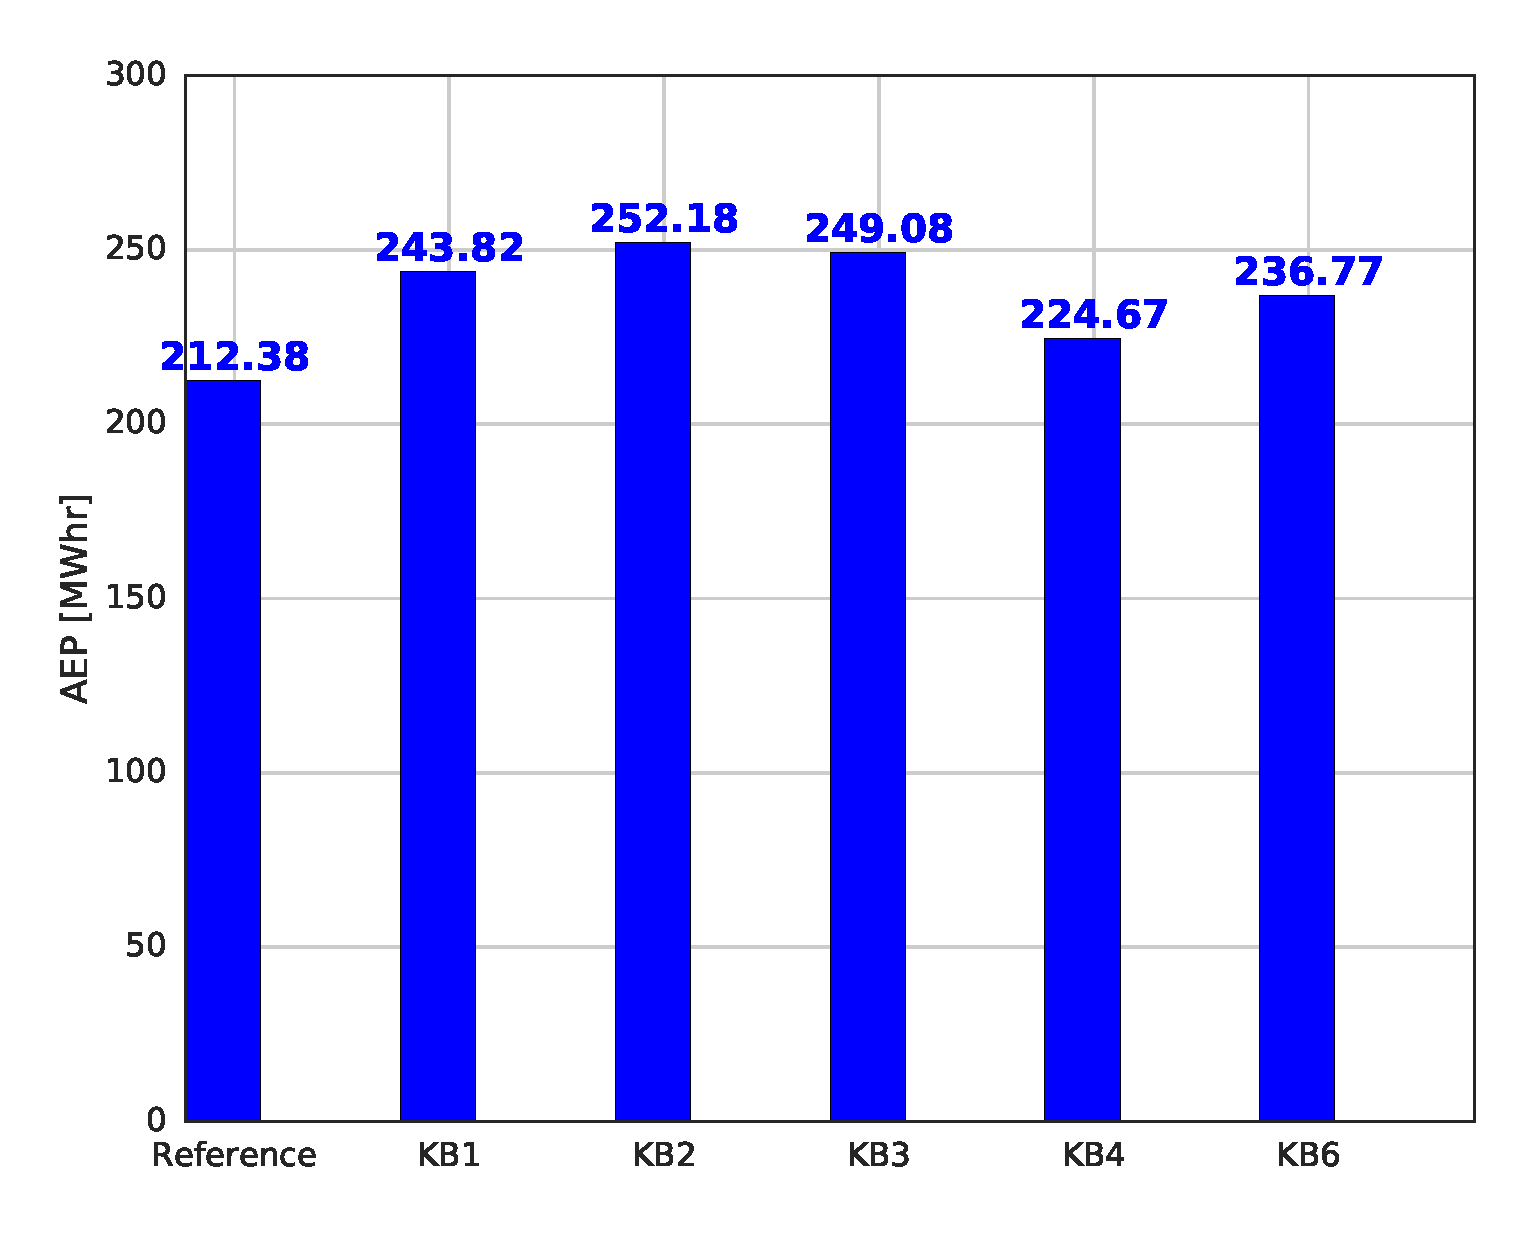
\includegraphics[width=.85\linewidth]{figures/KBcomp_AEPcomp.eps}
\end{center}
\caption{Annual energy production of the five optimized blades for a Weibull wind distribution with scale factor A=6.0 m/s and shape factor k= 2.0 [-].}
\label{fig:KB_AEP}
\end{figure}

\begin{figure}[pht]
\begin{center}
	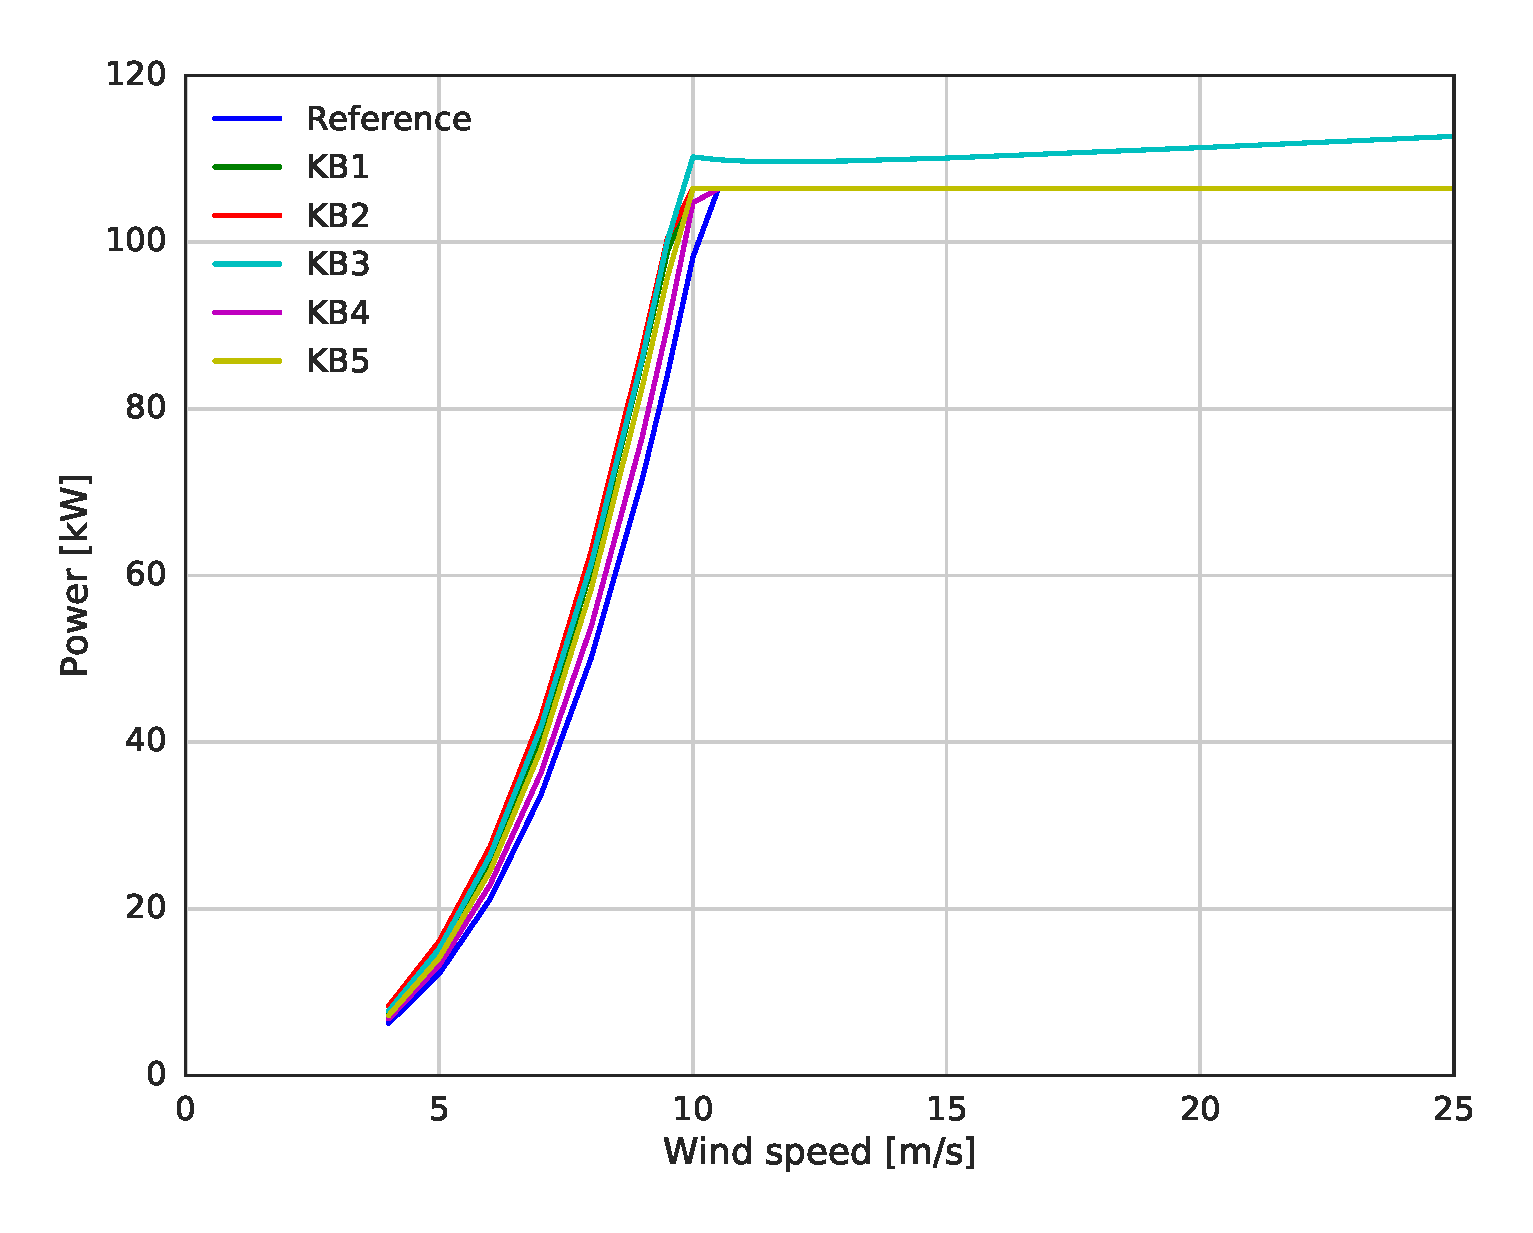
\includegraphics[width=.85\linewidth]{figures/KBcomp_power.eps}
\end{center}
\caption{Mechanical power as function of wind speed for the five optimized blades.}
\label{fig:power}
\end{figure}

\begin{figure}[pht]
\begin{center}
	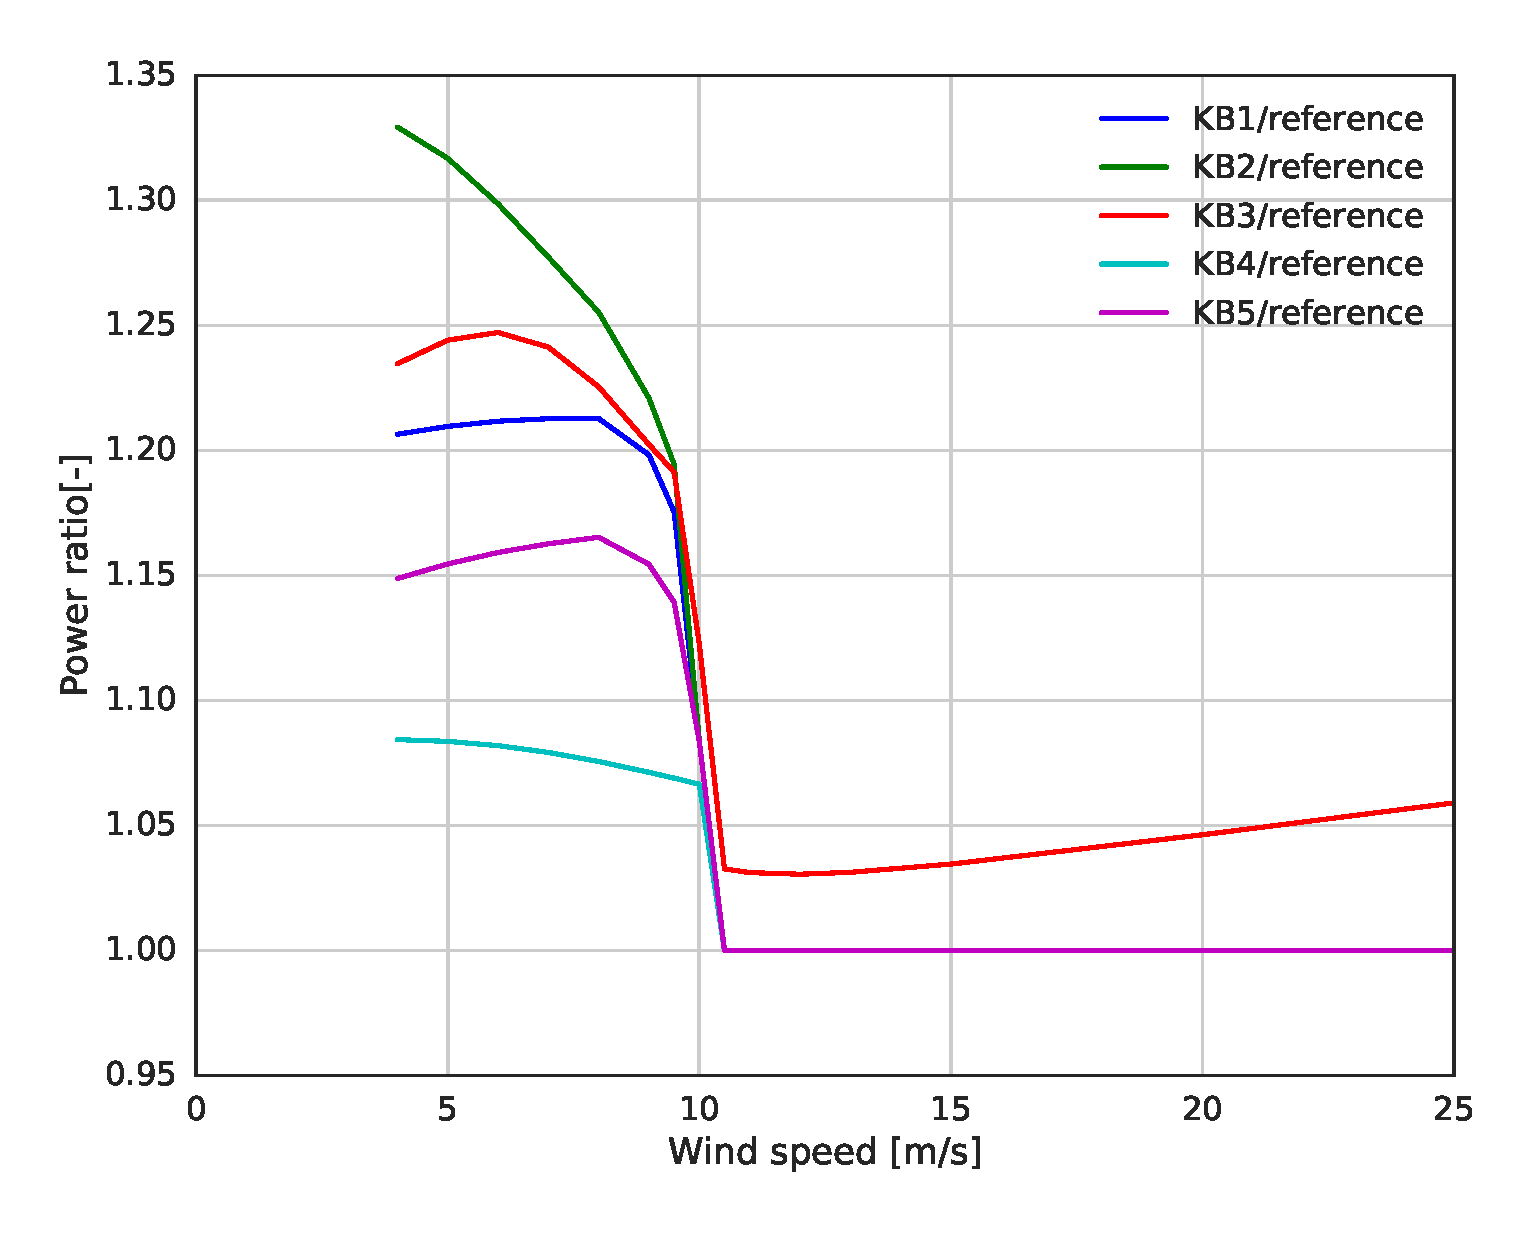
\includegraphics[width=.85\linewidth]{figures/KBcomp_power_ratio.eps}
\end{center}
\caption{Ratio of mechanical power as function of wind speed for the optimized blades relative to the reference.}
\label{fig:powerratio}
\end{figure}

\begin{figure}[pht]
\begin{center}
	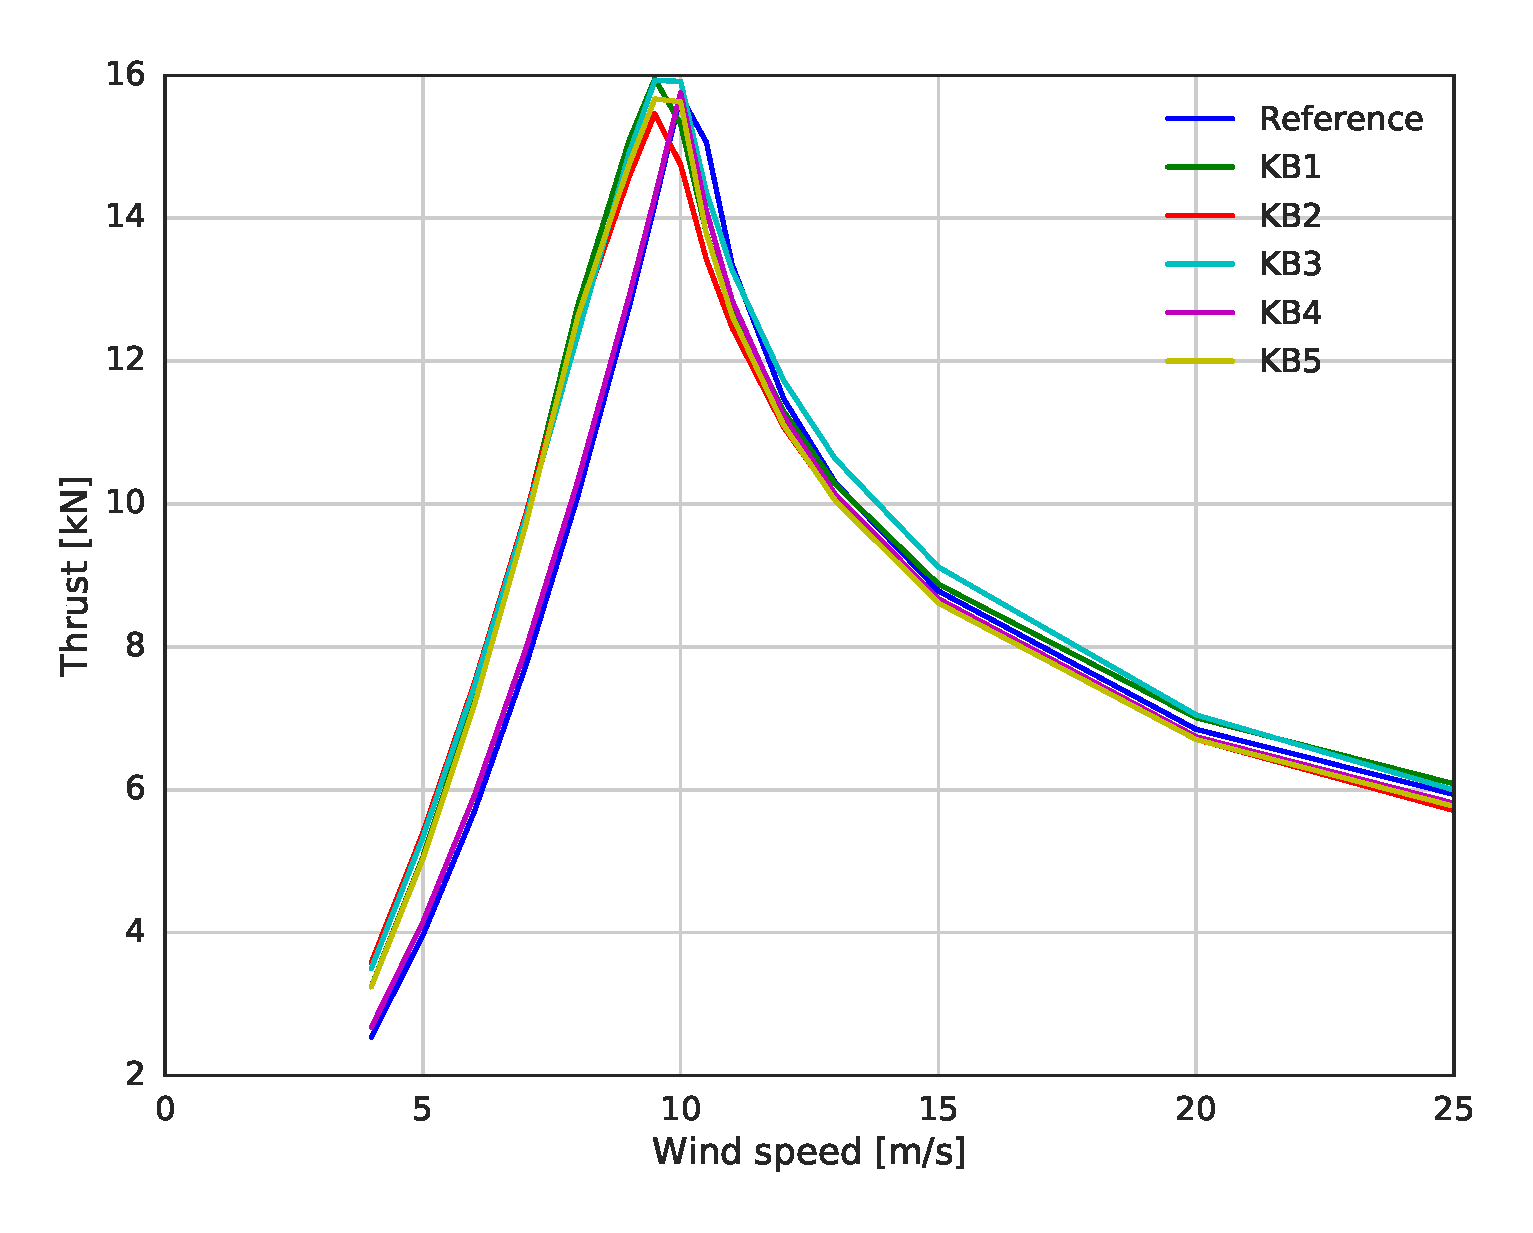
\includegraphics[width=.85\linewidth]{figures/KBcomp_thrust.eps}
\end{center}
\caption{Rotor thrust as function of wind speed for the five optimized blades.}
\label{fig:thrust}
\end{figure}

\begin{figure}[pht]
\begin{center}
	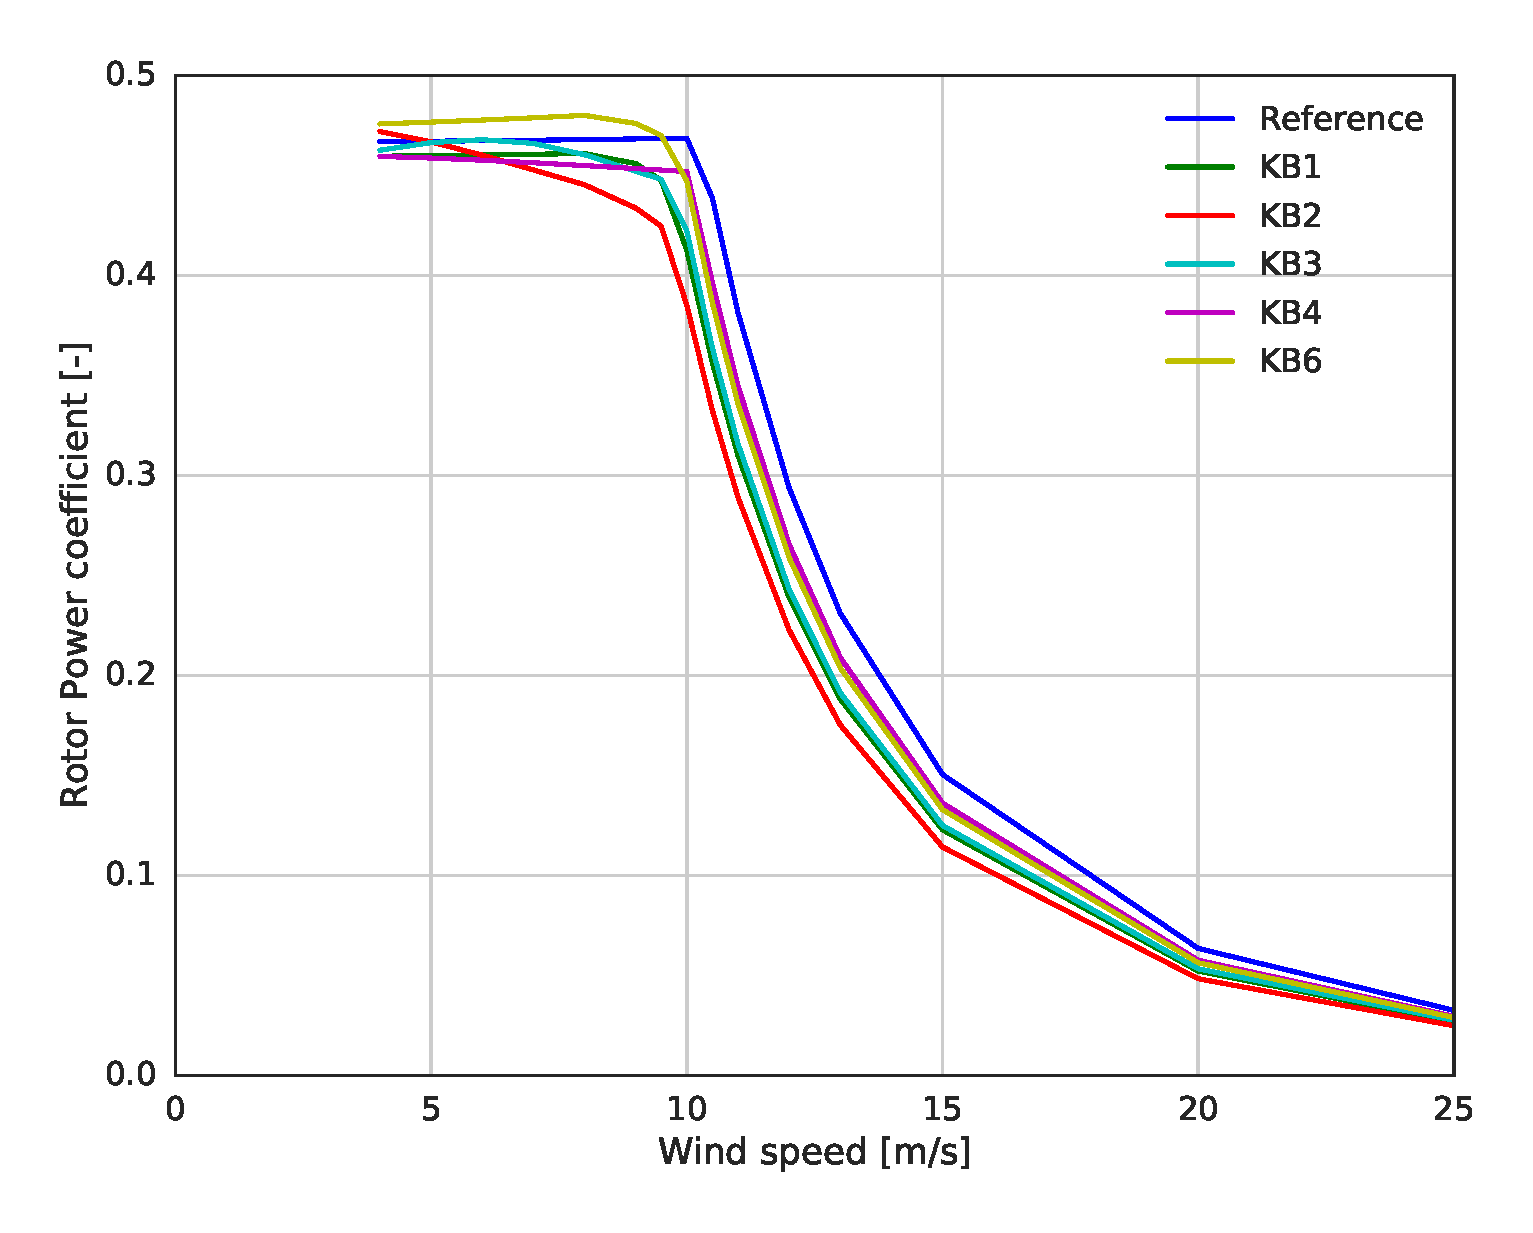
\includegraphics[width=.85\linewidth]{figures/KBcomp_Cp.eps}
\end{center}
\caption{Mechanical power coefficient as function of wind speed for the five optimized blades.}
\label{fig:cp}
\end{figure}

\begin{figure}[pht]
\begin{center}
	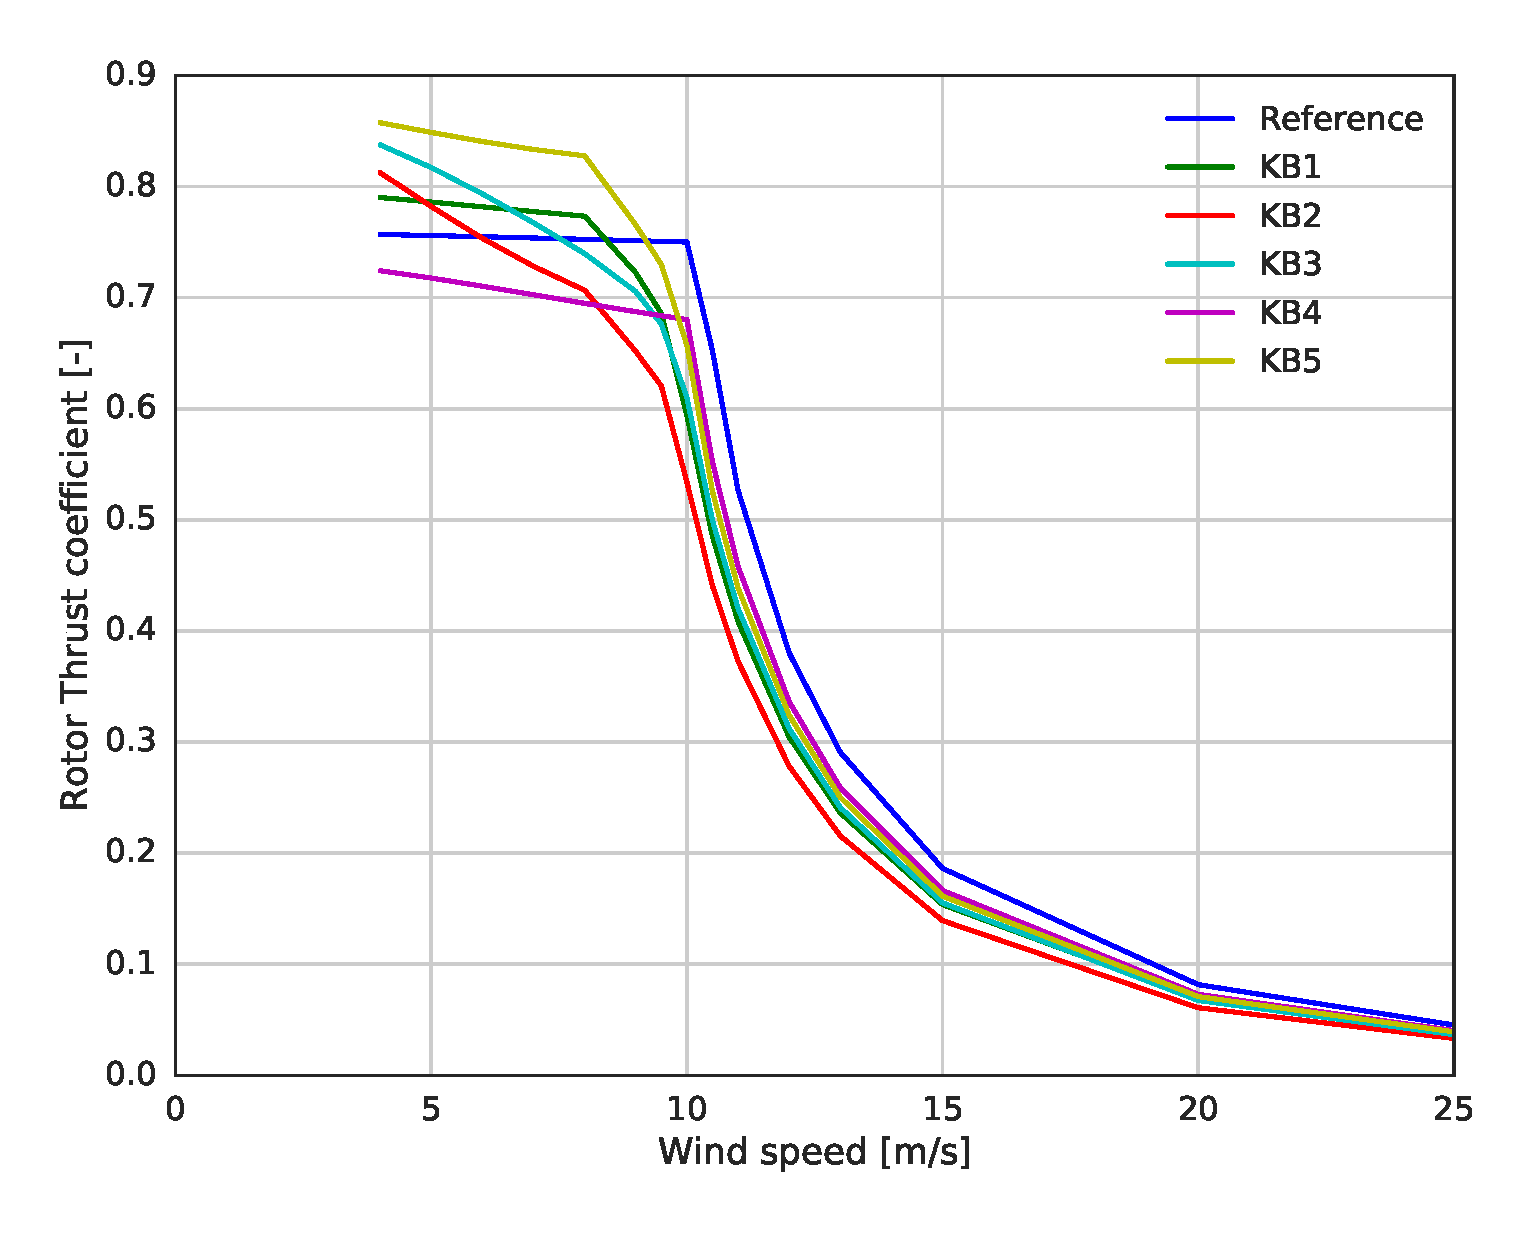
\includegraphics[width=.85\linewidth]{figures/KBcomp_CT.eps}
\end{center}
\caption{Rotor thrust coefficient as function of wind speed for the five optimized blades.}
\label{fig:ct}
\end{figure}

\begin{figure}[pht]
\begin{center}
	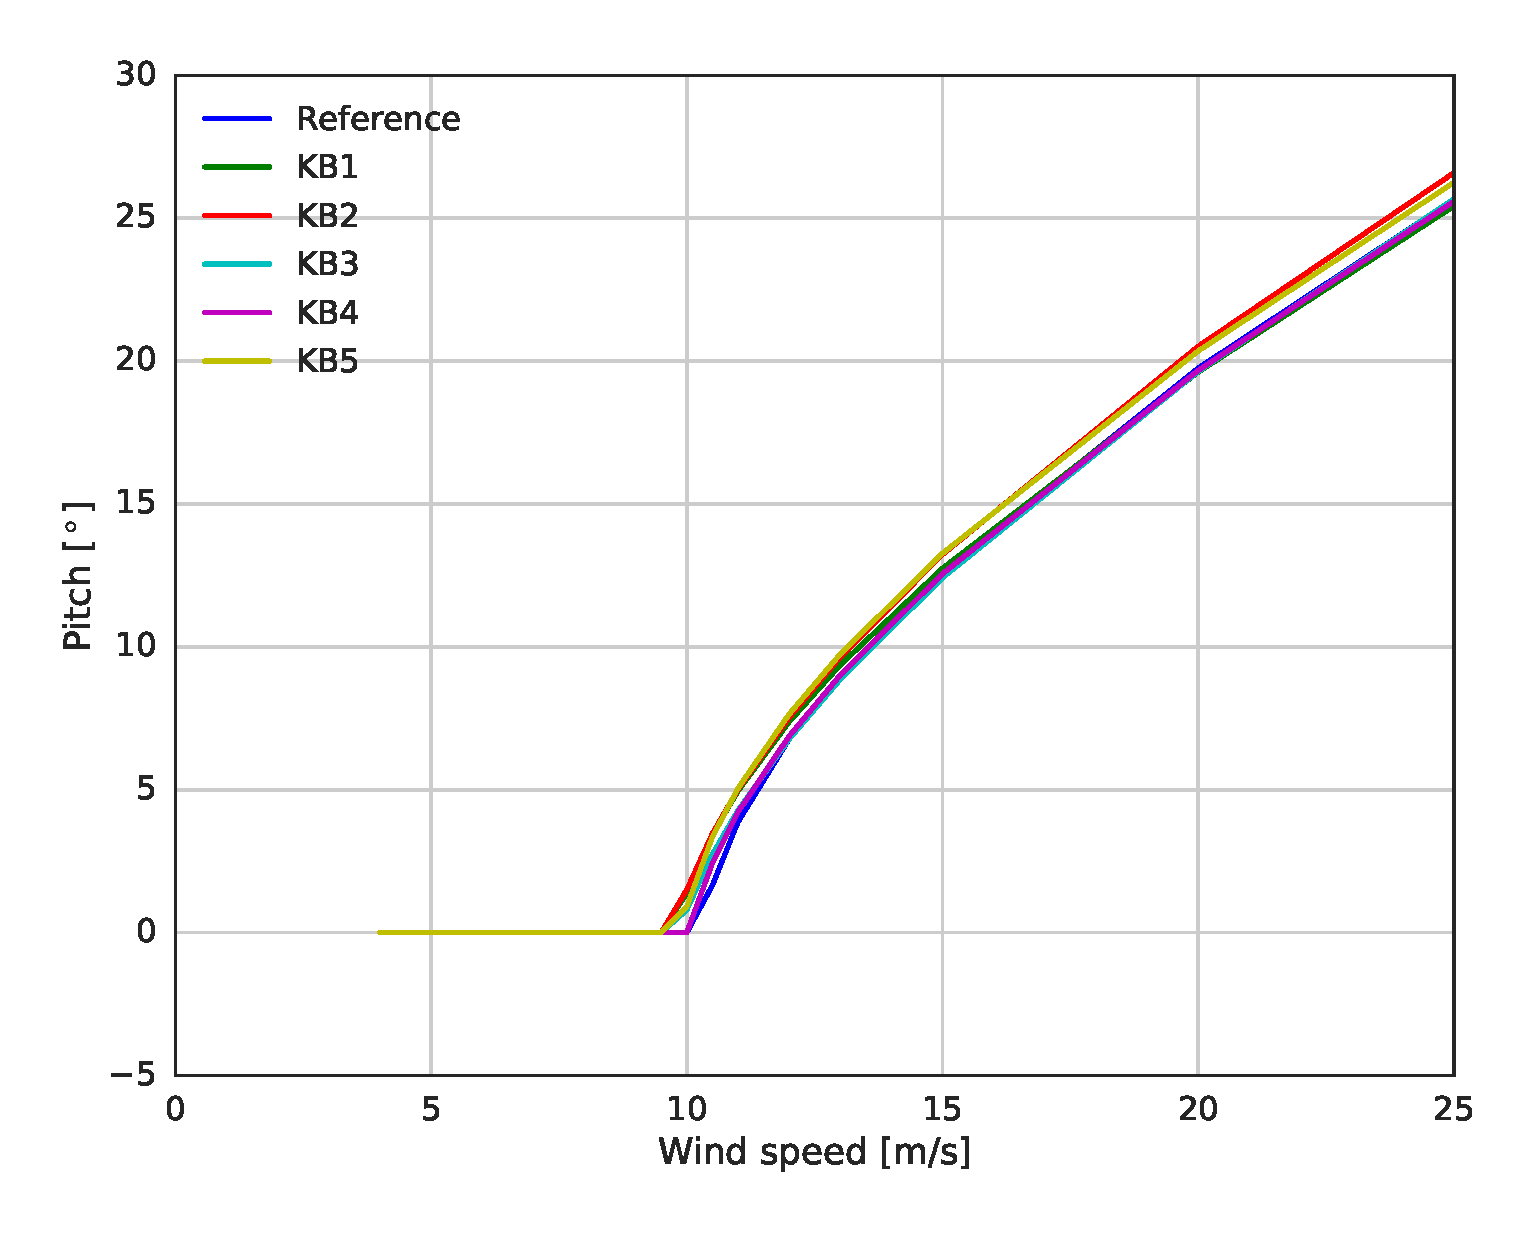
\includegraphics[width=.85\linewidth]{figures/KBcomp_pitch.eps}
\end{center}
\caption{Blade pitch as function of wind speed for the five optimized blades.}
\label{fig:pitch}
\end{figure}

\begin{figure}[pht]
\begin{center}
	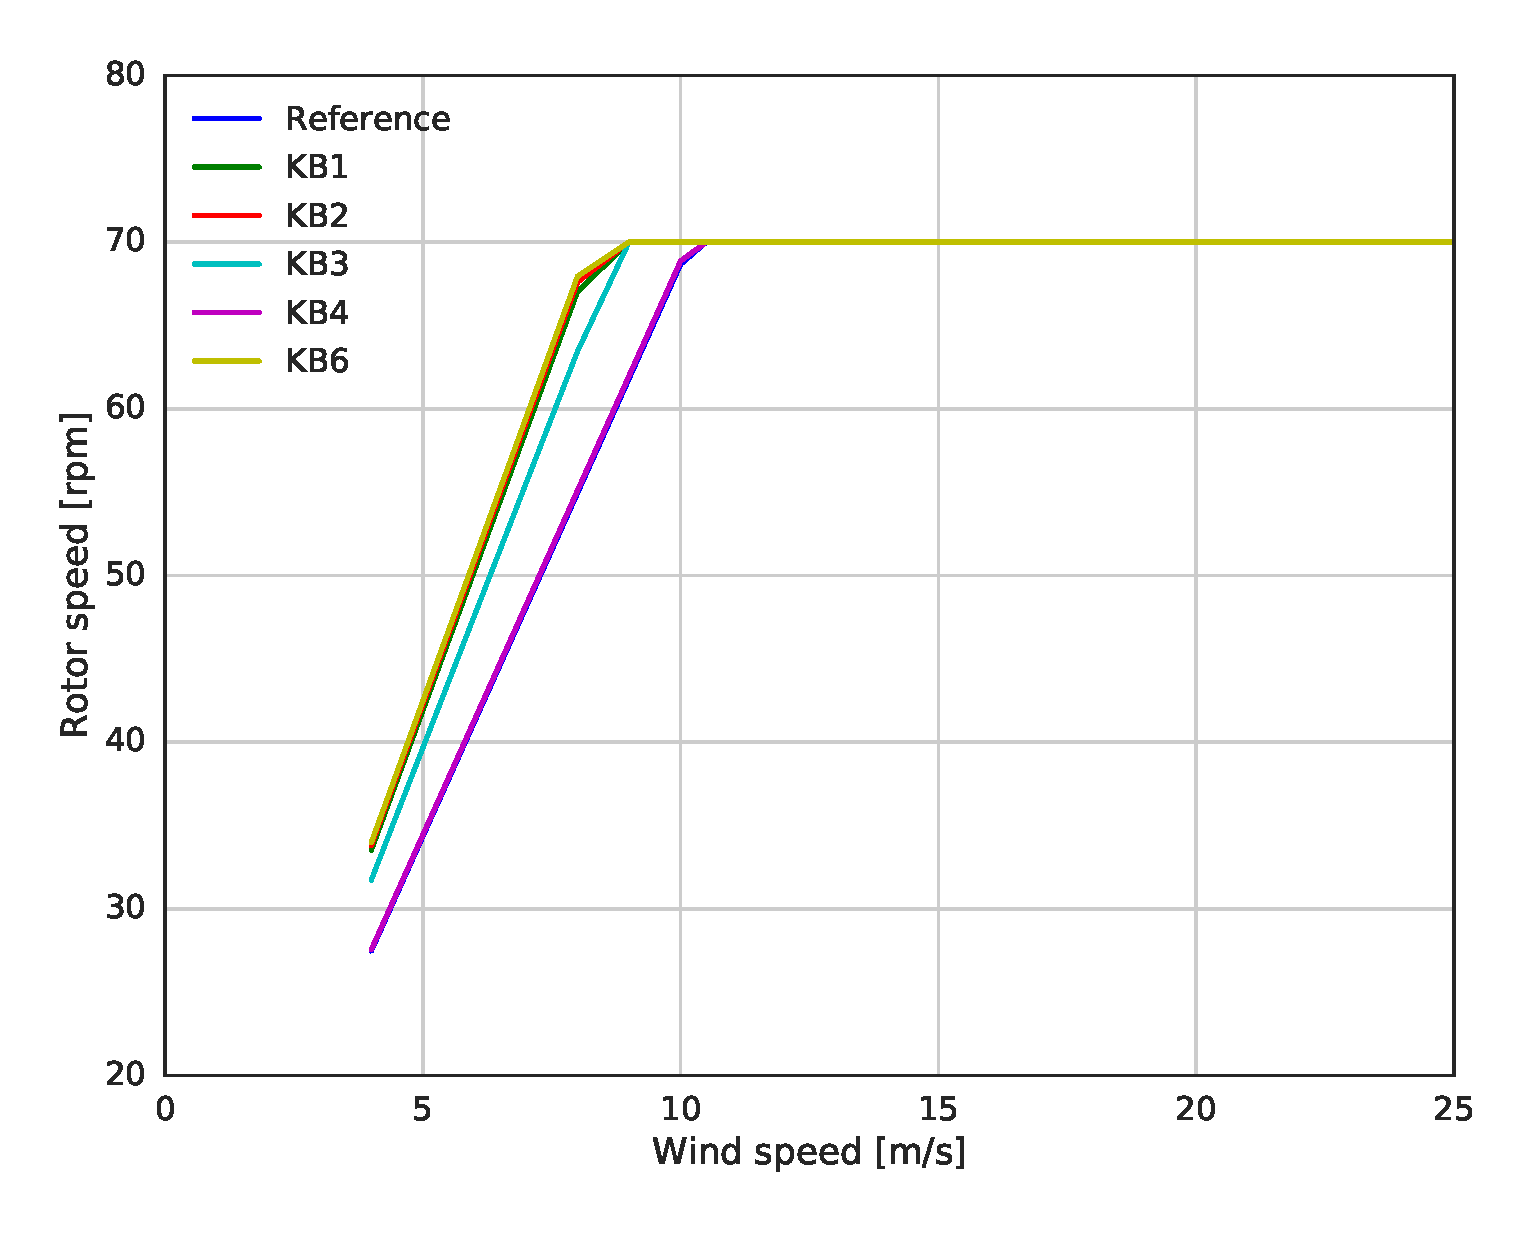
\includegraphics[width=.85\linewidth]{figures/KBcomp_rpm.eps}
\end{center}
\caption{Rotor speed as function of wind speed for the five optimized blades.}
\label{fig:rpm}
\end{figure}

\clearpage

Figures \ref{fig:chord} to \ref{fig:sweep} show the blade planform for the five blades compared to the reference.
All five blades have a more slender planform than the reference resulting from the high TSR, which enables driving down blade mass.
The material coupled blades have higher twist distributions than the non-coupled blades towards the blade tip due to the torsional coupling, as seen in Figure \ref{fig:twist}. 
The optimized blades generally have higher airfoil relative thicknesses, particularly near mid-span, where there are the highest demands for stiffness and strength, as seen in Figure \ref{fig:rthick}. Towards the root the relative thicknesses decrease due to the high chord which provides sufficient blade thickness and therefore stiffness.
The optimizer can also alter the position of the cross-section relative to the blade axis, referred to as pitch axis aft leading edge. This is shown in Figure \ref{fig:p_le}. This affects the positioning of the spar cap within the cross-section as well as the aerodynamic pitch moment.
For all blades, the cross-section is moved forward towards the tip but is somewhat less pronounced for the KB3 and KB4 blades. 

\begin{figure}[pht]
\begin{center}
	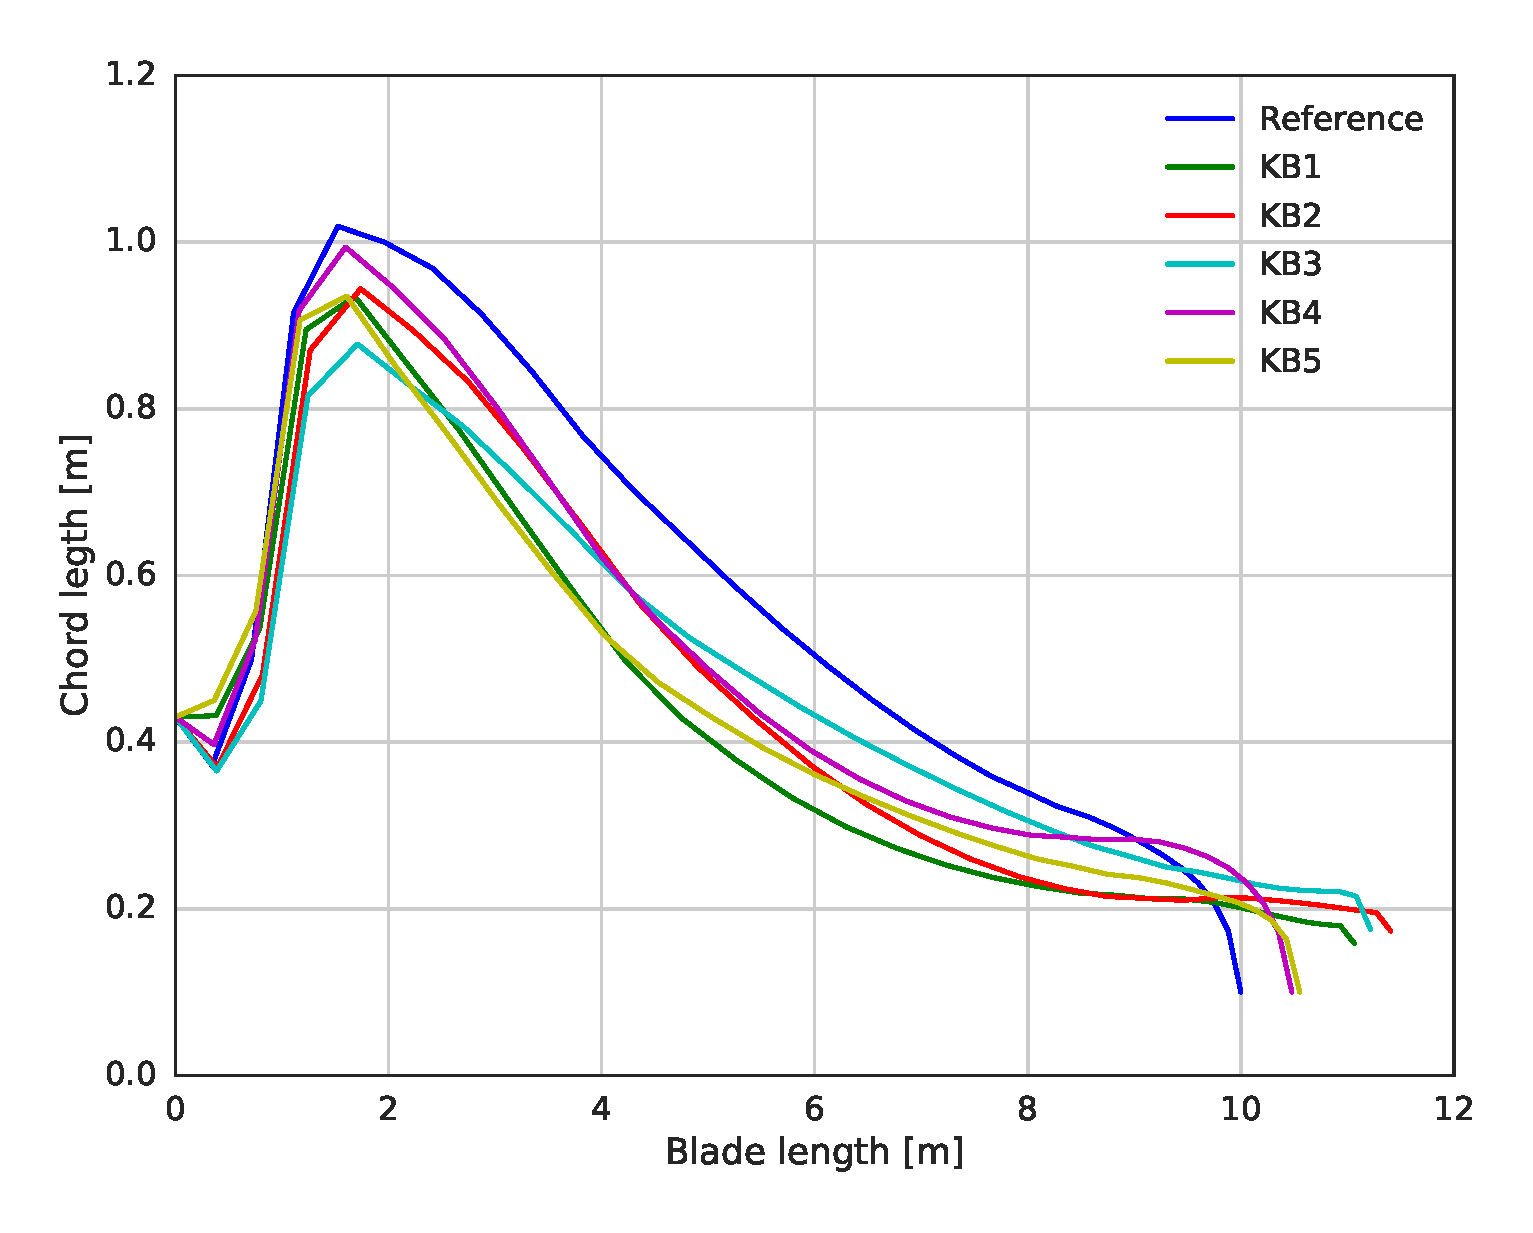
\includegraphics[width=.85\linewidth]{figures/KBcomp_chord.eps}
\end{center}
\caption{Blade chord distributions for the five optimized blades.}
\label{fig:chord}
\end{figure}


\begin{figure}[pht]
\begin{center}
	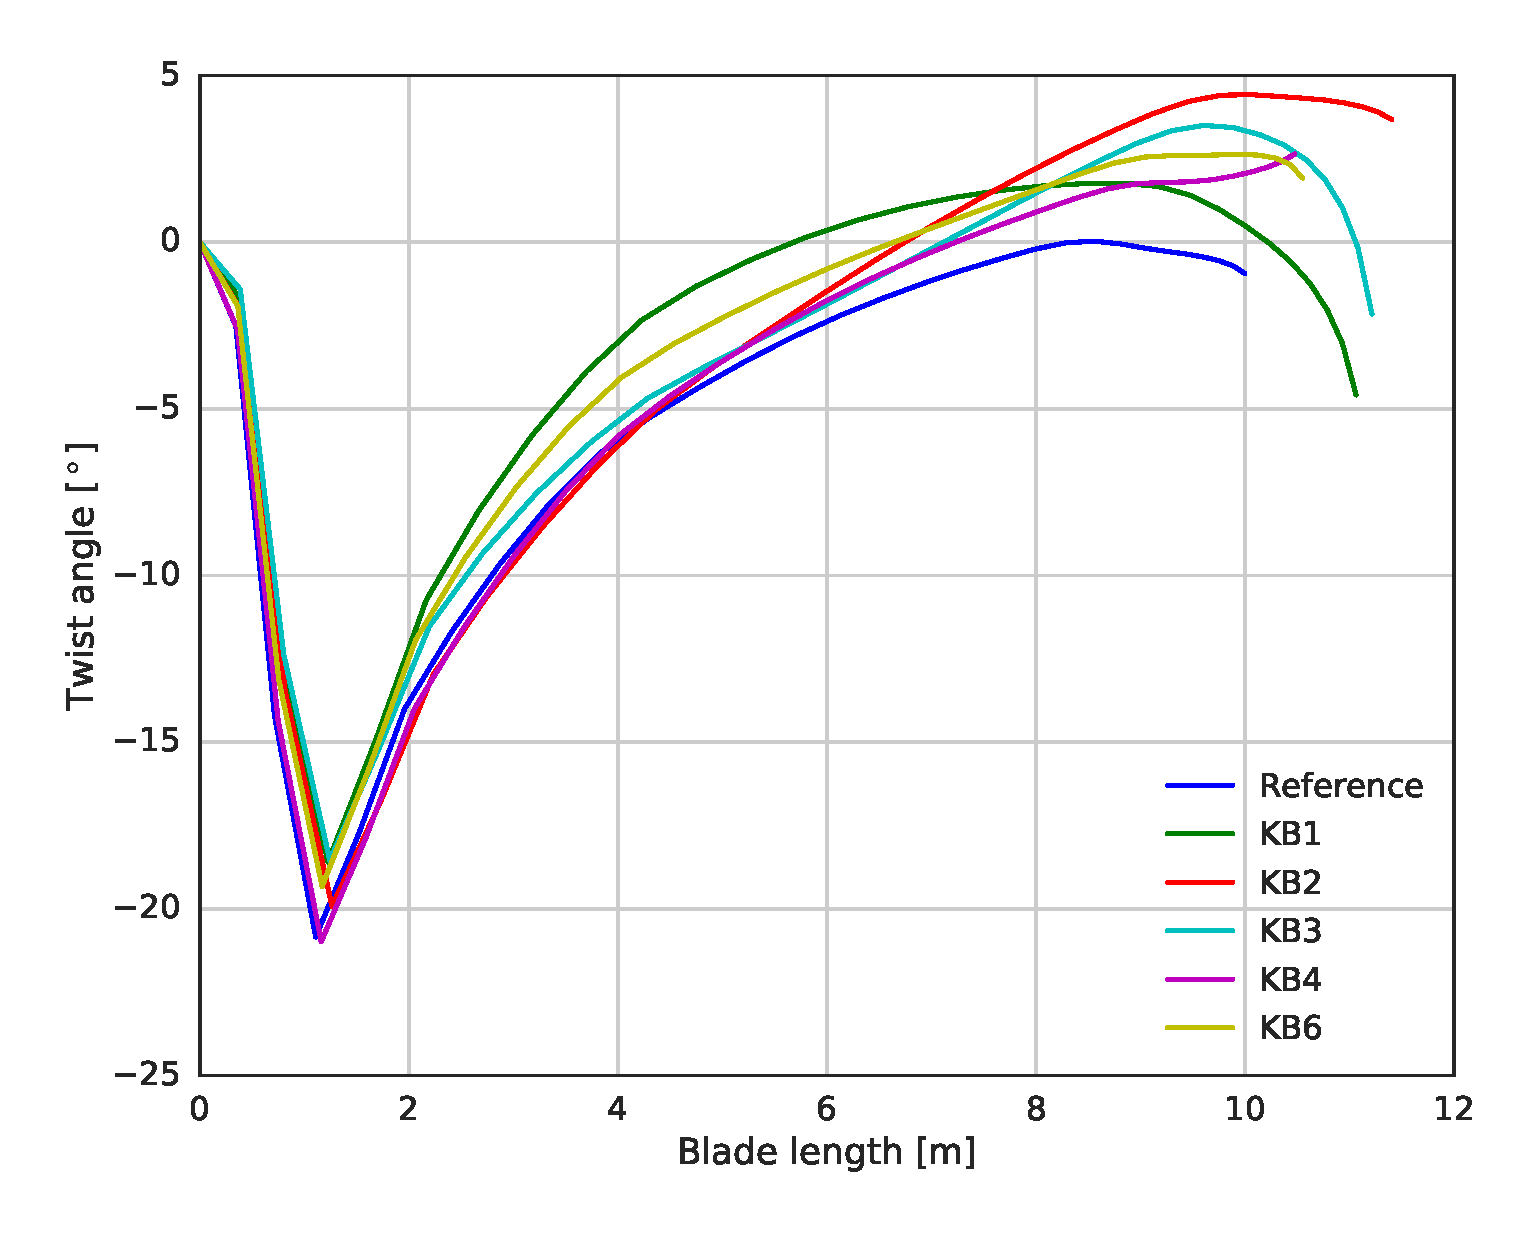
\includegraphics[width=.85\linewidth]{figures/KBcomp_twist.eps}
\end{center}
\caption{Blade twist distributions for the five optimized blades.}
\label{fig:twist}
\end{figure}

\begin{figure}[pht]
\begin{center}
	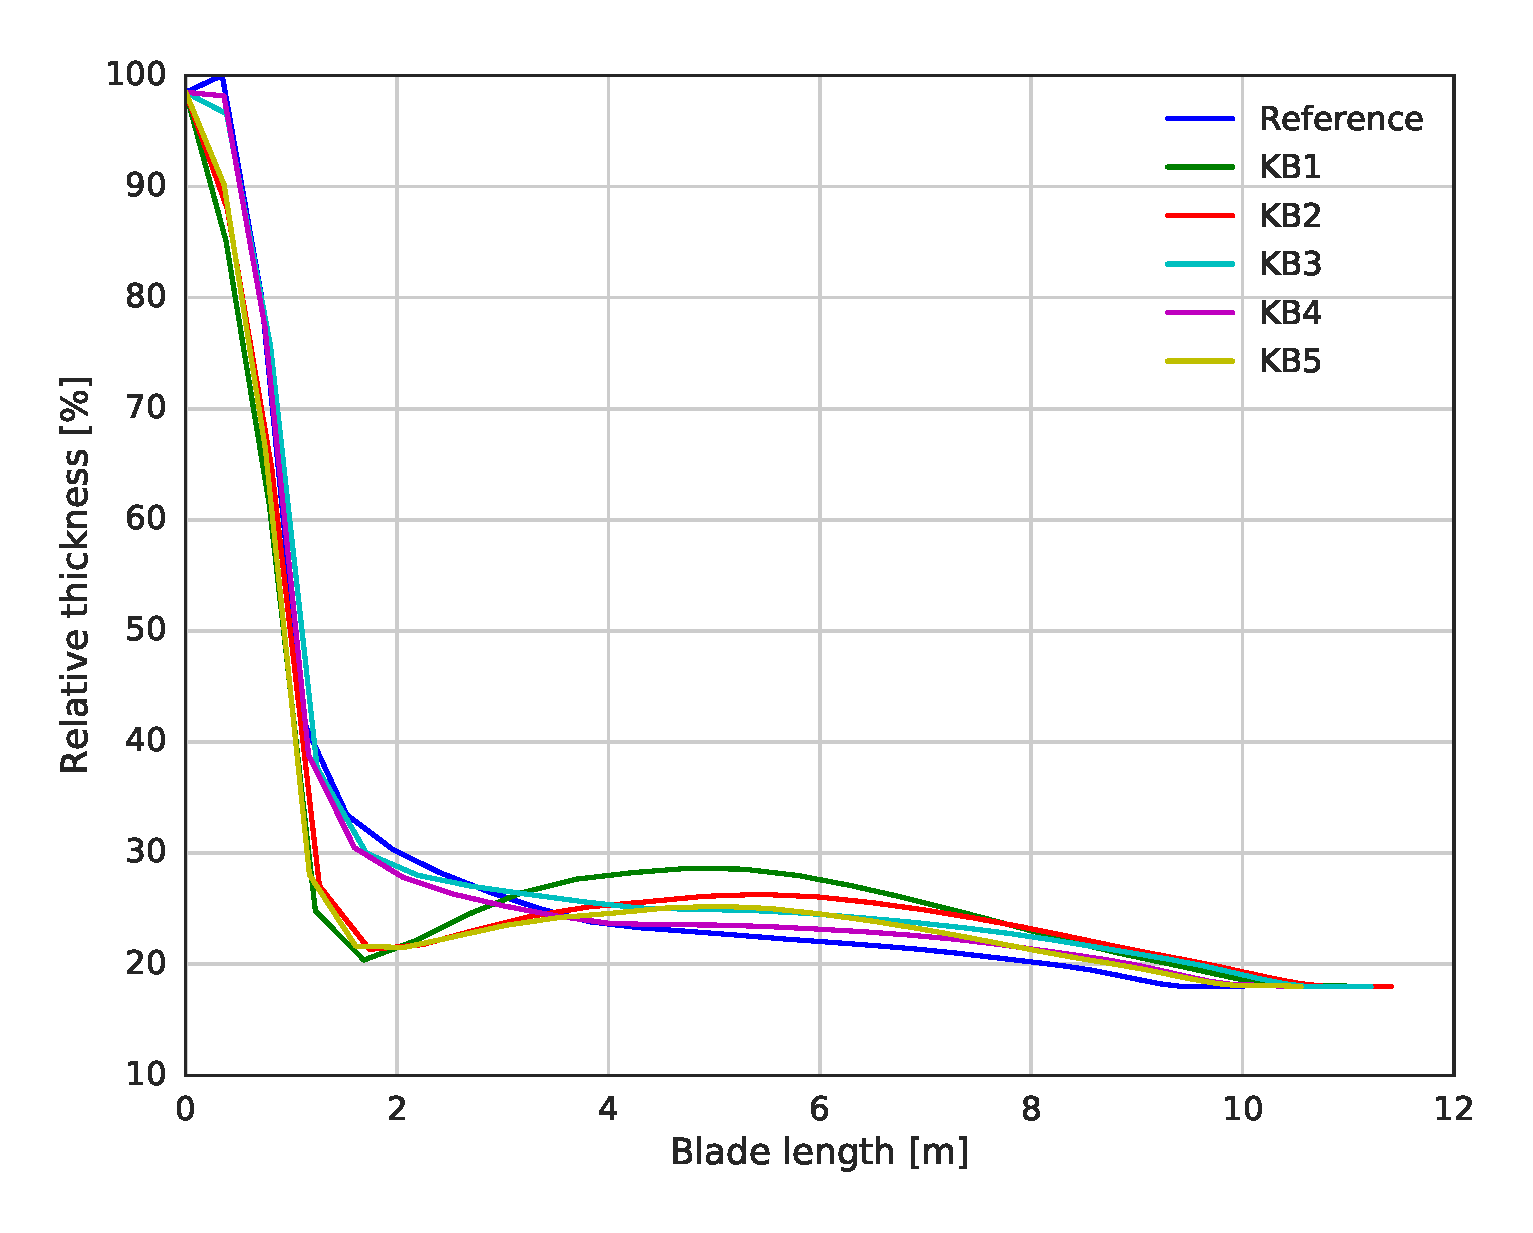
\includegraphics[width=.85\linewidth]{figures/KBcomp_rthick.eps}
\end{center}
\caption{Blade relative thickness distributions for the five optimized blades.}
\label{fig:rthick}
\end{figure}


\begin{figure}[pht]
\begin{center}
	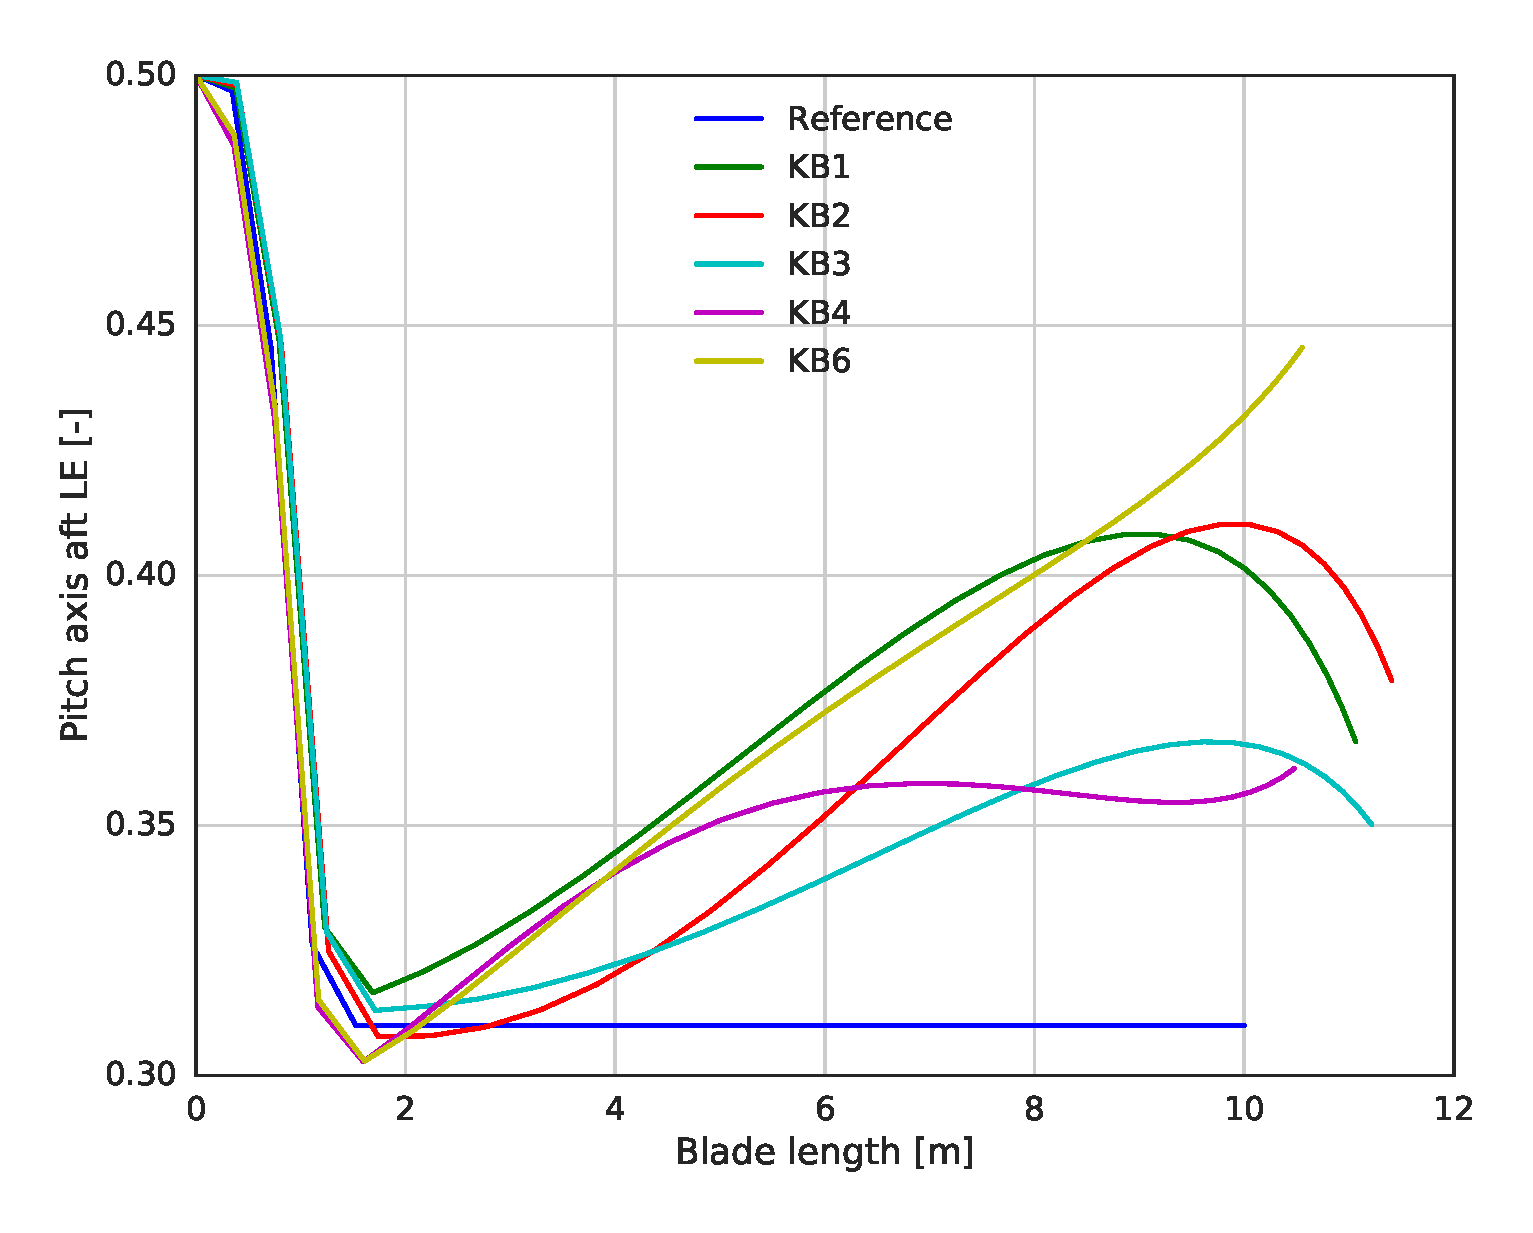
\includegraphics[width=.85\linewidth]{figures/KBcomp_ple.eps}
\end{center}
\caption{Non-dimensionalized blade axis leading edge offset distributions for the five optimized blades.}
\label{fig:p_le}
\end{figure}

\begin{figure}[pht]
\begin{center}
	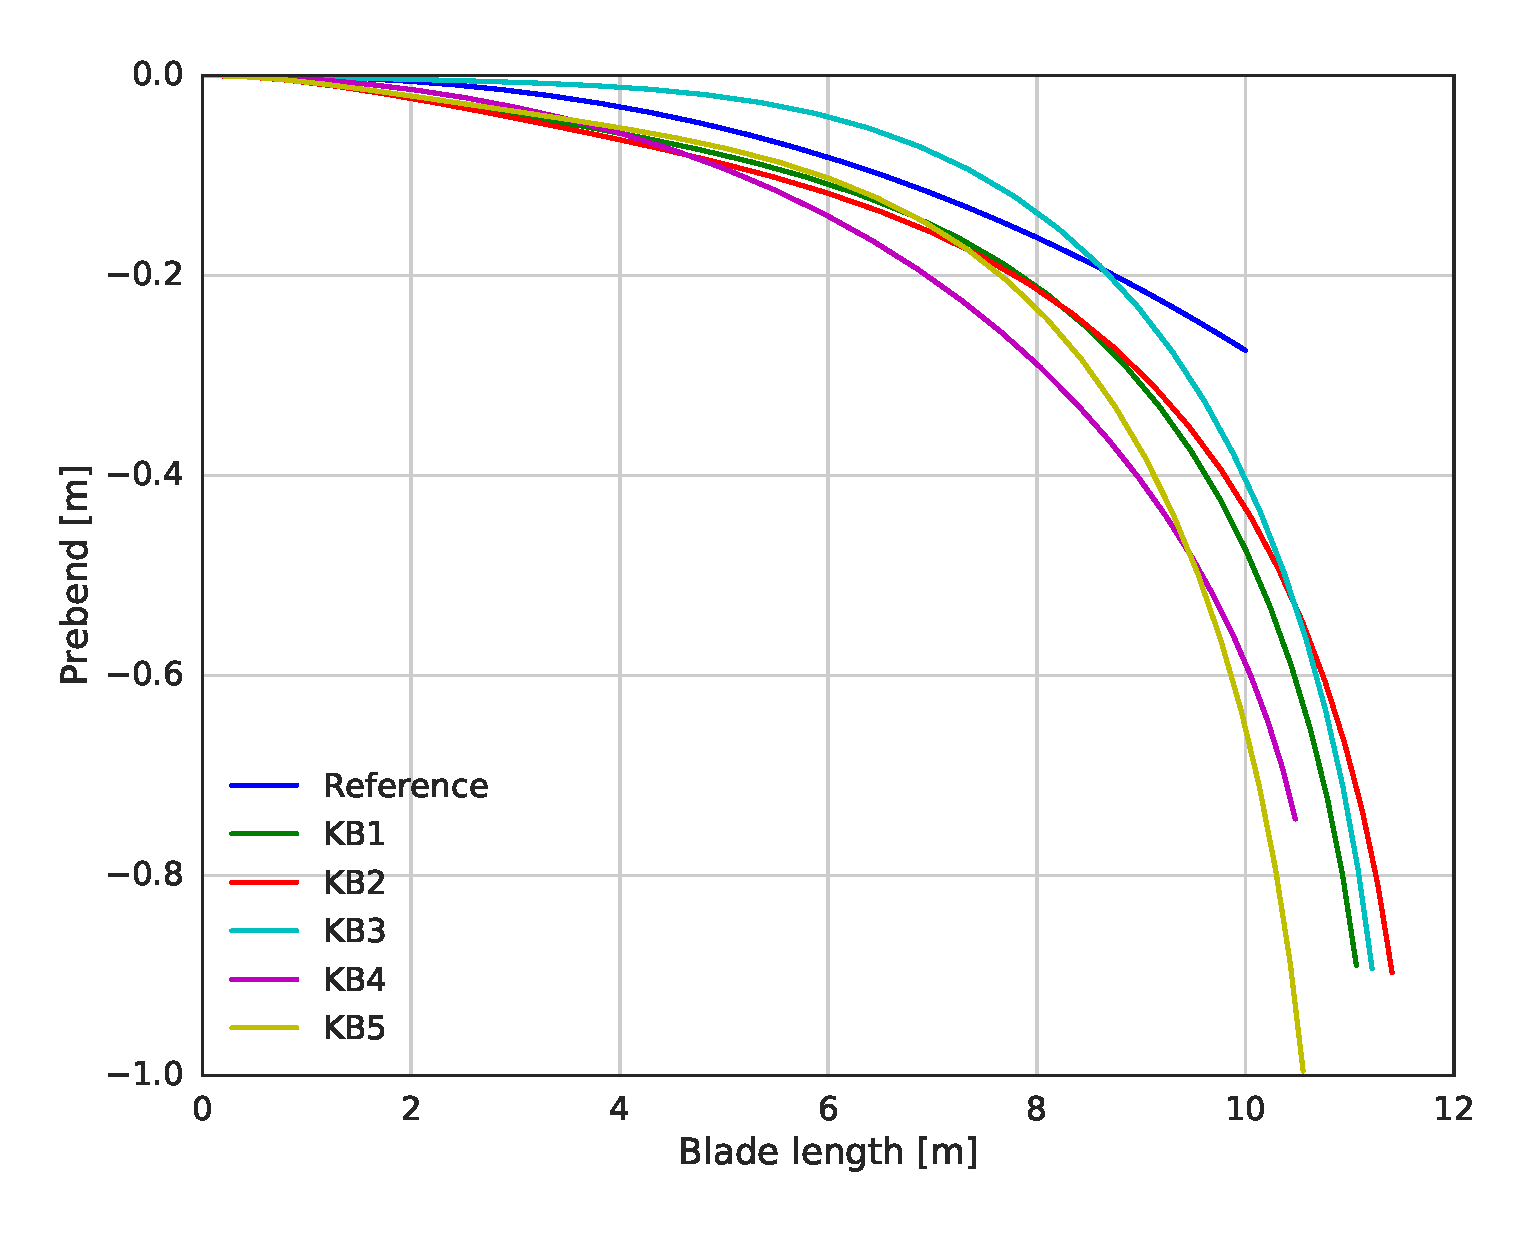
\includegraphics[width=.85\linewidth]{figures/KBcomp_prebend.eps}
\end{center}
\caption{Blade pre-bend distributions for the five optimized blades.}
\label{fig:prebend}
\end{figure}

\begin{figure}[pht]
\begin{center}
	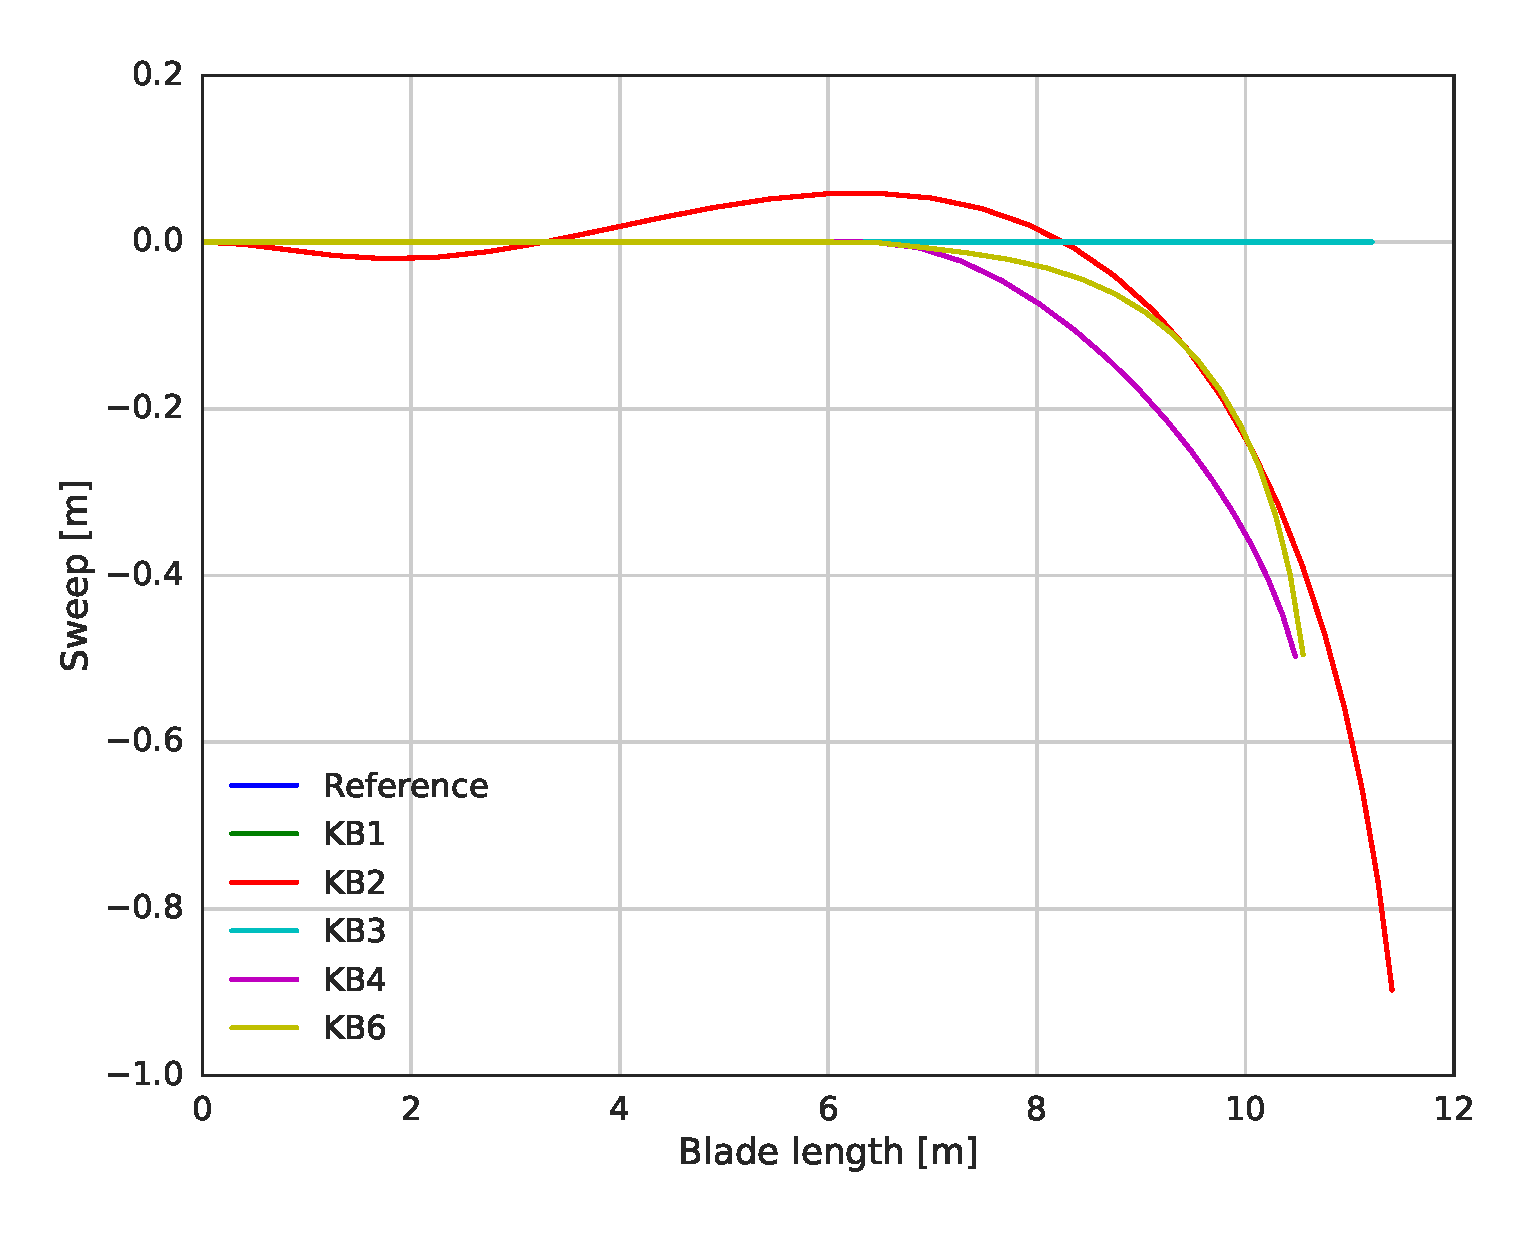
\includegraphics[width=.85\linewidth]{figures/KBcomp_sweep.eps}
\end{center}
\caption{Blade sweep distributions for the five optimized blades.}
\label{fig:sweep}
\end{figure}

\subsection{Structural Design}

The overall structural topology is the same for all five blades, shown in Figure \ref{fig:loftedstructure_baseline_tipview}.
As summarized in the optimization setup, Table \ref{tab:dv_summary}, the spar cap width was allowed to change linearly from root to tip for KB1, KB2 and KB3 optimizations. Figure \ref{fig:capwidth} shows the resulting spar cap widths for the five blade designs compared to the reference design.
The two blades without sweep, KB1 and KB3, result in an increased cap width in the blade root, whereas the swept design of KB2 ends up with a more slender spar cap. Changing cap width did, however, not change the distance between the two main shear webs, see Figure \ref{fig:cross_section_def} for a schematic of the cross-section parametrization.

The spar cap width is not afforded design freedom for the KB4 and KB6 swept blades and hence follow the same trend as the reference case, albeit with higher magnitudes. The increased magnitudes are attributed to the greater lengths seen in the two blades compared to the reference, as it is scaled with length. KB6 has a slightly greater blade length than KB4 as seen in Table \ref{tab:overall_summary}. This is reflected in the spar cap width for KB6 being marginally higher than that of KB4 as seen in Figure \ref{fig:capwidth}. Not affording design freedom in these two blades limits the influence of the spar cap width in affecting the structural stiffnesses in the swept region of the blade. In contrast, the KB2 blade has a decreased spar cap width in the backward swept region contributing to reducing the stiffnesses and thus aiding in bend-twist coupling by facilitating greater torsion towards feather. 

\begin{figure}[pht]
\begin{center}
	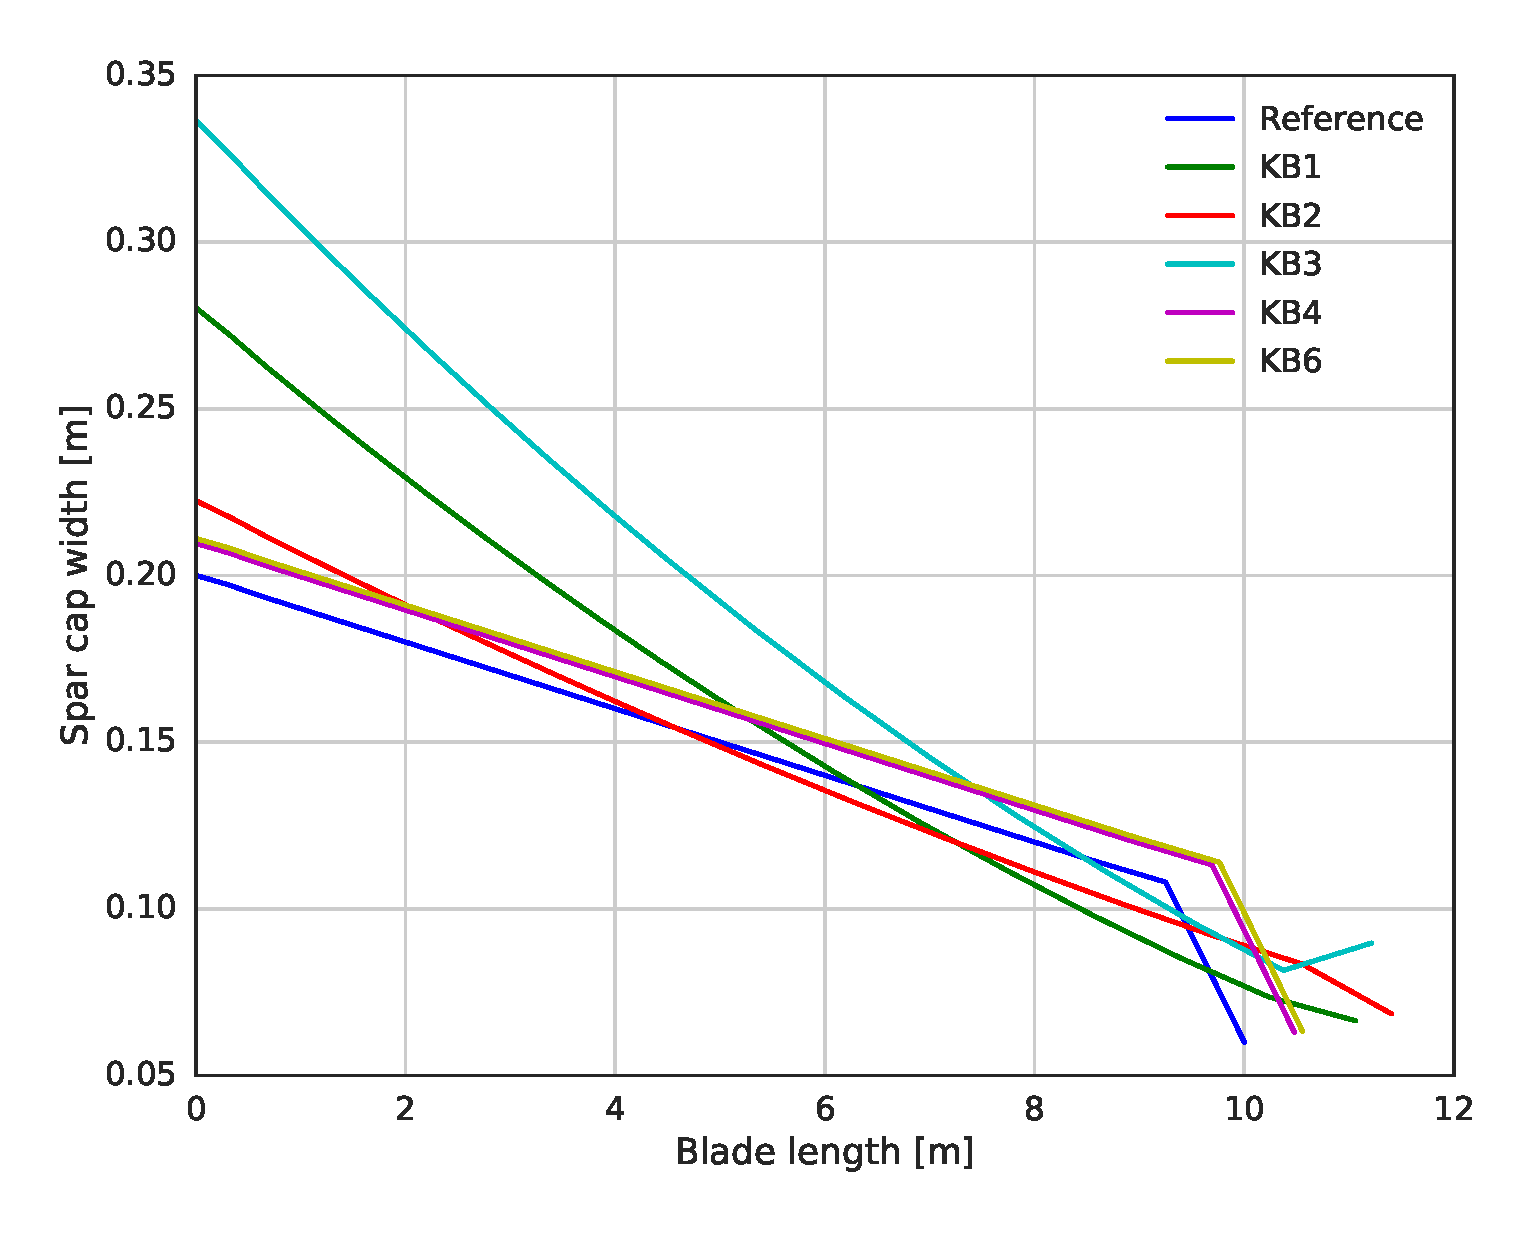
\includegraphics[width=.85\linewidth]{figures/KBcomp_spar_cap_width.eps}
\end{center}
\caption{Blade spar cap width distributions for the five optimized blades.}
\label{fig:capwidth}
\end{figure}

Figures \ref{fig:tipview} and \ref{fig:topview} show the lofted blade shape seen from the tip and top indicating the locations of region division points, spar cap, and shear webs.

\begin{figure}[pht]
\begin{center}
	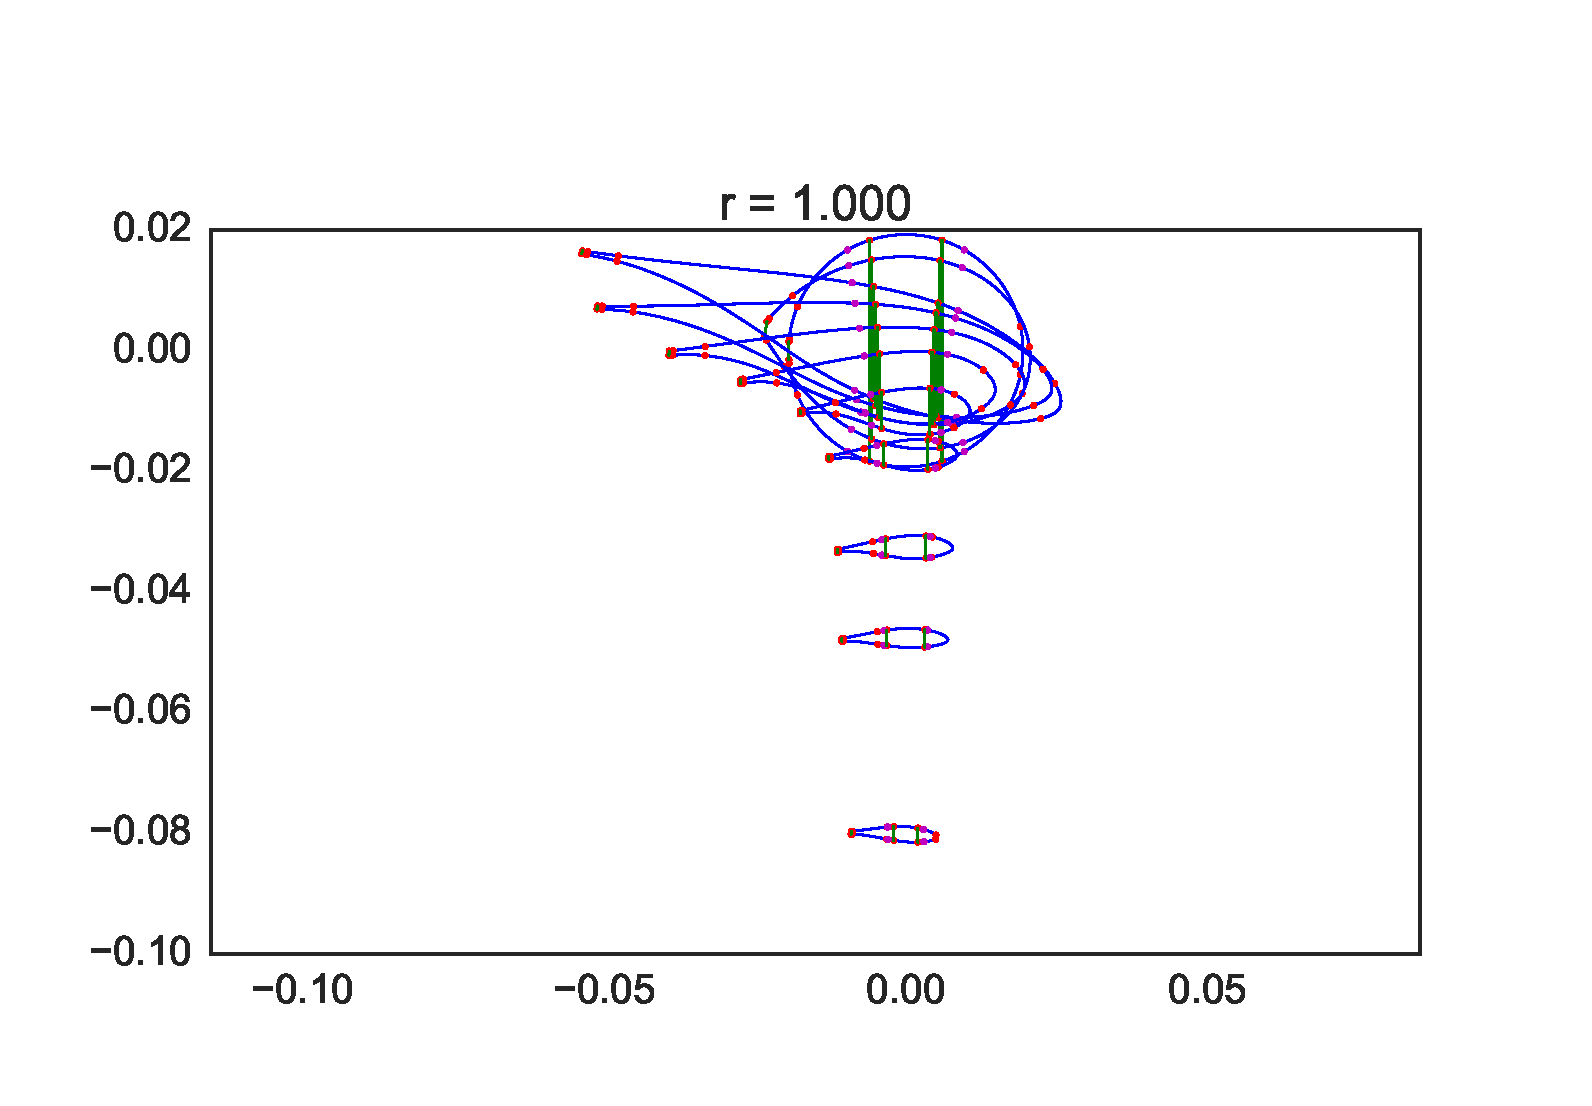
\includegraphics[width=.85\linewidth]{figures/KB1_tipview.eps}
\end{center}
\caption{Tipview schematic of the KB1 blade structure.}
\label{fig:tipview}
\end{figure}

\begin{figure}[pht]
\begin{center}
	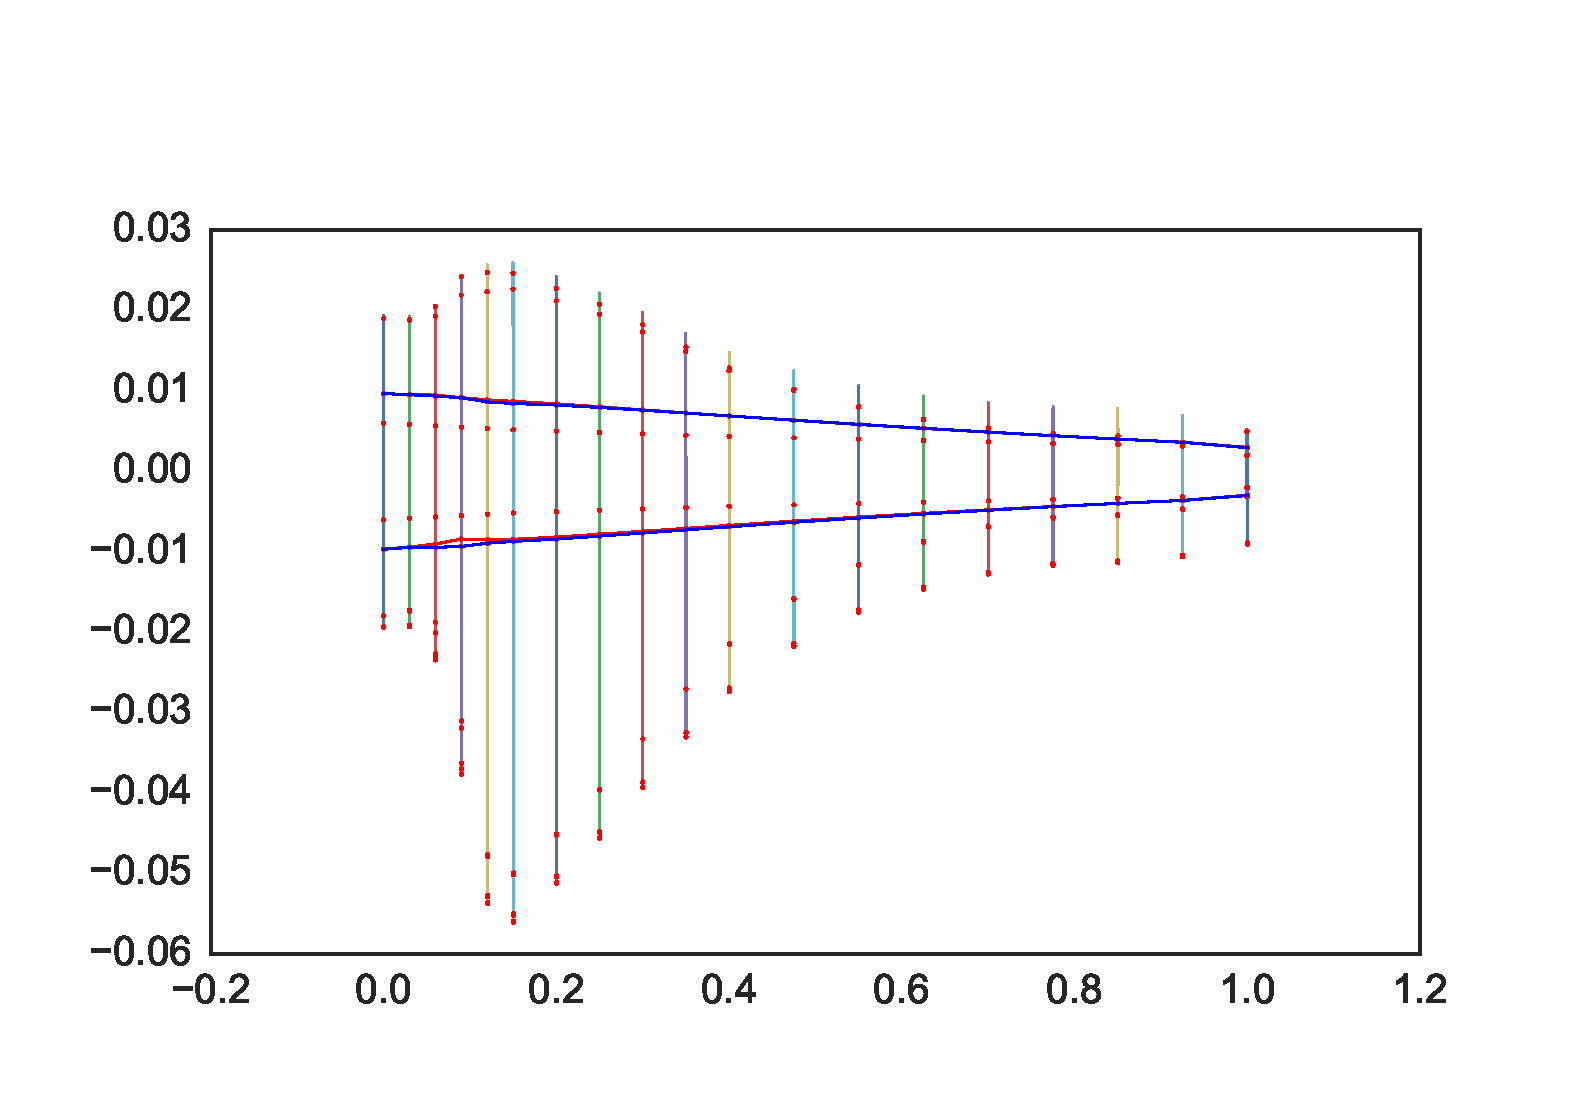
\includegraphics[width=.85\linewidth]{figures/KB1_topview.eps}
\end{center}
\caption{Topview schematic of the KB1 blade structure.}
\label{fig:topview}
\end{figure}

\section{Selected blade design - KB6 swept blade}
\label{sec:final_design}
This section focuses on the evaluation of the selected optimized design that is the KB6 swept blade. Based on the results of the initial optimizations performed in KB1, KB2 and KB3 it was decided to select geometric sweep as the only source of bend-twist coupling. Even though the two coupled designs namely KB2 and KB3, provide similar steady state performance the AEP and power produced by the swept blade design in KB2 is superior to that of the material coupled design in KB3. This can be seen from Figure \ref{fig:KB_AEP} and Figure \ref{fig:powerratio}. Hence, a swept design was selected for the final blade. Furthermore, in order to facilitate ease of manufacturing of the blades only backward sweep is allowed in the design with a maximum value limited to almost half the value of that chosen for the KB2 swept blade design. Additionally, an extra layer of triax material is added throughout the blade that is not allowed any design freedom. These restrictions limit the extent to which the optimization could leverage the load reductions caused by the geometric coupling to increase the blade length and hence produce greater AEP than possible with the current constraints in place. Thus, as a result of the additional constraints the optimized KB6 design produces less power than the KB2 design.

\subsection{Multidisciplinary optimization}
\label{subsec:MDO}
The value of the objective function for every iteration of the optimizer is shown in Figure \ref{fig:KB6_objf}. The objective function has been defined in Equation \ref{eqn:objective} and it starts with a value of $-1$ which represents the reference blade. As the optimizer evaluates the design space and leverages the design variables, objective and constrains the changes in the design with each iteration alters the value of the objective function. The aim is to minimize the objective function that is to obtain the highest attainable magnitude of the objective function which corresponds to the maximization of the AEP. It is seen in Figure \ref{fig:KB6_objf} that the objective function represented in blue, decreases with increasing optimizer iterations indicating a successful progression of the problem. As the optimizer solves for the optimal design it inadvertently attains designs from the possible design space which exhibit violations of the constraints imposed on the problem. The constraint violations are shown in red on a log scale. The green dots on the objective function curve represent the attained designs which adhere to the bounds set by the various constraints. The chosen design is the minimum value of the objective function for which no constraint violation has been recorded.

The constraints imposed on the problem have been introduced in Table \ref{tab:con_summary}. Figure \ref{fig:KB6_cons} represents the absolute values of the constraints normalised by their corresponding maximum limits. These constraints have been recorded at the chosen optimal solution of the design. The constraint that has a value which is more than 90\% of its maximum limit is considered to be active and is responsible for affecting the obtained solution. The active constraints from Figure \ref{fig:KB6_cons} are shown in Table \ref{tab:KB6_cons}.

\begin{table}[!ht]
\centering
\caption{Active constraints for KB6}
\label{tab:KB6_cons}
\begin{tabular}{|l|l|}
\hline
 Quantity [-]             & Description           \\
\hline
Q\_con                    &  Steady state thrust  \\
Mx\_con                   &  Steady state flapwise root bending moment    \\
tip\_pos\_b2              &  Blade tip deflection from reduced DLB for blade 2 \\
pb\_con                   &  Prebend    \\
sw\_con                   &  Sweep                  \\
tip\_pos\_b3              &  Blade tip deflection from reduced DLB for blade 3             \\
blade\_failure\_index\_ks &  Blade failure index or strain index  \\
MzBR3\_max                &  Maximum blade root torsion for blade 3 from reduced DLB \\
FyTT\_min                 &  Tower top flapwise force from reduced DLB\\
MzBR1\_max                &  Maximum blade root torsion for blade 1 from reduced DLB \\
tip\_pos\_b1              &  Blade tip deflection from reduced DLB for blade 1 \\
T\_con                    &  Steady state rotor thrust force \\
MxTB\_con                 &  Tower bottom fore-aft bending moment from reduced DLB\\
mass\_con                  &  Blade mass      \\
\hline
\end{tabular}
\end{table}

%% optimization and cons opt
\begin{figure}[pht]
\begin{center}
	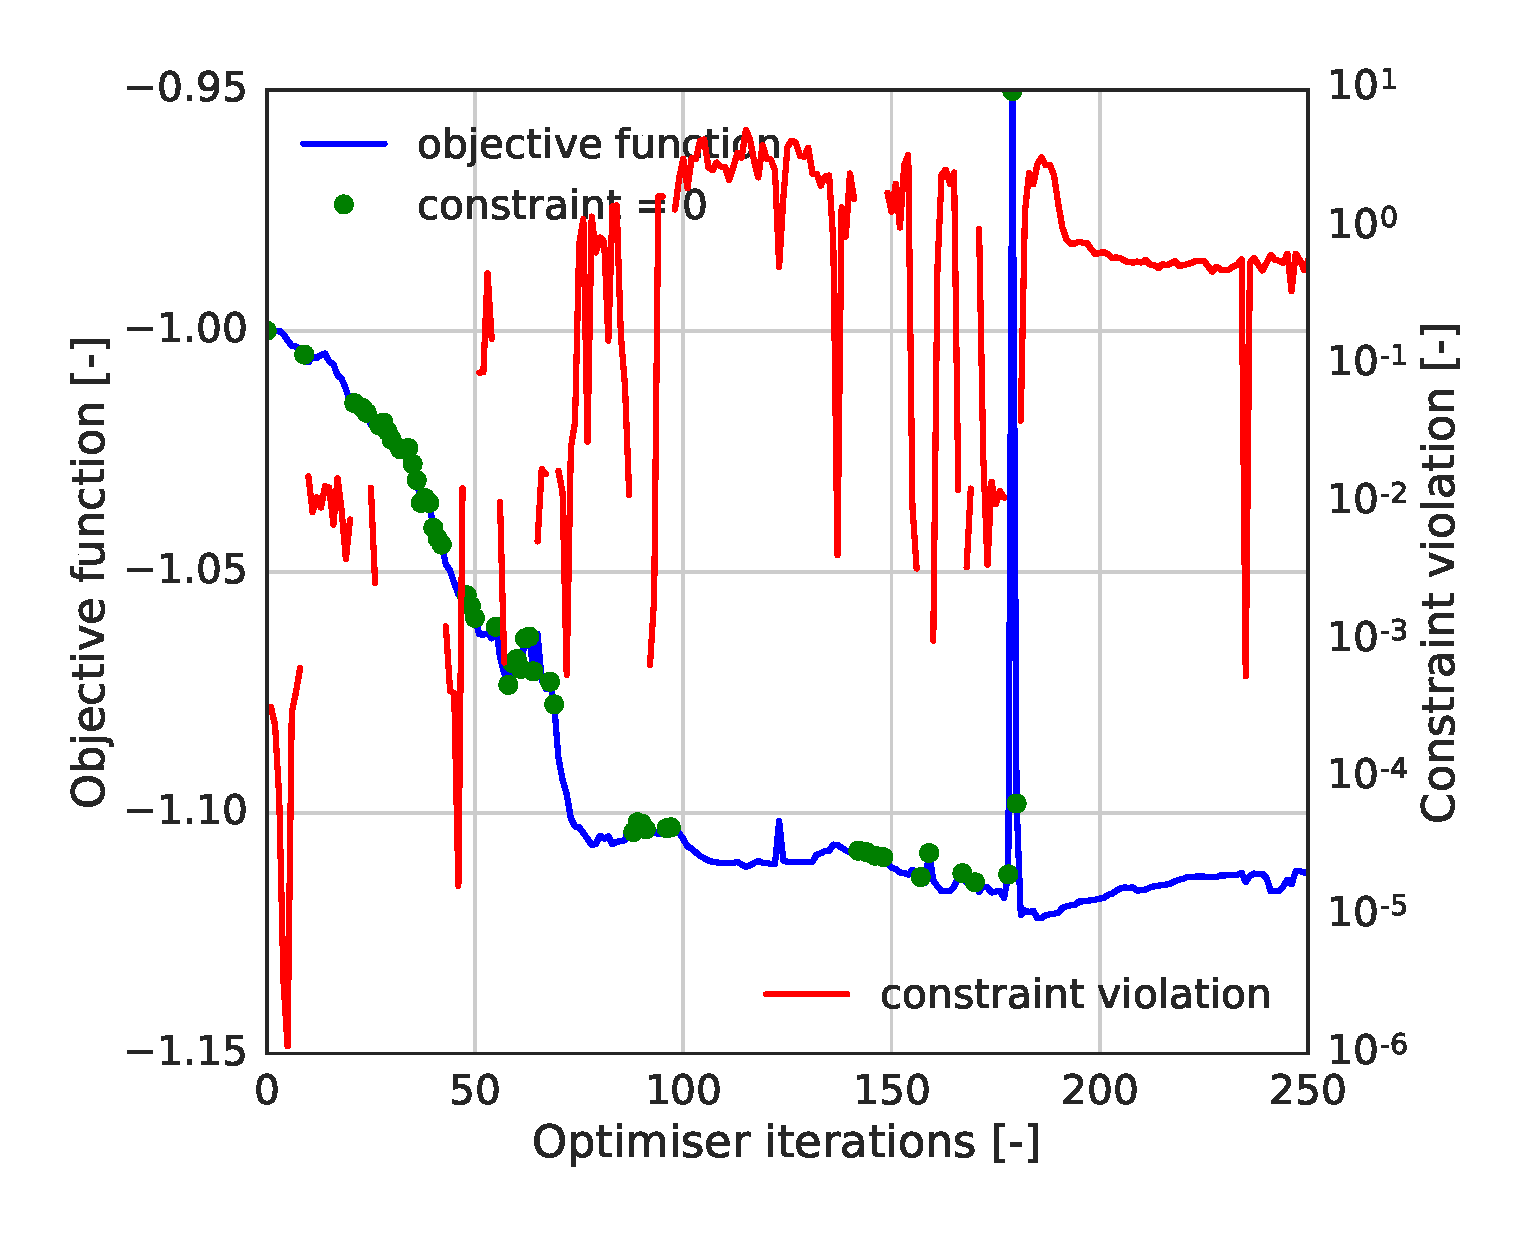
\includegraphics[width=.85\linewidth]{figures/KB6_final/KB6_obj_cons_ipopt.eps}
\end{center}
\caption{Evolution of objective function and constraint violation for increasing iterations of the optimizer.}
\label{fig:KB6_objf}
\end{figure}

\begin{figure}[pht]
\begin{center}
	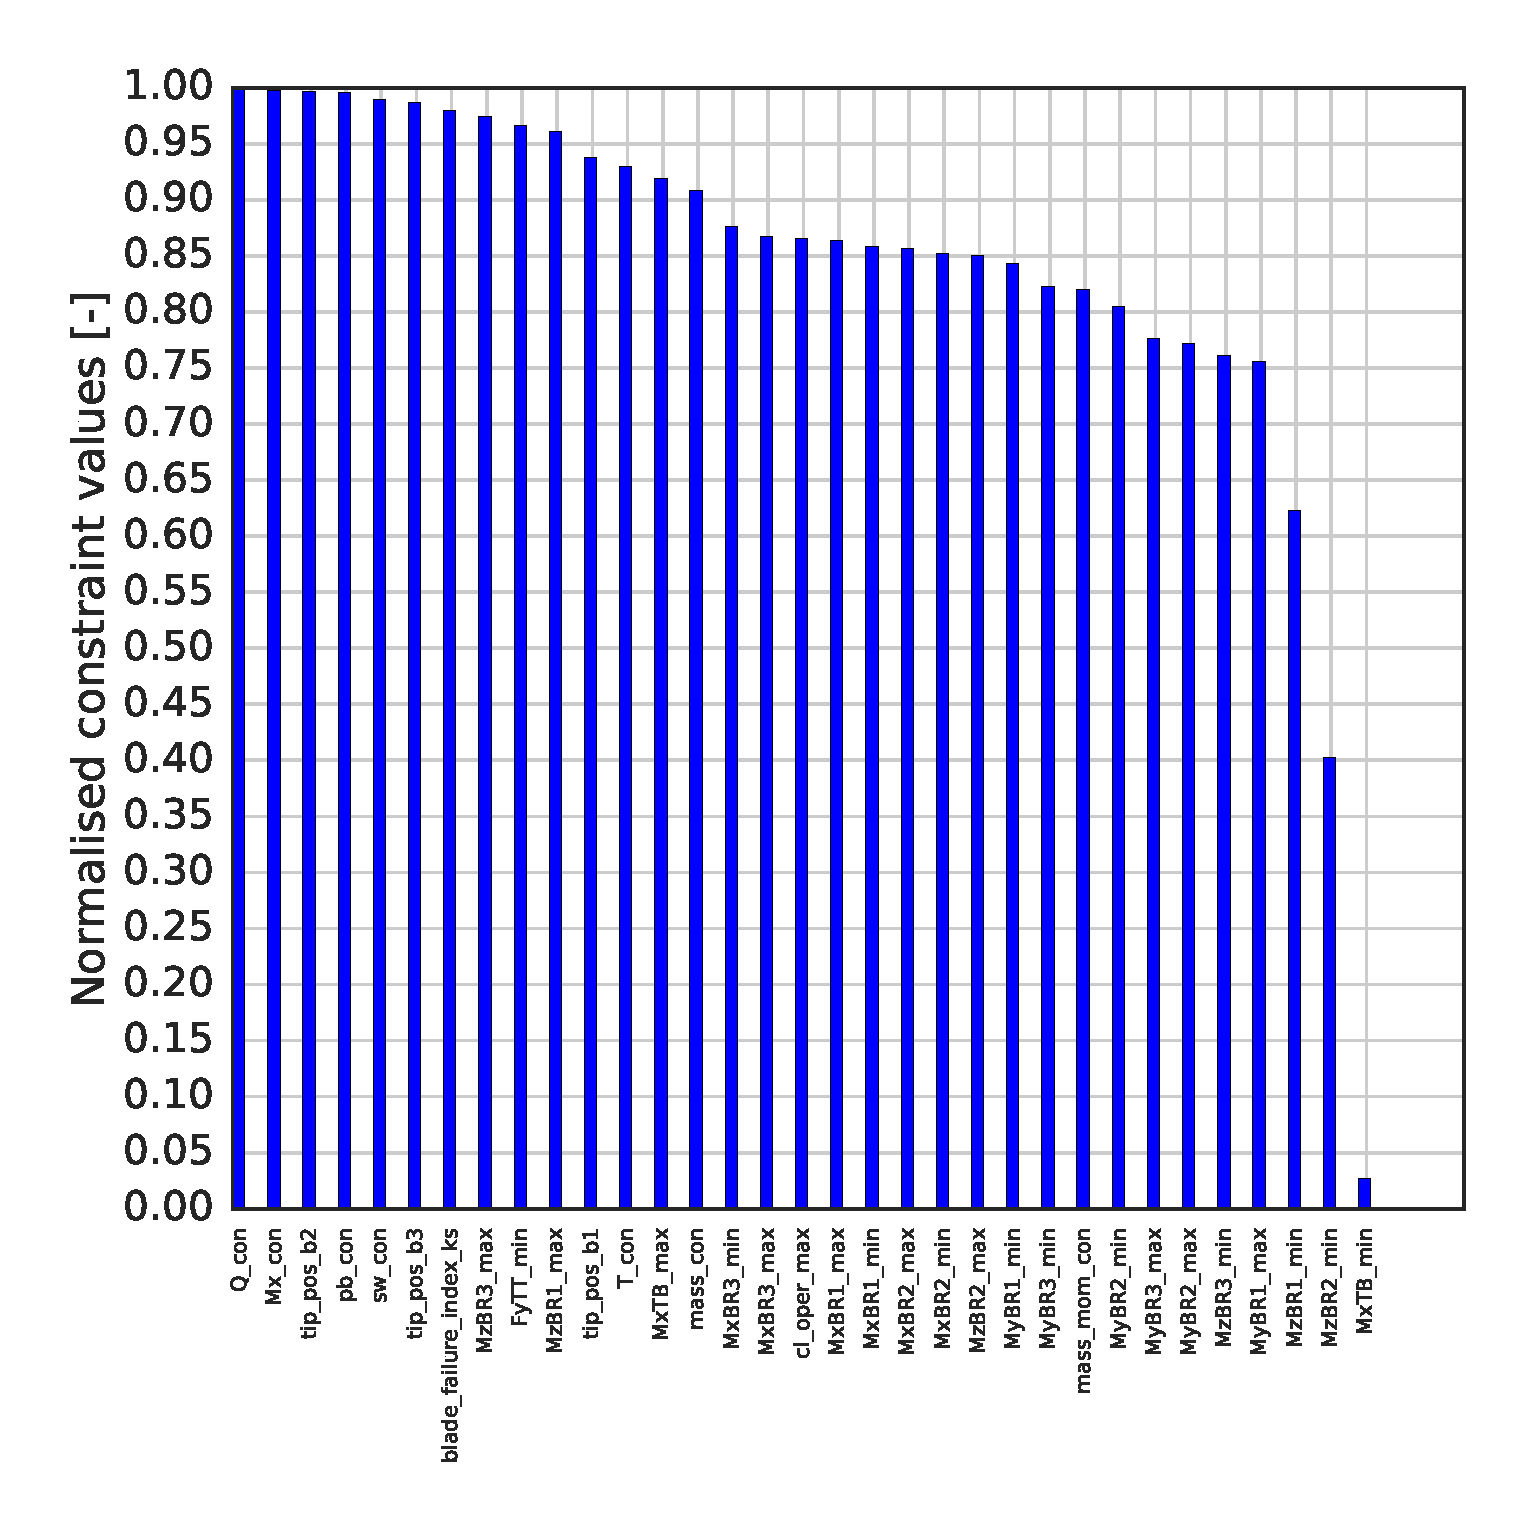
\includegraphics[width=.85\linewidth]{figures/KB6_final/KB6_cons_list.eps}
\end{center}
\caption{Normalised values of constraints depicting the main design drivers.}
\label{fig:KB6_cons}
\end{figure}



%\begin{figure}[tph]
%\begin{subfigure}{0.50\textwidth}
%\includegraphics[width=\linewidth]{./Chapter3/Aerodynamics/chord_finalsmth.eps}
%\caption{Chord distribution}
%\label{ch3:subfig:chord}
%\end{subfigure}
% ~
%\begin{subfigure}{0.50\textwidth}
%\includegraphics[width=\linewidth]{figures/KB6_final/.eps}
%\caption{Twist distribution}
%\label{ch3:subfig:twist}
%\end{subfigure}
%\caption{Blade planform properties}
%\label{ch3:fig:blade_geom}
%\end{figure}

\subsection{Planform}
The planform of the KB6 swept blade is compared to the reference blade in Figure \ref{fig:KB6_blade_geom} and Figure \ref{fig:KB6_sweep_prebend}. The chord length is seen to have decreased from the reference, as seen in Figure \ref{subfig:KB6_chord}. The reduction is greatest in the mid-span region of the blade. Additionally, the relative thickness of the blade sections have increased from the reference in the mid-span region. The decreased chord and increased relative thickness indicate a much slender blade profile than the reference. The twist angle is seen to increase in Figure \ref{subfig:KB6_twist}. It should be noted that the twist plotted in this figure, follows the right hand thumb rule convention for a z-coordinate axis that starts at the root and ends at the tip. Accordingly, it is regarded negative towards feather and positive towards stall. The twist in the KB6 blade has decreased compared to the reference case and is twisting less towards feather. This is to accommodate an increased tip-speed ratio of operation and the consequences of a slender blade design which has altered the angle of attack for which the airfoils can operate optimally. It is also observed from Figure \ref{subfig:KB6_twist} that difference between the twist angles of KB6 and the reference increase further in the last 20-25\% of the blade. This is due to the additional effect of torsion arising as a consequence of the geometric bend-twist coupling, to reduce the angle of attack by twisting towards feather. As such the pre-twist attains less negative values to compensate for this effect and to allow the airfoils in the affected region to operate optimally.


% planform figures 
\begin{figure}[tph]
\begin{subfigure}{0.50\textwidth}
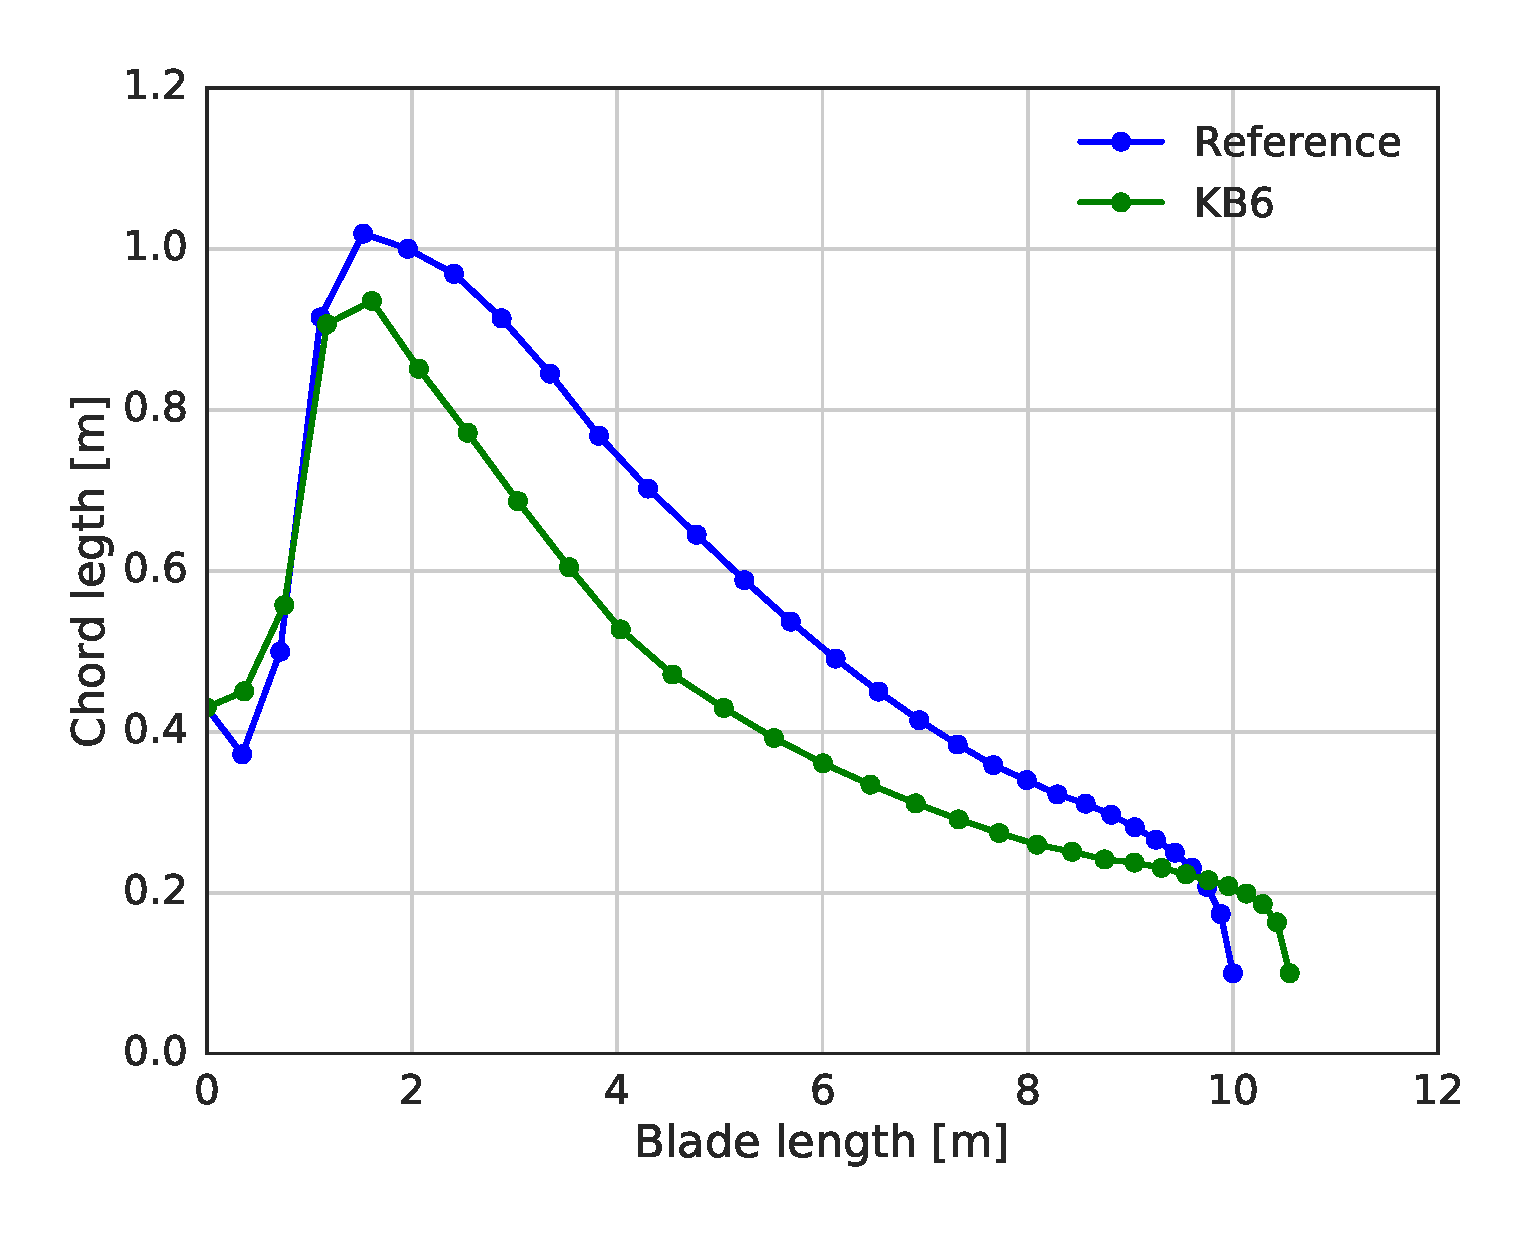
\includegraphics[width=\linewidth]{figures/KB6_final/KB6_chord.eps}
\caption{Chord distribution}
\label{subfig:KB6_chord}
\end{subfigure}
 ~
\begin{subfigure}{0.50\textwidth}
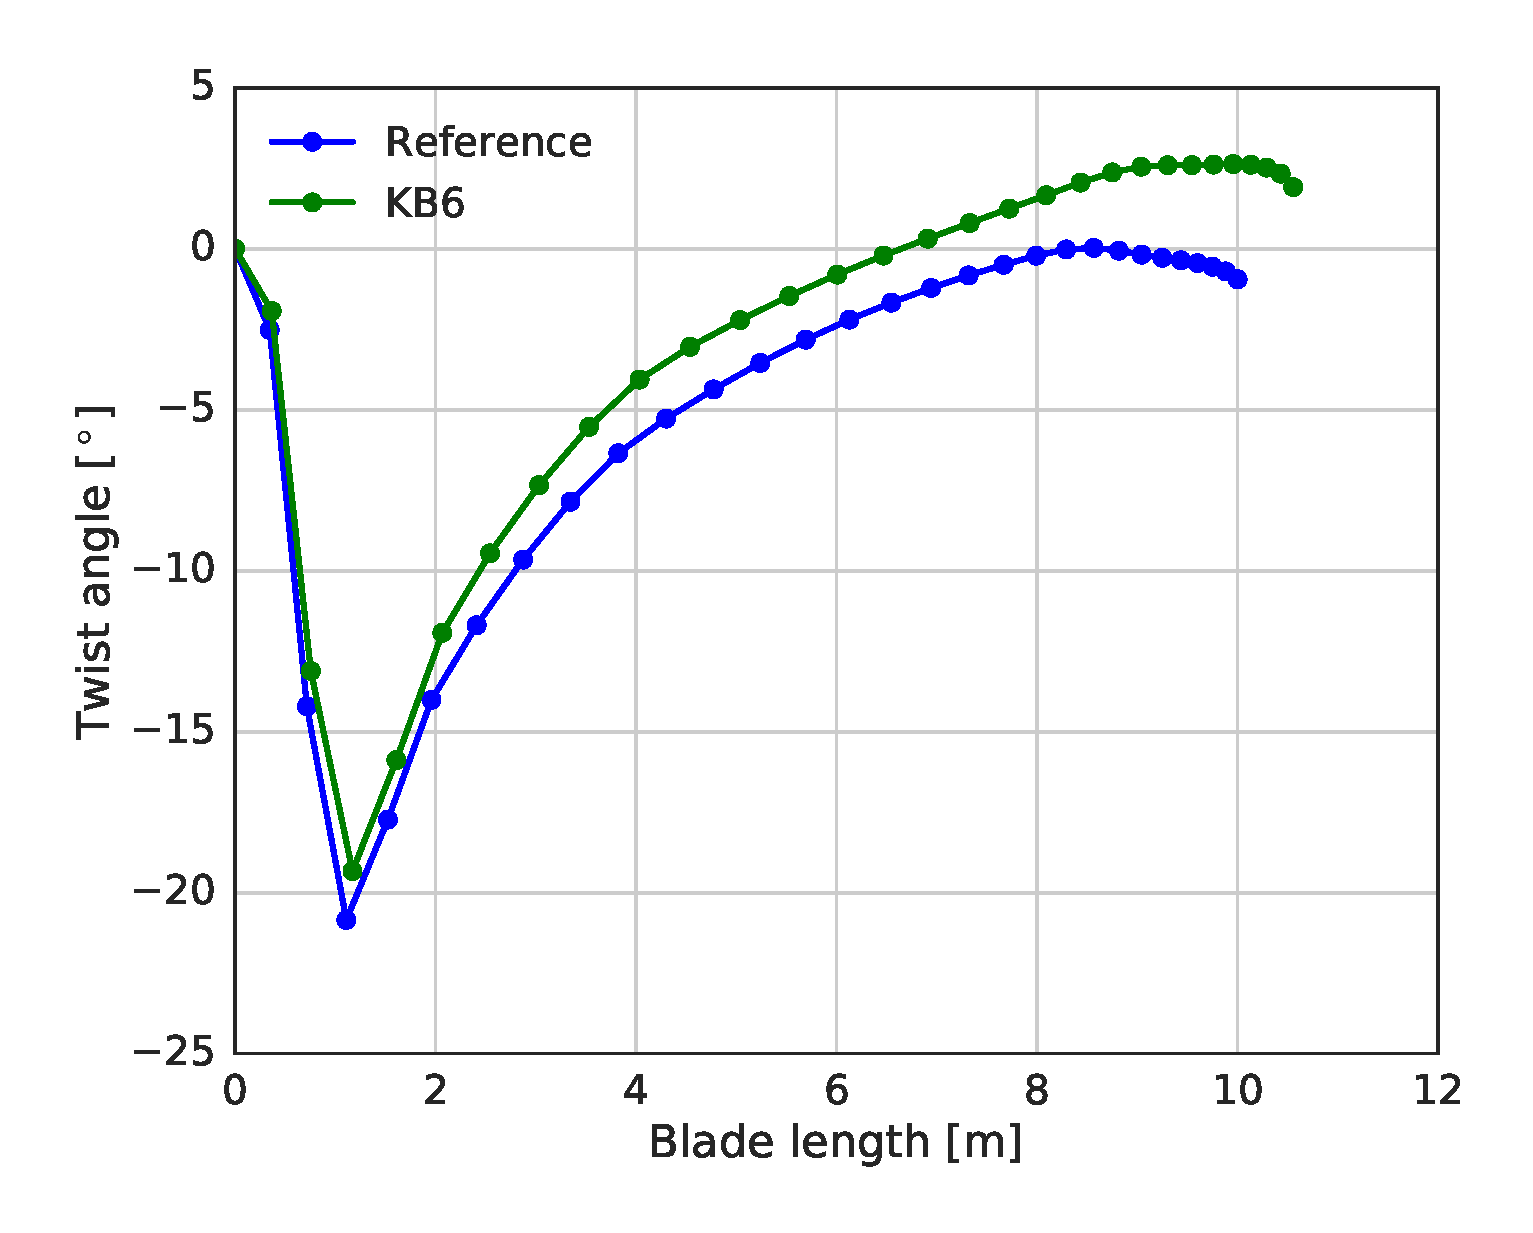
\includegraphics[width=\linewidth]{figures/KB6_final/KB6_twist.eps}
\caption{Twist distribution}
\label{subfig:KB6_twist}
\end{subfigure}

\begin{subfigure}{0.50\textwidth}
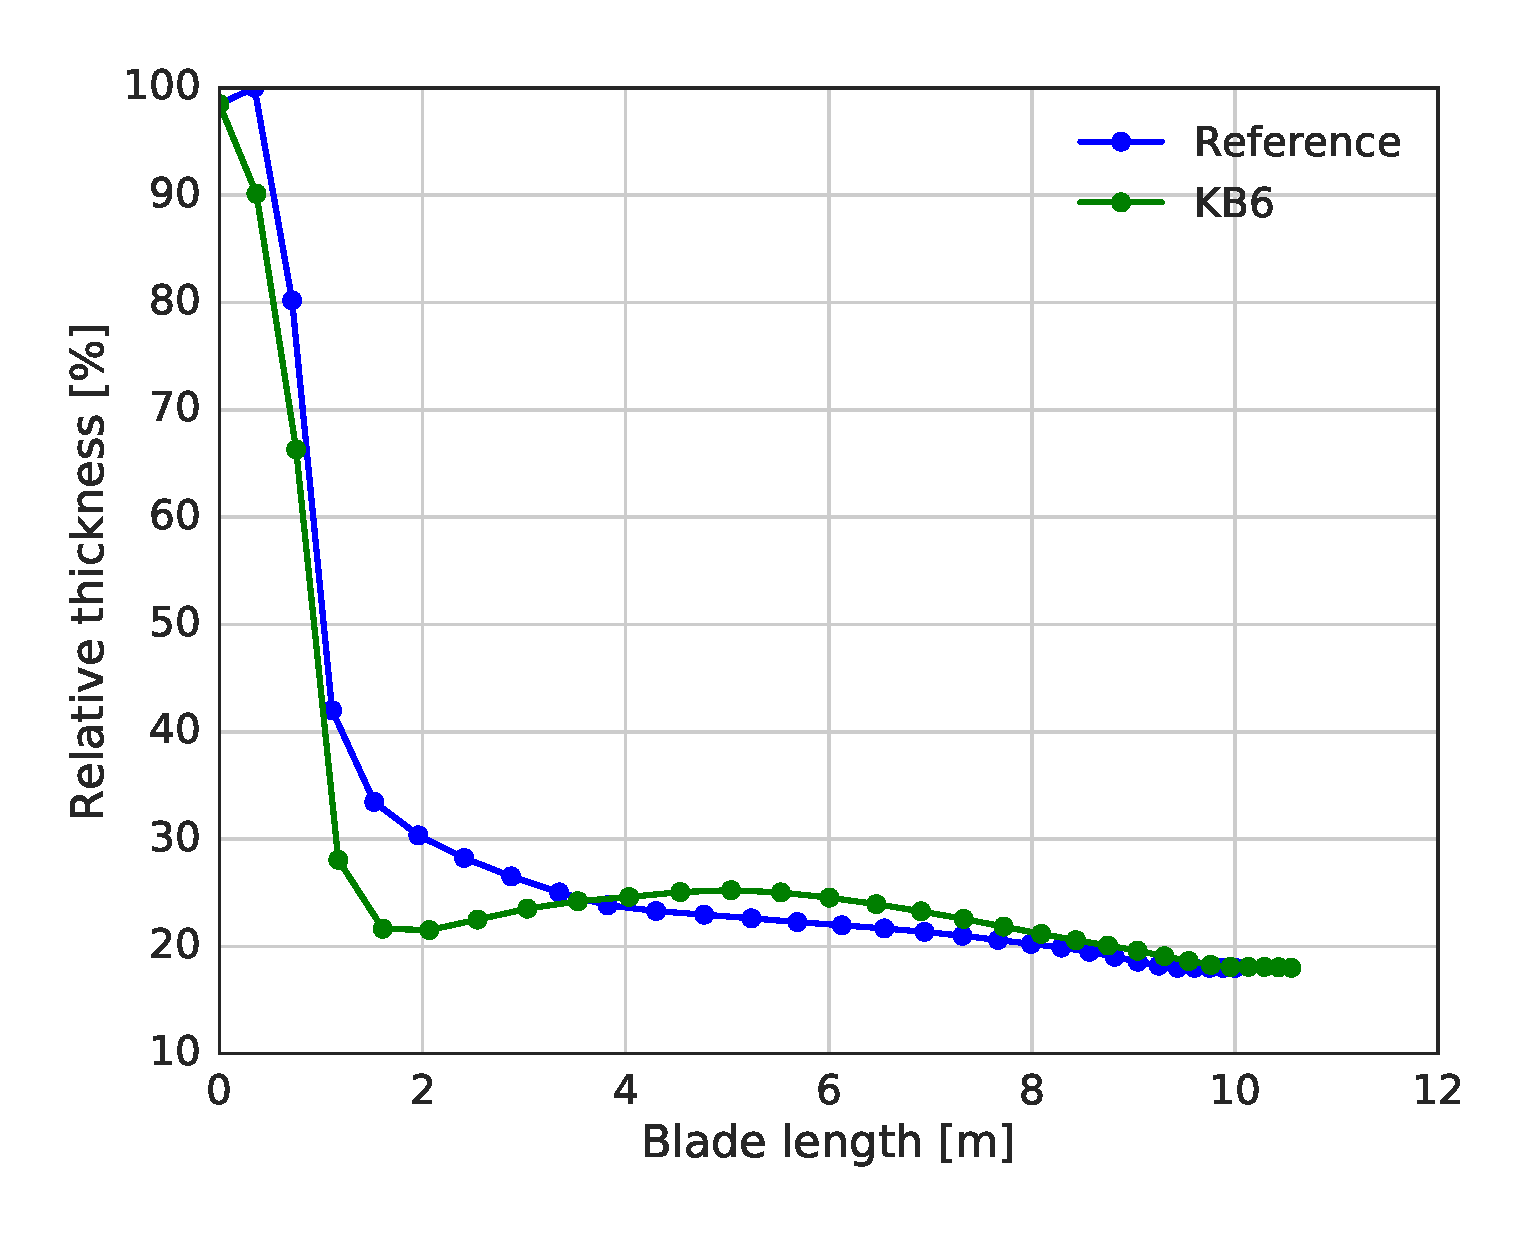
\includegraphics[width=\linewidth]{figures/KB6_final/KB6_rthick.eps}
\caption{Relative thickness distribution}
\label{subfig:KB6_rthick}
\end{subfigure}
 ~
\begin{subfigure}{0.50\textwidth}
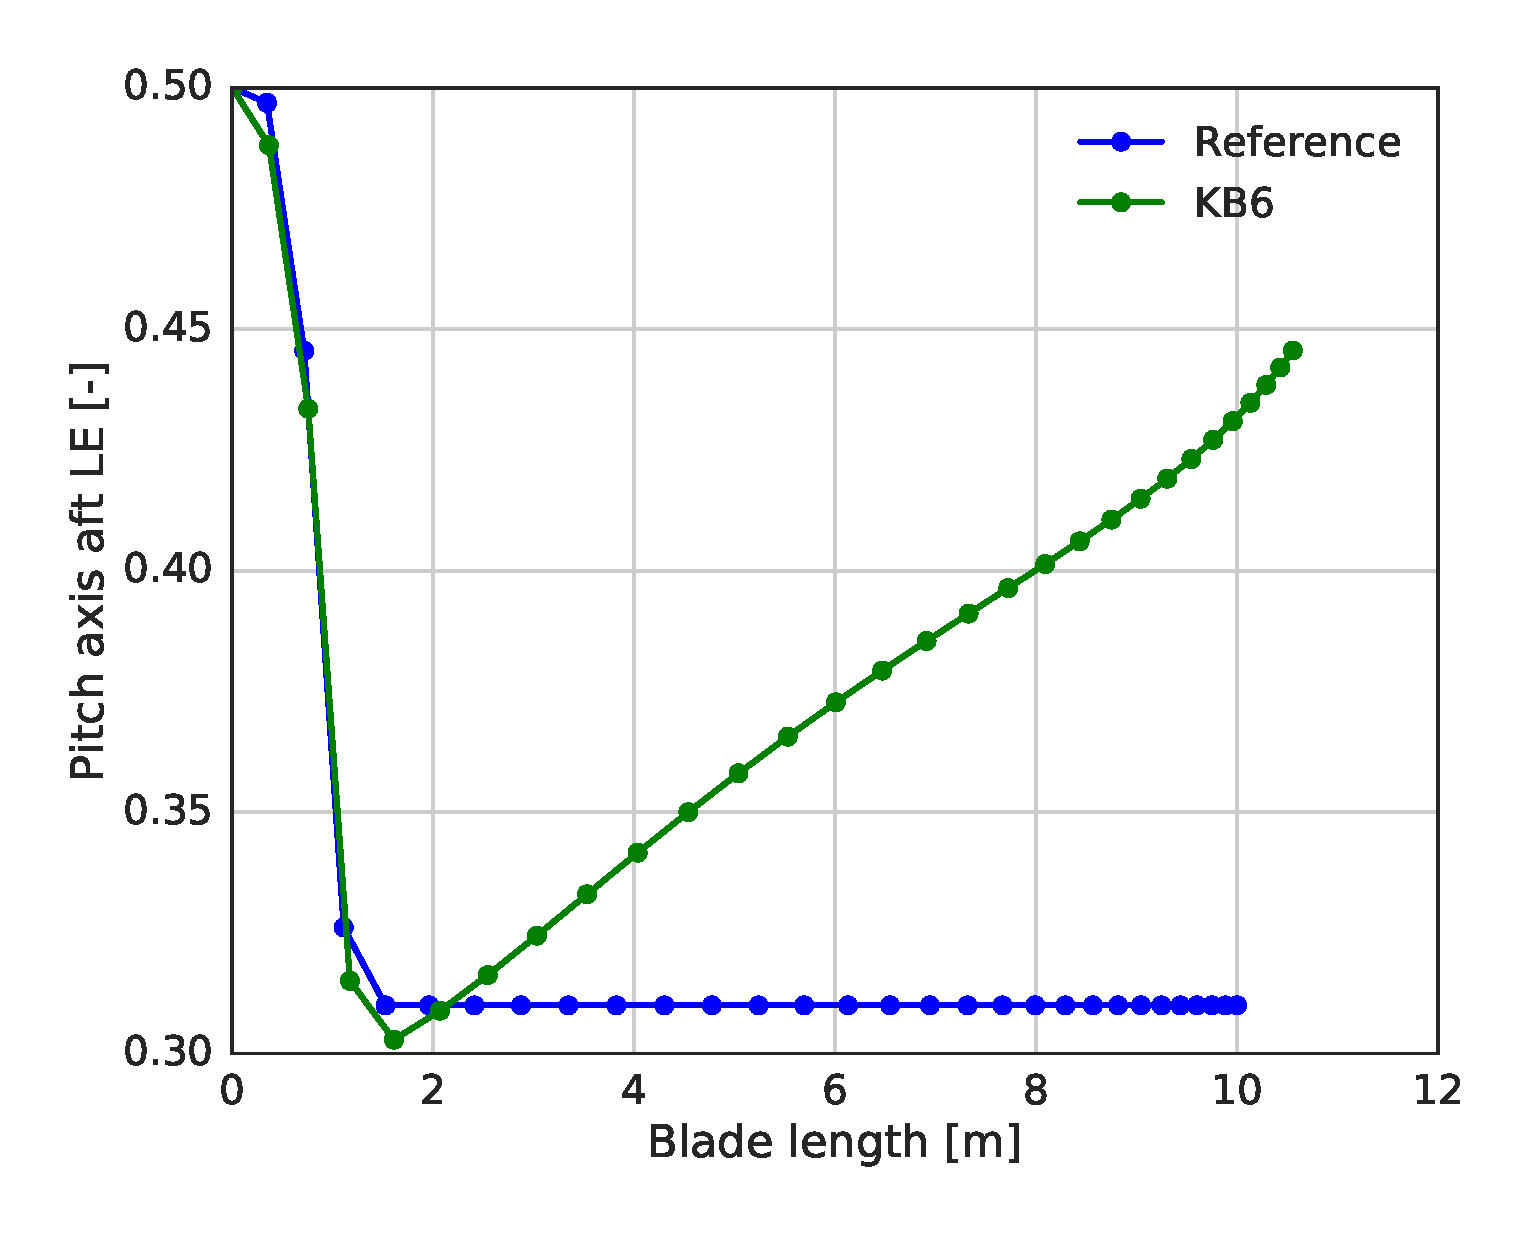
\includegraphics[width=\linewidth]{figures/KB6_final/KB6_ple.eps}
\caption{Pitch axis aft leading edge distribution}
\label{subfig:KB6_ple}
\end{subfigure}

\caption{Blade planform properties}
\label{fig:KB6_blade_geom}
\end{figure}

% sweep and prebend

\begin{figure}[tph]
\begin{subfigure}{0.50\textwidth}
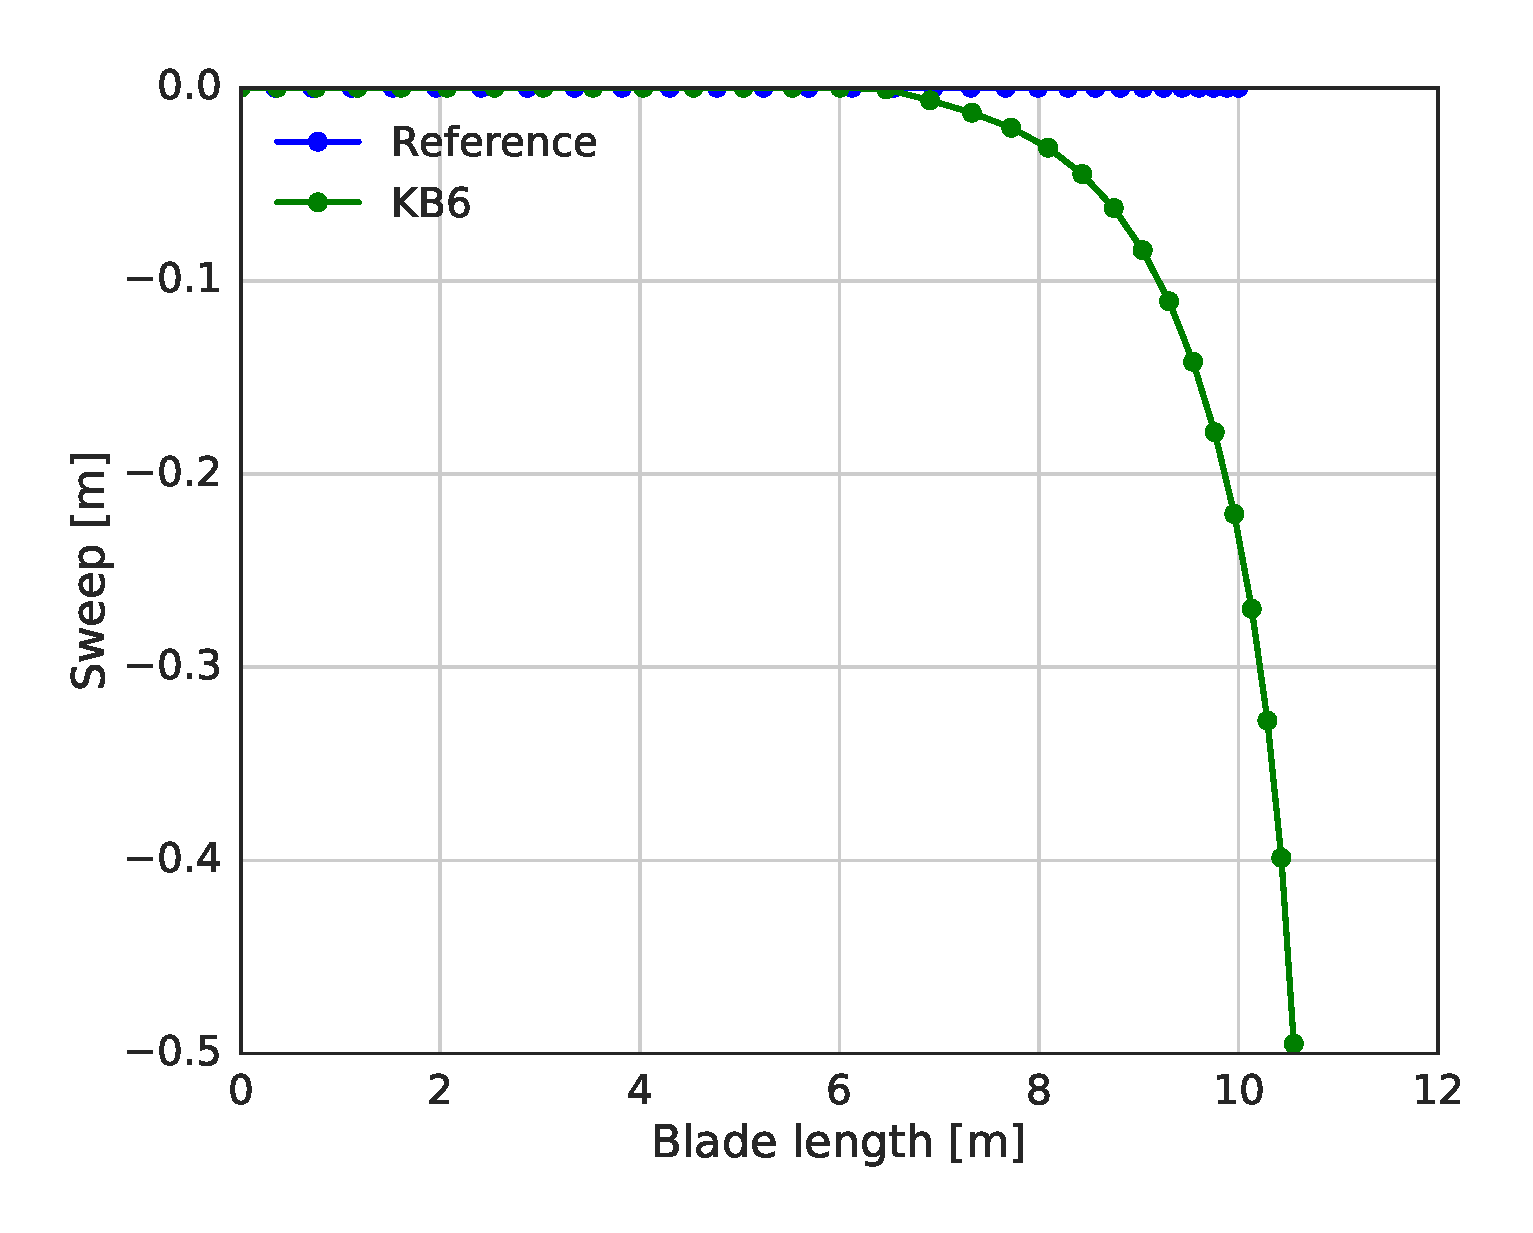
\includegraphics[width=\linewidth]{figures/KB6_final/KB6_sweep.eps}
\caption{Sweep distribution}
\label{subfig:KB6_sweep}
\end{subfigure}
 ~
\begin{subfigure}{0.50\textwidth}
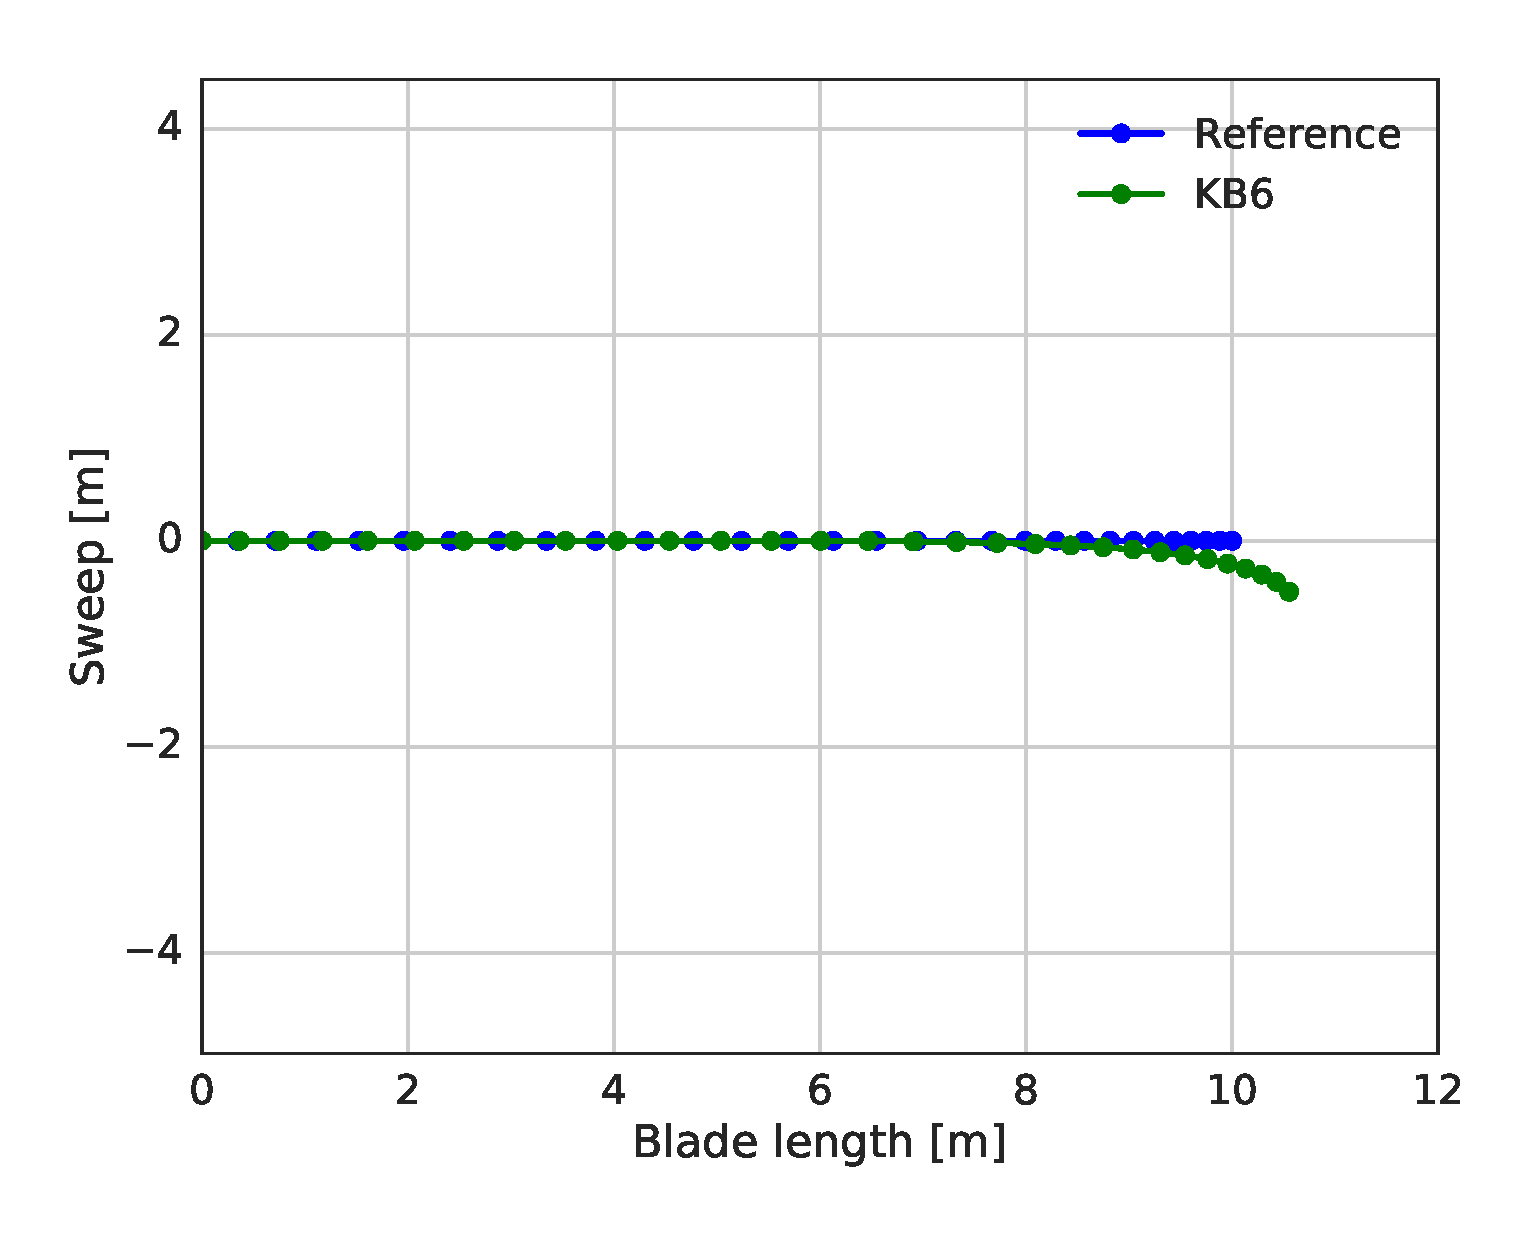
\includegraphics[width=\linewidth]{figures/KB6_final/KB6_sweep_scale.eps}
\caption{Sweep distribution to scale}
\label{subfig:KB6_sweep_scale}
\end{subfigure}

\begin{subfigure}{0.50\textwidth}
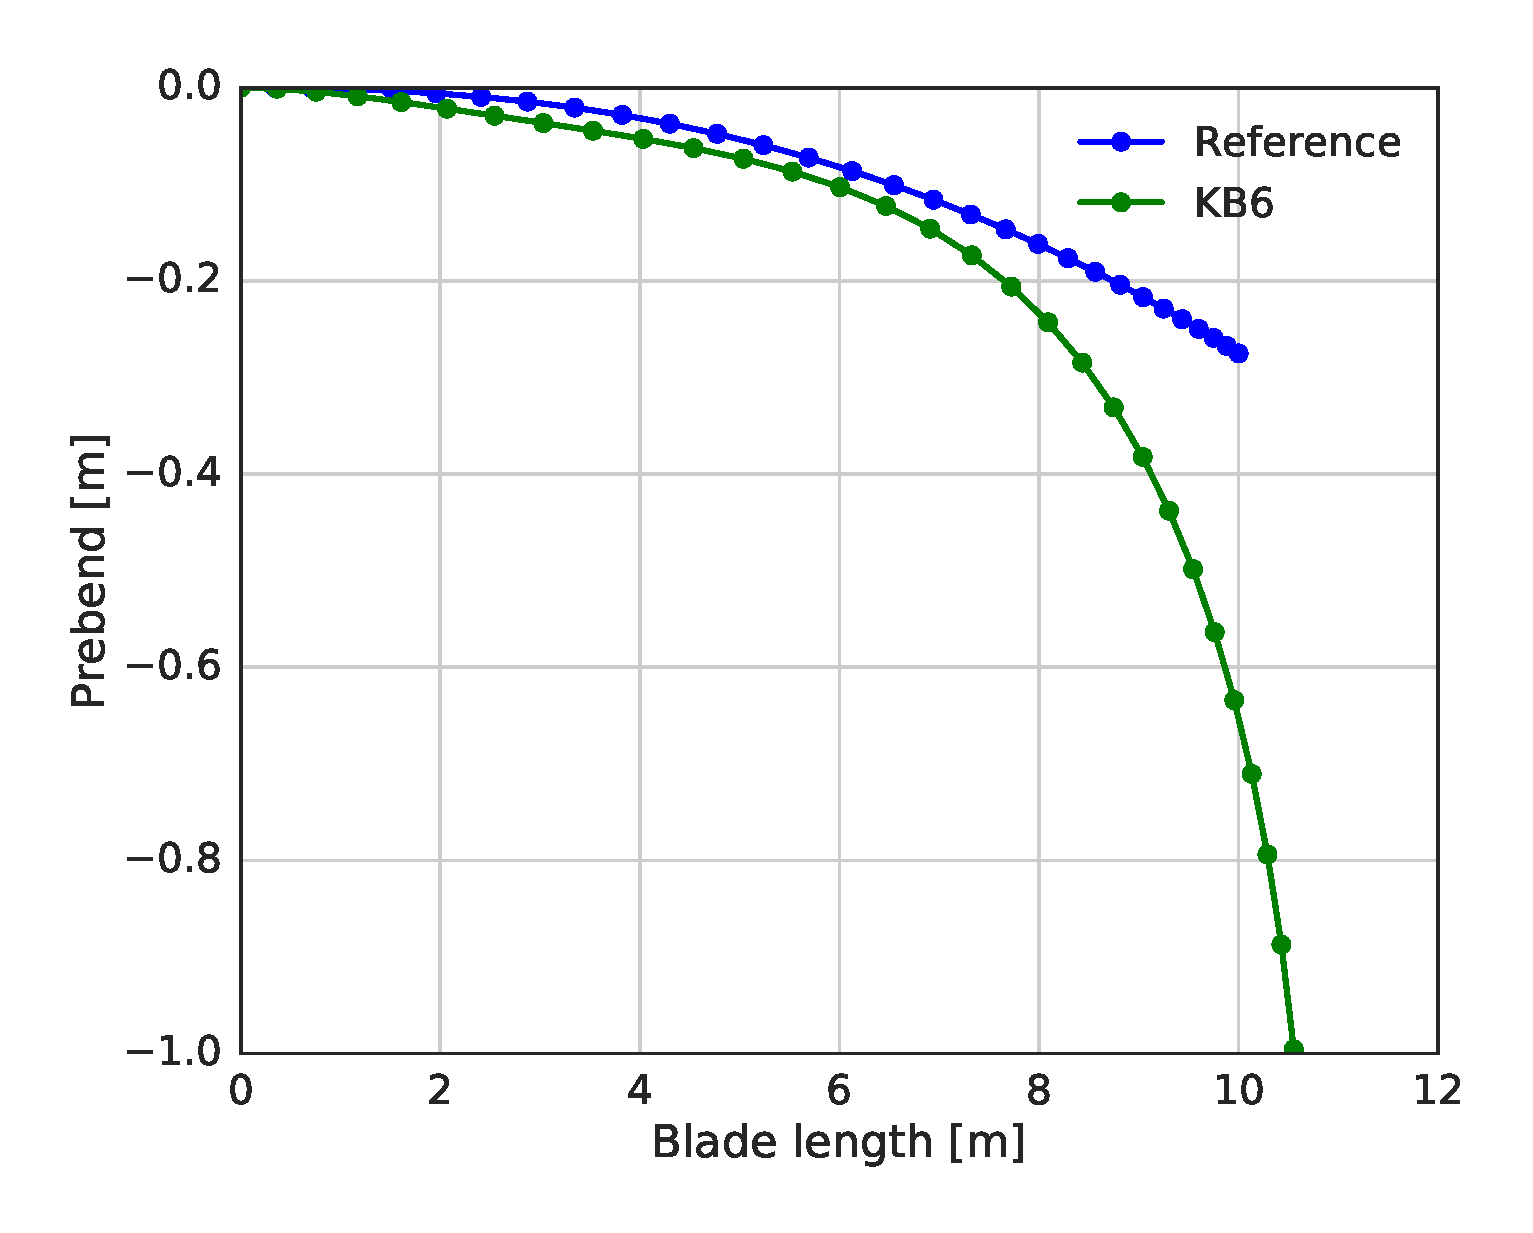
\includegraphics[width=\linewidth]{figures/KB6_final/KB6_prebend.eps}
\caption{Prebend distribution}
\label{subfig:KB6_prebend}
\end{subfigure}
 ~
\begin{subfigure}{0.50\textwidth}
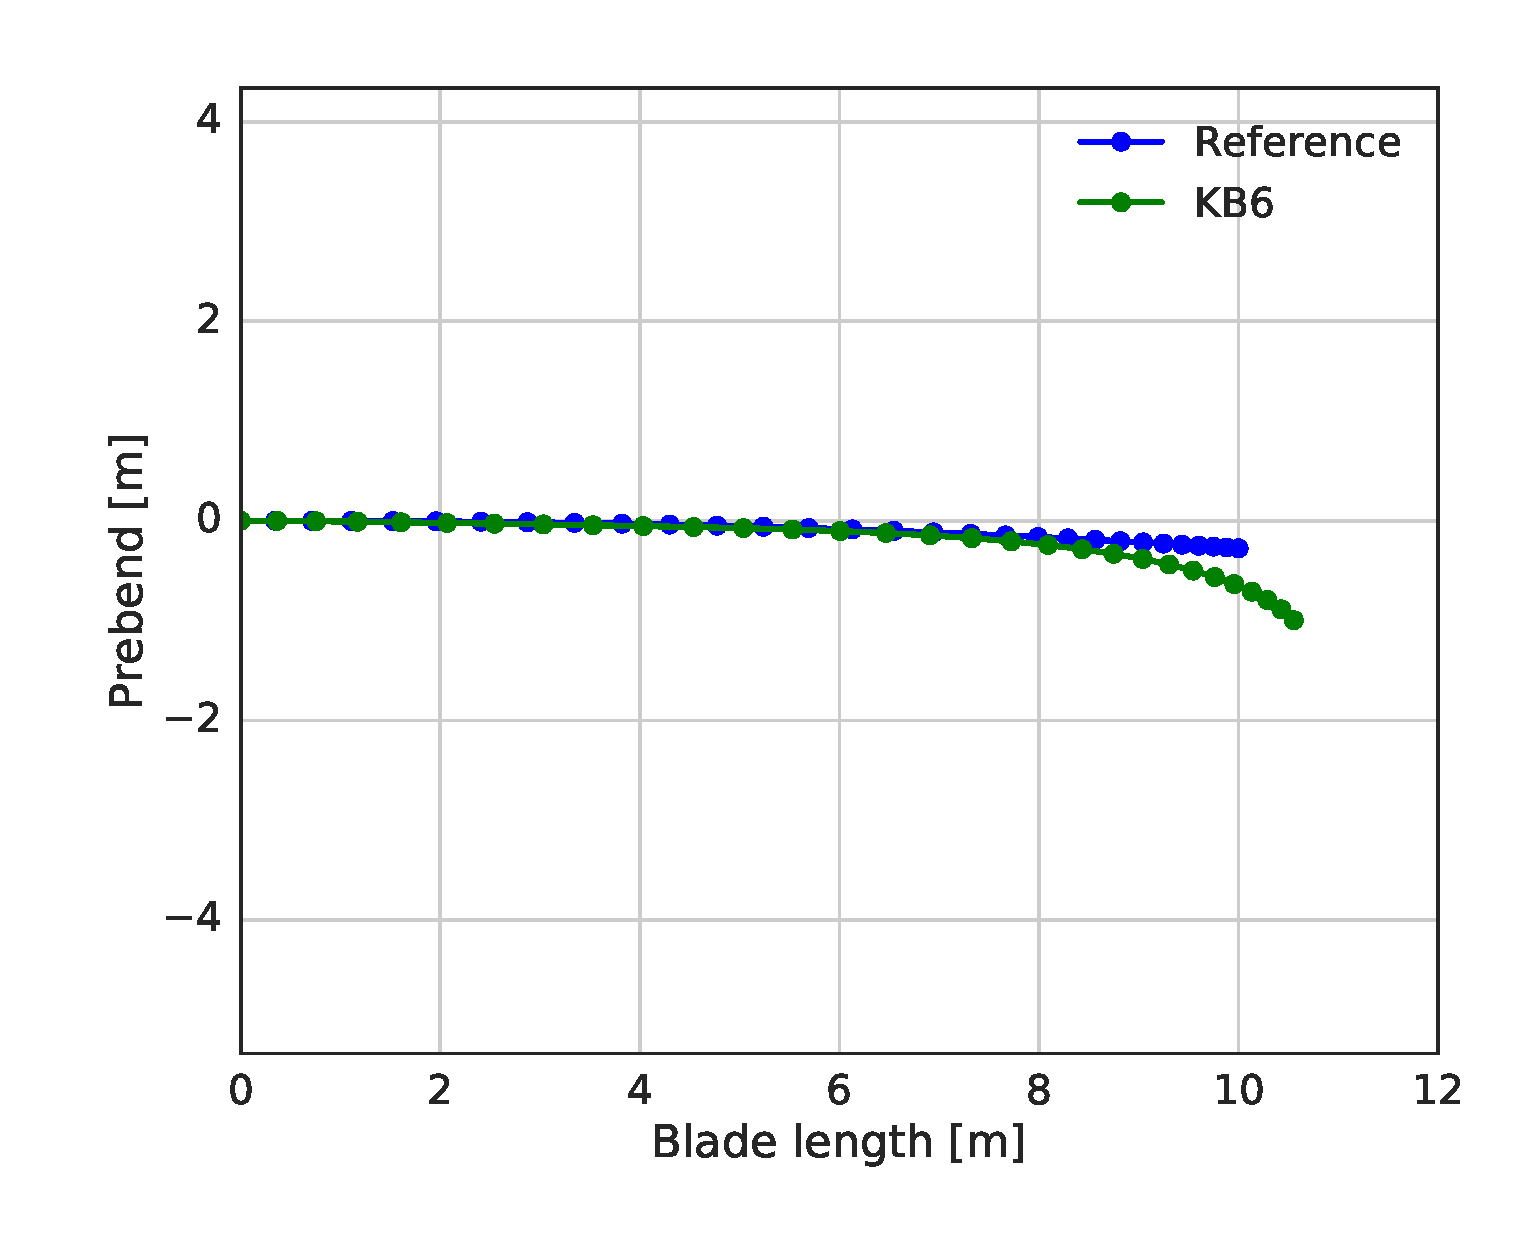
\includegraphics[width=\linewidth]{figures/KB6_final/KB6_prebend_scale.eps}
\caption{Prebend distribution to scale}
\label{subfig:KB6_prebend_scale}
\end{subfigure}

\caption{Blade planform properties}
\label{fig:KB6_sweep_prebend}
\end{figure}

\subsection{Structure}
\label{subsec:KB6_structure}

\subsubsection*{Composite layup}
The material layup in the various regions of the blade sections along with the corresponding laminate thicknesses are shown in Figures \ref{fig:KB6_mat_r01} to \ref{fig:KB6_mat_r07}. The two outer triax layers remain unchanged while the rest of the internal layers are afforded design freedom during the optimization and vary according to the solution. 

Figure \ref{fig:KB6_mat_r01} shows the material information in the trailing edge reinforcement of the blade. Referring to the blade cross-section shown in Figure \ref{fig:cross_section_def}, this region is between the points DP00 and DP02 on the pressure side and between DP15 and DP17 on the suction side. It is seen that compared to the reference the KB6 blade has a greater thickness in this region especially near the root. This has been carried out by adding more uniax material.

Figure \ref{fig:KB6_mat_r02} depicts the material layup in the main panel of the blade which is situated between the spar cap and trailing edge reinforcement. In Figure \ref{fig:cross_section_def} showing the cross-section information, this region lies between the points DP02 and DP04 on the pressure side and between DP13 and DP15 on the suction side. In this region the laminate thicknesses are mostly similar to the reference blade. Except near the root it is less thicker. This has been done by reducing the uniax material. Similarly the thickness is greater from 20\% to 40\% blade length. This has been facilitated by increasing the triax material in the layup. 

Figure \ref{fig:KB6_mat_r04} presents the material layup in the spar cap of the blade. From Figure \ref{fig:cross_section_def} it is seen that this region lies between the points DP04 and DP07 on the pressure side and between DP10 and DP13 on the suction side. The thickness of the laminate from 40\% span to 90\% span has been reduced considerably, by a factor of two on average. At the same time, the thickness between the root and around 30\% span has increased compared to the reference. This has been mainly done by altering the uniax material. Two thin layers of triax have also been added.

Figure \ref{fig:KB6_mat_r06} shows the material distribution and laminate thickness in the leading region of the blade situated between the leading edge and the spar cap. On referring to Figure \ref{fig:cross_section_def} it is seen that this region lies between the points DP07 and DP08 on the pressure side and between the points DP09 and DP10 on the suction side of the blade section. The laminate thickness has been reduced in the KB6 bade in the near root region, while it has been slightly increased from 20\% to 40\% span. The reduction in the laminate thickness is due to the removal of the uniax layer near the root. Whereas a layer of triax has been added throughout the early span and is responsible for the increase in thickness from 20\% to 40\%span.

Figure \ref{fig:KB6_mat_r07} shows the material information in the leading edge reinforcement of the blade. From the cross-section shown in Figure \ref{fig:cross_section_def} it is seen that this region lies between the division points DP08 and DP09 and includes the leading edge. The laminate thickness has increased from the near root region until 50\% span. This increase is primarily due the addition of two triax layers. The thickness has also increased from around 70\% span until the tip. The increase here is attributed to the addition of uniax material in the layup. 

The material in the shear webs are not provided design freedom during the optimization and remain unchanged in thickness and material composition.

\subsubsection*{Blade stiffnesses}
Figure \ref{fig:KB6_stiffness} presents the flapwise, edgewise and torsional stiffnesses of the KB6 blade compared to the reference over a normalized span. All three stiffnesses are seen to have decreased for majority of the blade span except at the root and tip, which show a slight increase. This is a result of the reduction in the chord length in the KB6 blade compared to the reference as seen in Figure \ref{subfig:KB6_chord}. Cross-sectional stiffnesses in a thin composite laminate section scale to the cube of the local chord and scale directly with the laminate thickness. This dependence can be derived by applying classical laminate theory to a thin cross-section. The reader is directed to the ECN report by Kooijman \cite{kooijman1996bending} for the actual derivation. From the previous section it is seen that the laminate thicknesses too have been reduced considerably in the spar cap region, which is the structural entity that contributes the most towards cross-sectional stiffness. 


%%Material thickness and layup
%region 1
\begin{figure}[tph]
\begin{subfigure}{0.50\textwidth}
\centering
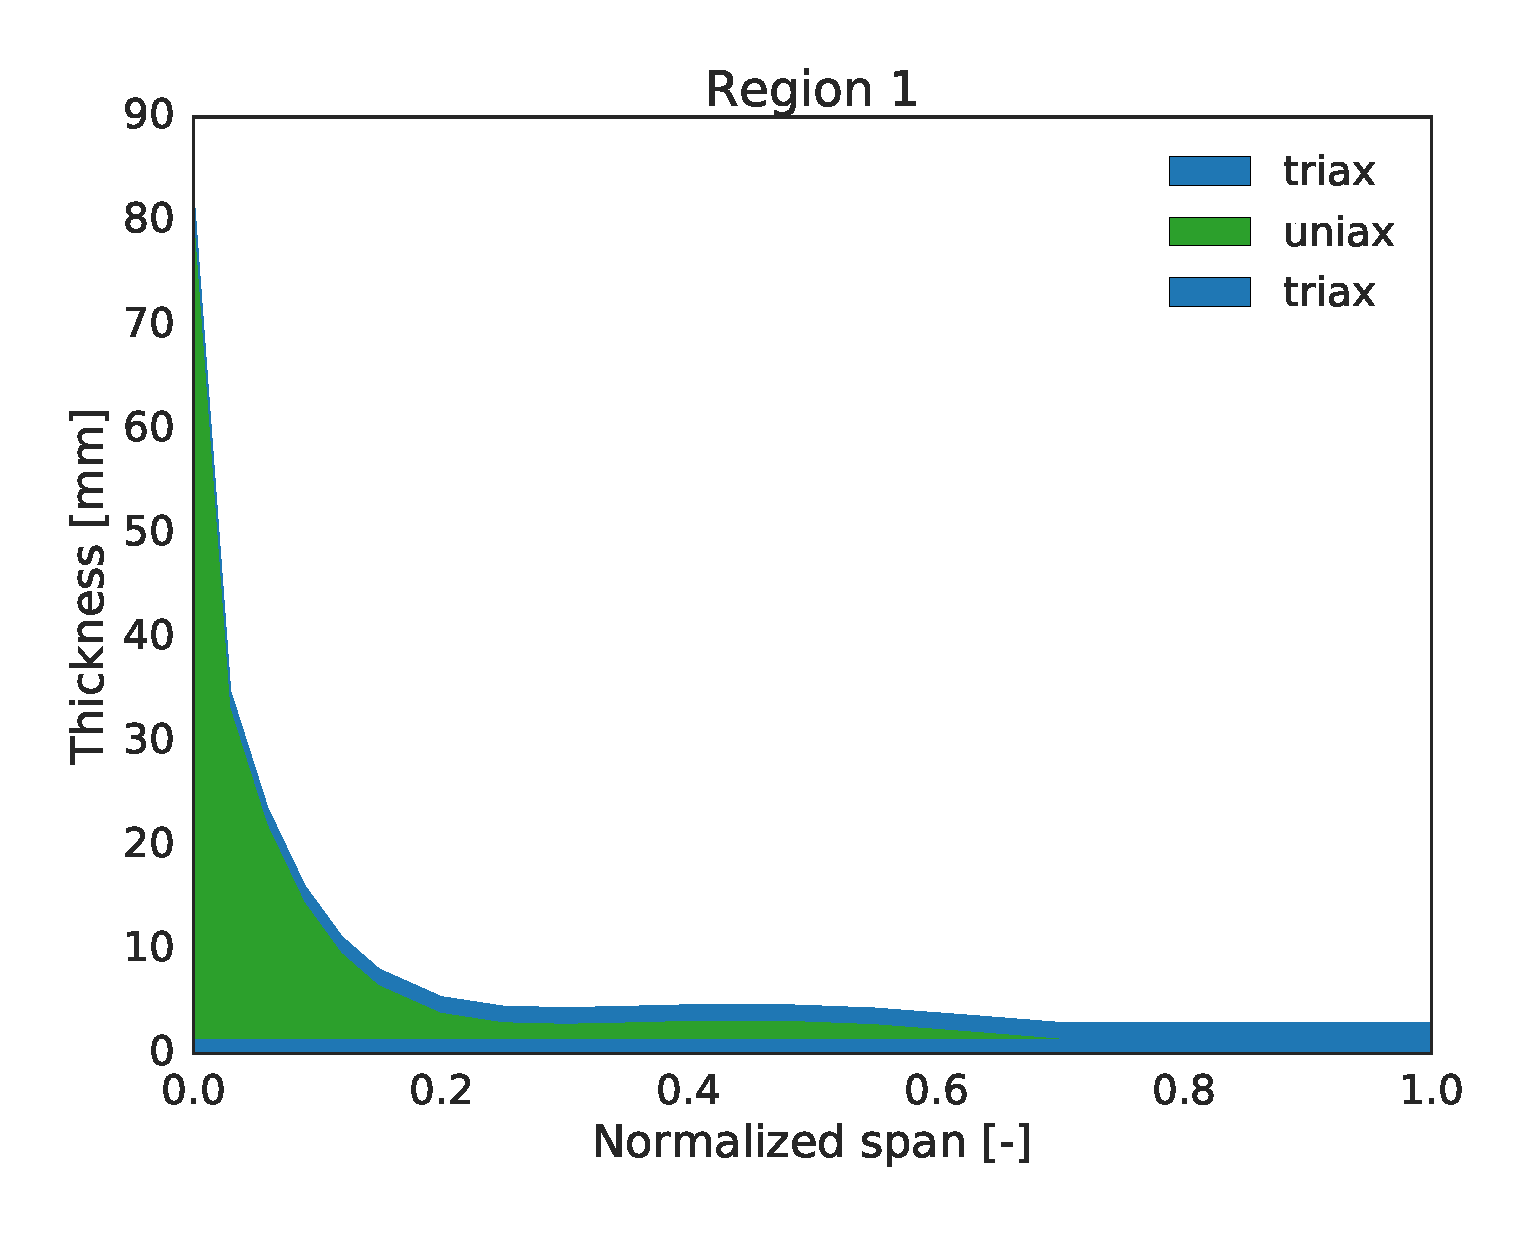
\includegraphics[width=\linewidth]{figures/KB6_final/baseline_laminate_layers_r01.eps}
\caption{Laminate layup of reference blade}
\label{subfig:baseline_layers_r01}
\end{subfigure}
 ~
\begin{subfigure}{0.50\textwidth}
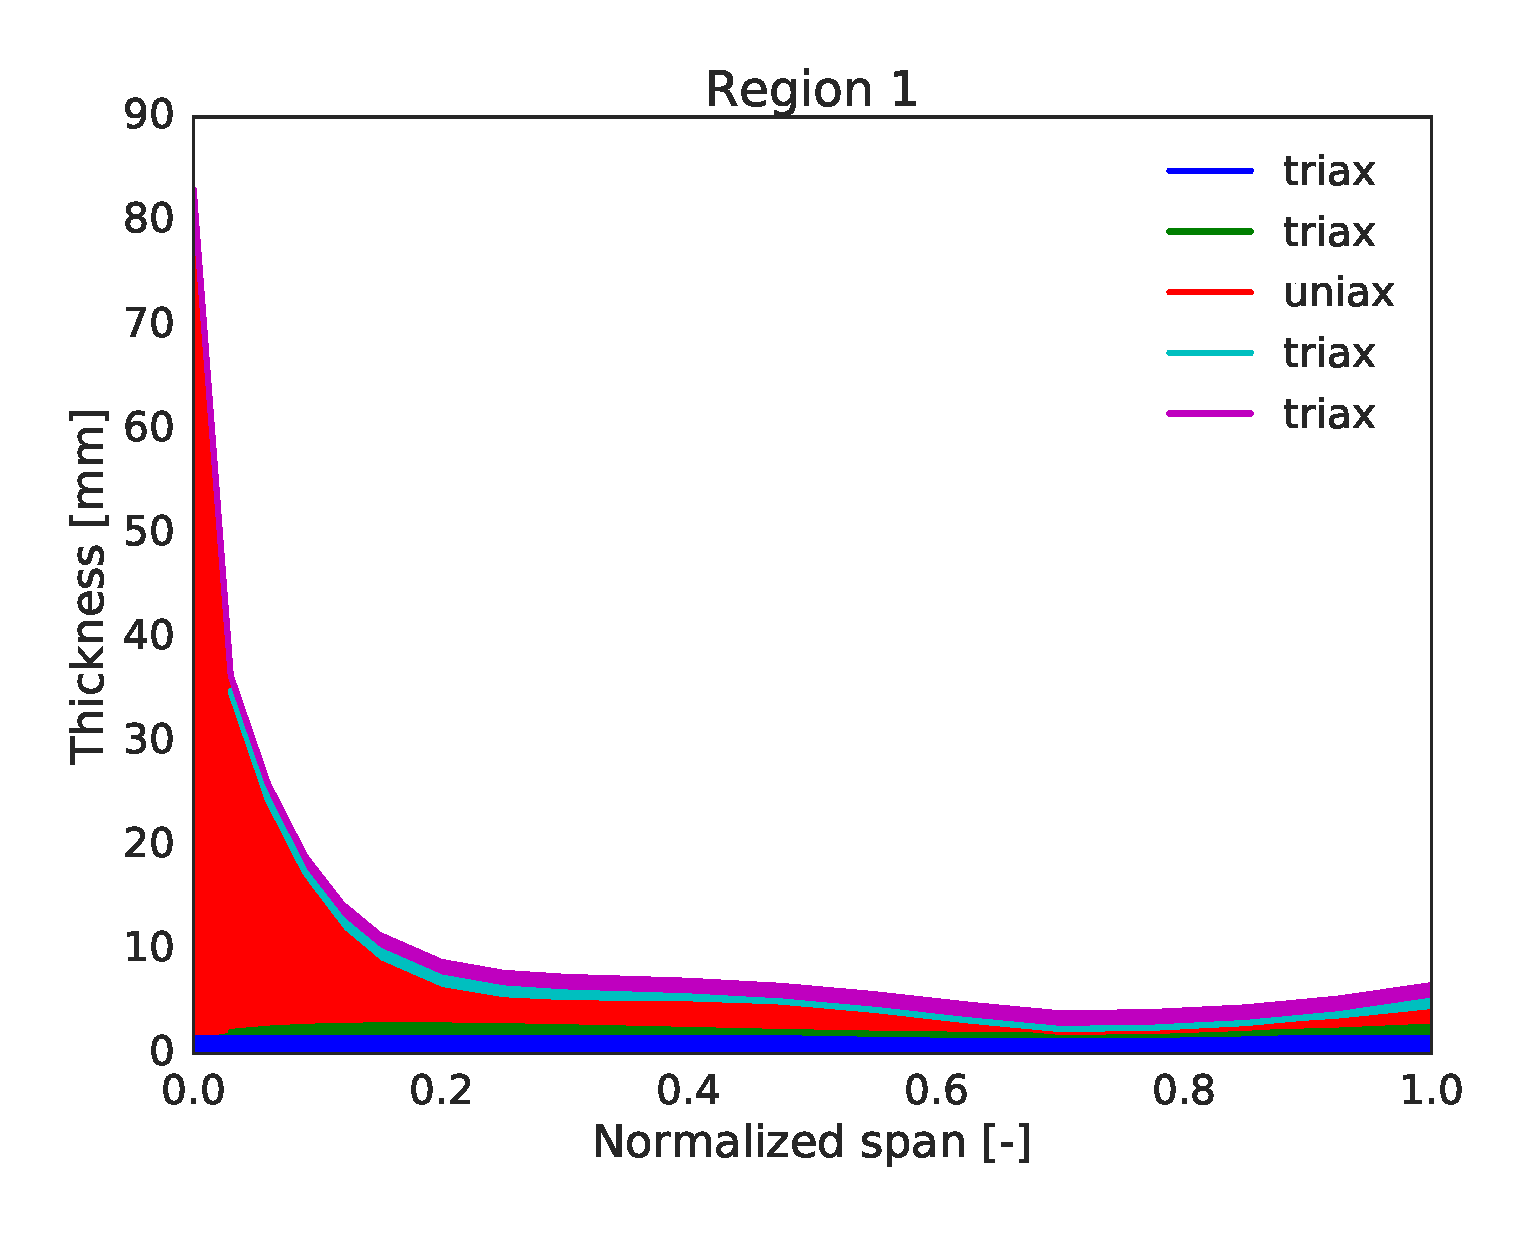
\includegraphics[width=\linewidth]{figures/KB6_final/KB6_laminate_layers_r01.eps}
\caption{Laminate layup of KB6 blade}
\label{subfig:KB6_layers_r01}
\end{subfigure}

\begin{subfigure}{\textwidth}
\centering
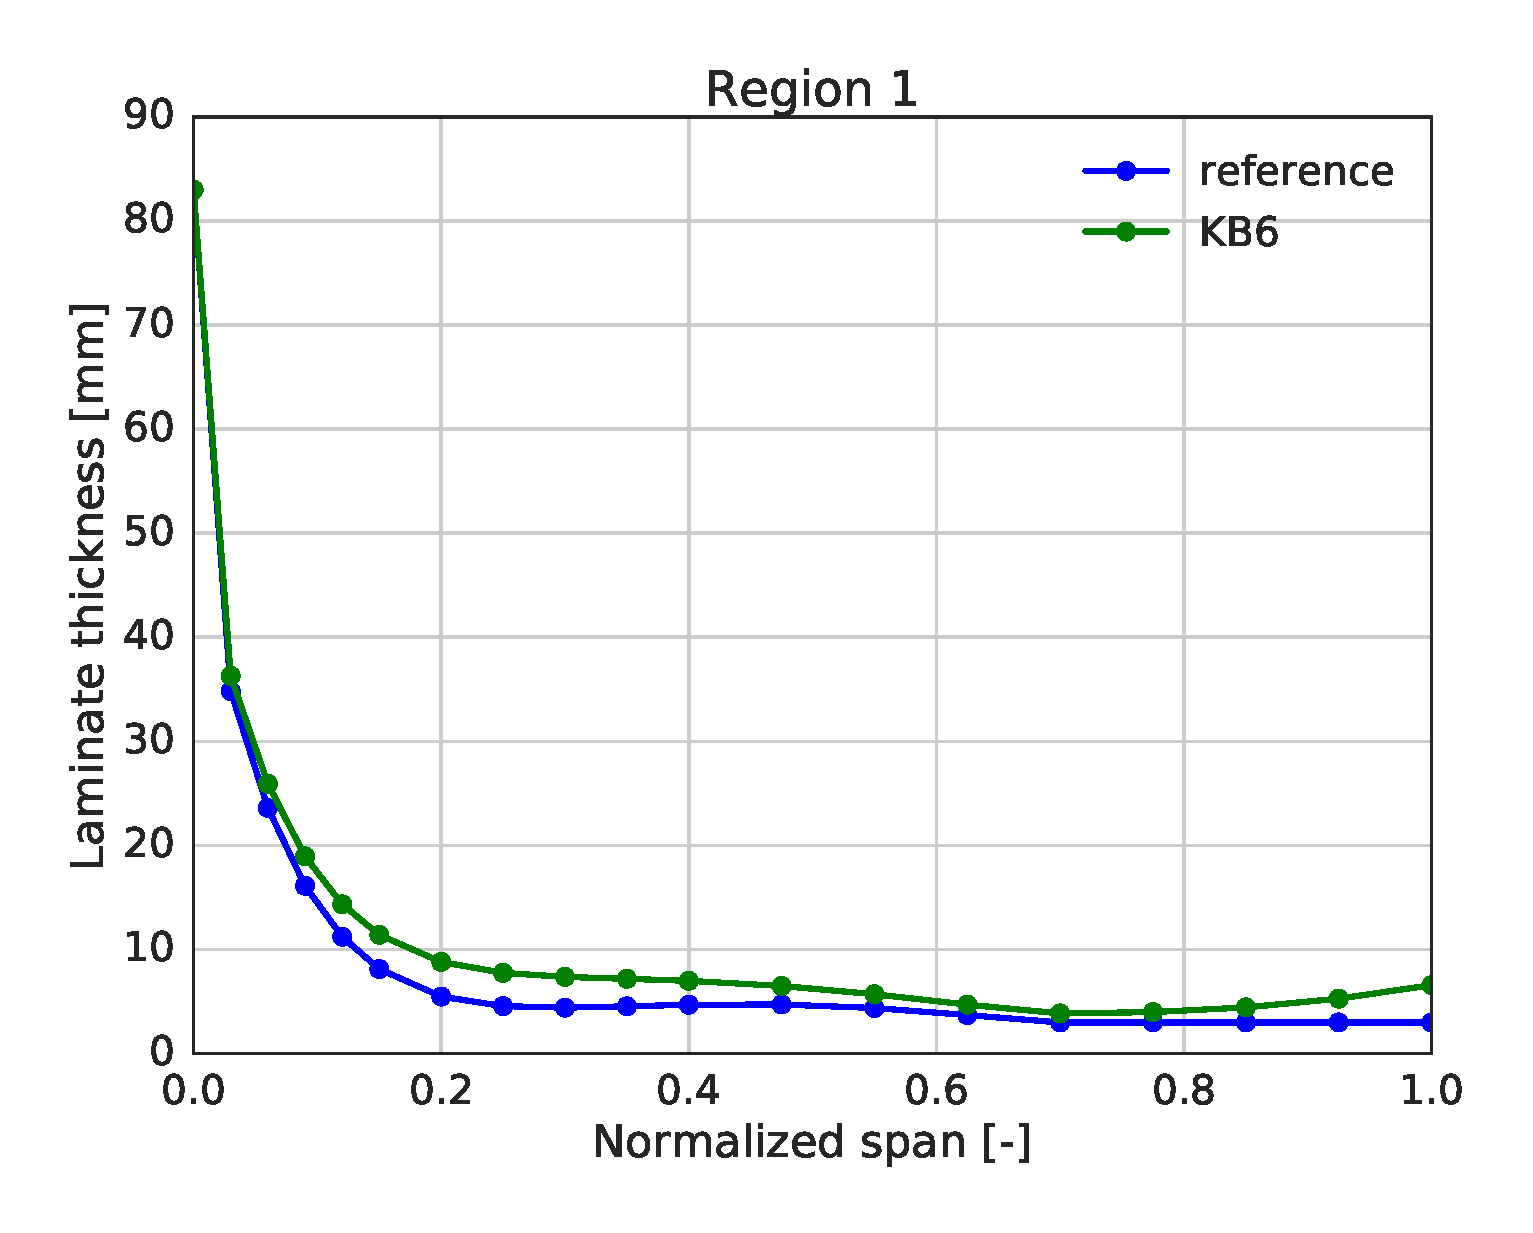
\includegraphics[width=0.50\linewidth]{figures/KB6_final/KB6_r01_thickness.eps}
\caption{Laminate thickness comparison of KB6 with reference}
\label{subfig:KB6_thick_r01}
\end{subfigure}
\caption{ Material in the trailing edge reinforcement}
\label{fig:KB6_mat_r01}
\end{figure}

%region 2
\begin{figure}[tph]
\begin{subfigure}{0.50\textwidth}
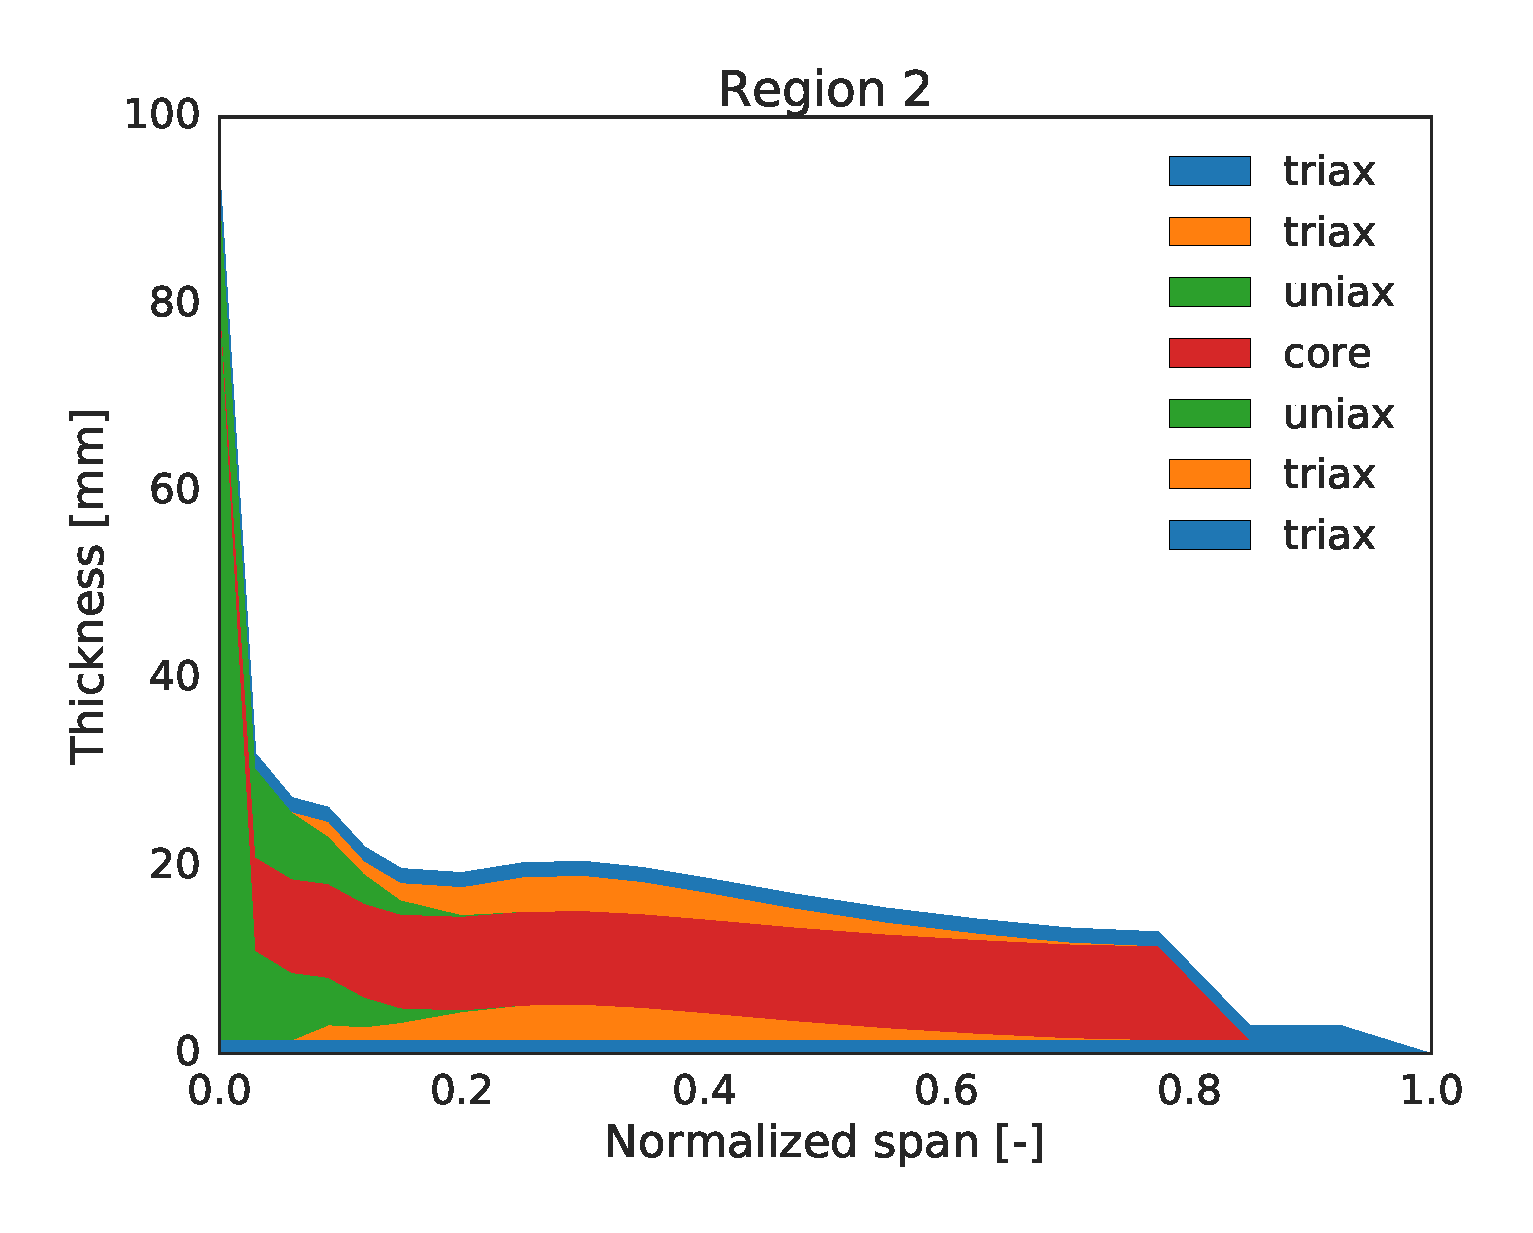
\includegraphics[width=\linewidth]{figures/KB6_final/baseline_laminate_layers_r02.eps}
\caption{Laminate layup of reference blade}
\label{subfig:baseline_layers_r02}
\end{subfigure}
 ~
\begin{subfigure}{0.50\textwidth}
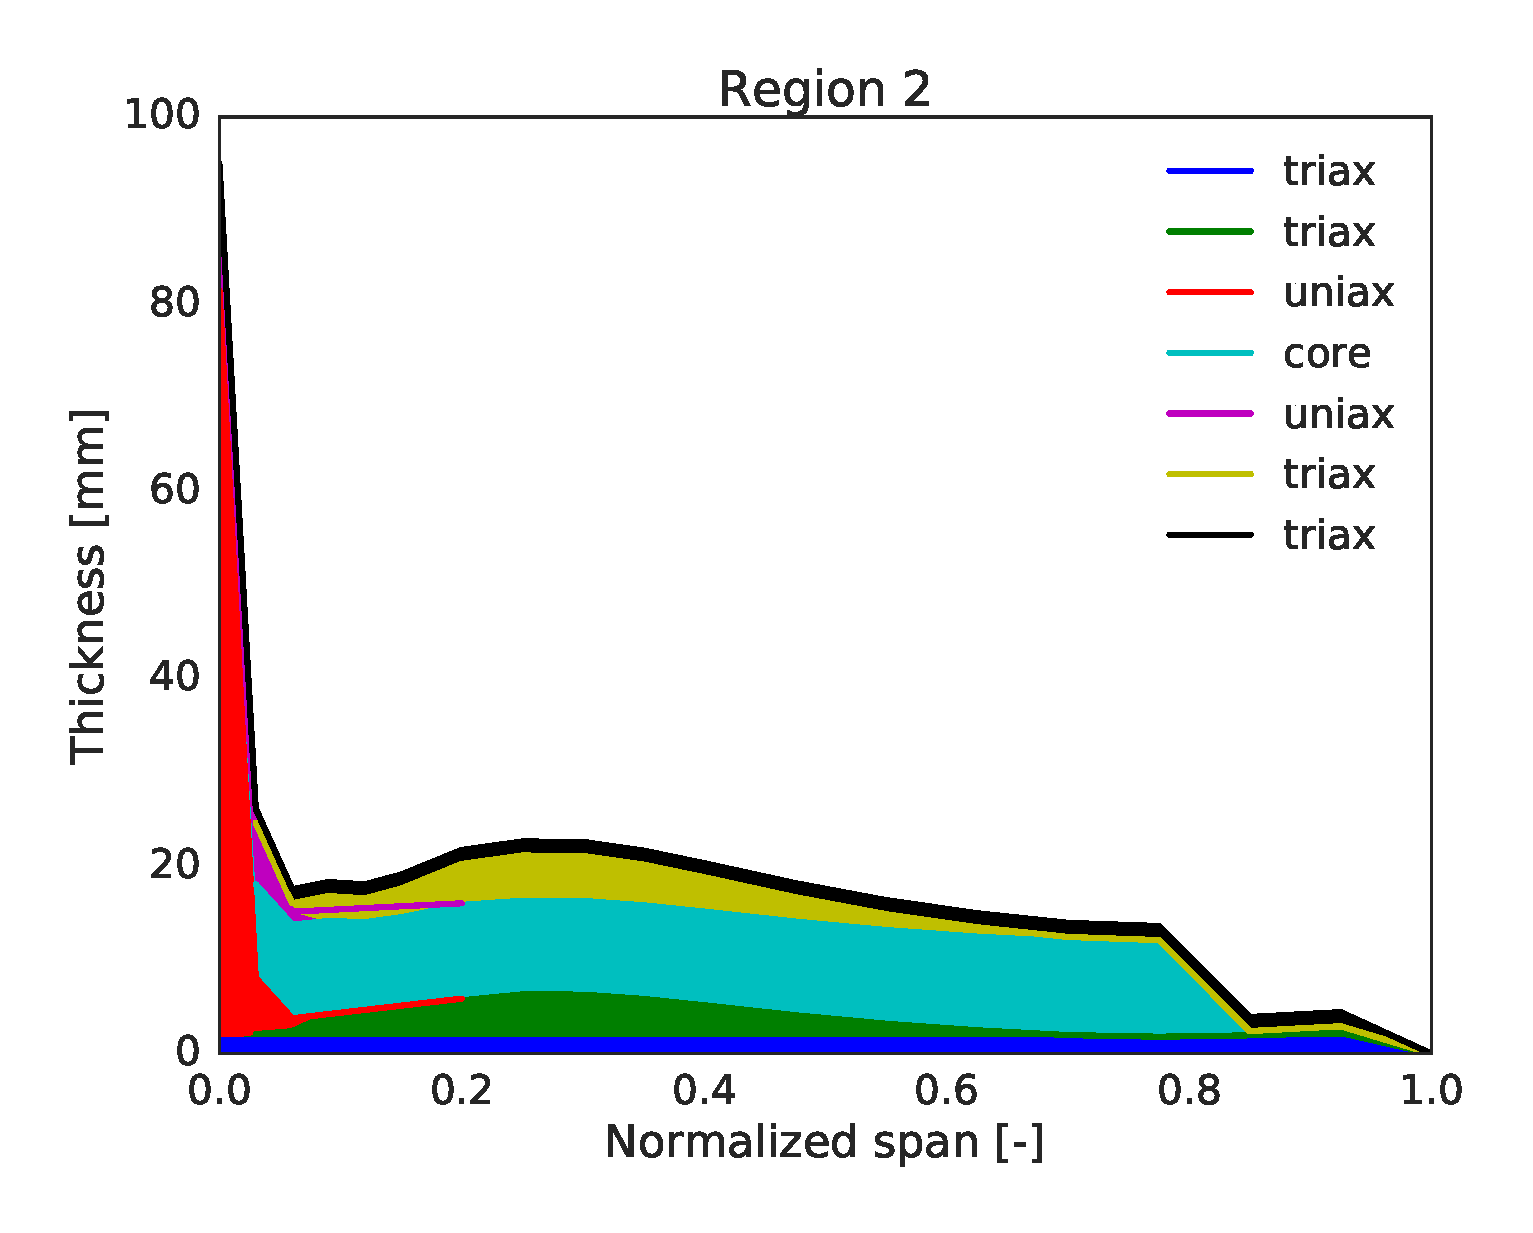
\includegraphics[width=\linewidth]{figures/KB6_final/KB6_laminate_layers_r02.eps}
\caption{Laminate layup of KB6 blade}
\label{subfig:KB6_layers_r02}
\end{subfigure}

\begin{subfigure}{\textwidth}
\centering
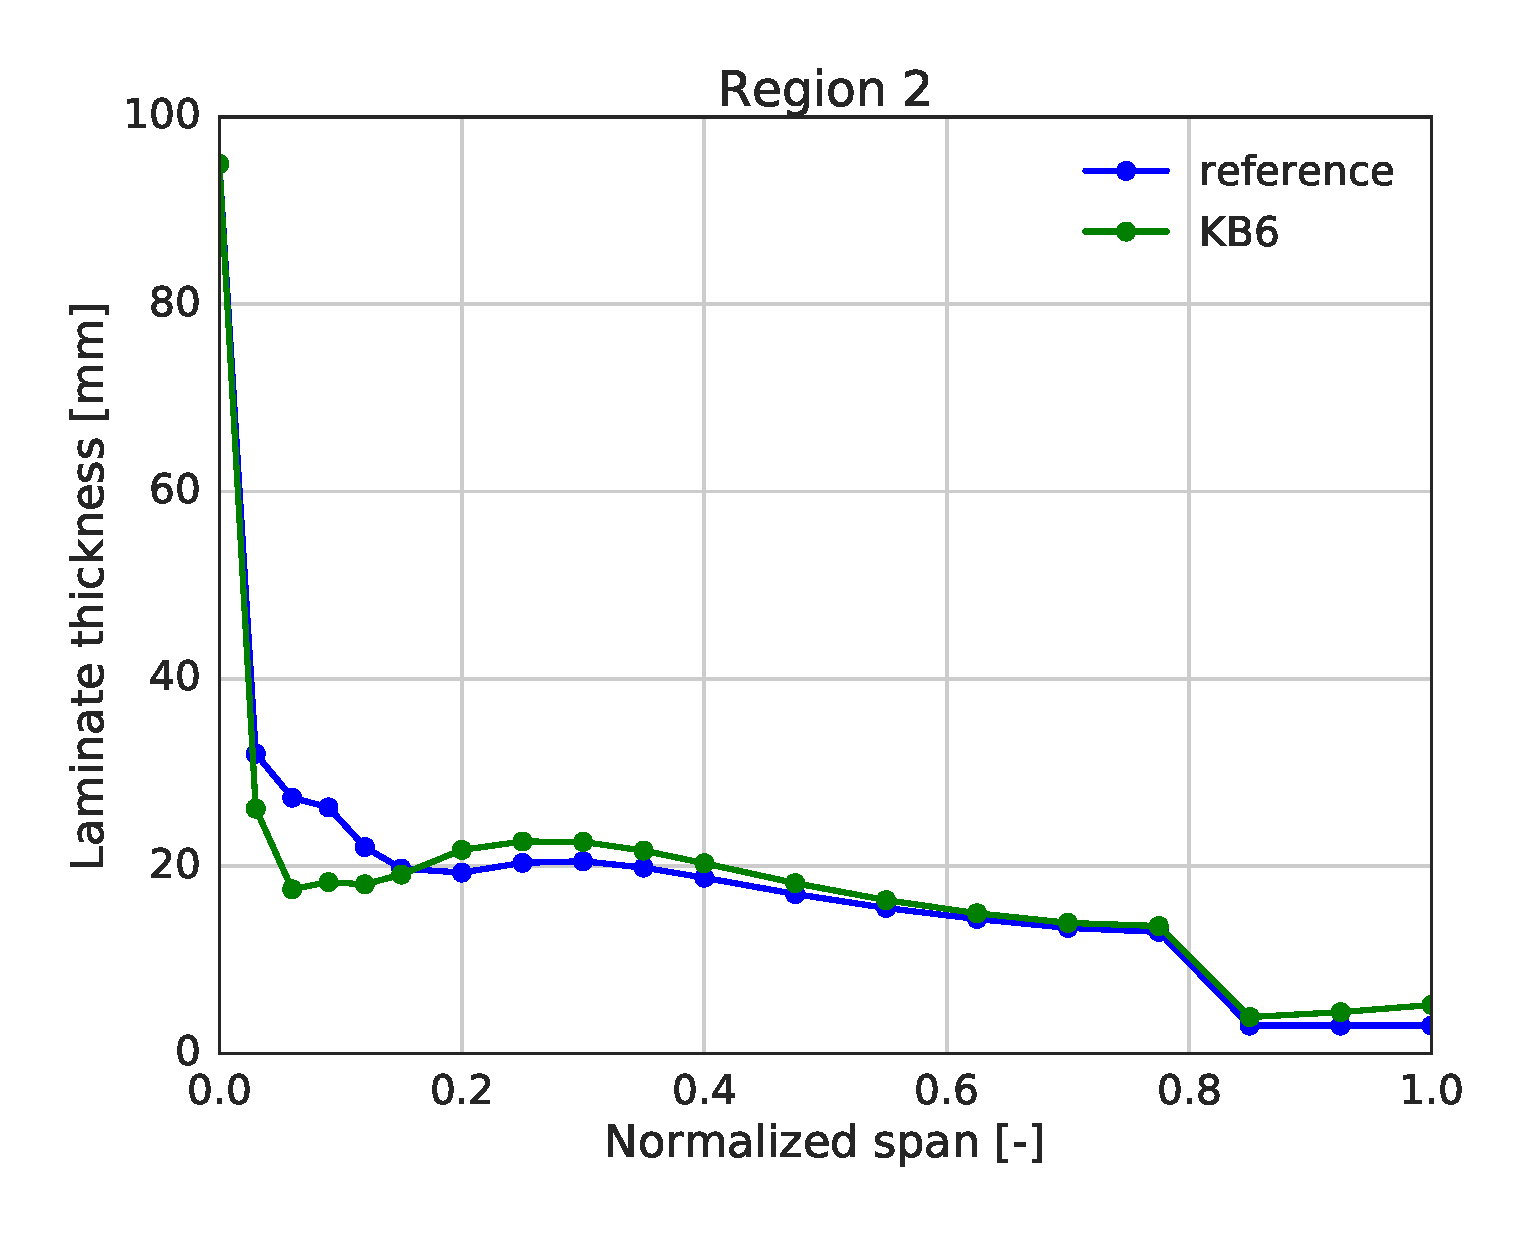
\includegraphics[width=0.50\linewidth]{figures/KB6_final/KB6_r02_thickness.eps}
\caption{Laminate thickness comparison of KB6 with reference}
\label{subfig:KB6_thick_r02}
\end{subfigure}
\caption{ Material in the main panel (immediately behind the spar cap)}
\label{fig:KB6_mat_r02}
\end{figure}

%region 4
\begin{figure}[tph]
\begin{subfigure}{0.50\textwidth}
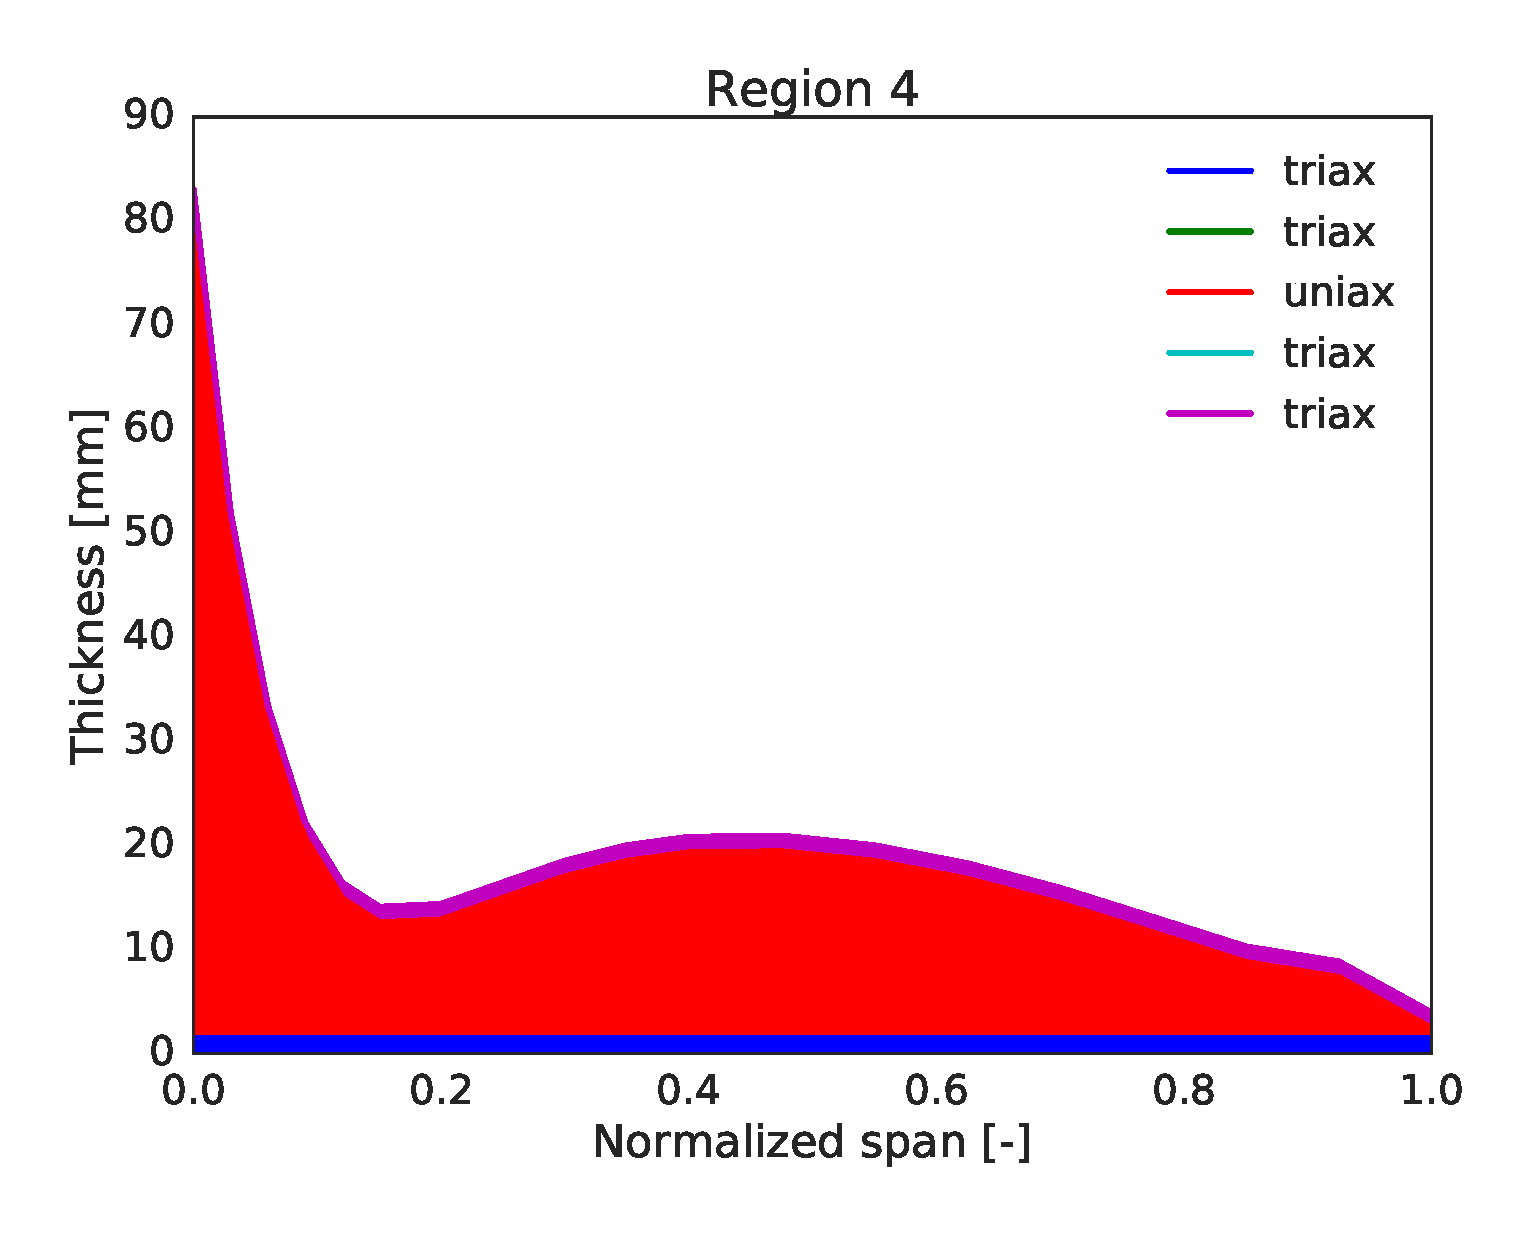
\includegraphics[width=\linewidth]{figures/KB6_final/baseline_laminate_layers_r04.eps}
\caption{Laminate layup of reference blade}
\label{subfig:baseline_layers_r04}
\end{subfigure}
 ~
\begin{subfigure}{0.50\textwidth}
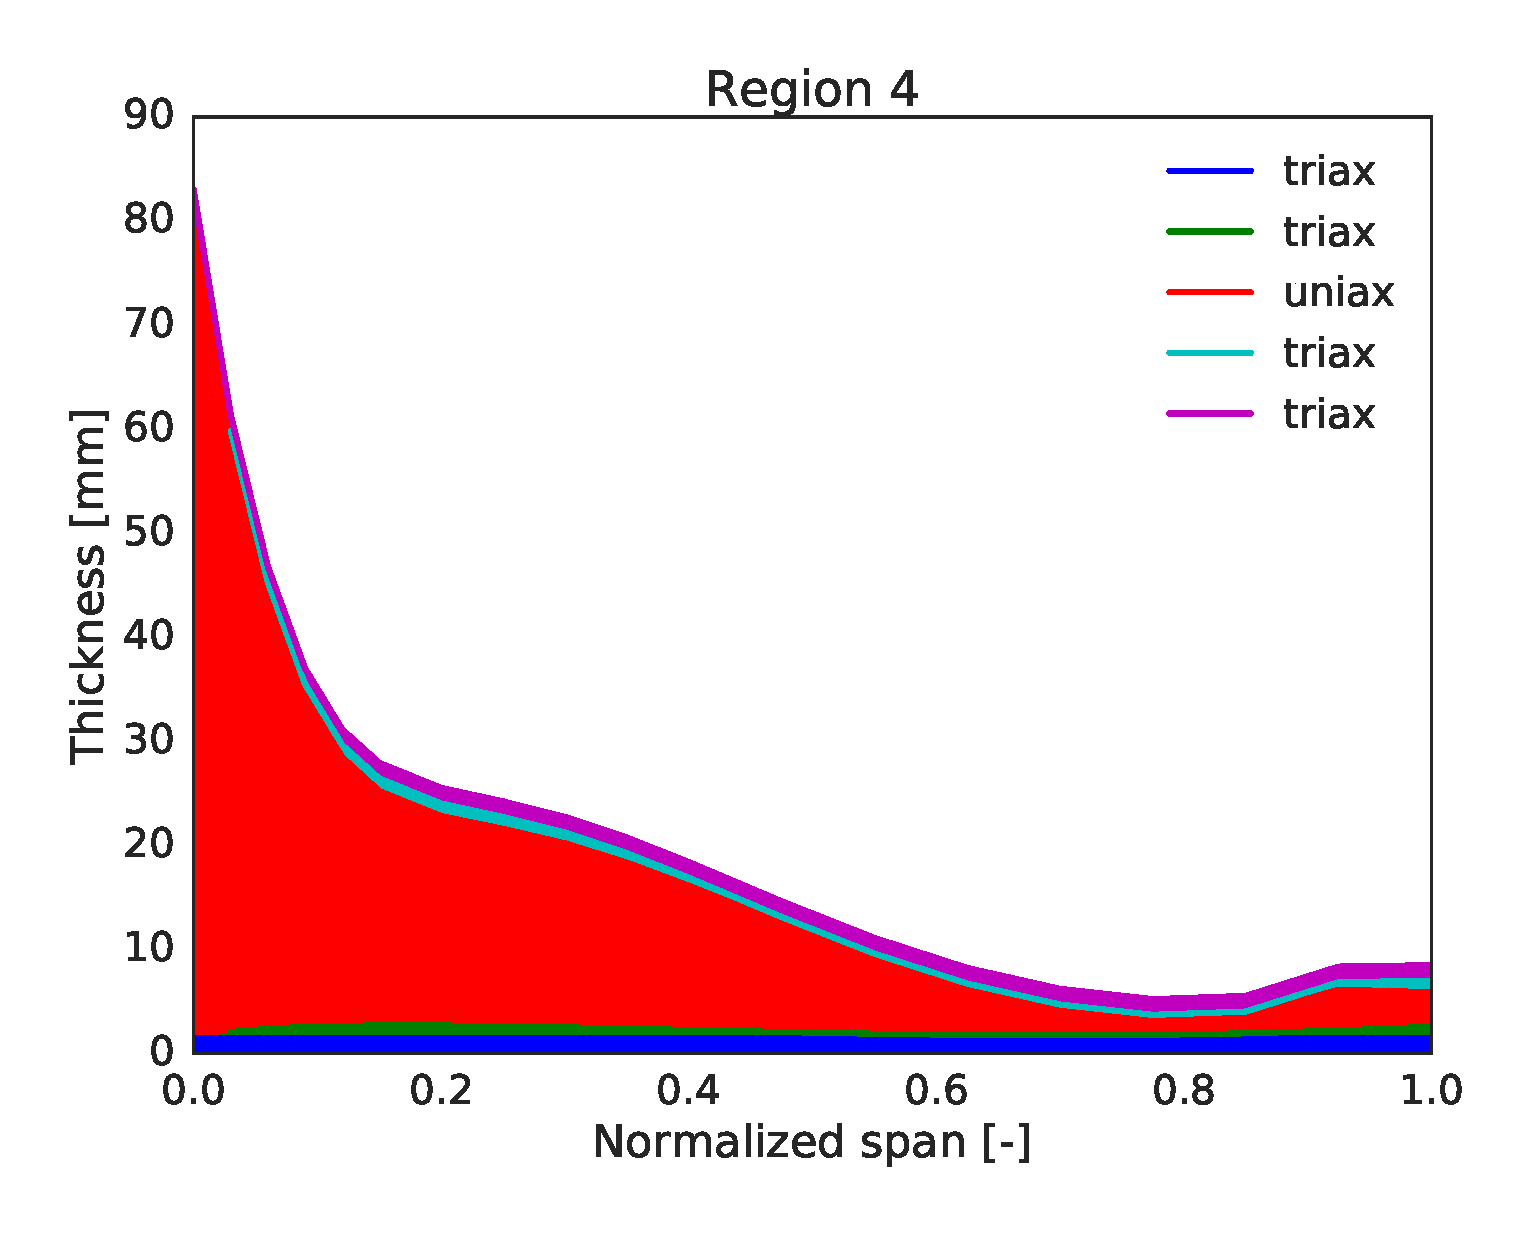
\includegraphics[width=\linewidth]{figures/KB6_final/KB6_laminate_layers_r04.eps}
\caption{Laminate layup of KB6 blade}
\label{subfig:KB6_layers_r04}
\end{subfigure}

\begin{subfigure}{\textwidth}
\centering
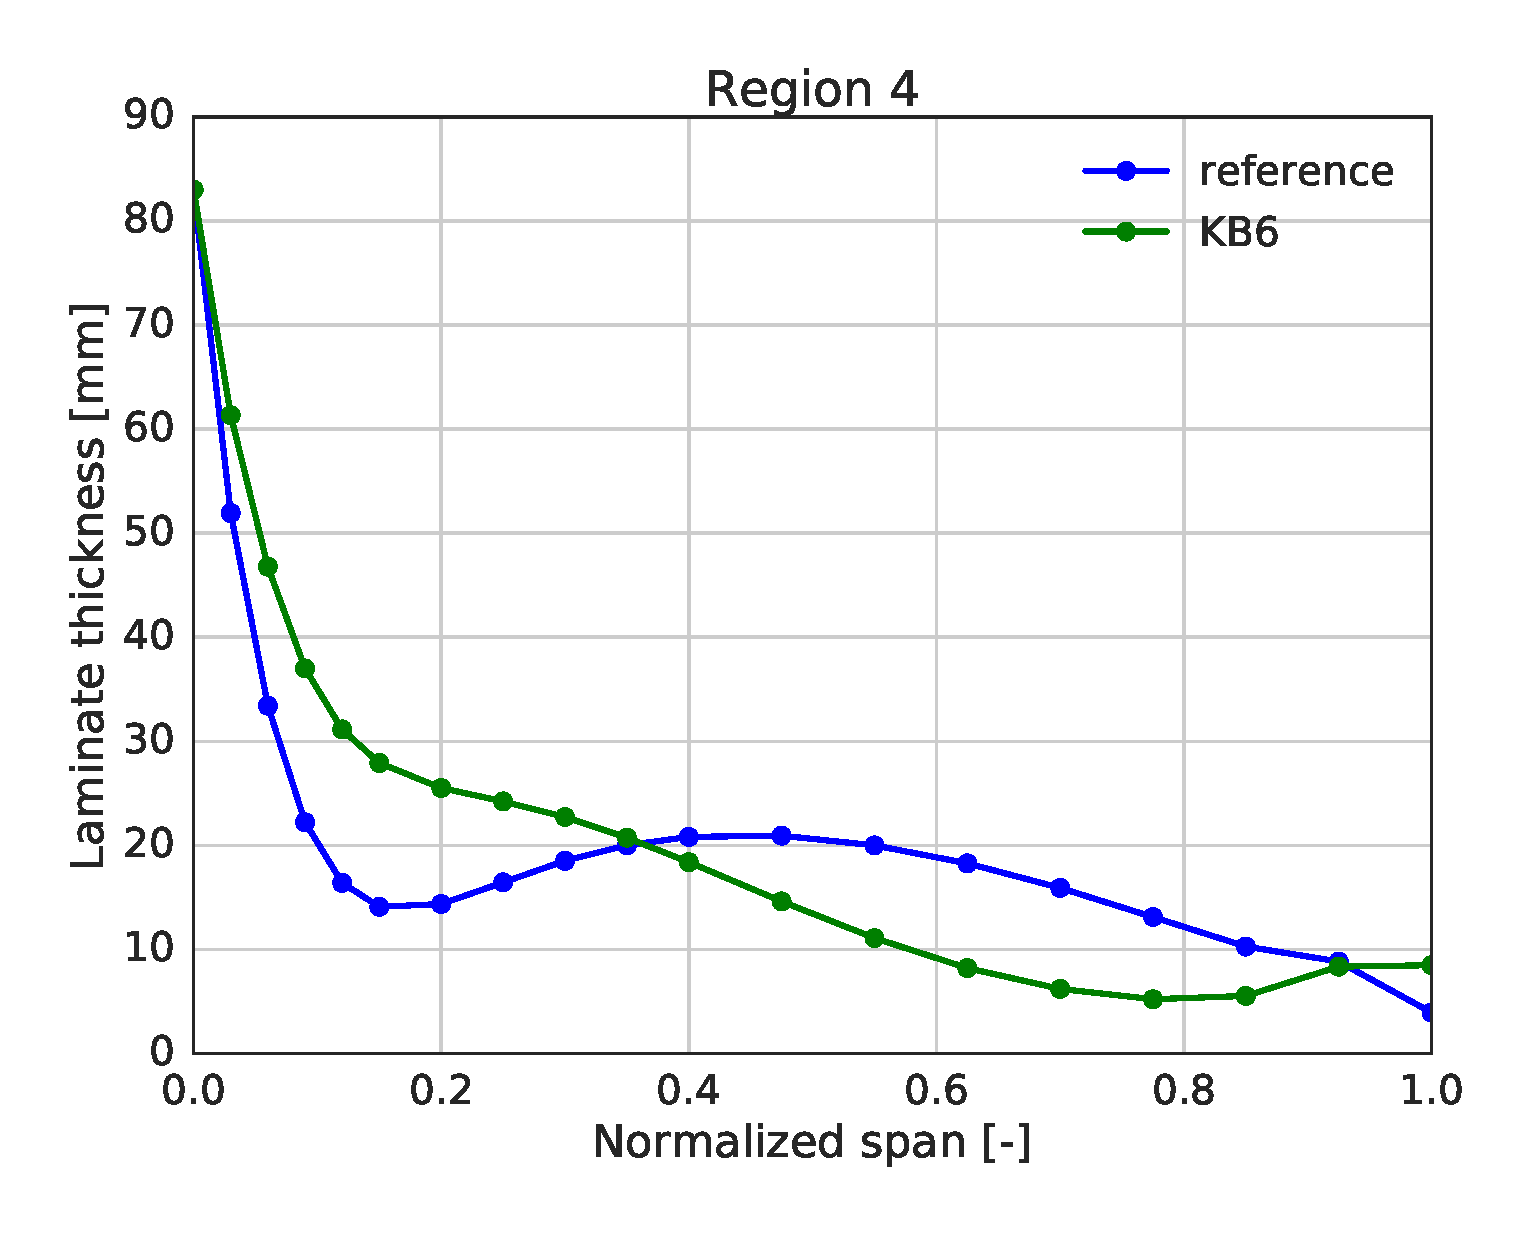
\includegraphics[width=0.50\linewidth]{figures/KB6_final/KB6_r04_thickness.eps}
\caption{Laminate thickness comparison with reference}
\label{subfig:KB6_thick_r04}
\end{subfigure}
\caption{ Material in the spar cap}
\label{fig:KB6_mat_r04}
\end{figure}

%region 6
\begin{figure}[tph]
\begin{subfigure}{0.50\textwidth}
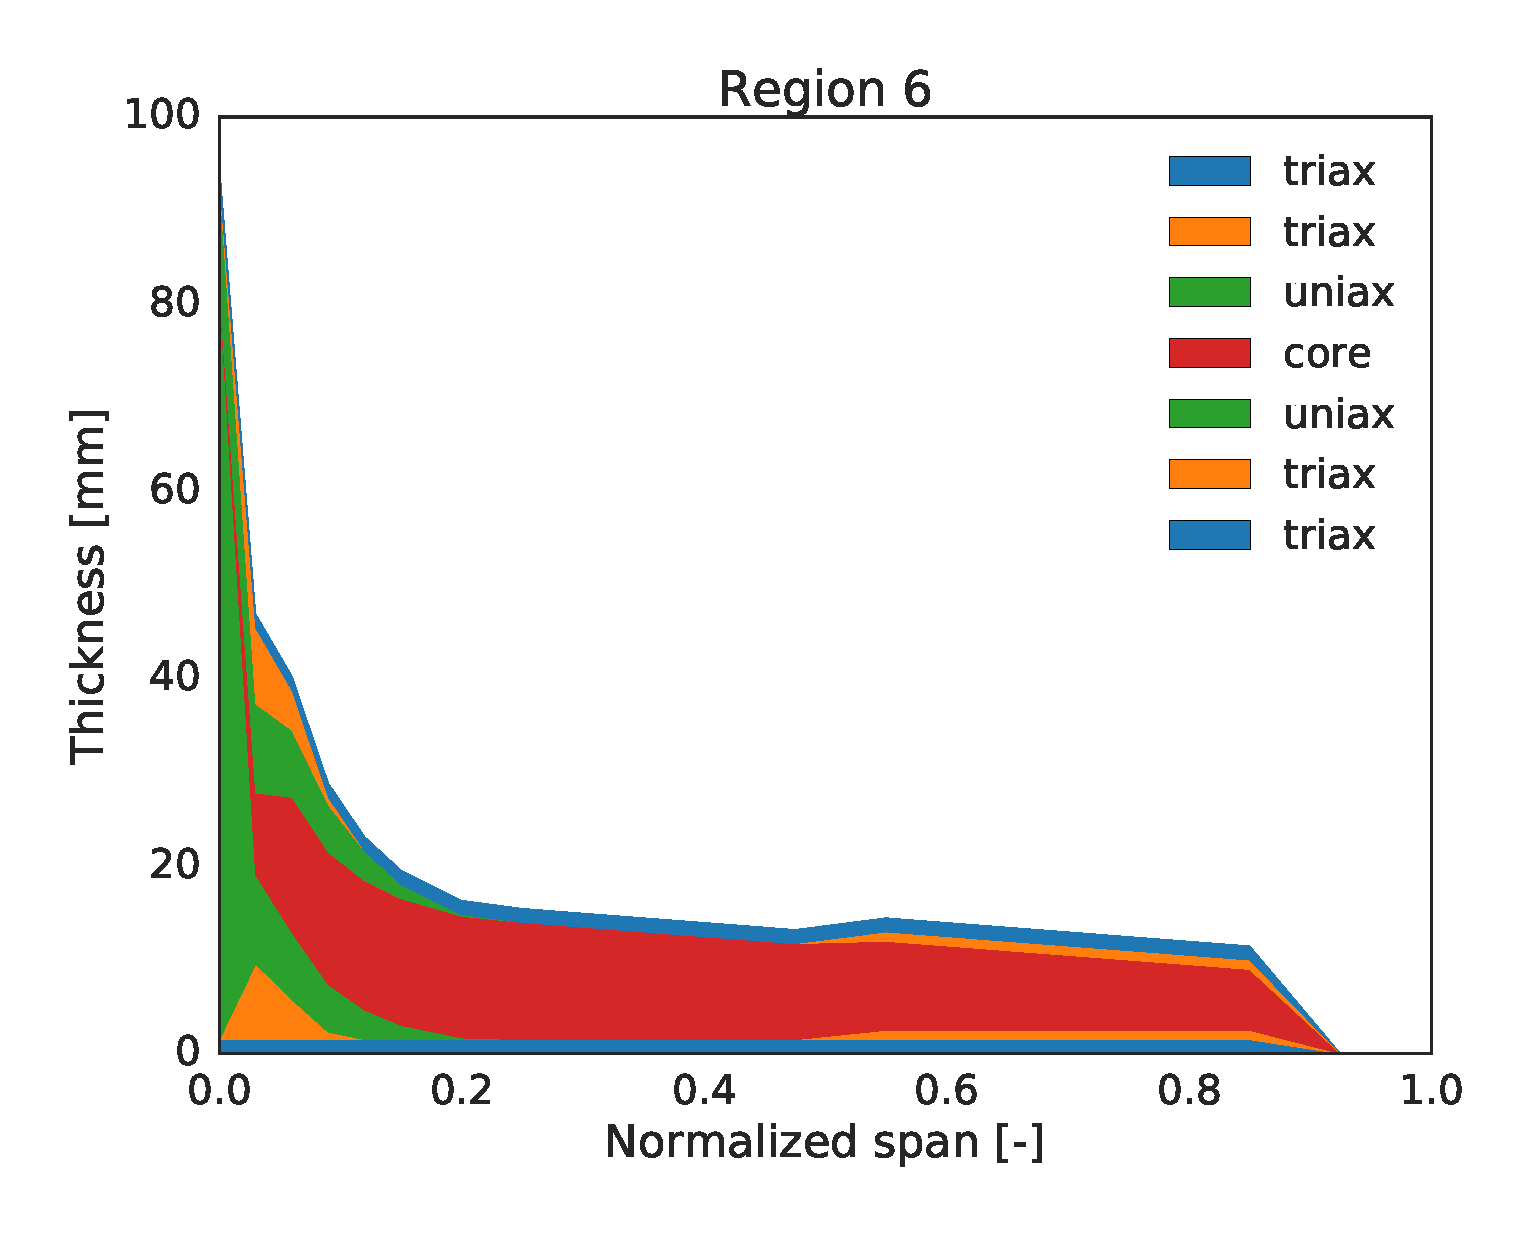
\includegraphics[width=\linewidth]{figures/KB6_final/baseline_laminate_layers_r06.eps}
\caption{Laminate layup of reference blade}
\label{subfig:baseline_layers_r06}
\end{subfigure}
 ~
\begin{subfigure}{0.50\textwidth}
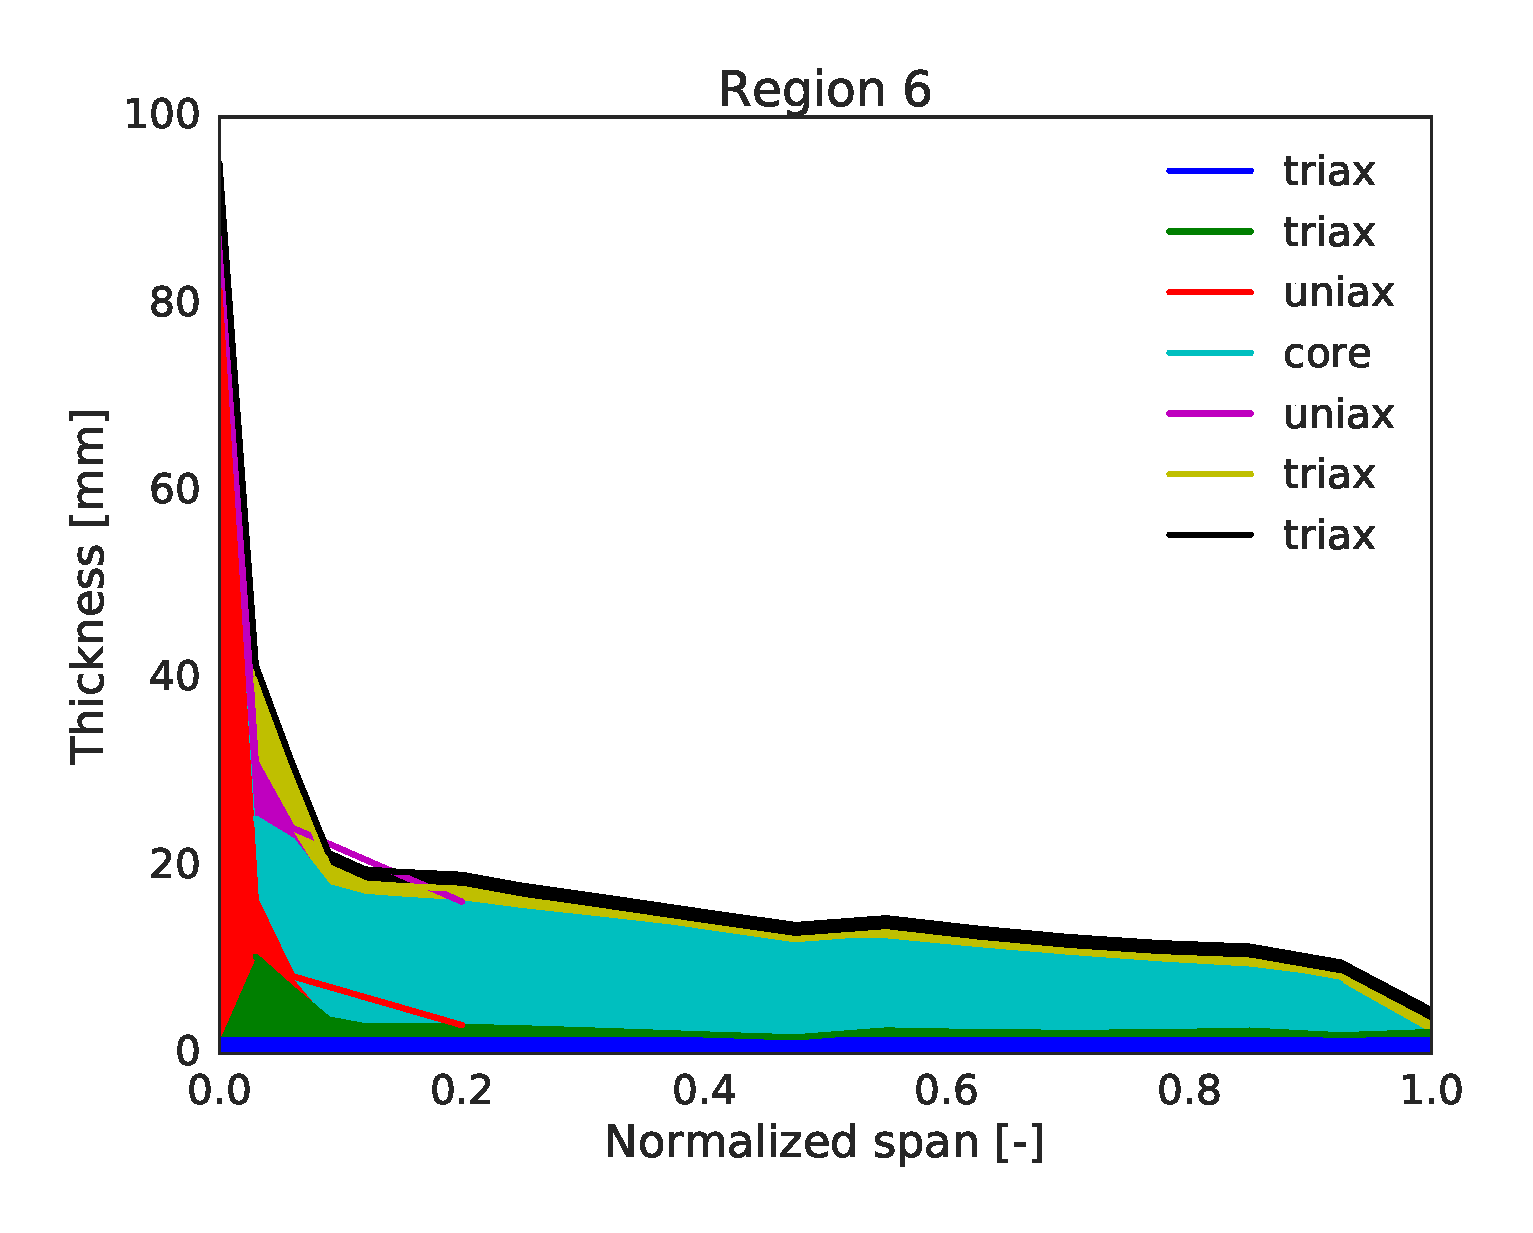
\includegraphics[width=\linewidth]{figures/KB6_final/KB6_laminate_layers_r06.eps}
\caption{Laminate layup of KB6 blade}
\label{subfig:KB6_layers_r06}
\end{subfigure}

\begin{subfigure}{\textwidth}
\centering
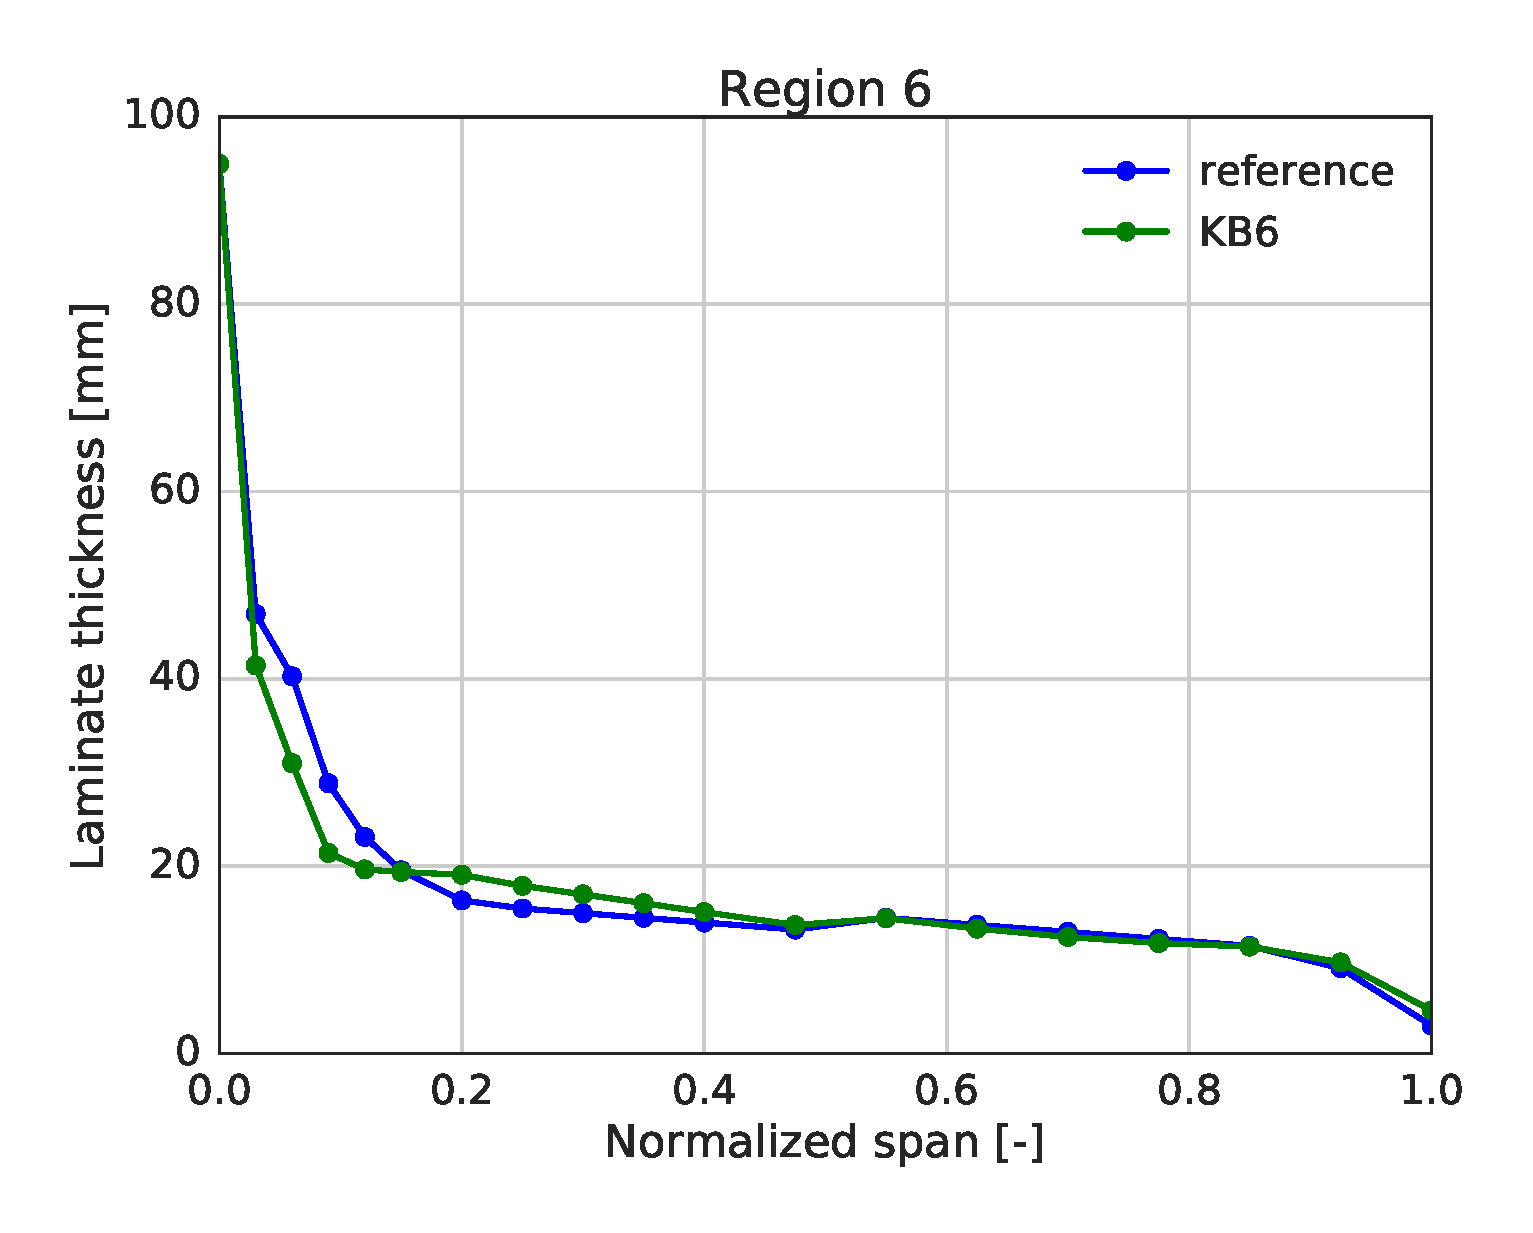
\includegraphics[width=0.50\linewidth]{figures/KB6_final/KB6_r06_thickness.eps}
\caption{Laminate thickness comparison of KB6 with reference}
\label{subfig:KB6_thick_r06}
\end{subfigure}
\caption{ Material in the leading region (immediately in front of the spar cap)}
\label{fig:KB6_mat_r06}
\end{figure}

%region 7
\begin{figure}[tph]
\begin{subfigure}{0.50\textwidth}
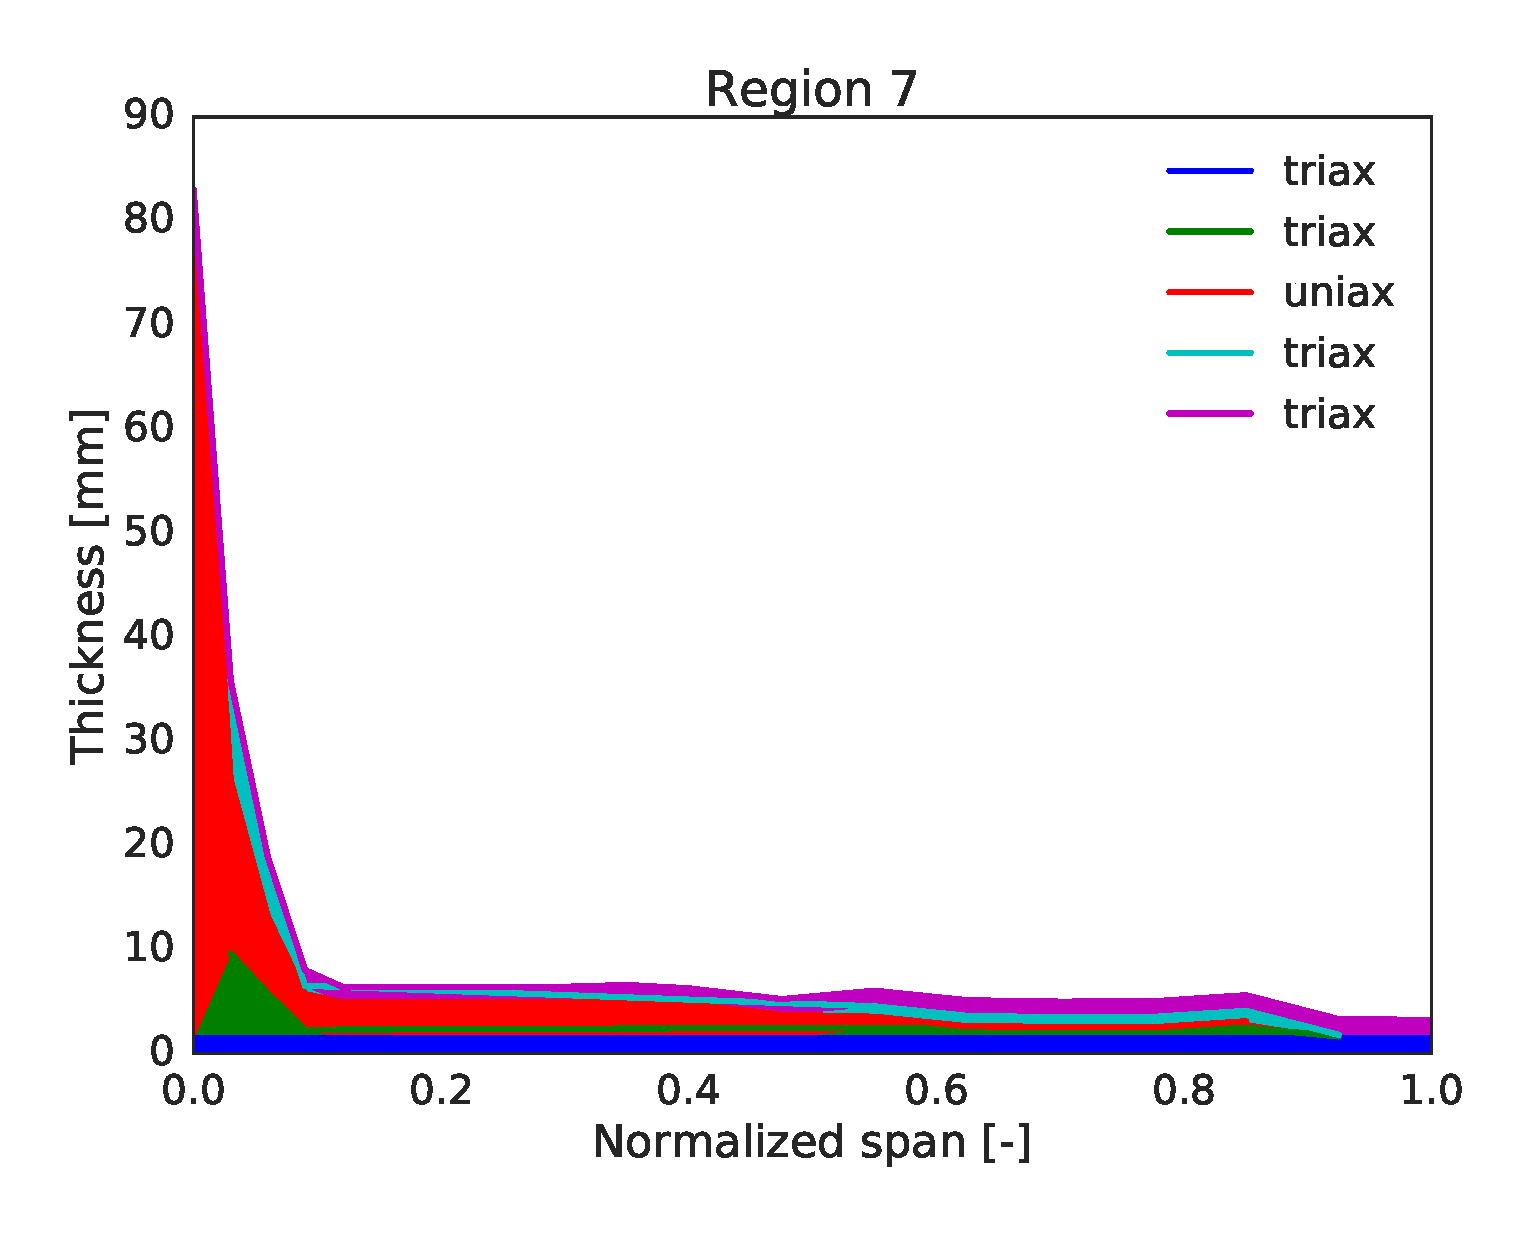
\includegraphics[width=\linewidth]{figures/KB6_final/baseline_laminate_layers_r07.eps}
\caption{Laminate layup of reference blade}
\label{subfig:baseline_layers_r07}
\end{subfigure}
 ~
\begin{subfigure}{0.50\textwidth}
\includegraphics[width=\linewidth]{figures/KB6_final/KB6_laminate_layers_r07.eps}
\caption{Laminate layup of KB6 blade}
\label{subfig:KB6_layers_r07}
\end{subfigure}

\begin{subfigure}{\textwidth}
\centering
\includegraphics[width=0.50\linewidth]{figures/KB6_final/KB6_r07_thickness.eps}
\caption{Laminate thickness comparison with reference}
\label{subfig:KB6_thick_r07}
\end{subfigure}
\caption{ Material in the leading edge reinforcement}
\label{fig:KB6_mat_r07}
\end{figure}

%% stiffnesses
%
\begin{figure}[tph]
\begin{subfigure}{0.50\textwidth}
\includegraphics[width=\linewidth]{figures/KB6_final/KB6_flapStiff_log.eps}
\caption{Flapwise stiffness on log scale}
\label{subfig:KB6_flapstiff_log}
\end{subfigure}
 ~
\begin{subfigure}{0.50\textwidth}
\includegraphics[width=\linewidth]{figures/KB6_final/KB6_flapStiff_ratio.eps}
\caption{Flapwise stiffness ratio (KB6/reference)}
\label{subfig:KB6_flapstiff_ratio}
\end{subfigure}

\begin{subfigure}{0.50\textwidth}
\includegraphics[width=\linewidth]{figures/KB6_final/KB6_edgeStiff_log.eps}
\caption{Edgewise stiffness on log scale}
\label{subfig:KB6_edgestiff_log}
\end{subfigure}
 ~
\begin{subfigure}{0.50\textwidth}
\includegraphics[width=\linewidth]{figures/KB6_final/KB6_edgeStiff_ratio.eps}
\caption{Edgewise stiffness ratio (KB6/reference)}
\label{subfig:KB6_edgestiff_ratio}
\end{subfigure}

\begin{subfigure}{0.50\textwidth}
\includegraphics[width=\linewidth]{figures/KB6_final/KB6_torsStiff_log.eps}
\caption{Torsional stiffness on log scale}
\label{subfig:KB6_torsstiff_log}
\end{subfigure}
 ~
\begin{subfigure}{0.50\textwidth}
\includegraphics[width=\linewidth]{figures/KB6_final/KB6_torsStiff_ratio.eps}
\caption{Torsional stiffness ratio (KB6/reference)}
\label{subfig:KB6_torsstiff_ratio}
\end{subfigure}

\caption{ Stiffness comparisons with reference.}
\label{fig:KB6_stiffness}
\end{figure}

\subsection{Steady-state performance}
The steady state operational performance and load response are discussed. It is important to note that the results being discussed in this section pertain to the response of the blade design as recorded during the optimization. The calculations during the optimization are performed in the aeroelastic code HAWCStab2, wherein a nonlinear finite element beam model is coupled with an unsteady blade element momentum (BEM) aerodynamic model considering induction from the shed vorticity, dynamic stall and dynamic inflow \cite{hawcstab2}.

The steady state power and thrust of the KB6 rotor is shown in Figure \ref{fig:KB6_power_thrust}. The KB6 rotor generates rated power at a wind speed of 10 m/s whereas the reference rotor produces the same at 11 m/s, as seen in Figure \ref{subfig:KB6_pcurve}. The power produced by KB6 is higher in the variable speed region with the greatest difference of 11.4 kW observed at a wind speed of 9.5 m/s. From Figure \ref{subfig:KB6_thrust} presenting the thrust curve, it is seen that the thrust too is greater in KB6 in the variable speed region. However, the peak thrust produced at a wind speed of 9.5m/s is 0.5\% lower than the reference turbine. The optimal power coefficient for the KB6 rotor is $0.476$ and is held constant in the variable speed region until the wind speed between 8 and 9 m/s where the rated rotor speed of $70$ rpm is attained. This is shown in Figure \ref{subfig:KB6_CP}. Beyond this point and until it attains the rated power at a wind speed of 10 m/s, the power coefficient decreases as a result of decreasing tip-speed ratio with rising wind speed. Whereas the reference rotor has a optimal constant power coefficient of $0.46$ which is maintained until it attains the rated rotor speed of $70$ rpm at a wind speed of 10 m/s. Figure \ref{subfig:KB6_CT} shows the thrust coefficient over the operational wind speed range of the turbine. The thrust coefficient for KB6 is higher than that for the reference rotor, and it decreases with rising wind speed in the variable speed region. This is a result of the blade increasingly twisting towards the feather with rising wind speed due to the bend-twist coupling effect as a consequence of the backward sweep in the blade. Due the backward sweep, a larger flapwise force will generate greater torsional moments resulting in increased torsion towards feather. The decrease in the thrust coefficient is even greater beyond the 8 - 9 m/s wind speed range, during which the KB6 rotor attains rated rotor speed. This decrease is due to the reduction in loading as a result of decreasing tip-speed ratio additionally contributing to the load reduction being offered by the geometric bend-twist coupling. Such passive load alleviation mechanisms allow for a larger rotor that can produce more power for a considerably low increase of the aerodynamic loads over those produced by the reference rotor. Furthermore, the peak loading is similar to that of the reference rotor.  

The steady state load response of the KB6 and reference rotors are shown in Figure \ref{fig:KB6_load_response}. The flapwise blade root bending moment is increased in KB6 compared to the reference rotor, primarily due the 5.5\% increase in the blade length. This can be observed in Figure \ref{subfig:KB6_Mx}. The edgewise blade root bending moment is shown in Figure \ref{subfig:KB6_My}. It is seen to be slightly lower than the reference rotor. Edgewise moments are mainly driven by the mass of the blade and the reductions can be attributed to the 4.65\% lower blade mass of the KB6 rotor than the reference. The torsional moments shown in Figure \ref{subfig:KB6_Mz}, are seen to increase in absolute magnitude, with rising wind speeds in the variable speed region of the KB6 rotor. This is due the backward sweep of the blade that generates additional torsional moment due to the action of the flapwise forces, which increase with rising wind speeds. The negative sign of the torsional moments indicate that the moments are directed in twisting the blade towards the feather. Thus, for rising wind speeds, the increasing flapwise force makes the blade twist increasingly towards the feather. Beyond the point at which the rated rotor speed is attained for the KB6 rotor, the decreasing tip-speed ratio slightly reduces the flapwise forces thus relatively reducing the magnitude of the torsional moment until 10 m/s at which rated power is achieved. Beyond this point the same phenomenon is repeated, but is mainly driven by reduction in the tip-speed ratio caused by pitching of the blades.

The steady state physical response of the structure is shown in Figure \ref{fig:KB6_deflections}. Figure \ref{subfig:KB6_tors_posn} shows the steady state torsional response of the rotor at a wind speed of 9 m/s. The KB6 blade is seen to torsion towards the feather with the absolute magnitude increasing with the normalized span. The increase in torsion corresponds to the increase in the amount of backward sweep along the span, as seen in Figure \ref{subfig:KB6_sweep}. The spanwise blade torsion with increasing wind speeds in the variable speed region is shown in Figure \ref{subfig:KB6_tors_posn_diffwsp}. It is seen that the blade twists increasingly towards the feather for increasing wind speeds, until 85\% blade span. For the last 15\% of the KB6 blade span the blade twists increasingly towards stall with rising wind speeds. %%%SHould I write about the prebend affecting the torsion as it reduces the flapwise force distribution?? But maybe a further analysis is required to support it.
The flapwise positions of the blade sections are shown in Figure \ref{subfig:KB6_flap_posn} at a wind speed of 9 m/s. The KB6 blade is seen to bend towards the tower with its magnitude increasing along the span until approximately 80\% of the blade length. At this point the blade attains a position closest to the tower. Beyond this point the blade is seen to deflect away from the tower relative to its closest position, until the tip. %\textcolor{red}{This behaviour is attributed to the large gradient in the prebend for the corresponding spanwise location. }
Figure \ref{subfig:KB6_flap_pson_diffwsp} shows the flapwise positions of the blade for different wind speeds in the variable speed region of the KB6 rotor. The blade increasingly deflects towards the tower with rising wind speeds, due to increasing flapwise bending moments as seen in Figure \ref{subfig:KB6_Mx}. The flapwise bending moment moment is seen to attain its highest value at a wind speed of 9 m/s corresponding to the resulting flapwise blade positions.

The angles of attack along the span for different wind speeds in the variable speed region of the KB6 rotor is seen in Figure \ref{fig:KB6_aoa}. The angles of attack are seen to decrease with rising wind speeds until the wind speed of 8 m/s. The KB6 rotor attains its rotor speed between a wind speed of 8 m/s and 9 m/s, marking the end of the variable speed region. At a wind speed of 9m/s the angles of attack are seen to attain a higher value than the rest of the wind speeds. %%Is the airfoil entering stall? Need Cl to examine that. What is the design angle of attack of the new airfoils? Need Cl/Cd to get region of maximum efficiency.....
% power and thrust 
\begin{figure}[tph]
\begin{subfigure}{0.50\textwidth}
\includegraphics[width=\linewidth]{figures/KB6_final/KB6_power_diff_HS2.eps}
\caption{Power curve with absolute difference from reference}
\label{subfig:KB6_pcurve}
\end{subfigure}
 ~
\begin{subfigure}{0.50\textwidth}
\includegraphics[width=\linewidth]{figures/KB6_final/KB6_thrust_HS2.eps}
\caption{Thrust curve}
\label{subfig:KB6_thrust}
\end{subfigure}

\begin{subfigure}{0.50\textwidth}
\includegraphics[width=\linewidth]{figures/KB6_final/KB6_Cp_HS2.eps}
\caption{Power coefficient curve}
\label{subfig:KB6_CP}
\end{subfigure}
 ~
\begin{subfigure}{0.50\textwidth}
\includegraphics[width=\linewidth]{figures/KB6_final/KB6_CT_HS2.eps}
\caption{Thrust coefficient curve}
\label{subfig:KB6_CT}
\end{subfigure}

\caption{Steady state power and thrust curves}
\label{fig:KB6_power_thrust}
\end{figure}

% load response
\begin{figure}[tph]
\begin{subfigure}{0.50\textwidth}
\includegraphics[width=\linewidth]{figures/KB6_final/KB6_MxBR_HS2.eps}
\caption{Flapwise blade root bending moment}
\label{subfig:KB6_Mx}
\end{subfigure}
 ~
\begin{subfigure}{0.50\textwidth}
\includegraphics[width=\linewidth]{figures/KB6_final/KB6_MyBR_HS2.eps}
\caption{Edgewise blade root bending moment}
\label{subfig:KB6_My}
\end{subfigure}

\begin{subfigure}{\textwidth}
\centering
\includegraphics[width=0.50\linewidth]{figures/KB6_final/KB6_steady_MzBR_HS2.eps}
\caption{Torsional blade root moment}
\label{subfig:KB6_Mz}
\end{subfigure}
 
\caption{Steady state load response}
\label{fig:KB6_load_response}
\end{figure}

%% torsion, blade tip deflection
\begin{figure}[tph]
\begin{subfigure}{0.50\textwidth}
\includegraphics[width=\linewidth]{figures/KB6_final/KB6_torsion_09.eps}
\caption{Torsion at 9m/s}
\label{subfig:KB6_tors_posn}
\end{subfigure}
 ~
\begin{subfigure}{0.50\textwidth}
\includegraphics[width=\linewidth]{figures/KB6_final/KB6_torsion_diffwsp.eps}
\caption{Torsion for different wind speeds in the variable speed region}
\label{subfig:KB6_tors_posn_diffwsp}
\end{subfigure}

\begin{subfigure}{0.50\textwidth}
\includegraphics[width=\linewidth]{figures/KB6_final/KB6_Flap_deflec_HS2.eps}
\caption{Flapwise blade tip position}
\label{subfig:KB6_flap_posn}
\end{subfigure}
 ~
\begin{subfigure}{0.50\textwidth}
\includegraphics[width=\linewidth]{figures/KB6_final/KB6_Flap_deflec_WSP_HS2.eps}
\caption{Flapwise blade tip position for wind speeds in variable speed region}
\label{subfig:KB6_flap_pson_diffwsp}
\end{subfigure}

\caption{Steady state blade response}
\label{fig:KB6_deflections}
\end{figure}

%%Angle of attack

\begin{figure}[tph]
\centering
\includegraphics[width=0.8\linewidth]{figures/KB6_final/KB6_AoA_WSP_HS2.eps}
\caption{Steady state angles of attack along the blade span for wind speeds in variable speed region}
\label{fig:KB6_aoa}
\end{figure}

\section{Conclusion}
\label{sec:optimize_conc}
The reference 100 kW rotor has been optimized using the multi-disciplinary optimization tool HawtOpt2. Five different optimized blades were obtained through placing varying constraints in the problem formulation. KB1 was optimized as a straight blade with no coupling. KB2 was optimized as a geometrically coupled blade through the introduction of backward sweep. KB3 was optimized as a material coupled blade through altering the fibre layup angles in the spar cap uniax laminates. Based on an analysis of the obtained optimized designs it was decided to select backward sweep as the means to introduce bend-twist coupling. This was influenced by the superior power output and annual energy production of the KB2 swept design over the KB3 material coupled design. Additional constraints on the maximum achievable backward sweep and prebend were placed on the design to facilitate manufacturability.  

The optimized designs showed significant improvements in the annual energy production over the reference turbine. The coupled designs provided a greater improvement than the non-coupled design due to the passive load reduction afforded by bend-twist coupling. This allowed for the optimized blades to be more slender, flexible, longer and at the same time have a lower mass than the reference blade. The optimized rotor further curtailed peak loads by attaining the rated rotor speed at an earlier wind speed than the rated power. Providing design freedom to the tip-speed ratio and in extension to the rotor speed also aided in improving the annual energy production.

\clearpage
\chapter{Static load test}
\label{ch:load_test}

\section{Introduction}
\label{sec:static_intro}
The structural response of the finalized blade design KB6 under the action of a static flapwise force at the blade tip is presented. The response is compared with the reference blade.  
\clearpage
\chapter{Analysis of the Design Load Basis}

\section{Introduction}

The design load basis considered for this report is based on the IEC 61400-1 standard. A more elaborate discussion and interpration of that standard is given in \cite{hansen_design_2015}.

The following rotor configurations have been considered:
\begin{itemize}
	\item reference (referred to as baseline or baseline100kw in the figures)
	\item KB1
	\item KB2
\end{itemize}

The figures included in the appendices \ref{app:baseline-vs-KB1} and \ref{app:baseline-vs-KB2} show the minima, mean, maxima and standard deviations for all of the simulations considered within the given design load case. For a more elaborate description of those cases the reader is referred to \cite{hansen_design_2015}.

This report does not include selected time series plots of the design load basis analysis, although some of the conclusions presented within the the discussion section (see section \ref{sec:dlb:discussion}) are based on the analysis of individual time series.

Appendix \ref{app:baseline-vs-KB1} and \ref{app:baseline-vs-KB2} include the comparison between the reference rotor and KB1, and reference rotor and KB2 respectively. The following channels are considered:
\begin{itemize}
	\item Electrical power [W], excluding losses.
    \item Rotor speed [rpm]
    \item Blade 1, 2 and 3 pitch angles [deg]
    \item Controller status flag [0-6], 0: normal operation, 1: shut down due to over speed
    \item Tower base for-aft bending moment [kNm]
    \item Tower base side-side bending moment [kNm]
    \item Yawing moment tower top [kNm]
    \item Shaft torsion moment [kNm]
    \item Blade root 1, 2 and 3 flap-wise bending moments [kNm] (pitching coordinates)
    \item Blade root 1, 2 and 3 edge-wise bending moments [kNm] (pitching coordinates)
    \item Blade root 1, 2 and 3 torsion bending moments [kNm] (pitching coordinates)
    \item Minimum tower to blade tip distance [m] (consider only the minima
\end{itemize}

To accommodate the comparison the figures include two different rotors, but the wind speed or wind direction is slightly off-set from the actual value. For example, for each wind speed of 10 m/s, case 1 is plotted at a  value slightly below 10 m/s, and case 2 at a value slightly above. Both cases have been run at the same wind speed of 10 m/s.


\section{Stiff Tower}
\label{sec:dlb:Stiff Tower}

The tower stiffness was first estimated based on a quantitative description and drawings provided by the turbine manufacturer. However, the stiffness and mass properties of the derived structural model ended up being very close to the 3P frequency at rated wind speed and above. This resulted in a sharp increase in tower side-side, blade-edge and shaft torsional loads. Knowing that this turbine is actually produced and being operated in the field, it is assumed that tower model initially derived from the given data was not sufficiently accurate. Until more detailed structural data becomes available, the tower is considered to be stiff. Once a sufficiently accurate description of the tower is known a flexible tower model can be introduced to re-assess the design load basis. Depending on the eigenfrequencies and damping of the tower, the introduction of tower flexibility is expected to affect the results.


\section{Controller Tuning}
\label{sec:dlb:Controller Tuning}

For this study the basic DTU Wind Energy controller is used \cite{hansen_basic_2013}. The controller is tuned based on the reference rotor using the pole placement technique as implemented for a 1 DOF model in HAWCStab2. The effective controller tuning parameters of the test turbine, however, are unknown at this stage in the project.

The controller tuning settings are assumed to be fixed for all three rotors. This is due to practical limitations with respect to the platform and the corresponding controller on which the blade will be tested in a later stage of the project. However, the design procedure did not include any additional constraints to mitigate the effects of a fixed controller tuning setup. Under normal circumstances, a re-designed rotor requires different controller tuning parameters compared to the reference case. As the results in this section indicate, not re-tuning the controller has negative consequences for the turbine and blade loads. Future design iterations could include the definition and inclusion of a constrained that mimics the effect a fixed controller tuning on the blade loads.

In addition to DLC1.1, one extra load case is considered under normal operating conditions with wind shear and tower shadow, but without any turbulence. Additionally, a 1 m/s wind step is added to the wind speed towards the end of the simulation. The purpose of this load case to evaluate the response of the controller under the given quasi-steady inflow conditions, and can help in qualifying the effect of the constant controller tuning parameters. This test case is labelled as "test\_steadysteps".


\section{Discussion}
\label{sec:dlb:discussion}

Both KB1 and KB2 show an increased loading envelope compared to the reference design. When considering DLC12 (see section \ref{sec:baseline-vs-KB1:dlc12} a clear increase in standard deviations and min/max loads is observed for high wind speeds. However, this load increase is likely to be caused by a poorly tuned controller (KB1 and KB2 are operating with the tuning parameters of the reference case). Figure \ref{fig:baseline-vs-KB1:dlc12:status} (the controller status flag) further shows that for high wind speeds certain cases have resulted in a shut down procedure due to a rotor over speed condition (over speed conditions are defined here as a 50\% increase over rated rotor speed, but the actual constrains of the test turbine are unknown).

Figure \ref{fig:baseline-vs-KB1:dlc12:blade-root-torsion} indicates that at high wind speed the blade torsional loads are increased dramatically. However, the time series indicate that these extremes are connected to the turbine entering the over speed shut down state, and which is accompanied by the blades pitching out to 90 degrees.

When considering DLC12 cases of wind speeds of 18 m/s and lower, a modest but consistent load decrease is observed for the various channels included here. This indicates that the KB1 and KB2 designs are both performing as intended, expect for the response at higher wind speeds due to inappropriate controller tuning settings. If these controller tuning effects can be mitigated, both KB1 and KB2 could be considered as improved versions (higher AEP, lower loads) with respect to the reference rotor.

The comparison between the three rotors indicate that the controller tuning has an important effect on the loads. Knowing the load sensitivities with respect to controller tuning parameters should be considered in order to mitigate the uncertainties regarding the actual controller setup of the test turbine.


\section{Future Work}
\label{sec:dlb:Future Work}

The first iteration of the full DLB has indicated some additional points of attention before a second iteration of the design and full DLB evaluation report are to be considered:

\begin{itemize}
	\item Include time series analysis of certain indicative results.
	\item Determine an accurate model for the tower (eigenfreqencies, structural damping).
	\item Include a constrained in future design and optimization runs to evaluate the controllability of the rotor given a fixed controller tuning configuration.
	\item Re-evaluate rotor over-speed shut-down criteria.
	\item Sensitivity study regarding controller tuning to account for the uncertainty caused by the unknown actual controller tuning parameters of the platform.
	\item Tabulated results showing the differences in load statistics.
	\item Tabulated extreme loads observed within each of the DLB's.
	\item Brake down of fatigue loads, and life time fatigue loads.
\end{itemize}

%\input{conclusions}
\clearpage


\bibliographystyle{abbrvnat}
\bibliography{references.bib}

\appendix
%\newpage
\chapter{Design Load Basis Statistic Tables}
\section{Reference vs KB5}
\label{tables:baseline-vs-KB6}

\captionof{table}{Blades 1,2,3 root torsion moment [kNm]}
\begin{tabular}{lllll}
\toprule
                     & \multicolumn{2}{l}{baseline} &         KB5 &\\
\midrule
                 DLC &  max of max &  min of min &  max of max &  min of min \\
 dlc12\_iec61400-1ed3 &    0.628669 &   -0.662794 &      1.6108 &     -0.6864 \\
 dlc24\_iec61400-1ed3 &    0.813648 &   -0.681443 &        1.45 &   -0.654118 \\
 dlc31\_iec61400-1ed3 &   0.0920486 &   -0.240909 &    0.191699 &  -0.0842973 \\
 dlc41\_iec61400-1ed3 &    0.472522 &   -0.571366 &    0.422211 &   -0.572294 \\
 dlc64\_iec61400-1ed3 &     1.30718 &   -0.959426 &     3.28982 &    -3.22197 \\
    No turbulence &     4.21674 &    -3.46674 &     5.46346 &    -4.25006 \\
\bottomrule
\end{tabular}


\captionof{table}{Blades 1,2,3 root flap bending moment [kNm]}
\begin{tabular}{lllll}
\toprule
                     & \multicolumn{2}{l}{baseline} &         KB5 &\\
\midrule
                 DLC &  max of max &  min of min &  max of max &  min of min \\
 dlc12\_iec61400-1ed3 &     56.0374 &    -65.6522 &     38.8565 &    -62.5098 \\
 dlc24\_iec61400-1ed3 &     64.9552 &    -62.0349 &     43.1082 &    -58.4736 \\
 dlc31\_iec61400-1ed3 &     2.36137 &    -25.7876 &   -0.388214 &    -25.4932 \\
 dlc41\_iec61400-1ed3 &     11.4245 &    -25.7876 &     8.20715 &    -25.4932 \\
 dlc64\_iec61400-1ed3 &     88.2928 &    -74.6774 &     58.6416 &    -62.5334 \\
    No turbulence &     68.5456 &    -82.7075 &     61.8267 &    -78.7645 \\
\bottomrule
\end{tabular}


\captionof{table}{Rotor speed [RPM]}
\begin{tabular}{lllll}
\toprule
                     & \multicolumn{2}{l}{baseline} &         KB5 &\\
\midrule
                 DLC &  max of max &  min of min &  max of max &  min of min \\
 dlc12\_iec61400-1ed3 &     88.7248 &     23.0137 &     96.9661 &     22.7157 \\
 dlc24\_iec61400-1ed3 &     87.0058 &     23.0091 &     89.6173 &     22.6359 \\
 dlc31\_iec61400-1ed3 &      70.257 &     26.4441 &     70.2166 &     27.1068 \\
 dlc41\_iec61400-1ed3 &     70.2896 &   -0.250407 &     70.2294 &    0.100884 \\
 dlc64\_iec61400-1ed3 &     95.3485 &      23.451 &     104.802 &     23.5627 \\
    No turbulence &     124.681 &     26.5141 &     126.424 &      27.197 \\
\bottomrule
\end{tabular}


\captionof{table}{Electrical power [kW]}
\begin{tabular}{lllll}
\toprule
                     & \multicolumn{2}{l}{baseline} &         KB5 &\\
\midrule
                 DLC &  max of max &  min of min &  max of max &  min of min \\
 dlc12\_iec61400-1ed3 &      107886 &   -0.852399 &      108597 &    -1.02227 \\
 dlc24\_iec61400-1ed3 &      107795 &           0 &      107964 &    -1.07443 \\
 dlc31\_iec61400-1ed3 &      106425 &     5924.62 &      106419 &     6381.24 \\
 dlc41\_iec61400-1ed3 &      106465 &    -3.32702 &      106423 &    -3.32572 \\
 dlc64\_iec61400-1ed3 &      108461 &           0 &      109148 &           0 \\
    No turbulence &      106467 &           0 &      106472 &           0 \\
\bottomrule
\end{tabular}

% =====================================================
\clearpage


\captionof{table}{Tower base side-side bending moment [kNm]}
\begin{tabular}{lllll}
\toprule
                     & \multicolumn{2}{l}{baseline} &         KB5 &\\
\midrule
                 DLC &  max of max &  min of min &  max of max &  min of min \\
 dlc12\_iec61400-1ed3 &      272.28 &    -282.218 &     208.121 &    -138.295 \\
 dlc24\_iec61400-1ed3 &     316.394 &     -285.66 &     259.793 &    -190.315 \\
 dlc31\_iec61400-1ed3 &     39.8954 &      2.6097 &     29.9485 &     2.70772 \\
 dlc41\_iec61400-1ed3 &     41.4493 &    -11.7353 &     31.2986 &    -16.0444 \\
 dlc64\_iec61400-1ed3 &     467.712 &     -404.63 &     429.421 &    -332.685 \\
    No turbulence &     24.7061 &    -47.4205 &     106.716 &    -167.752 \\
\bottomrule
\end{tabular}




\captionof{table}{Tower top torsion moment [kNm]}
\begin{tabular}{lllll}
\toprule
                     & \multicolumn{2}{l}{baseline} &         KB5 &\\
\midrule
                 DLC &  max of max &  min of min &  max of max &  min of min \\
 dlc12\_iec61400-1ed3 &     82.9936 &    -60.9924 &     62.4899 &    -56.7286 \\
 dlc24\_iec61400-1ed3 &     77.8042 &    -74.5082 &     62.7568 &    -68.8538 \\
 dlc31\_iec61400-1ed3 &     8.27699 &    -1.35085 &     4.81366 &    -1.25849 \\
 dlc41\_iec61400-1ed3 &     11.5488 &    -1.35084 &       11.12 &    -2.33936 \\
 dlc64\_iec61400-1ed3 &     117.973 &    -82.2051 &     87.8688 &    -74.6502 \\
    No turbulence &     27.4214 &    -8.49293 &     53.0883 &    -16.6863 \\
\bottomrule
\end{tabular}


\captionof{table}{Blades 1,2,3 root edge bending moment [kNm]}
\begin{tabular}{lllll}
\toprule
                     & \multicolumn{2}{l}{baseline} &         KB5 &\\
\midrule
                 DLC &  max of max &  min of min &  max of max &  min of min \\
 dlc12\_iec61400-1ed3 &     23.5161 &    -15.5169 &     22.3388 &    -15.5964 \\
 dlc24\_iec61400-1ed3 &     24.2799 &    -18.2302 &     25.7917 &    -15.1538 \\
 dlc31\_iec61400-1ed3 &     8.81261 &    -5.61785 &     8.85792 &    -5.97004 \\
 dlc41\_iec61400-1ed3 &     11.7049 &    -5.89136 &     11.2253 &    -6.31271 \\
 dlc64\_iec61400-1ed3 &     31.3524 &    -22.4788 &     38.7984 &    -35.1974 \\
    No turbulence &     29.7948 &    -21.2912 &     39.2525 &    -22.0636 \\
\bottomrule
\end{tabular}


\captionof{table}{Shaft torsion moment [kNm]}
\begin{tabular}{lllll}
\toprule
                     & \multicolumn{2}{l}{baseline} &          KB5 &\\
\midrule
                 DLC &   max of max &  min of min &   max of max &  min of min \\
 dlc12\_iec61400-1ed3 &  0.000226292 &    -17.8066 &   0.00038764 &    -17.7782 \\
 dlc24\_iec61400-1ed3 &  0.000210307 &    -17.6319 &  0.000220318 &    -17.7153 \\
 dlc31\_iec61400-1ed3 &     -2.18316 &    -14.8217 &     -2.29393 &    -14.8209 \\
 dlc41\_iec61400-1ed3 &   0.00185272 &    -14.8218 &   0.00185261 &    -14.8209 \\
 dlc64\_iec61400-1ed3 &            0 &    -19.1513 &  0.000315043 &    -19.0595 \\
    No turbulence &        15.24 &    -14.8747 &        15.24 &    -14.9119 \\
\bottomrule
\end{tabular}


% =====================================================
\clearpage


\captionof{table}{Blades 1,2,3 pitch angle [deg]}
\begin{tabular}{lllll}
\toprule
                     & \multicolumn{2}{l}{baseline} &         KB5 &\\
\midrule
                 DLC &  max of max &  min of min &  max of max &  min of min \\
 dlc12\_iec61400-1ed3 &     38.2781 &    -1.94404 &     38.6518 &    -1.19754 \\
 dlc24\_iec61400-1ed3 &       37.36 &    -1.61851 &     37.3165 &   -0.735138 \\
 dlc31\_iec61400-1ed3 &     25.4227 & -8.6191e-07 &     25.3839 &  -1.117e-06 \\
 dlc41\_iec61400-1ed3 &          90 &           0 &          90 &           0 \\
 dlc64\_iec61400-1ed3 &      46.655 &    -1.76366 &     46.9222 &   -0.796416 \\
    No turbulence &        31.4 &    -5.00045 &     33.0998 &    -5.00014 \\
\bottomrule
\end{tabular}


\captionof{table}{tower-tip clearance [m]}
\begin{tabular}{lllll}
\toprule
                     & \multicolumn{2}{l}{baseline} &         KB5 &\\
\midrule
                 DLC &  max of max &  min of min &  max of max &  min of min \\
 dlc12\_iec61400-1ed3 &     6.42614 &     2.79713 &     4.55133 &     2.13848 \\
 dlc24\_iec61400-1ed3 &     6.42941 &      2.7386 &     4.55091 &     2.28183 \\
 dlc31\_iec61400-1ed3 &     6.37136 &     3.17685 &     4.54739 &     3.07144 \\
 dlc41\_iec61400-1ed3 &     6.38416 &     3.14661 &     4.54698 &     2.86313 \\
 dlc64\_iec61400-1ed3 &     6.44064 &     2.82344 &     4.55014 &     2.26831 \\
    No turbulence &     6.46298 &     2.54136 &     4.56557 &     1.60751 \\
\bottomrule
\end{tabular}


\captionof{table}{Tower base for-aft moment [kNm]}
\begin{tabular}{lllll}
\toprule
                     & \multicolumn{2}{l}{baseline} &         KB5 &\\
\midrule
                 DLC &  max of max &  min of min &  max of max &  min of min \\
 dlc12\_iec61400-1ed3 &     634.954 &    -186.028 &     659.024 &    -198.449 \\
 dlc24\_iec61400-1ed3 &     584.512 &    -169.792 &      531.61 &     -127.64 \\
 dlc31\_iec61400-1ed3 &     284.649 &     38.2072 &     272.934 &     38.0747 \\
 dlc41\_iec61400-1ed3 &     284.649 &    -47.4723 &     272.934 &    -49.5325 \\
 dlc64\_iec61400-1ed3 &     665.933 &    -281.063 &     707.891 &    -271.631 \\
    No turbulence &     1262.35 &     -944.55 &     1487.62 &    -1019.11 \\
\bottomrule
\end{tabular}



\newpage
\chapter{Design Load Basis Statistic Plots}
\section{Reference vs KB2}
\label{app:baseline-vs-KB1}


\subsection{No turbulence with wind step}
\label{sec:baseline-vs-KB1:test_steadysteps}

\begin{figure}[!ht]
\begin{center}
	\includegraphics[width=.85\linewidth]{figures/baseline-vs-KB1/test_steadysteps/DLL-generator_servo-inpvec-2_AA0005_AA0005.eps}
\end{center}
\caption{Electrical power [W], excluding losses.}
\label{fig:baseline-vs-KB1:test_steadysteps:power}
\end{figure}

\begin{figure}[!ht]
\begin{center}
	\includegraphics[width=.85\linewidth]{figures/baseline-vs-KB1/test_steadysteps/bearing-shaft_rot-angle_speed-rpm_AA0005_AA0005.eps}
\end{center}
\caption{Rotor speed [RPM]}
\label{fig:baseline-vs-KB1:test_steadysteps:rpm}
\end{figure}

\begin{figure}[!ht]
\begin{center}
	\includegraphics[width=.85\linewidth]{figures/baseline-vs-KB1/test_steadysteps/bearing-pitch1-angle-deg_AA0005_AA0005.eps}
\end{center}
\caption{Blade 1, 2 and 3 pitch angles [deg]}
\label{fig:baseline-vs-KB1:test_steadysteps:pitch}
\end{figure}

\begin{figure}[!ht]
\begin{center}
	\includegraphics[width=.85\linewidth]{figures/baseline-vs-KB1/test_steadysteps/DLL-dtu_we_controller-inpvec-22_AA0005_AA0005.eps}
\end{center}
\caption{Controller status flag [0-6], 0: normal operation, 1: shut down due to overspeed}
\label{fig:baseline-vs-KB1:test_steadysteps:status}
\end{figure}

\begin{figure}[!ht]
\begin{center}
	\includegraphics[width=.85\linewidth]{figures/baseline-vs-KB1/test_steadysteps/tower-tower-node-001-momentvec-x_AA0005_AA0005.eps}
\end{center}
\caption{Tower base for-aft bending moment [kNm]}
\label{fig:baseline-vs-KB1:test_steadysteps:tower-base-fa}
\end{figure}

\begin{figure}[!ht]
\begin{center}
	\includegraphics[width=.85\linewidth]{figures/baseline-vs-KB1/test_steadysteps/tower-tower-node-001-momentvec-y_AA0005_AA0005.eps}
\end{center}
\caption{Tower base side-side bending moment [kNm]}
\label{fig:baseline-vs-KB1:test_steadysteps:tower-base-ss}
\end{figure}

\begin{figure}[!ht]
\begin{center}
	\includegraphics[width=.85\linewidth]{figures/baseline-vs-KB1/test_steadysteps/tower-tower-node-004-momentvec-z_AA0005_AA0005.eps}
\end{center}
\caption{Yawing moment tower top [kNm]}
\label{fig:baseline-vs-KB1:test_steadysteps:tower-top-yaw}
\end{figure}

\begin{figure}[!ht]
\begin{center}
	\includegraphics[width=.85\linewidth]{figures/baseline-vs-KB1/test_steadysteps/shaft-shaft-node-001-momentvec-z_AA0005_AA0005.eps}
\end{center}
\caption{Shaft torsion moment [kNm]}
\label{fig:baseline-vs-KB1:test_steadysteps:shaft-torsion}
\end{figure}

\begin{figure}[!ht]
\begin{center}
	\includegraphics[width=.85\linewidth]{figures/baseline-vs-KB1/test_steadysteps/blade1-blade1-node-001-momentvec-x_AA0005_AA0005.eps}
\end{center}
\caption{Blade root 1, 2 and 3 flap-wise bending moments [kNm] (pitching coordinates)}
\label{fig:baseline-vs-KB1:test_steadysteps:blade-root-flap}
\end{figure}

\begin{figure}[!ht]
\begin{center}
	\includegraphics[width=.85\linewidth]{figures/baseline-vs-KB1/test_steadysteps/blade1-blade1-node-001-momentvec-y_AA0005_AA0005.eps}
\end{center}
\caption{Blade root 1, 2 and 3 edge-wise bending moments [kNm] (pitching coordinates)}
\label{fig:baseline-vs-KB1:test_steadysteps:blade-root-edge}
\end{figure}

\begin{figure}[!ht]
\begin{center}
	\includegraphics[width=.85\linewidth]{figures/baseline-vs-KB1/test_steadysteps/blade1-blade1-node-001-momentvec-z_AA0005_AA0005.eps}
\end{center}
\caption{Blade root 1, 2 and 3 torsion bending moments [kNm] (pitching coordinates)}
\label{fig:baseline-vs-KB1:test_steadysteps:blade-root-torsion}
\end{figure}

\begin{figure}[!ht]
\begin{center}
	\includegraphics[width=.85\linewidth]{figures/baseline-vs-KB1/test_steadysteps/DLL-towerclearance_mblade-inpvec-1_AA0005_AA0005.eps}
\end{center}
\caption{Minimum tower to blade tip distance [m] (consider only the minima)}
\label{fig:baseline-vs-KB1:test_steadysteps:tower-tip-clearance}
\end{figure}


\clearpage

\subsection{DLC12}
\label{sec:baseline-vs-KB1:dlc12}

\begin{figure}[!ht]
\begin{center}
	\includegraphics[width=.85\linewidth]{figures/baseline-vs-KB1/dlc12/DLL-generator_servo-inpvec-2_AA0005_AA0005.eps}
\end{center}
\caption{Electrical power [W], excluding losses.}
\label{fig:baseline-vs-KB1:dlc12:power}
\end{figure}

\begin{figure}[!ht]
\begin{center}
	\includegraphics[width=.85\linewidth]{figures/baseline-vs-KB1/dlc12/bearing-shaft_rot-angle_speed-rpm_AA0005_AA0005.eps}
\end{center}
\caption{Rotor speed [RPM]}
\label{fig:baseline-vs-KB1:dlc12:rpm}
\end{figure}

\begin{figure}[!ht]
\begin{center}
	\includegraphics[width=.85\linewidth]{figures/baseline-vs-KB1/dlc12/bearing-pitch1-angle-deg_AA0005_AA0005.eps}
\end{center}
\caption{Blade 1, 2 and 3 pitch angles [deg]}
\label{fig:baseline-vs-KB1:dlc12:pitch}
\end{figure}

\begin{figure}[!ht]
\begin{center}
	\includegraphics[width=.85\linewidth]{figures/baseline-vs-KB1/dlc12/DLL-dtu_we_controller-inpvec-22_AA0005_AA0005.eps}
\end{center}
\caption{Controller status flag [0-6], 0: normal operation, 1: shut down due to overspeed}
\label{fig:baseline-vs-KB1:dlc12:status}
\end{figure}

\begin{figure}[!ht]
\begin{center}
	\includegraphics[width=.85\linewidth]{figures/baseline-vs-KB1/dlc12/tower-tower-node-001-momentvec-x_AA0005_AA0005.eps}
\end{center}
\caption{Tower base for-aft bending moment [kNm]}
\label{fig:baseline-vs-KB1:dlc12:tower-base-fa}
\end{figure}

\begin{figure}[!ht]
\begin{center}
	\includegraphics[width=.85\linewidth]{figures/baseline-vs-KB1/dlc12/tower-tower-node-001-momentvec-y_AA0005_AA0005.eps}
\end{center}
\caption{Tower base side-side bending moment [kNm]}
\label{fig:baseline-vs-KB1:dlc12:tower-base-ss}
\end{figure}

\begin{figure}[!ht]
\begin{center}
	\includegraphics[width=.85\linewidth]{figures/baseline-vs-KB1/dlc12/tower-tower-node-004-momentvec-z_AA0005_AA0005.eps}
\end{center}
\caption{Yawing moment tower top [kNm]}
\label{fig:baseline-vs-KB1:dlc12:tower-top-yaw}
\end{figure}

\begin{figure}[!ht]
\begin{center}
	\includegraphics[width=.85\linewidth]{figures/baseline-vs-KB1/dlc12/shaft-shaft-node-001-momentvec-z_AA0005_AA0005.eps}
\end{center}
\caption{Shaft torsion moment [kNm]}
\label{fig:baseline-vs-KB1:dlc12:shaft-torsion}
\end{figure}

\begin{figure}[!ht]
\begin{center}
	\includegraphics[width=.85\linewidth]{figures/baseline-vs-KB1/dlc12/blade1-blade1-node-001-momentvec-x_AA0005_AA0005.eps}
\end{center}
\caption{Blade root 1, 2 and 3 flap-wise bending moments [kNm] (pitching coordinates)}
\label{fig:baseline-vs-KB1:dlc12:blade-root-flap}
\end{figure}

\begin{figure}[!ht]
\begin{center}
	\includegraphics[width=.85\linewidth]{figures/baseline-vs-KB1/dlc12/blade1-blade1-node-001-momentvec-y_AA0005_AA0005.eps}
\end{center}
\caption{Blade root 1, 2 and 3 edge-wise bending moments [kNm] (pitching coordinates)}
\label{fig:baseline-vs-KB1:dlc12:blade-root-edge}
\end{figure}

\begin{figure}[!ht]
\begin{center}
	\includegraphics[width=.85\linewidth]{figures/baseline-vs-KB1/dlc12/blade1-blade1-node-001-momentvec-z_AA0005_AA0005.eps}
\end{center}
\caption{Blade root 1, 2 and 3 torsion bending moments [kNm] (pitching coordinates)}
\label{fig:baseline-vs-KB1:dlc12:blade-root-torsion}
\end{figure}

\begin{figure}[!ht]
\begin{center}
	\includegraphics[width=.85\linewidth]{figures/baseline-vs-KB1/dlc12/DLL-towerclearance_mblade-inpvec-1_AA0005_AA0005.eps}
\end{center}
\caption{Minimum tower to blade tip distance [m] (consider only the minima)}
\label{fig:baseline-vs-KB1:dlc12:tower-tip-clearance}
\end{figure}


\clearpage

\subsection{DLC13}
\label{sec:baseline-vs-KB1:dlc13}

\begin{figure}[!ht]
\begin{center}
	\includegraphics[width=.85\linewidth]{figures/baseline-vs-KB1/dlc13/DLL-generator_servo-inpvec-2_AA0005_AA0005.eps}
\end{center}
\caption{Electrical power [W], excluding losses.}
\label{fig:baseline-vs-KB1:dlc13:power}
\end{figure}

\begin{figure}[!ht]
\begin{center}
	\includegraphics[width=.85\linewidth]{figures/baseline-vs-KB1/dlc13/bearing-shaft_rot-angle_speed-rpm_AA0005_AA0005.eps}
\end{center}
\caption{Rotor speed [RPM]}
\label{fig:baseline-vs-KB1:dlc13:rpm}
\end{figure}

\begin{figure}[!ht]
\begin{center}
	\includegraphics[width=.85\linewidth]{figures/baseline-vs-KB1/dlc13/bearing-pitch1-angle-deg_AA0005_AA0005.eps}
\end{center}
\caption{Blade 1, 2 and 3 pitch angles [deg]}
\label{fig:baseline-vs-KB1:dlc13:pitch}
\end{figure}

\begin{figure}[!ht]
\begin{center}
	\includegraphics[width=.85\linewidth]{figures/baseline-vs-KB1/dlc13/DLL-dtu_we_controller-inpvec-22_AA0005_AA0005.eps}
\end{center}
\caption{Controller status flag [0-6], 0: normal operation, 1: shut down due to overspeed}
\label{fig:baseline-vs-KB1:dlc13:status}
\end{figure}

\begin{figure}[!ht]
\begin{center}
	\includegraphics[width=.85\linewidth]{figures/baseline-vs-KB1/dlc13/tower-tower-node-001-momentvec-x_AA0005_AA0005.eps}
\end{center}
\caption{Tower base for-aft bending moment [kNm]}
\label{fig:baseline-vs-KB1:dlc13:tower-base-fa}
\end{figure}

\begin{figure}[!ht]
\begin{center}
	\includegraphics[width=.85\linewidth]{figures/baseline-vs-KB1/dlc13/tower-tower-node-001-momentvec-y_AA0005_AA0005.eps}
\end{center}
\caption{Tower base side-side bending moment [kNm]}
\label{fig:baseline-vs-KB1:dlc13:tower-base-ss}
\end{figure}

\begin{figure}[!ht]
\begin{center}
	\includegraphics[width=.85\linewidth]{figures/baseline-vs-KB1/dlc13/tower-tower-node-004-momentvec-z_AA0005_AA0005.eps}
\end{center}
\caption{Yawing moment tower top [kNm]}
\label{fig:baseline-vs-KB1:dlc13:tower-top-yaw}
\end{figure}

\begin{figure}[!ht]
\begin{center}
	\includegraphics[width=.85\linewidth]{figures/baseline-vs-KB1/dlc13/shaft-shaft-node-001-momentvec-z_AA0005_AA0005.eps}
\end{center}
\caption{Shaft torsion moment [kNm]}
\label{fig:baseline-vs-KB1:dlc13:shaft-torsion}
\end{figure}

\begin{figure}[!ht]
\begin{center}
	\includegraphics[width=.85\linewidth]{figures/baseline-vs-KB1/dlc13/blade1-blade1-node-001-momentvec-x_AA0005_AA0005.eps}
\end{center}
\caption{Blade root 1, 2 and 3 flap-wise bending moments [kNm] (pitching coordinates)}
\label{fig:baseline-vs-KB1:dlc13:blade-root-flap}
\end{figure}

\begin{figure}[!ht]
\begin{center}
	\includegraphics[width=.85\linewidth]{figures/baseline-vs-KB1/dlc13/blade1-blade1-node-001-momentvec-y_AA0005_AA0005.eps}
\end{center}
\caption{Blade root 1, 2 and 3 edge-wise bending moments [kNm] (pitching coordinates)}
\label{fig:baseline-vs-KB1:dlc13:blade-root-edge}
\end{figure}

\begin{figure}[!ht]
\begin{center}
	\includegraphics[width=.85\linewidth]{figures/baseline-vs-KB1/dlc13/blade1-blade1-node-001-momentvec-z_AA0005_AA0005.eps}
\end{center}
\caption{Blade root 1, 2 and 3 torsion bending moments [kNm] (pitching coordinates)}
\label{fig:baseline-vs-KB1:dlc13:blade-root-torsion}
\end{figure}

\begin{figure}[!ht]
\begin{center}
	\includegraphics[width=.85\linewidth]{figures/baseline-vs-KB1/dlc13/DLL-towerclearance_mblade-inpvec-1_AA0005_AA0005.eps}
\end{center}
\caption{Minimum tower to blade tip distance [m] (consider only the minima)}
\label{fig:baseline-vs-KB1:dlc13:tower-tip-clearance}
\end{figure}


\clearpage

\subsection{DLC14}
\label{sec:baseline-vs-KB1:dlc14}

\begin{figure}[!ht]
\begin{center}
	\includegraphics[width=.85\linewidth]{figures/baseline-vs-KB1/dlc14/DLL-generator_servo-inpvec-2_AA0005_AA0005.eps}
\end{center}
\caption{Electrical power [W], excluding losses.}
\label{fig:baseline-vs-KB1:dlc14:power}
\end{figure}

\begin{figure}[!ht]
\begin{center}
	\includegraphics[width=.85\linewidth]{figures/baseline-vs-KB1/dlc14/bearing-shaft_rot-angle_speed-rpm_AA0005_AA0005.eps}
\end{center}
\caption{Rotor speed [RPM]}
\label{fig:baseline-vs-KB1:dlc14:rpm}
\end{figure}

\begin{figure}[!ht]
\begin{center}
	\includegraphics[width=.85\linewidth]{figures/baseline-vs-KB1/dlc14/bearing-pitch1-angle-deg_AA0005_AA0005.eps}
\end{center}
\caption{Blade 1, 2 and 3 pitch angles [deg]}
\label{fig:baseline-vs-KB1:dlc14:pitch}
\end{figure}

\begin{figure}[!ht]
\begin{center}
	\includegraphics[width=.85\linewidth]{figures/baseline-vs-KB1/dlc14/DLL-dtu_we_controller-inpvec-22_AA0005_AA0005.eps}
\end{center}
\caption{Controller status flag [0-6], 0: normal operation, 1: shut down due to overspeed}
\label{fig:baseline-vs-KB1:dlc14:status}
\end{figure}

\begin{figure}[!ht]
\begin{center}
	\includegraphics[width=.85\linewidth]{figures/baseline-vs-KB1/dlc14/tower-tower-node-001-momentvec-x_AA0005_AA0005.eps}
\end{center}
\caption{Tower base for-aft bending moment [kNm]}
\label{fig:baseline-vs-KB1:dlc14:tower-base-fa}
\end{figure}

\begin{figure}[!ht]
\begin{center}
	\includegraphics[width=.85\linewidth]{figures/baseline-vs-KB1/dlc14/tower-tower-node-001-momentvec-y_AA0005_AA0005.eps}
\end{center}
\caption{Tower base side-side bending moment [kNm]}
\label{fig:baseline-vs-KB1:dlc14:tower-base-ss}
\end{figure}

\begin{figure}[!ht]
\begin{center}
	\includegraphics[width=.85\linewidth]{figures/baseline-vs-KB1/dlc14/tower-tower-node-004-momentvec-z_AA0005_AA0005.eps}
\end{center}
\caption{Yawing moment tower top [kNm]}
\label{fig:baseline-vs-KB1:dlc14:tower-top-yaw}
\end{figure}

\begin{figure}[!ht]
\begin{center}
	\includegraphics[width=.85\linewidth]{figures/baseline-vs-KB1/dlc14/shaft-shaft-node-001-momentvec-z_AA0005_AA0005.eps}
\end{center}
\caption{Shaft torsion moment [kNm]}
\label{fig:baseline-vs-KB1:dlc14:shaft-torsion}
\end{figure}

\begin{figure}[!ht]
\begin{center}
	\includegraphics[width=.85\linewidth]{figures/baseline-vs-KB1/dlc14/blade1-blade1-node-001-momentvec-x_AA0005_AA0005.eps}
\end{center}
\caption{Blade root 1, 2 and 3 flap-wise bending moments [kNm] (pitching coordinates)}
\label{fig:baseline-vs-KB1:dlc14:blade-root-flap}
\end{figure}

\begin{figure}[!ht]
\begin{center}
	\includegraphics[width=.85\linewidth]{figures/baseline-vs-KB1/dlc14/blade1-blade1-node-001-momentvec-y_AA0005_AA0005.eps}
\end{center}
\caption{Blade root 1, 2 and 3 edge-wise bending moments [kNm] (pitching coordinates)}
\label{fig:baseline-vs-KB1:dlc14:blade-root-edge}
\end{figure}

\begin{figure}[!ht]
\begin{center}
	\includegraphics[width=.85\linewidth]{figures/baseline-vs-KB1/dlc14/blade1-blade1-node-001-momentvec-z_AA0005_AA0005.eps}
\end{center}
\caption{Blade root 1, 2 and 3 torsion bending moments [kNm] (pitching coordinates)}
\label{fig:baseline-vs-KB1:dlc14:blade-root-torsion}
\end{figure}

\begin{figure}[!ht]
\begin{center}
	\includegraphics[width=.85\linewidth]{figures/baseline-vs-KB1/dlc14/DLL-towerclearance_mblade-inpvec-1_AA0005_AA0005.eps}
\end{center}
\caption{Minimum tower to blade tip distance [m] (consider only the minima)}
\label{fig:baseline-vs-KB1:dlc14:tower-tip-clearance}
\end{figure}


\clearpage

\subsection{DLC15}
\label{sec:baseline-vs-KB1:dlc15}

\begin{figure}[!ht]
\begin{center}
	\includegraphics[width=.85\linewidth]{figures/baseline-vs-KB1/dlc15/DLL-generator_servo-inpvec-2_AA0005_AA0005.eps}
\end{center}
\caption{Electrical power [W], excluding losses.}
\label{fig:baseline-vs-KB1:dlc15:power}
\end{figure}

\begin{figure}[!ht]
\begin{center}
	\includegraphics[width=.85\linewidth]{figures/baseline-vs-KB1/dlc15/bearing-shaft_rot-angle_speed-rpm_AA0005_AA0005.eps}
\end{center}
\caption{Rotor speed [RPM]}
\label{fig:baseline-vs-KB1:dlc15:rpm}
\end{figure}

\begin{figure}[!ht]
\begin{center}
	\includegraphics[width=.85\linewidth]{figures/baseline-vs-KB1/dlc15/bearing-pitch1-angle-deg_AA0005_AA0005.eps}
\end{center}
\caption{Blade 1, 2 and 3 pitch angles [deg]}
\label{fig:baseline-vs-KB1:dlc15:pitch}
\end{figure}

\begin{figure}[!ht]
\begin{center}
	\includegraphics[width=.85\linewidth]{figures/baseline-vs-KB1/dlc15/DLL-dtu_we_controller-inpvec-22_AA0005_AA0005.eps}
\end{center}
\caption{Controller status flag [0-6], 0: normal operation, 1: shut down due to overspeed}
\label{fig:baseline-vs-KB1:dlc15:status}
\end{figure}

\begin{figure}[!ht]
\begin{center}
	\includegraphics[width=.85\linewidth]{figures/baseline-vs-KB1/dlc15/tower-tower-node-001-momentvec-x_AA0005_AA0005.eps}
\end{center}
\caption{Tower base for-aft bending moment [kNm]}
\label{fig:baseline-vs-KB1:dlc15:tower-base-fa}
\end{figure}

\begin{figure}[!ht]
\begin{center}
	\includegraphics[width=.85\linewidth]{figures/baseline-vs-KB1/dlc15/tower-tower-node-001-momentvec-y_AA0005_AA0005.eps}
\end{center}
\caption{Tower base side-side bending moment [kNm]}
\label{fig:baseline-vs-KB1:dlc15:tower-base-ss}
\end{figure}

\begin{figure}[!ht]
\begin{center}
	\includegraphics[width=.85\linewidth]{figures/baseline-vs-KB1/dlc15/tower-tower-node-004-momentvec-z_AA0005_AA0005.eps}
\end{center}
\caption{Yawing moment tower top [kNm]}
\label{fig:baseline-vs-KB1:dlc15:tower-top-yaw}
\end{figure}

\begin{figure}[!ht]
\begin{center}
	\includegraphics[width=.85\linewidth]{figures/baseline-vs-KB1/dlc15/shaft-shaft-node-001-momentvec-z_AA0005_AA0005.eps}
\end{center}
\caption{Shaft torsion moment [kNm]}
\label{fig:baseline-vs-KB1:dlc15:shaft-torsion}
\end{figure}

\begin{figure}[!ht]
\begin{center}
	\includegraphics[width=.85\linewidth]{figures/baseline-vs-KB1/dlc15/blade1-blade1-node-001-momentvec-x_AA0005_AA0005.eps}
\end{center}
\caption{Blade root 1, 2 and 3 flap-wise bending moments [kNm] (pitching coordinates)}
\label{fig:baseline-vs-KB1:dlc15:blade-root-flap}
\end{figure}

\begin{figure}[!ht]
\begin{center}
	\includegraphics[width=.85\linewidth]{figures/baseline-vs-KB1/dlc15/blade1-blade1-node-001-momentvec-y_AA0005_AA0005.eps}
\end{center}
\caption{Blade root 1, 2 and 3 edge-wise bending moments [kNm] (pitching coordinates)}
\label{fig:baseline-vs-KB1:dlc15:blade-root-edge}
\end{figure}

\begin{figure}[!ht]
\begin{center}
	\includegraphics[width=.85\linewidth]{figures/baseline-vs-KB1/dlc15/blade1-blade1-node-001-momentvec-z_AA0005_AA0005.eps}
\end{center}
\caption{Blade root 1, 2 and 3 torsion bending moments [kNm] (pitching coordinates)}
\label{fig:baseline-vs-KB1:dlc15:blade-root-torsion}
\end{figure}

\begin{figure}[!ht]
\begin{center}
	\includegraphics[width=.85\linewidth]{figures/baseline-vs-KB1/dlc15/DLL-towerclearance_mblade-inpvec-1_AA0005_AA0005.eps}
\end{center}
\caption{Minimum tower to blade tip distance [m] (consider only the minima)}
\label{fig:baseline-vs-KB1:dlc15:tower-tip-clearance}
\end{figure}


\clearpage

\subsection{DLC21}
\label{sec:baseline-vs-KB1:dlc21}

\begin{figure}[!ht]
\begin{center}
	\includegraphics[width=.85\linewidth]{figures/baseline-vs-KB1/dlc21/DLL-generator_servo-inpvec-2_AA0005_AA0005.eps}
\end{center}
\caption{Electrical power [W], excluding losses.}
\label{fig:baseline-vs-KB1:dlc21:power}
\end{figure}

\begin{figure}[!ht]
\begin{center}
	\includegraphics[width=.85\linewidth]{figures/baseline-vs-KB1/dlc21/bearing-shaft_rot-angle_speed-rpm_AA0005_AA0005.eps}
\end{center}
\caption{Rotor speed [RPM]}
\label{fig:baseline-vs-KB1:dlc21:rpm}
\end{figure}

\begin{figure}[!ht]
\begin{center}
	\includegraphics[width=.85\linewidth]{figures/baseline-vs-KB1/dlc21/bearing-pitch1-angle-deg_AA0005_AA0005.eps}
\end{center}
\caption{Blade 1, 2 and 3 pitch angles [deg]}
\label{fig:baseline-vs-KB1:dlc21:pitch}
\end{figure}

\begin{figure}[!ht]
\begin{center}
	\includegraphics[width=.85\linewidth]{figures/baseline-vs-KB1/dlc21/DLL-dtu_we_controller-inpvec-22_AA0005_AA0005.eps}
\end{center}
\caption{Controller status flag [0-6], 0: normal operation, 1: shut down due to overspeed}
\label{fig:baseline-vs-KB1:dlc21:status}
\end{figure}

\begin{figure}[!ht]
\begin{center}
	\includegraphics[width=.85\linewidth]{figures/baseline-vs-KB1/dlc21/tower-tower-node-001-momentvec-x_AA0005_AA0005.eps}
\end{center}
\caption{Tower base for-aft bending moment [kNm]}
\label{fig:baseline-vs-KB1:dlc21:tower-base-fa}
\end{figure}

\begin{figure}[!ht]
\begin{center}
	\includegraphics[width=.85\linewidth]{figures/baseline-vs-KB1/dlc21/tower-tower-node-001-momentvec-y_AA0005_AA0005.eps}
\end{center}
\caption{Tower base side-side bending moment [kNm]}
\label{fig:baseline-vs-KB1:dlc21:tower-base-ss}
\end{figure}

\begin{figure}[!ht]
\begin{center}
	\includegraphics[width=.85\linewidth]{figures/baseline-vs-KB1/dlc21/tower-tower-node-004-momentvec-z_AA0005_AA0005.eps}
\end{center}
\caption{Yawing moment tower top [kNm]}
\label{fig:baseline-vs-KB1:dlc21:tower-top-yaw}
\end{figure}

\begin{figure}[!ht]
\begin{center}
	\includegraphics[width=.85\linewidth]{figures/baseline-vs-KB1/dlc21/shaft-shaft-node-001-momentvec-z_AA0005_AA0005.eps}
\end{center}
\caption{Shaft torsion moment [kNm]}
\label{fig:baseline-vs-KB1:dlc21:shaft-torsion}
\end{figure}

\begin{figure}[!ht]
\begin{center}
	\includegraphics[width=.85\linewidth]{figures/baseline-vs-KB1/dlc21/blade1-blade1-node-001-momentvec-x_AA0005_AA0005.eps}
\end{center}
\caption{Blade root 1, 2 and 3 flap-wise bending moments [kNm] (pitching coordinates)}
\label{fig:baseline-vs-KB1:dlc21:blade-root-flap}
\end{figure}

\begin{figure}[!ht]
\begin{center}
	\includegraphics[width=.85\linewidth]{figures/baseline-vs-KB1/dlc21/blade1-blade1-node-001-momentvec-y_AA0005_AA0005.eps}
\end{center}
\caption{Blade root 1, 2 and 3 edge-wise bending moments [kNm] (pitching coordinates)}
\label{fig:baseline-vs-KB1:dlc21:blade-root-edge}
\end{figure}

\begin{figure}[!ht]
\begin{center}
	\includegraphics[width=.85\linewidth]{figures/baseline-vs-KB1/dlc21/blade1-blade1-node-001-momentvec-z_AA0005_AA0005.eps}
\end{center}
\caption{Blade root 1, 2 and 3 torsion bending moments [kNm] (pitching coordinates)}
\label{fig:baseline-vs-KB1:dlc21:blade-root-torsion}
\end{figure}

\begin{figure}[!ht]
\begin{center}
	\includegraphics[width=.85\linewidth]{figures/baseline-vs-KB1/dlc21/DLL-towerclearance_mblade-inpvec-1_AA0005_AA0005.eps}
\end{center}
\caption{Minimum tower to blade tip distance [m] (consider only the minima)}
\label{fig:baseline-vs-KB1:dlc21:tower-tip-clearance}
\end{figure}


\clearpage

\subsection{DLC22b}
\label{sec:baseline-vs-KB1:dlc22b}

\begin{figure}[!ht]
\begin{center}
	\includegraphics[width=.85\linewidth]{figures/baseline-vs-KB1/dlc22b/DLL-generator_servo-inpvec-2_AA0005_AA0005.eps}
\end{center}
\caption{Electrical power [W], excluding losses.}
\label{fig:baseline-vs-KB1:dlc22b:power}
\end{figure}

\begin{figure}[!ht]
\begin{center}
	\includegraphics[width=.85\linewidth]{figures/baseline-vs-KB1/dlc22b/bearing-shaft_rot-angle_speed-rpm_AA0005_AA0005.eps}
\end{center}
\caption{Rotor speed [RPM]}
\label{fig:baseline-vs-KB1:dlc22b:rpm}
\end{figure}

\begin{figure}[!ht]
\begin{center}
	\includegraphics[width=.85\linewidth]{figures/baseline-vs-KB1/dlc22b/bearing-pitch1-angle-deg_AA0005_AA0005.eps}
\end{center}
\caption{Blade 1, 2 and 3 pitch angles [deg]}
\label{fig:baseline-vs-KB1:dlc22b:pitch}
\end{figure}

\begin{figure}[!ht]
\begin{center}
	\includegraphics[width=.85\linewidth]{figures/baseline-vs-KB1/dlc22b/DLL-dtu_we_controller-inpvec-22_AA0005_AA0005.eps}
\end{center}
\caption{Controller status flag [0-6], 0: normal operation, 1: shut down due to overspeed}
\label{fig:baseline-vs-KB1:dlc22b:status}
\end{figure}

\begin{figure}[!ht]
\begin{center}
	\includegraphics[width=.85\linewidth]{figures/baseline-vs-KB1/dlc22b/tower-tower-node-001-momentvec-x_AA0005_AA0005.eps}
\end{center}
\caption{Tower base for-aft bending moment [kNm]}
\label{fig:baseline-vs-KB1:dlc22b:tower-base-fa}
\end{figure}

\begin{figure}[!ht]
\begin{center}
	\includegraphics[width=.85\linewidth]{figures/baseline-vs-KB1/dlc22b/tower-tower-node-001-momentvec-y_AA0005_AA0005.eps}
\end{center}
\caption{Tower base side-side bending moment [kNm]}
\label{fig:baseline-vs-KB1:dlc22b:tower-base-ss}
\end{figure}

\begin{figure}[!ht]
\begin{center}
	\includegraphics[width=.85\linewidth]{figures/baseline-vs-KB1/dlc22b/tower-tower-node-004-momentvec-z_AA0005_AA0005.eps}
\end{center}
\caption{Yawing moment tower top [kNm]}
\label{fig:baseline-vs-KB1:dlc22b:tower-top-yaw}
\end{figure}

\begin{figure}[!ht]
\begin{center}
	\includegraphics[width=.85\linewidth]{figures/baseline-vs-KB1/dlc22b/shaft-shaft-node-001-momentvec-z_AA0005_AA0005.eps}
\end{center}
\caption{Shaft torsion moment [kNm]}
\label{fig:baseline-vs-KB1:dlc22b:shaft-torsion}
\end{figure}

\begin{figure}[!ht]
\begin{center}
	\includegraphics[width=.85\linewidth]{figures/baseline-vs-KB1/dlc22b/blade1-blade1-node-001-momentvec-x_AA0005_AA0005.eps}
\end{center}
\caption{Blade root 1, 2 and 3 flap-wise bending moments [kNm] (pitching coordinates)}
\label{fig:baseline-vs-KB1:dlc22b:blade-root-flap}
\end{figure}

\begin{figure}[!ht]
\begin{center}
	\includegraphics[width=.85\linewidth]{figures/baseline-vs-KB1/dlc22b/blade1-blade1-node-001-momentvec-y_AA0005_AA0005.eps}
\end{center}
\caption{Blade root 1, 2 and 3 edge-wise bending moments [kNm] (pitching coordinates)}
\label{fig:baseline-vs-KB1:dlc22b:blade-root-edge}
\end{figure}

\begin{figure}[!ht]
\begin{center}
	\includegraphics[width=.85\linewidth]{figures/baseline-vs-KB1/dlc22b/blade1-blade1-node-001-momentvec-z_AA0005_AA0005.eps}
\end{center}
\caption{Blade root 1, 2 and 3 torsion bending moments [kNm] (pitching coordinates)}
\label{fig:baseline-vs-KB1:dlc22b:blade-root-torsion}
\end{figure}

\begin{figure}[!ht]
\begin{center}
	\includegraphics[width=.85\linewidth]{figures/baseline-vs-KB1/dlc22b/DLL-towerclearance_mblade-inpvec-1_AA0005_AA0005.eps}
\end{center}
\caption{Minimum tower to blade tip distance [m] (consider only the minima)}
\label{fig:baseline-vs-KB1:dlc22b:tower-tip-clearance}
\end{figure}


\clearpage

\subsection{DLC22y}
\label{sec:baseline-vs-KB1:dlc22y}

\begin{figure}[!ht]
\begin{center}
	\includegraphics[width=.85\linewidth]{figures/baseline-vs-KB1/dlc22y/DLL-generator_servo-inpvec-2_AA0005_AA0005.eps}
\end{center}
\caption{Electrical power [W], excluding losses.}
\label{fig:baseline-vs-KB1:dlc22y:power}
\end{figure}

\begin{figure}[!ht]
\begin{center}
	\includegraphics[width=.85\linewidth]{figures/baseline-vs-KB1/dlc22y/bearing-shaft_rot-angle_speed-rpm_AA0005_AA0005.eps}
\end{center}
\caption{Rotor speed [RPM]}
\label{fig:baseline-vs-KB1:dlc22y:rpm}
\end{figure}

\begin{figure}[!ht]
\begin{center}
	\includegraphics[width=.85\linewidth]{figures/baseline-vs-KB1/dlc22y/bearing-pitch1-angle-deg_AA0005_AA0005.eps}
\end{center}
\caption{Blade 1, 2 and 3 pitch angles [deg]}
\label{fig:baseline-vs-KB1:dlc22y:pitch}
\end{figure}

\begin{figure}[!ht]
\begin{center}
	\includegraphics[width=.85\linewidth]{figures/baseline-vs-KB1/dlc22y/DLL-dtu_we_controller-inpvec-22_AA0005_AA0005.eps}
\end{center}
\caption{Controller status flag [0-6], 0: normal operation, 1: shut down due to overspeed}
\label{fig:baseline-vs-KB1:dlc22y:status}
\end{figure}

\begin{figure}[!ht]
\begin{center}
	\includegraphics[width=.85\linewidth]{figures/baseline-vs-KB1/dlc22y/tower-tower-node-001-momentvec-x_AA0005_AA0005.eps}
\end{center}
\caption{Tower base for-aft bending moment [kNm]}
\label{fig:baseline-vs-KB1:dlc22y:tower-base-fa}
\end{figure}

\begin{figure}[!ht]
\begin{center}
	\includegraphics[width=.85\linewidth]{figures/baseline-vs-KB1/dlc22y/tower-tower-node-001-momentvec-y_AA0005_AA0005.eps}
\end{center}
\caption{Tower base side-side bending moment [kNm]}
\label{fig:baseline-vs-KB1:dlc22y:tower-base-ss}
\end{figure}

\begin{figure}[!ht]
\begin{center}
	\includegraphics[width=.85\linewidth]{figures/baseline-vs-KB1/dlc22y/tower-tower-node-004-momentvec-z_AA0005_AA0005.eps}
\end{center}
\caption{Yawing moment tower top [kNm]}
\label{fig:baseline-vs-KB1:dlc22y:tower-top-yaw}
\end{figure}

\begin{figure}[!ht]
\begin{center}
	\includegraphics[width=.85\linewidth]{figures/baseline-vs-KB1/dlc22y/shaft-shaft-node-001-momentvec-z_AA0005_AA0005.eps}
\end{center}
\caption{Shaft torsion moment [kNm]}
\label{fig:baseline-vs-KB1:dlc22y:shaft-torsion}
\end{figure}

\begin{figure}[!ht]
\begin{center}
	\includegraphics[width=.85\linewidth]{figures/baseline-vs-KB1/dlc22y/blade1-blade1-node-001-momentvec-x_AA0005_AA0005.eps}
\end{center}
\caption{Blade root 1, 2 and 3 flap-wise bending moments [kNm] (pitching coordinates)}
\label{fig:baseline-vs-KB1:dlc22y:blade-root-flap}
\end{figure}

\begin{figure}[!ht]
\begin{center}
	\includegraphics[width=.85\linewidth]{figures/baseline-vs-KB1/dlc22y/blade1-blade1-node-001-momentvec-y_AA0005_AA0005.eps}
\end{center}
\caption{Blade root 1, 2 and 3 edge-wise bending moments [kNm] (pitching coordinates)}
\label{fig:baseline-vs-KB1:dlc22y:blade-root-edge}
\end{figure}

\begin{figure}[!ht]
\begin{center}
	\includegraphics[width=.85\linewidth]{figures/baseline-vs-KB1/dlc22y/blade1-blade1-node-001-momentvec-z_AA0005_AA0005.eps}
\end{center}
\caption{Blade root 1, 2 and 3 torsion bending moments [kNm] (pitching coordinates)}
\label{fig:baseline-vs-KB1:dlc22y:blade-root-torsion}
\end{figure}

\begin{figure}[!ht]
\begin{center}
	\includegraphics[width=.85\linewidth]{figures/baseline-vs-KB1/dlc22y/DLL-towerclearance_mblade-inpvec-1_AA0005_AA0005.eps}
\end{center}
\caption{Minimum tower to blade tip distance [m] (consider only the minima)}
\label{fig:baseline-vs-KB1:dlc22y:tower-tip-clearance}
\end{figure}


\clearpage

\subsection{DLC23}
\label{sec:baseline-vs-KB1:dlc23}

\begin{figure}[!ht]
\begin{center}
	\includegraphics[width=.85\linewidth]{figures/baseline-vs-KB1/dlc23/DLL-generator_servo-inpvec-2_AA0005_AA0005.eps}
\end{center}
\caption{Electrical power [W], excluding losses.}
\label{fig:baseline-vs-KB1:dlc23:power}
\end{figure}

\begin{figure}[!ht]
\begin{center}
	\includegraphics[width=.85\linewidth]{figures/baseline-vs-KB1/dlc23/bearing-shaft_rot-angle_speed-rpm_AA0005_AA0005.eps}
\end{center}
\caption{Rotor speed [RPM]}
\label{fig:baseline-vs-KB1:dlc23:rpm}
\end{figure}

\begin{figure}[!ht]
\begin{center}
	\includegraphics[width=.85\linewidth]{figures/baseline-vs-KB1/dlc23/bearing-pitch1-angle-deg_AA0005_AA0005.eps}
\end{center}
\caption{Blade 1, 2 and 3 pitch angles [deg]}
\label{fig:baseline-vs-KB1:dlc23:pitch}
\end{figure}

\begin{figure}[!ht]
\begin{center}
	\includegraphics[width=.85\linewidth]{figures/baseline-vs-KB1/dlc23/DLL-dtu_we_controller-inpvec-22_AA0005_AA0005.eps}
\end{center}
\caption{Controller status flag [0-6], 0: normal operation, 1: shut down due to overspeed}
\label{fig:baseline-vs-KB1:dlc23:status}
\end{figure}

\begin{figure}[!ht]
\begin{center}
	\includegraphics[width=.85\linewidth]{figures/baseline-vs-KB1/dlc23/tower-tower-node-001-momentvec-x_AA0005_AA0005.eps}
\end{center}
\caption{Tower base for-aft bending moment [kNm]}
\label{fig:baseline-vs-KB1:dlc23:tower-base-fa}
\end{figure}

\begin{figure}[!ht]
\begin{center}
	\includegraphics[width=.85\linewidth]{figures/baseline-vs-KB1/dlc23/tower-tower-node-001-momentvec-y_AA0005_AA0005.eps}
\end{center}
\caption{Tower base side-side bending moment [kNm]}
\label{fig:baseline-vs-KB1:dlc23:tower-base-ss}
\end{figure}

\begin{figure}[!ht]
\begin{center}
	\includegraphics[width=.85\linewidth]{figures/baseline-vs-KB1/dlc23/tower-tower-node-004-momentvec-z_AA0005_AA0005.eps}
\end{center}
\caption{Yawing moment tower top [kNm]}
\label{fig:baseline-vs-KB1:dlc23:tower-top-yaw}
\end{figure}

\begin{figure}[!ht]
\begin{center}
	\includegraphics[width=.85\linewidth]{figures/baseline-vs-KB1/dlc23/shaft-shaft-node-001-momentvec-z_AA0005_AA0005.eps}
\end{center}
\caption{Shaft torsion moment [kNm]}
\label{fig:baseline-vs-KB1:dlc23:shaft-torsion}
\end{figure}

\begin{figure}[!ht]
\begin{center}
	\includegraphics[width=.85\linewidth]{figures/baseline-vs-KB1/dlc23/blade1-blade1-node-001-momentvec-x_AA0005_AA0005.eps}
\end{center}
\caption{Blade root 1, 2 and 3 flap-wise bending moments [kNm] (pitching coordinates)}
\label{fig:baseline-vs-KB1:dlc23:blade-root-flap}
\end{figure}

\begin{figure}[!ht]
\begin{center}
	\includegraphics[width=.85\linewidth]{figures/baseline-vs-KB1/dlc23/blade1-blade1-node-001-momentvec-y_AA0005_AA0005.eps}
\end{center}
\caption{Blade root 1, 2 and 3 edge-wise bending moments [kNm] (pitching coordinates)}
\label{fig:baseline-vs-KB1:dlc23:blade-root-edge}
\end{figure}

\begin{figure}[!ht]
\begin{center}
	\includegraphics[width=.85\linewidth]{figures/baseline-vs-KB1/dlc23/blade1-blade1-node-001-momentvec-z_AA0005_AA0005.eps}
\end{center}
\caption{Blade root 1, 2 and 3 torsion bending moments [kNm] (pitching coordinates)}
\label{fig:baseline-vs-KB1:dlc23:blade-root-torsion}
\end{figure}

\begin{figure}[!ht]
\begin{center}
	\includegraphics[width=.85\linewidth]{figures/baseline-vs-KB1/dlc23/DLL-towerclearance_mblade-inpvec-1_AA0005_AA0005.eps}
\end{center}
\caption{Minimum tower to blade tip distance [m] (consider only the minima)}
\label{fig:baseline-vs-KB1:dlc23:tower-tip-clearance}
\end{figure}


\clearpage

\subsection{DLC24}
\label{sec:baseline-vs-KB1:dlc24}

\begin{figure}[!ht]
\begin{center}
	\includegraphics[width=.85\linewidth]{figures/baseline-vs-KB1/dlc24/DLL-generator_servo-inpvec-2_AA0005_AA0005.eps}
\end{center}
\caption{Electrical power [W], excluding losses.}
\label{fig:baseline-vs-KB1:dlc24:power}
\end{figure}

\begin{figure}[!ht]
\begin{center}
	\includegraphics[width=.85\linewidth]{figures/baseline-vs-KB1/dlc24/bearing-shaft_rot-angle_speed-rpm_AA0005_AA0005.eps}
\end{center}
\caption{Rotor speed [RPM]}
\label{fig:baseline-vs-KB1:dlc24:rpm}
\end{figure}

\begin{figure}[!ht]
\begin{center}
	\includegraphics[width=.85\linewidth]{figures/baseline-vs-KB1/dlc24/bearing-pitch1-angle-deg_AA0005_AA0005.eps}
\end{center}
\caption{Blade 1, 2 and 3 pitch angles [deg]}
\label{fig:baseline-vs-KB1:dlc24:pitch}
\end{figure}

\begin{figure}[!ht]
\begin{center}
	\includegraphics[width=.85\linewidth]{figures/baseline-vs-KB1/dlc24/DLL-dtu_we_controller-inpvec-22_AA0005_AA0005.eps}
\end{center}
\caption{Controller status flag [0-6], 0: normal operation, 1: shut down due to overspeed}
\label{fig:baseline-vs-KB1:dlc24:status}
\end{figure}

\begin{figure}[!ht]
\begin{center}
	\includegraphics[width=.85\linewidth]{figures/baseline-vs-KB1/dlc24/tower-tower-node-001-momentvec-x_AA0005_AA0005.eps}
\end{center}
\caption{Tower base for-aft bending moment [kNm]}
\label{fig:baseline-vs-KB1:dlc24:tower-base-fa}
\end{figure}

\begin{figure}[!ht]
\begin{center}
	\includegraphics[width=.85\linewidth]{figures/baseline-vs-KB1/dlc24/tower-tower-node-001-momentvec-y_AA0005_AA0005.eps}
\end{center}
\caption{Tower base side-side bending moment [kNm]}
\label{fig:baseline-vs-KB1:dlc24:tower-base-ss}
\end{figure}

\begin{figure}[!ht]
\begin{center}
	\includegraphics[width=.85\linewidth]{figures/baseline-vs-KB1/dlc24/tower-tower-node-004-momentvec-z_AA0005_AA0005.eps}
\end{center}
\caption{Yawing moment tower top [kNm]}
\label{fig:baseline-vs-KB1:dlc24:tower-top-yaw}
\end{figure}

\begin{figure}[!ht]
\begin{center}
	\includegraphics[width=.85\linewidth]{figures/baseline-vs-KB1/dlc24/shaft-shaft-node-001-momentvec-z_AA0005_AA0005.eps}
\end{center}
\caption{Shaft torsion moment [kNm]}
\label{fig:baseline-vs-KB1:dlc24:shaft-torsion}
\end{figure}

\begin{figure}[!ht]
\begin{center}
	\includegraphics[width=.85\linewidth]{figures/baseline-vs-KB1/dlc24/blade1-blade1-node-001-momentvec-x_AA0005_AA0005.eps}
\end{center}
\caption{Blade root 1, 2 and 3 flap-wise bending moments [kNm] (pitching coordinates)}
\label{fig:baseline-vs-KB1:dlc24:blade-root-flap}
\end{figure}

\begin{figure}[!ht]
\begin{center}
	\includegraphics[width=.85\linewidth]{figures/baseline-vs-KB1/dlc24/blade1-blade1-node-001-momentvec-y_AA0005_AA0005.eps}
\end{center}
\caption{Blade root 1, 2 and 3 edge-wise bending moments [kNm] (pitching coordinates)}
\label{fig:baseline-vs-KB1:dlc24:blade-root-edge}
\end{figure}

\begin{figure}[!ht]
\begin{center}
	\includegraphics[width=.85\linewidth]{figures/baseline-vs-KB1/dlc24/blade1-blade1-node-001-momentvec-z_AA0005_AA0005.eps}
\end{center}
\caption{Blade root 1, 2 and 3 torsion bending moments [kNm] (pitching coordinates)}
\label{fig:baseline-vs-KB1:dlc24:blade-root-torsion}
\end{figure}

\begin{figure}[!ht]
\begin{center}
	\includegraphics[width=.85\linewidth]{figures/baseline-vs-KB1/dlc24/DLL-towerclearance_mblade-inpvec-1_AA0005_AA0005.eps}
\end{center}
\caption{Minimum tower to blade tip distance [m] (consider only the minima)}
\label{fig:baseline-vs-KB1:dlc24:tower-tip-clearance}
\end{figure}


\clearpage

\subsection{DLC31}
\label{sec:baseline-vs-KB1:dlc31}

\begin{figure}[!ht]
\begin{center}
	\includegraphics[width=.85\linewidth]{figures/baseline-vs-KB1/dlc31/DLL-generator_servo-inpvec-2_AA0005_AA0005.eps}
\end{center}
\caption{Electrical power [W], excluding losses.}
\label{fig:baseline-vs-KB1:dlc31:power}
\end{figure}

\begin{figure}[!ht]
\begin{center}
	\includegraphics[width=.85\linewidth]{figures/baseline-vs-KB1/dlc31/bearing-shaft_rot-angle_speed-rpm_AA0005_AA0005.eps}
\end{center}
\caption{Rotor speed [RPM]}
\label{fig:baseline-vs-KB1:dlc31:rpm}
\end{figure}

\begin{figure}[!ht]
\begin{center}
	\includegraphics[width=.85\linewidth]{figures/baseline-vs-KB1/dlc31/bearing-pitch1-angle-deg_AA0005_AA0005.eps}
\end{center}
\caption{Blade 1, 2 and 3 pitch angles [deg]}
\label{fig:baseline-vs-KB1:dlc31:pitch}
\end{figure}

\begin{figure}[!ht]
\begin{center}
	\includegraphics[width=.85\linewidth]{figures/baseline-vs-KB1/dlc31/DLL-dtu_we_controller-inpvec-22_AA0005_AA0005.eps}
\end{center}
\caption{Controller status flag [0-6], 0: normal operation, 1: shut down due to overspeed}
\label{fig:baseline-vs-KB1:dlc31:status}
\end{figure}

\begin{figure}[!ht]
\begin{center}
	\includegraphics[width=.85\linewidth]{figures/baseline-vs-KB1/dlc31/tower-tower-node-001-momentvec-x_AA0005_AA0005.eps}
\end{center}
\caption{Tower base for-aft bending moment [kNm]}
\label{fig:baseline-vs-KB1:dlc31:tower-base-fa}
\end{figure}

\begin{figure}[!ht]
\begin{center}
	\includegraphics[width=.85\linewidth]{figures/baseline-vs-KB1/dlc31/tower-tower-node-001-momentvec-y_AA0005_AA0005.eps}
\end{center}
\caption{Tower base side-side bending moment [kNm]}
\label{fig:baseline-vs-KB1:dlc31:tower-base-ss}
\end{figure}

\begin{figure}[!ht]
\begin{center}
	\includegraphics[width=.85\linewidth]{figures/baseline-vs-KB1/dlc31/tower-tower-node-004-momentvec-z_AA0005_AA0005.eps}
\end{center}
\caption{Yawing moment tower top [kNm]}
\label{fig:baseline-vs-KB1:dlc31:tower-top-yaw}
\end{figure}

\begin{figure}[!ht]
\begin{center}
	\includegraphics[width=.85\linewidth]{figures/baseline-vs-KB1/dlc31/shaft-shaft-node-001-momentvec-z_AA0005_AA0005.eps}
\end{center}
\caption{Shaft torsion moment [kNm]}
\label{fig:baseline-vs-KB1:dlc31:shaft-torsion}
\end{figure}

\begin{figure}[!ht]
\begin{center}
	\includegraphics[width=.85\linewidth]{figures/baseline-vs-KB1/dlc31/blade1-blade1-node-001-momentvec-x_AA0005_AA0005.eps}
\end{center}
\caption{Blade root 1, 2 and 3 flap-wise bending moments [kNm] (pitching coordinates)}
\label{fig:baseline-vs-KB1:dlc31:blade-root-flap}
\end{figure}

\begin{figure}[!ht]
\begin{center}
	\includegraphics[width=.85\linewidth]{figures/baseline-vs-KB1/dlc31/blade1-blade1-node-001-momentvec-y_AA0005_AA0005.eps}
\end{center}
\caption{Blade root 1, 2 and 3 edge-wise bending moments [kNm] (pitching coordinates)}
\label{fig:baseline-vs-KB1:dlc31:blade-root-edge}
\end{figure}

\begin{figure}[!ht]
\begin{center}
	\includegraphics[width=.85\linewidth]{figures/baseline-vs-KB1/dlc31/blade1-blade1-node-001-momentvec-z_AA0005_AA0005.eps}
\end{center}
\caption{Blade root 1, 2 and 3 torsion bending moments [kNm] (pitching coordinates)}
\label{fig:baseline-vs-KB1:dlc31:blade-root-torsion}
\end{figure}

\begin{figure}[!ht]
\begin{center}
	\includegraphics[width=.85\linewidth]{figures/baseline-vs-KB1/dlc31/DLL-towerclearance_mblade-inpvec-1_AA0005_AA0005.eps}
\end{center}
\caption{Minimum tower to blade tip distance [m] (consider only the minima)}
\label{fig:baseline-vs-KB1:dlc31:tower-tip-clearance}
\end{figure}


\clearpage

\subsection{DLC32}
\label{sec:baseline-vs-KB1:dlc32}

\begin{figure}[!ht]
\begin{center}
	\includegraphics[width=.85\linewidth]{figures/baseline-vs-KB1/dlc32/DLL-generator_servo-inpvec-2_AA0005_AA0005.eps}
\end{center}
\caption{Electrical power [W], excluding losses.}
\label{fig:baseline-vs-KB1:dlc32:power}
\end{figure}

\begin{figure}[!ht]
\begin{center}
	\includegraphics[width=.85\linewidth]{figures/baseline-vs-KB1/dlc32/bearing-shaft_rot-angle_speed-rpm_AA0005_AA0005.eps}
\end{center}
\caption{Rotor speed [RPM]}
\label{fig:baseline-vs-KB1:dlc32:rpm}
\end{figure}

\begin{figure}[!ht]
\begin{center}
	\includegraphics[width=.85\linewidth]{figures/baseline-vs-KB1/dlc32/bearing-pitch1-angle-deg_AA0005_AA0005.eps}
\end{center}
\caption{Blade 1, 2 and 3 pitch angles [deg]}
\label{fig:baseline-vs-KB1:dlc32:pitch}
\end{figure}

\begin{figure}[!ht]
\begin{center}
	\includegraphics[width=.85\linewidth]{figures/baseline-vs-KB1/dlc32/DLL-dtu_we_controller-inpvec-22_AA0005_AA0005.eps}
\end{center}
\caption{Controller status flag [0-6], 0: normal operation, 1: shut down due to overspeed}
\label{fig:baseline-vs-KB1:dlc32:status}
\end{figure}

\begin{figure}[!ht]
\begin{center}
	\includegraphics[width=.85\linewidth]{figures/baseline-vs-KB1/dlc32/tower-tower-node-001-momentvec-x_AA0005_AA0005.eps}
\end{center}
\caption{Tower base for-aft bending moment [kNm]}
\label{fig:baseline-vs-KB1:dlc32:tower-base-fa}
\end{figure}

\begin{figure}[!ht]
\begin{center}
	\includegraphics[width=.85\linewidth]{figures/baseline-vs-KB1/dlc32/tower-tower-node-001-momentvec-y_AA0005_AA0005.eps}
\end{center}
\caption{Tower base side-side bending moment [kNm]}
\label{fig:baseline-vs-KB1:dlc32:tower-base-ss}
\end{figure}

\begin{figure}[!ht]
\begin{center}
	\includegraphics[width=.85\linewidth]{figures/baseline-vs-KB1/dlc32/tower-tower-node-004-momentvec-z_AA0005_AA0005.eps}
\end{center}
\caption{Yawing moment tower top [kNm]}
\label{fig:baseline-vs-KB1:dlc32:tower-top-yaw}
\end{figure}

\begin{figure}[!ht]
\begin{center}
	\includegraphics[width=.85\linewidth]{figures/baseline-vs-KB1/dlc32/shaft-shaft-node-001-momentvec-z_AA0005_AA0005.eps}
\end{center}
\caption{Shaft torsion moment [kNm]}
\label{fig:baseline-vs-KB1:dlc32:shaft-torsion}
\end{figure}

\begin{figure}[!ht]
\begin{center}
	\includegraphics[width=.85\linewidth]{figures/baseline-vs-KB1/dlc32/blade1-blade1-node-001-momentvec-x_AA0005_AA0005.eps}
\end{center}
\caption{Blade root 1, 2 and 3 flap-wise bending moments [kNm] (pitching coordinates)}
\label{fig:baseline-vs-KB1:dlc32:blade-root-flap}
\end{figure}

\begin{figure}[!ht]
\begin{center}
	\includegraphics[width=.85\linewidth]{figures/baseline-vs-KB1/dlc32/blade1-blade1-node-001-momentvec-y_AA0005_AA0005.eps}
\end{center}
\caption{Blade root 1, 2 and 3 edge-wise bending moments [kNm] (pitching coordinates)}
\label{fig:baseline-vs-KB1:dlc32:blade-root-edge}
\end{figure}

\begin{figure}[!ht]
\begin{center}
	\includegraphics[width=.85\linewidth]{figures/baseline-vs-KB1/dlc32/blade1-blade1-node-001-momentvec-z_AA0005_AA0005.eps}
\end{center}
\caption{Blade root 1, 2 and 3 torsion bending moments [kNm] (pitching coordinates)}
\label{fig:baseline-vs-KB1:dlc32:blade-root-torsion}
\end{figure}

\begin{figure}[!ht]
\begin{center}
	\includegraphics[width=.85\linewidth]{figures/baseline-vs-KB1/dlc32/DLL-towerclearance_mblade-inpvec-1_AA0005_AA0005.eps}
\end{center}
\caption{Minimum tower to blade tip distance [m] (consider only the minima)}
\label{fig:baseline-vs-KB1:dlc32:tower-tip-clearance}
\end{figure}


\clearpage

\subsection{DLC41}
\label{sec:baseline-vs-KB1:dlc41}

\begin{figure}[!ht]
\begin{center}
	\includegraphics[width=.85\linewidth]{figures/baseline-vs-KB1/dlc41/DLL-generator_servo-inpvec-2_AA0005_AA0005.eps}
\end{center}
\caption{Electrical power [W], excluding losses.}
\label{fig:baseline-vs-KB1:dlc41:power}
\end{figure}

\begin{figure}[!ht]
\begin{center}
	\includegraphics[width=.85\linewidth]{figures/baseline-vs-KB1/dlc41/bearing-shaft_rot-angle_speed-rpm_AA0005_AA0005.eps}
\end{center}
\caption{Rotor speed [RPM]}
\label{fig:baseline-vs-KB1:dlc41:rpm}
\end{figure}

\begin{figure}[!ht]
\begin{center}
	\includegraphics[width=.85\linewidth]{figures/baseline-vs-KB1/dlc41/bearing-pitch1-angle-deg_AA0005_AA0005.eps}
\end{center}
\caption{Blade 1, 2 and 3 pitch angles [deg]}
\label{fig:baseline-vs-KB1:dlc41:pitch}
\end{figure}

\begin{figure}[!ht]
\begin{center}
	\includegraphics[width=.85\linewidth]{figures/baseline-vs-KB1/dlc41/DLL-dtu_we_controller-inpvec-22_AA0005_AA0005.eps}
\end{center}
\caption{Controller status flag [0-6], 0: normal operation, 1: shut down due to overspeed}
\label{fig:baseline-vs-KB1:dlc41:status}
\end{figure}

\begin{figure}[!ht]
\begin{center}
	\includegraphics[width=.85\linewidth]{figures/baseline-vs-KB1/dlc41/tower-tower-node-001-momentvec-x_AA0005_AA0005.eps}
\end{center}
\caption{Tower base for-aft bending moment [kNm]}
\label{fig:baseline-vs-KB1:dlc41:tower-base-fa}
\end{figure}

\begin{figure}[!ht]
\begin{center}
	\includegraphics[width=.85\linewidth]{figures/baseline-vs-KB1/dlc41/tower-tower-node-001-momentvec-y_AA0005_AA0005.eps}
\end{center}
\caption{Tower base side-side bending moment [kNm]}
\label{fig:baseline-vs-KB1:dlc41:tower-base-ss}
\end{figure}

\begin{figure}[!ht]
\begin{center}
	\includegraphics[width=.85\linewidth]{figures/baseline-vs-KB1/dlc41/tower-tower-node-004-momentvec-z_AA0005_AA0005.eps}
\end{center}
\caption{Yawing moment tower top [kNm]}
\label{fig:baseline-vs-KB1:dlc41:tower-top-yaw}
\end{figure}

\begin{figure}[!ht]
\begin{center}
	\includegraphics[width=.85\linewidth]{figures/baseline-vs-KB1/dlc41/shaft-shaft-node-001-momentvec-z_AA0005_AA0005.eps}
\end{center}
\caption{Shaft torsion moment [kNm]}
\label{fig:baseline-vs-KB1:dlc41:shaft-torsion}
\end{figure}

\begin{figure}[!ht]
\begin{center}
	\includegraphics[width=.85\linewidth]{figures/baseline-vs-KB1/dlc41/blade1-blade1-node-001-momentvec-x_AA0005_AA0005.eps}
\end{center}
\caption{Blade root 1, 2 and 3 flap-wise bending moments [kNm] (pitching coordinates)}
\label{fig:baseline-vs-KB1:dlc41:blade-root-flap}
\end{figure}

\begin{figure}[!ht]
\begin{center}
	\includegraphics[width=.85\linewidth]{figures/baseline-vs-KB1/dlc41/blade1-blade1-node-001-momentvec-y_AA0005_AA0005.eps}
\end{center}
\caption{Blade root 1, 2 and 3 edge-wise bending moments [kNm] (pitching coordinates)}
\label{fig:baseline-vs-KB1:dlc41:blade-root-edge}
\end{figure}

\begin{figure}[!ht]
\begin{center}
	\includegraphics[width=.85\linewidth]{figures/baseline-vs-KB1/dlc41/blade1-blade1-node-001-momentvec-z_AA0005_AA0005.eps}
\end{center}
\caption{Blade root 1, 2 and 3 torsion bending moments [kNm] (pitching coordinates)}
\label{fig:baseline-vs-KB1:dlc41:blade-root-torsion}
\end{figure}

\begin{figure}[!ht]
\begin{center}
	\includegraphics[width=.85\linewidth]{figures/baseline-vs-KB1/dlc41/DLL-towerclearance_mblade-inpvec-1_AA0005_AA0005.eps}
\end{center}
\caption{Minimum tower to blade tip distance [m] (consider only the minima)}
\label{fig:baseline-vs-KB1:dlc41:tower-tip-clearance}
\end{figure}


\clearpage

\subsection{DLC42}
\label{sec:baseline-vs-KB1:dlc42}

\begin{figure}[!ht]
\begin{center}
	\includegraphics[width=.85\linewidth]{figures/baseline-vs-KB1/dlc42/DLL-generator_servo-inpvec-2_AA0005_AA0005.eps}
\end{center}
\caption{Electrical power [W], excluding losses.}
\label{fig:baseline-vs-KB1:dlc42:power}
\end{figure}

\begin{figure}[!ht]
\begin{center}
	\includegraphics[width=.85\linewidth]{figures/baseline-vs-KB1/dlc42/bearing-shaft_rot-angle_speed-rpm_AA0005_AA0005.eps}
\end{center}
\caption{Rotor speed [RPM]}
\label{fig:baseline-vs-KB1:dlc42:rpm}
\end{figure}

\begin{figure}[!ht]
\begin{center}
	\includegraphics[width=.85\linewidth]{figures/baseline-vs-KB1/dlc42/bearing-pitch1-angle-deg_AA0005_AA0005.eps}
\end{center}
\caption{Blade 1, 2 and 3 pitch angles [deg]}
\label{fig:baseline-vs-KB1:dlc42:pitch}
\end{figure}

\begin{figure}[!ht]
\begin{center}
	\includegraphics[width=.85\linewidth]{figures/baseline-vs-KB1/dlc42/DLL-dtu_we_controller-inpvec-22_AA0005_AA0005.eps}
\end{center}
\caption{Controller status flag [0-6], 0: normal operation, 1: shut down due to overspeed}
\label{fig:baseline-vs-KB1:dlc42:status}
\end{figure}

\begin{figure}[!ht]
\begin{center}
	\includegraphics[width=.85\linewidth]{figures/baseline-vs-KB1/dlc42/tower-tower-node-001-momentvec-x_AA0005_AA0005.eps}
\end{center}
\caption{Tower base for-aft bending moment [kNm]}
\label{fig:baseline-vs-KB1:dlc42:tower-base-fa}
\end{figure}

\begin{figure}[!ht]
\begin{center}
	\includegraphics[width=.85\linewidth]{figures/baseline-vs-KB1/dlc42/tower-tower-node-001-momentvec-y_AA0005_AA0005.eps}
\end{center}
\caption{Tower base side-side bending moment [kNm]}
\label{fig:baseline-vs-KB1:dlc42:tower-base-ss}
\end{figure}

\begin{figure}[!ht]
\begin{center}
	\includegraphics[width=.85\linewidth]{figures/baseline-vs-KB1/dlc42/tower-tower-node-004-momentvec-z_AA0005_AA0005.eps}
\end{center}
\caption{Yawing moment tower top [kNm]}
\label{fig:baseline-vs-KB1:dlc42:tower-top-yaw}
\end{figure}

\begin{figure}[!ht]
\begin{center}
	\includegraphics[width=.85\linewidth]{figures/baseline-vs-KB1/dlc42/shaft-shaft-node-001-momentvec-z_AA0005_AA0005.eps}
\end{center}
\caption{Shaft torsion moment [kNm]}
\label{fig:baseline-vs-KB1:dlc42:shaft-torsion}
\end{figure}

\begin{figure}[!ht]
\begin{center}
	\includegraphics[width=.85\linewidth]{figures/baseline-vs-KB1/dlc42/blade1-blade1-node-001-momentvec-x_AA0005_AA0005.eps}
\end{center}
\caption{Blade root 1, 2 and 3 flap-wise bending moments [kNm] (pitching coordinates)}
\label{fig:baseline-vs-KB1:dlc42:blade-root-flap}
\end{figure}

\begin{figure}[!ht]
\begin{center}
	\includegraphics[width=.85\linewidth]{figures/baseline-vs-KB1/dlc42/blade1-blade1-node-001-momentvec-y_AA0005_AA0005.eps}
\end{center}
\caption{Blade root 1, 2 and 3 edge-wise bending moments [kNm] (pitching coordinates)}
\label{fig:baseline-vs-KB1:dlc42:blade-root-edge}
\end{figure}

\begin{figure}[!ht]
\begin{center}
	\includegraphics[width=.85\linewidth]{figures/baseline-vs-KB1/dlc42/blade1-blade1-node-001-momentvec-z_AA0005_AA0005.eps}
\end{center}
\caption{Blade root 1, 2 and 3 torsion bending moments [kNm] (pitching coordinates)}
\label{fig:baseline-vs-KB1:dlc42:blade-root-torsion}
\end{figure}

\begin{figure}[!ht]
\begin{center}
	\includegraphics[width=.85\linewidth]{figures/baseline-vs-KB1/dlc42/DLL-towerclearance_mblade-inpvec-1_AA0005_AA0005.eps}
\end{center}
\caption{Minimum tower to blade tip distance [m] (consider only the minima)}
\label{fig:baseline-vs-KB1:dlc42:tower-tip-clearance}
\end{figure}


\clearpage

\subsection{DLC51}
\label{sec:baseline-vs-KB1:dlc51}

\begin{figure}[!ht]
\begin{center}
	\includegraphics[width=.85\linewidth]{figures/baseline-vs-KB1/dlc51/DLL-generator_servo-inpvec-2_AA0005_AA0005.eps}
\end{center}
\caption{Electrical power [W], excluding losses.}
\label{fig:baseline-vs-KB1:dlc51:power}
\end{figure}

\begin{figure}[!ht]
\begin{center}
	\includegraphics[width=.85\linewidth]{figures/baseline-vs-KB1/dlc51/bearing-shaft_rot-angle_speed-rpm_AA0005_AA0005.eps}
\end{center}
\caption{Rotor speed [RPM]}
\label{fig:baseline-vs-KB1:dlc51:rpm}
\end{figure}

\begin{figure}[!ht]
\begin{center}
	\includegraphics[width=.85\linewidth]{figures/baseline-vs-KB1/dlc51/bearing-pitch1-angle-deg_AA0005_AA0005.eps}
\end{center}
\caption{Blade 1, 2 and 3 pitch angles [deg]}
\label{fig:baseline-vs-KB1:dlc51:pitch}
\end{figure}

\begin{figure}[!ht]
\begin{center}
	\includegraphics[width=.85\linewidth]{figures/baseline-vs-KB1/dlc51/DLL-dtu_we_controller-inpvec-22_AA0005_AA0005.eps}
\end{center}
\caption{Controller status flag [0-6], 0: normal operation, 1: shut down due to overspeed}
\label{fig:baseline-vs-KB1:dlc51:status}
\end{figure}

\begin{figure}[!ht]
\begin{center}
	\includegraphics[width=.85\linewidth]{figures/baseline-vs-KB1/dlc51/tower-tower-node-001-momentvec-x_AA0005_AA0005.eps}
\end{center}
\caption{Tower base for-aft bending moment [kNm]}
\label{fig:baseline-vs-KB1:dlc51:tower-base-fa}
\end{figure}

\begin{figure}[!ht]
\begin{center}
	\includegraphics[width=.85\linewidth]{figures/baseline-vs-KB1/dlc51/tower-tower-node-001-momentvec-y_AA0005_AA0005.eps}
\end{center}
\caption{Tower base side-side bending moment [kNm]}
\label{fig:baseline-vs-KB1:dlc51:tower-base-ss}
\end{figure}

\begin{figure}[!ht]
\begin{center}
	\includegraphics[width=.85\linewidth]{figures/baseline-vs-KB1/dlc51/tower-tower-node-004-momentvec-z_AA0005_AA0005.eps}
\end{center}
\caption{Yawing moment tower top [kNm]}
\label{fig:baseline-vs-KB1:dlc51:tower-top-yaw}
\end{figure}

\begin{figure}[!ht]
\begin{center}
	\includegraphics[width=.85\linewidth]{figures/baseline-vs-KB1/dlc51/shaft-shaft-node-001-momentvec-z_AA0005_AA0005.eps}
\end{center}
\caption{Shaft torsion moment [kNm]}
\label{fig:baseline-vs-KB1:dlc51:shaft-torsion}
\end{figure}

\begin{figure}[!ht]
\begin{center}
	\includegraphics[width=.85\linewidth]{figures/baseline-vs-KB1/dlc51/blade1-blade1-node-001-momentvec-x_AA0005_AA0005.eps}
\end{center}
\caption{Blade root 1, 2 and 3 flap-wise bending moments [kNm] (pitching coordinates)}
\label{fig:baseline-vs-KB1:dlc51:blade-root-flap}
\end{figure}

\begin{figure}[!ht]
\begin{center}
	\includegraphics[width=.85\linewidth]{figures/baseline-vs-KB1/dlc51/blade1-blade1-node-001-momentvec-y_AA0005_AA0005.eps}
\end{center}
\caption{Blade root 1, 2 and 3 edge-wise bending moments [kNm] (pitching coordinates)}
\label{fig:baseline-vs-KB1:dlc51:blade-root-edge}
\end{figure}

\begin{figure}[!ht]
\begin{center}
	\includegraphics[width=.85\linewidth]{figures/baseline-vs-KB1/dlc51/blade1-blade1-node-001-momentvec-z_AA0005_AA0005.eps}
\end{center}
\caption{Blade root 1, 2 and 3 torsion bending moments [kNm] (pitching coordinates)}
\label{fig:baseline-vs-KB1:dlc51:blade-root-torsion}
\end{figure}

\begin{figure}[!ht]
\begin{center}
	\includegraphics[width=.85\linewidth]{figures/baseline-vs-KB1/dlc51/DLL-towerclearance_mblade-inpvec-1_AA0005_AA0005.eps}
\end{center}
\caption{Minimum tower to blade tip distance [m] (consider only the minima)}
\label{fig:baseline-vs-KB1:dlc51:tower-tip-clearance}
\end{figure}


\clearpage

\subsection{DLC61}
\label{sec:baseline-vs-KB1:dlc61}

\begin{figure}[!ht]
\begin{center}
	\includegraphics[width=.85\linewidth]{figures/baseline-vs-KB1/dlc61/DLL-generator_servo-inpvec-2_AA0005_AA0005.eps}
\end{center}
\caption{Electrical power [W], excluding losses.}
\label{fig:baseline-vs-KB1:dlc61:power}
\end{figure}

\begin{figure}[!ht]
\begin{center}
	\includegraphics[width=.85\linewidth]{figures/baseline-vs-KB1/dlc61/bearing-shaft_rot-angle_speed-rpm_AA0005_AA0005.eps}
\end{center}
\caption{Rotor speed [RPM]}
\label{fig:baseline-vs-KB1:dlc61:rpm}
\end{figure}

\begin{figure}[!ht]
\begin{center}
	\includegraphics[width=.85\linewidth]{figures/baseline-vs-KB1/dlc61/bearing-pitch1-angle-deg_AA0005_AA0005.eps}
\end{center}
\caption{Blade 1, 2 and 3 pitch angles [deg]}
\label{fig:baseline-vs-KB1:dlc61:pitch}
\end{figure}

\begin{figure}[!ht]
\begin{center}
	\includegraphics[width=.85\linewidth]{figures/baseline-vs-KB1/dlc61/DLL-dtu_we_controller-inpvec-22_AA0005_AA0005.eps}
\end{center}
\caption{Controller status flag [0-6], 0: normal operation, 1: shut down due to overspeed}
\label{fig:baseline-vs-KB1:dlc61:status}
\end{figure}

\begin{figure}[!ht]
\begin{center}
	\includegraphics[width=.85\linewidth]{figures/baseline-vs-KB1/dlc61/tower-tower-node-001-momentvec-x_AA0005_AA0005.eps}
\end{center}
\caption{Tower base for-aft bending moment [kNm]}
\label{fig:baseline-vs-KB1:dlc61:tower-base-fa}
\end{figure}

\begin{figure}[!ht]
\begin{center}
	\includegraphics[width=.85\linewidth]{figures/baseline-vs-KB1/dlc61/tower-tower-node-001-momentvec-y_AA0005_AA0005.eps}
\end{center}
\caption{Tower base side-side bending moment [kNm]}
\label{fig:baseline-vs-KB1:dlc61:tower-base-ss}
\end{figure}

\begin{figure}[!ht]
\begin{center}
	\includegraphics[width=.85\linewidth]{figures/baseline-vs-KB1/dlc61/tower-tower-node-004-momentvec-z_AA0005_AA0005.eps}
\end{center}
\caption{Yawing moment tower top [kNm]}
\label{fig:baseline-vs-KB1:dlc61:tower-top-yaw}
\end{figure}

\begin{figure}[!ht]
\begin{center}
	\includegraphics[width=.85\linewidth]{figures/baseline-vs-KB1/dlc61/shaft-shaft-node-001-momentvec-z_AA0005_AA0005.eps}
\end{center}
\caption{Shaft torsion moment [kNm]}
\label{fig:baseline-vs-KB1:dlc61:shaft-torsion}
\end{figure}

\begin{figure}[!ht]
\begin{center}
	\includegraphics[width=.85\linewidth]{figures/baseline-vs-KB1/dlc61/blade1-blade1-node-001-momentvec-x_AA0005_AA0005.eps}
\end{center}
\caption{Blade root 1, 2 and 3 flap-wise bending moments [kNm] (pitching coordinates)}
\label{fig:baseline-vs-KB1:dlc61:blade-root-flap}
\end{figure}

\begin{figure}[!ht]
\begin{center}
	\includegraphics[width=.85\linewidth]{figures/baseline-vs-KB1/dlc61/blade1-blade1-node-001-momentvec-y_AA0005_AA0005.eps}
\end{center}
\caption{Blade root 1, 2 and 3 edge-wise bending moments [kNm] (pitching coordinates)}
\label{fig:baseline-vs-KB1:dlc61:blade-root-edge}
\end{figure}

\begin{figure}[!ht]
\begin{center}
	\includegraphics[width=.85\linewidth]{figures/baseline-vs-KB1/dlc61/blade1-blade1-node-001-momentvec-z_AA0005_AA0005.eps}
\end{center}
\caption{Blade root 1, 2 and 3 torsion bending moments [kNm] (pitching coordinates)}
\label{fig:baseline-vs-KB1:dlc61:blade-root-torsion}
\end{figure}

\begin{figure}[!ht]
\begin{center}
	\includegraphics[width=.85\linewidth]{figures/baseline-vs-KB1/dlc61/DLL-towerclearance_mblade-inpvec-1_AA0005_AA0005.eps}
\end{center}
\caption{Minimum tower to blade tip distance [m] (consider only the minima)}
\label{fig:baseline-vs-KB1:dlc61:tower-tip-clearance}
\end{figure}


\clearpage

\subsection{DLC62}
\label{sec:baseline-vs-KB1:dlc62}

\begin{figure}[!ht]
\begin{center}
	\includegraphics[width=.85\linewidth]{figures/baseline-vs-KB1/dlc62/DLL-generator_servo-inpvec-2_AA0005_AA0005.eps}
\end{center}
\caption{Electrical power [W], excluding losses.}
\label{fig:baseline-vs-KB1:dlc62:power}
\end{figure}

\begin{figure}[!ht]
\begin{center}
	\includegraphics[width=.85\linewidth]{figures/baseline-vs-KB1/dlc62/bearing-shaft_rot-angle_speed-rpm_AA0005_AA0005.eps}
\end{center}
\caption{Rotor speed [RPM]}
\label{fig:baseline-vs-KB1:dlc62:rpm}
\end{figure}

\begin{figure}[!ht]
\begin{center}
	\includegraphics[width=.85\linewidth]{figures/baseline-vs-KB1/dlc62/bearing-pitch1-angle-deg_AA0005_AA0005.eps}
\end{center}
\caption{Blade 1, 2 and 3 pitch angles [deg]}
\label{fig:baseline-vs-KB1:dlc62:pitch}
\end{figure}

\begin{figure}[!ht]
\begin{center}
	\includegraphics[width=.85\linewidth]{figures/baseline-vs-KB1/dlc62/DLL-dtu_we_controller-inpvec-22_AA0005_AA0005.eps}
\end{center}
\caption{Controller status flag [0-6], 0: normal operation, 1: shut down due to overspeed}
\label{fig:baseline-vs-KB1:dlc62:status}
\end{figure}

\begin{figure}[!ht]
\begin{center}
	\includegraphics[width=.85\linewidth]{figures/baseline-vs-KB1/dlc62/tower-tower-node-001-momentvec-x_AA0005_AA0005.eps}
\end{center}
\caption{Tower base for-aft bending moment [kNm]}
\label{fig:baseline-vs-KB1:dlc62:tower-base-fa}
\end{figure}

\begin{figure}[!ht]
\begin{center}
	\includegraphics[width=.85\linewidth]{figures/baseline-vs-KB1/dlc62/tower-tower-node-001-momentvec-y_AA0005_AA0005.eps}
\end{center}
\caption{Tower base side-side bending moment [kNm]}
\label{fig:baseline-vs-KB1:dlc62:tower-base-ss}
\end{figure}

\begin{figure}[!ht]
\begin{center}
	\includegraphics[width=.85\linewidth]{figures/baseline-vs-KB1/dlc62/tower-tower-node-004-momentvec-z_AA0005_AA0005.eps}
\end{center}
\caption{Yawing moment tower top [kNm]}
\label{fig:baseline-vs-KB1:dlc62:tower-top-yaw}
\end{figure}

\begin{figure}[!ht]
\begin{center}
	\includegraphics[width=.85\linewidth]{figures/baseline-vs-KB1/dlc62/shaft-shaft-node-001-momentvec-z_AA0005_AA0005.eps}
\end{center}
\caption{Shaft torsion moment [kNm]}
\label{fig:baseline-vs-KB1:dlc62:shaft-torsion}
\end{figure}

\begin{figure}[!ht]
\begin{center}
	\includegraphics[width=.85\linewidth]{figures/baseline-vs-KB1/dlc62/blade1-blade1-node-001-momentvec-x_AA0005_AA0005.eps}
\end{center}
\caption{Blade root 1, 2 and 3 flap-wise bending moments [kNm] (pitching coordinates)}
\label{fig:baseline-vs-KB1:dlc62:blade-root-flap}
\end{figure}

\begin{figure}[!ht]
\begin{center}
	\includegraphics[width=.85\linewidth]{figures/baseline-vs-KB1/dlc62/blade1-blade1-node-001-momentvec-y_AA0005_AA0005.eps}
\end{center}
\caption{Blade root 1, 2 and 3 edge-wise bending moments [kNm] (pitching coordinates)}
\label{fig:baseline-vs-KB1:dlc62:blade-root-edge}
\end{figure}

\begin{figure}[!ht]
\begin{center}
	\includegraphics[width=.85\linewidth]{figures/baseline-vs-KB1/dlc62/blade1-blade1-node-001-momentvec-z_AA0005_AA0005.eps}
\end{center}
\caption{Blade root 1, 2 and 3 torsion bending moments [kNm] (pitching coordinates)}
\label{fig:baseline-vs-KB1:dlc62:blade-root-torsion}
\end{figure}

\begin{figure}[!ht]
\begin{center}
	\includegraphics[width=.85\linewidth]{figures/baseline-vs-KB1/dlc62/DLL-towerclearance_mblade-inpvec-1_AA0005_AA0005.eps}
\end{center}
\caption{Minimum tower to blade tip distance [m] (consider only the minima)}
\label{fig:baseline-vs-KB1:dlc62:tower-tip-clearance}
\end{figure}


\clearpage

\subsection{DLC64}
\label{sec:baseline-vs-KB1:dlc64}

\begin{figure}[!ht]
\begin{center}
	\includegraphics[width=.85\linewidth]{figures/baseline-vs-KB1/dlc64/DLL-generator_servo-inpvec-2_AA0005_AA0005.eps}
\end{center}
\caption{Electrical power [W], excluding losses.}
\label{fig:baseline-vs-KB1:dlc64:power}
\end{figure}

\begin{figure}[!ht]
\begin{center}
	\includegraphics[width=.85\linewidth]{figures/baseline-vs-KB1/dlc64/bearing-shaft_rot-angle_speed-rpm_AA0005_AA0005.eps}
\end{center}
\caption{Rotor speed [RPM]}
\label{fig:baseline-vs-KB1:dlc64:rpm}
\end{figure}

\begin{figure}[!ht]
\begin{center}
	\includegraphics[width=.85\linewidth]{figures/baseline-vs-KB1/dlc64/bearing-pitch1-angle-deg_AA0005_AA0005.eps}
\end{center}
\caption{Blade 1, 2 and 3 pitch angles [deg]}
\label{fig:baseline-vs-KB1:dlc64:pitch}
\end{figure}

\begin{figure}[!ht]
\begin{center}
	\includegraphics[width=.85\linewidth]{figures/baseline-vs-KB1/dlc64/DLL-dtu_we_controller-inpvec-22_AA0005_AA0005.eps}
\end{center}
\caption{Controller status flag [0-6], 0: normal operation, 1: shut down due to overspeed}
\label{fig:baseline-vs-KB1:dlc64:status}
\end{figure}

\begin{figure}[!ht]
\begin{center}
	\includegraphics[width=.85\linewidth]{figures/baseline-vs-KB1/dlc64/tower-tower-node-001-momentvec-x_AA0005_AA0005.eps}
\end{center}
\caption{Tower base for-aft bending moment [kNm]}
\label{fig:baseline-vs-KB1:dlc64:tower-base-fa}
\end{figure}

\begin{figure}[!ht]
\begin{center}
	\includegraphics[width=.85\linewidth]{figures/baseline-vs-KB1/dlc64/tower-tower-node-001-momentvec-y_AA0005_AA0005.eps}
\end{center}
\caption{Tower base side-side bending moment [kNm]}
\label{fig:baseline-vs-KB1:dlc64:tower-base-ss}
\end{figure}

\begin{figure}[!ht]
\begin{center}
	\includegraphics[width=.85\linewidth]{figures/baseline-vs-KB1/dlc64/tower-tower-node-004-momentvec-z_AA0005_AA0005.eps}
\end{center}
\caption{Yawing moment tower top [kNm]}
\label{fig:baseline-vs-KB1:dlc64:tower-top-yaw}
\end{figure}

\begin{figure}[!ht]
\begin{center}
	\includegraphics[width=.85\linewidth]{figures/baseline-vs-KB1/dlc64/shaft-shaft-node-001-momentvec-z_AA0005_AA0005.eps}
\end{center}
\caption{Shaft torsion moment [kNm]}
\label{fig:baseline-vs-KB1:dlc64:shaft-torsion}
\end{figure}

\begin{figure}[!ht]
\begin{center}
	\includegraphics[width=.85\linewidth]{figures/baseline-vs-KB1/dlc64/blade1-blade1-node-001-momentvec-x_AA0005_AA0005.eps}
\end{center}
\caption{Blade root 1, 2 and 3 flap-wise bending moments [kNm] (pitching coordinates)}
\label{fig:baseline-vs-KB1:dlc64:blade-root-flap}
\end{figure}

\begin{figure}[!ht]
\begin{center}
	\includegraphics[width=.85\linewidth]{figures/baseline-vs-KB1/dlc64/blade1-blade1-node-001-momentvec-y_AA0005_AA0005.eps}
\end{center}
\caption{Blade root 1, 2 and 3 edge-wise bending moments [kNm] (pitching coordinates)}
\label{fig:baseline-vs-KB1:dlc64:blade-root-edge}
\end{figure}

\begin{figure}[!ht]
\begin{center}
	\includegraphics[width=.85\linewidth]{figures/baseline-vs-KB1/dlc64/blade1-blade1-node-001-momentvec-z_AA0005_AA0005.eps}
\end{center}
\caption{Blade root 1, 2 and 3 torsion bending moments [kNm] (pitching coordinates)}
\label{fig:baseline-vs-KB1:dlc64:blade-root-torsion}
\end{figure}

\begin{figure}[!ht]
\begin{center}
	\includegraphics[width=.85\linewidth]{figures/baseline-vs-KB1/dlc64/DLL-towerclearance_mblade-inpvec-1_AA0005_AA0005.eps}
\end{center}
\caption{Minimum tower to blade tip distance [m] (consider only the minima)}
\label{fig:baseline-vs-KB1:dlc64:tower-tip-clearance}
\end{figure}



% ================================================================
\newpage
\section{Reference vs KB2}
\label{app:baseline-vs-KB2}


\subsection{No turbulence with wind step}
\label{sec:baseline-vs-KB2:test_steadysteps}

\begin{figure}[!ht]
\begin{center}
	\includegraphics[width=.85\linewidth]{figures/baseline-vs-KB2/test_steadysteps/DLL-generator_servo-inpvec-2_AA0005_AA0005.eps}
\end{center}
\caption{Electrical power [W], excluding losses.}
\label{fig:baseline-vs-KB2:test_steadysteps:power}
\end{figure}

\begin{figure}[!ht]
\begin{center}
	\includegraphics[width=.85\linewidth]{figures/baseline-vs-KB2/test_steadysteps/bearing-shaft_rot-angle_speed-rpm_AA0005_AA0005.eps}
\end{center}
\caption{Rotor speed [RPM]}
\label{fig:baseline-vs-KB2:test_steadysteps:rpm}
\end{figure}

\begin{figure}[!ht]
\begin{center}
	\includegraphics[width=.85\linewidth]{figures/baseline-vs-KB2/test_steadysteps/bearing-pitch1-angle-deg_AA0005_AA0005.eps}
\end{center}
\caption{Blade 1, 2 and 3 pitch angles [deg]}
\label{fig:baseline-vs-KB2:test_steadysteps:pitch}
\end{figure}

\begin{figure}[!ht]
\begin{center}
	\includegraphics[width=.85\linewidth]{figures/baseline-vs-KB2/test_steadysteps/DLL-dtu_we_controller-inpvec-22_AA0005_AA0005.eps}
\end{center}
\caption{Controller status flag [0-6], 0: normal operation, 1: shut down due to overspeed}
\label{fig:baseline-vs-KB2:test_steadysteps:status}
\end{figure}

\begin{figure}[!ht]
\begin{center}
	\includegraphics[width=.85\linewidth]{figures/baseline-vs-KB2/test_steadysteps/tower-tower-node-001-momentvec-x_AA0005_AA0005.eps}
\end{center}
\caption{Tower base for-aft bending moment [kNm]}
\label{fig:baseline-vs-KB2:test_steadysteps:tower-base-fa}
\end{figure}

\begin{figure}[!ht]
\begin{center}
	\includegraphics[width=.85\linewidth]{figures/baseline-vs-KB2/test_steadysteps/tower-tower-node-001-momentvec-y_AA0005_AA0005.eps}
\end{center}
\caption{Tower base side-side bending moment [kNm]}
\label{fig:baseline-vs-KB2:test_steadysteps:tower-base-ss}
\end{figure}

\begin{figure}[!ht]
\begin{center}
	\includegraphics[width=.85\linewidth]{figures/baseline-vs-KB2/test_steadysteps/tower-tower-node-004-momentvec-z_AA0005_AA0005.eps}
\end{center}
\caption{Yawing moment tower top [kNm]}
\label{fig:baseline-vs-KB2:test_steadysteps:tower-top-yaw}
\end{figure}

\begin{figure}[!ht]
\begin{center}
	\includegraphics[width=.85\linewidth]{figures/baseline-vs-KB2/test_steadysteps/shaft-shaft-node-001-momentvec-z_AA0005_AA0005.eps}
\end{center}
\caption{Shaft torsion moment [kNm]}
\label{fig:baseline-vs-KB2:test_steadysteps:shaft-torsion}
\end{figure}

\begin{figure}[!ht]
\begin{center}
	\includegraphics[width=.85\linewidth]{figures/baseline-vs-KB2/test_steadysteps/blade1-blade1-node-001-momentvec-x_AA0005_AA0005.eps}
\end{center}
\caption{Blade root 1, 2 and 3 flap-wise bending moments [kNm] (pitching coordinates)}
\label{fig:baseline-vs-KB2:test_steadysteps:blade-root-flap}
\end{figure}

\begin{figure}[!ht]
\begin{center}
	\includegraphics[width=.85\linewidth]{figures/baseline-vs-KB2/test_steadysteps/blade1-blade1-node-001-momentvec-y_AA0005_AA0005.eps}
\end{center}
\caption{Blade root 1, 2 and 3 edge-wise bending moments [kNm] (pitching coordinates)}
\label{fig:baseline-vs-KB2:test_steadysteps:blade-root-edge}
\end{figure}

\begin{figure}[!ht]
\begin{center}
	\includegraphics[width=.85\linewidth]{figures/baseline-vs-KB2/test_steadysteps/blade1-blade1-node-001-momentvec-z_AA0005_AA0005.eps}
\end{center}
\caption{Blade root 1, 2 and 3 torsion bending moments [kNm] (pitching coordinates)}
\label{fig:baseline-vs-KB2:test_steadysteps:blade-root-torsion}
\end{figure}

\begin{figure}[!ht]
\begin{center}
	\includegraphics[width=.85\linewidth]{figures/baseline-vs-KB2/test_steadysteps/DLL-towerclearance_mblade-inpvec-1_AA0005_AA0005.eps}
\end{center}
\caption{Minimum tower to blade tip distance [m] (consider only the minima)}
\label{fig:baseline-vs-KB2:test_steadysteps:tower-tip-clearance}
\end{figure}


\clearpage

\subsection{DLC12}
\label{sec:baseline-vs-KB2:dlc12}

\begin{figure}[!ht]
\begin{center}
	\includegraphics[width=.85\linewidth]{figures/baseline-vs-KB2/dlc12/DLL-generator_servo-inpvec-2_AA0005_AA0005.eps}
\end{center}
\caption{Electrical power [W], excluding losses.}
\label{fig:baseline-vs-KB2:dlc12:power}
\end{figure}

\begin{figure}[!ht]
\begin{center}
	\includegraphics[width=.85\linewidth]{figures/baseline-vs-KB2/dlc12/bearing-shaft_rot-angle_speed-rpm_AA0005_AA0005.eps}
\end{center}
\caption{Rotor speed [RPM]}
\label{fig:baseline-vs-KB2:dlc12:rpm}
\end{figure}

\begin{figure}[!ht]
\begin{center}
	\includegraphics[width=.85\linewidth]{figures/baseline-vs-KB2/dlc12/bearing-pitch1-angle-deg_AA0005_AA0005.eps}
\end{center}
\caption{Blade 1, 2 and 3 pitch angles [deg]}
\label{fig:baseline-vs-KB2:dlc12:pitch}
\end{figure}

\begin{figure}[!ht]
\begin{center}
	\includegraphics[width=.85\linewidth]{figures/baseline-vs-KB2/dlc12/DLL-dtu_we_controller-inpvec-22_AA0005_AA0005.eps}
\end{center}
\caption{Controller status flag [0-6], 0: normal operation, 1: shut down due to overspeed}
\label{fig:baseline-vs-KB2:dlc12:status}
\end{figure}

\begin{figure}[!ht]
\begin{center}
	\includegraphics[width=.85\linewidth]{figures/baseline-vs-KB2/dlc12/tower-tower-node-001-momentvec-x_AA0005_AA0005.eps}
\end{center}
\caption{Tower base for-aft bending moment [kNm]}
\label{fig:baseline-vs-KB2:dlc12:tower-base-fa}
\end{figure}

\begin{figure}[!ht]
\begin{center}
	\includegraphics[width=.85\linewidth]{figures/baseline-vs-KB2/dlc12/tower-tower-node-001-momentvec-y_AA0005_AA0005.eps}
\end{center}
\caption{Tower base side-side bending moment [kNm]}
\label{fig:baseline-vs-KB2:dlc12:tower-base-ss}
\end{figure}

\begin{figure}[!ht]
\begin{center}
	\includegraphics[width=.85\linewidth]{figures/baseline-vs-KB2/dlc12/tower-tower-node-004-momentvec-z_AA0005_AA0005.eps}
\end{center}
\caption{Yawing moment tower top [kNm]}
\label{fig:baseline-vs-KB2:dlc12:tower-top-yaw}
\end{figure}

\begin{figure}[!ht]
\begin{center}
	\includegraphics[width=.85\linewidth]{figures/baseline-vs-KB2/dlc12/shaft-shaft-node-001-momentvec-z_AA0005_AA0005.eps}
\end{center}
\caption{Shaft torsion moment [kNm]}
\label{fig:baseline-vs-KB2:dlc12:shaft-torsion}
\end{figure}

\begin{figure}[!ht]
\begin{center}
	\includegraphics[width=.85\linewidth]{figures/baseline-vs-KB2/dlc12/blade1-blade1-node-001-momentvec-x_AA0005_AA0005.eps}
\end{center}
\caption{Blade root 1, 2 and 3 flap-wise bending moments [kNm] (pitching coordinates)}
\label{fig:baseline-vs-KB2:dlc12:blade-root-flap}
\end{figure}

\begin{figure}[!ht]
\begin{center}
	\includegraphics[width=.85\linewidth]{figures/baseline-vs-KB2/dlc12/blade1-blade1-node-001-momentvec-y_AA0005_AA0005.eps}
\end{center}
\caption{Blade root 1, 2 and 3 edge-wise bending moments [kNm] (pitching coordinates)}
\label{fig:baseline-vs-KB2:dlc12:blade-root-edge}
\end{figure}

\begin{figure}[!ht]
\begin{center}
	\includegraphics[width=.85\linewidth]{figures/baseline-vs-KB2/dlc12/blade1-blade1-node-001-momentvec-z_AA0005_AA0005.eps}
\end{center}
\caption{Blade root 1, 2 and 3 torsion bending moments [kNm] (pitching coordinates)}
\label{fig:baseline-vs-KB2:dlc12:blade-root-torsion}
\end{figure}

\begin{figure}[!ht]
\begin{center}
	\includegraphics[width=.85\linewidth]{figures/baseline-vs-KB2/dlc12/DLL-towerclearance_mblade-inpvec-1_AA0005_AA0005.eps}
\end{center}
\caption{Minimum tower to blade tip distance [m] (consider only the minima)}
\label{fig:baseline-vs-KB2:dlc12:tower-tip-clearance}
\end{figure}


\clearpage

\subsection{DLC13}
\label{sec:baseline-vs-KB2:dlc13}

\begin{figure}[!ht]
\begin{center}
	\includegraphics[width=.85\linewidth]{figures/baseline-vs-KB2/dlc13/DLL-generator_servo-inpvec-2_AA0005_AA0005.eps}
\end{center}
\caption{Electrical power [W], excluding losses.}
\label{fig:baseline-vs-KB2:dlc13:power}
\end{figure}

\begin{figure}[!ht]
\begin{center}
	\includegraphics[width=.85\linewidth]{figures/baseline-vs-KB2/dlc13/bearing-shaft_rot-angle_speed-rpm_AA0005_AA0005.eps}
\end{center}
\caption{Rotor speed [RPM]}
\label{fig:baseline-vs-KB2:dlc13:rpm}
\end{figure}

\begin{figure}[!ht]
\begin{center}
	\includegraphics[width=.85\linewidth]{figures/baseline-vs-KB2/dlc13/bearing-pitch1-angle-deg_AA0005_AA0005.eps}
\end{center}
\caption{Blade 1, 2 and 3 pitch angles [deg]}
\label{fig:baseline-vs-KB2:dlc13:pitch}
\end{figure}

\begin{figure}[!ht]
\begin{center}
	\includegraphics[width=.85\linewidth]{figures/baseline-vs-KB2/dlc13/DLL-dtu_we_controller-inpvec-22_AA0005_AA0005.eps}
\end{center}
\caption{Controller status flag [0-6], 0: normal operation, 1: shut down due to overspeed}
\label{fig:baseline-vs-KB2:dlc13:status}
\end{figure}

\begin{figure}[!ht]
\begin{center}
	\includegraphics[width=.85\linewidth]{figures/baseline-vs-KB2/dlc13/tower-tower-node-001-momentvec-x_AA0005_AA0005.eps}
\end{center}
\caption{Tower base for-aft bending moment [kNm]}
\label{fig:baseline-vs-KB2:dlc13:tower-base-fa}
\end{figure}

\begin{figure}[!ht]
\begin{center}
	\includegraphics[width=.85\linewidth]{figures/baseline-vs-KB2/dlc13/tower-tower-node-001-momentvec-y_AA0005_AA0005.eps}
\end{center}
\caption{Tower base side-side bending moment [kNm]}
\label{fig:baseline-vs-KB2:dlc13:tower-base-ss}
\end{figure}

\begin{figure}[!ht]
\begin{center}
	\includegraphics[width=.85\linewidth]{figures/baseline-vs-KB2/dlc13/tower-tower-node-004-momentvec-z_AA0005_AA0005.eps}
\end{center}
\caption{Yawing moment tower top [kNm]}
\label{fig:baseline-vs-KB2:dlc13:tower-top-yaw}
\end{figure}

\begin{figure}[!ht]
\begin{center}
	\includegraphics[width=.85\linewidth]{figures/baseline-vs-KB2/dlc13/shaft-shaft-node-001-momentvec-z_AA0005_AA0005.eps}
\end{center}
\caption{Shaft torsion moment [kNm]}
\label{fig:baseline-vs-KB2:dlc13:shaft-torsion}
\end{figure}

\begin{figure}[!ht]
\begin{center}
	\includegraphics[width=.85\linewidth]{figures/baseline-vs-KB2/dlc13/blade1-blade1-node-001-momentvec-x_AA0005_AA0005.eps}
\end{center}
\caption{Blade root 1, 2 and 3 flap-wise bending moments [kNm] (pitching coordinates)}
\label{fig:baseline-vs-KB2:dlc13:blade-root-flap}
\end{figure}

\begin{figure}[!ht]
\begin{center}
	\includegraphics[width=.85\linewidth]{figures/baseline-vs-KB2/dlc13/blade1-blade1-node-001-momentvec-y_AA0005_AA0005.eps}
\end{center}
\caption{Blade root 1, 2 and 3 edge-wise bending moments [kNm] (pitching coordinates)}
\label{fig:baseline-vs-KB2:dlc13:blade-root-edge}
\end{figure}

\begin{figure}[!ht]
\begin{center}
	\includegraphics[width=.85\linewidth]{figures/baseline-vs-KB2/dlc13/blade1-blade1-node-001-momentvec-z_AA0005_AA0005.eps}
\end{center}
\caption{Blade root 1, 2 and 3 torsion bending moments [kNm] (pitching coordinates)}
\label{fig:baseline-vs-KB2:dlc13:blade-root-torsion}
\end{figure}

\begin{figure}[!ht]
\begin{center}
	\includegraphics[width=.85\linewidth]{figures/baseline-vs-KB2/dlc13/DLL-towerclearance_mblade-inpvec-1_AA0005_AA0005.eps}
\end{center}
\caption{Minimum tower to blade tip distance [m] (consider only the minima)}
\label{fig:baseline-vs-KB2:dlc13:tower-tip-clearance}
\end{figure}


\clearpage

\subsection{DLC14}
\label{sec:baseline-vs-KB2:dlc14}

\begin{figure}[!ht]
\begin{center}
	\includegraphics[width=.85\linewidth]{figures/baseline-vs-KB2/dlc14/DLL-generator_servo-inpvec-2_AA0005_AA0005.eps}
\end{center}
\caption{Electrical power [W], excluding losses.}
\label{fig:baseline-vs-KB2:dlc14:power}
\end{figure}

\begin{figure}[!ht]
\begin{center}
	\includegraphics[width=.85\linewidth]{figures/baseline-vs-KB2/dlc14/bearing-shaft_rot-angle_speed-rpm_AA0005_AA0005.eps}
\end{center}
\caption{Rotor speed [RPM]}
\label{fig:baseline-vs-KB2:dlc14:rpm}
\end{figure}

\begin{figure}[!ht]
\begin{center}
	\includegraphics[width=.85\linewidth]{figures/baseline-vs-KB2/dlc14/bearing-pitch1-angle-deg_AA0005_AA0005.eps}
\end{center}
\caption{Blade 1, 2 and 3 pitch angles [deg]}
\label{fig:baseline-vs-KB2:dlc14:pitch}
\end{figure}

\begin{figure}[!ht]
\begin{center}
	\includegraphics[width=.85\linewidth]{figures/baseline-vs-KB2/dlc14/DLL-dtu_we_controller-inpvec-22_AA0005_AA0005.eps}
\end{center}
\caption{Controller status flag [0-6], 0: normal operation, 1: shut down due to overspeed}
\label{fig:baseline-vs-KB2:dlc14:status}
\end{figure}

\begin{figure}[!ht]
\begin{center}
	\includegraphics[width=.85\linewidth]{figures/baseline-vs-KB2/dlc14/tower-tower-node-001-momentvec-x_AA0005_AA0005.eps}
\end{center}
\caption{Tower base for-aft bending moment [kNm]}
\label{fig:baseline-vs-KB2:dlc14:tower-base-fa}
\end{figure}

\begin{figure}[!ht]
\begin{center}
	\includegraphics[width=.85\linewidth]{figures/baseline-vs-KB2/dlc14/tower-tower-node-001-momentvec-y_AA0005_AA0005.eps}
\end{center}
\caption{Tower base side-side bending moment [kNm]}
\label{fig:baseline-vs-KB2:dlc14:tower-base-ss}
\end{figure}

\begin{figure}[!ht]
\begin{center}
	\includegraphics[width=.85\linewidth]{figures/baseline-vs-KB2/dlc14/tower-tower-node-004-momentvec-z_AA0005_AA0005.eps}
\end{center}
\caption{Yawing moment tower top [kNm]}
\label{fig:baseline-vs-KB2:dlc14:tower-top-yaw}
\end{figure}

\begin{figure}[!ht]
\begin{center}
	\includegraphics[width=.85\linewidth]{figures/baseline-vs-KB2/dlc14/shaft-shaft-node-001-momentvec-z_AA0005_AA0005.eps}
\end{center}
\caption{Shaft torsion moment [kNm]}
\label{fig:baseline-vs-KB2:dlc14:shaft-torsion}
\end{figure}

\begin{figure}[!ht]
\begin{center}
	\includegraphics[width=.85\linewidth]{figures/baseline-vs-KB2/dlc14/blade1-blade1-node-001-momentvec-x_AA0005_AA0005.eps}
\end{center}
\caption{Blade root 1, 2 and 3 flap-wise bending moments [kNm] (pitching coordinates)}
\label{fig:baseline-vs-KB2:dlc14:blade-root-flap}
\end{figure}

\begin{figure}[!ht]
\begin{center}
	\includegraphics[width=.85\linewidth]{figures/baseline-vs-KB2/dlc14/blade1-blade1-node-001-momentvec-y_AA0005_AA0005.eps}
\end{center}
\caption{Blade root 1, 2 and 3 edge-wise bending moments [kNm] (pitching coordinates)}
\label{fig:baseline-vs-KB2:dlc14:blade-root-edge}
\end{figure}

\begin{figure}[!ht]
\begin{center}
	\includegraphics[width=.85\linewidth]{figures/baseline-vs-KB2/dlc14/blade1-blade1-node-001-momentvec-z_AA0005_AA0005.eps}
\end{center}
\caption{Blade root 1, 2 and 3 torsion bending moments [kNm] (pitching coordinates)}
\label{fig:baseline-vs-KB2:dlc14:blade-root-torsion}
\end{figure}

\begin{figure}[!ht]
\begin{center}
	\includegraphics[width=.85\linewidth]{figures/baseline-vs-KB2/dlc14/DLL-towerclearance_mblade-inpvec-1_AA0005_AA0005.eps}
\end{center}
\caption{Minimum tower to blade tip distance [m] (consider only the minima)}
\label{fig:baseline-vs-KB2:dlc14:tower-tip-clearance}
\end{figure}


\clearpage

\subsection{DLC15}
\label{sec:baseline-vs-KB2:dlc15}

\begin{figure}[!ht]
\begin{center}
	\includegraphics[width=.85\linewidth]{figures/baseline-vs-KB2/dlc15/DLL-generator_servo-inpvec-2_AA0005_AA0005.eps}
\end{center}
\caption{Electrical power [W], excluding losses.}
\label{fig:baseline-vs-KB2:dlc15:power}
\end{figure}

\begin{figure}[!ht]
\begin{center}
	\includegraphics[width=.85\linewidth]{figures/baseline-vs-KB2/dlc15/bearing-shaft_rot-angle_speed-rpm_AA0005_AA0005.eps}
\end{center}
\caption{Rotor speed [RPM]}
\label{fig:baseline-vs-KB2:dlc15:rpm}
\end{figure}

\begin{figure}[!ht]
\begin{center}
	\includegraphics[width=.85\linewidth]{figures/baseline-vs-KB2/dlc15/bearing-pitch1-angle-deg_AA0005_AA0005.eps}
\end{center}
\caption{Blade 1, 2 and 3 pitch angles [deg]}
\label{fig:baseline-vs-KB2:dlc15:pitch}
\end{figure}

\begin{figure}[!ht]
\begin{center}
	\includegraphics[width=.85\linewidth]{figures/baseline-vs-KB2/dlc15/DLL-dtu_we_controller-inpvec-22_AA0005_AA0005.eps}
\end{center}
\caption{Controller status flag [0-6], 0: normal operation, 1: shut down due to overspeed}
\label{fig:baseline-vs-KB2:dlc15:status}
\end{figure}

\begin{figure}[!ht]
\begin{center}
	\includegraphics[width=.85\linewidth]{figures/baseline-vs-KB2/dlc15/tower-tower-node-001-momentvec-x_AA0005_AA0005.eps}
\end{center}
\caption{Tower base for-aft bending moment [kNm]}
\label{fig:baseline-vs-KB2:dlc15:tower-base-fa}
\end{figure}

\begin{figure}[!ht]
\begin{center}
	\includegraphics[width=.85\linewidth]{figures/baseline-vs-KB2/dlc15/tower-tower-node-001-momentvec-y_AA0005_AA0005.eps}
\end{center}
\caption{Tower base side-side bending moment [kNm]}
\label{fig:baseline-vs-KB2:dlc15:tower-base-ss}
\end{figure}

\begin{figure}[!ht]
\begin{center}
	\includegraphics[width=.85\linewidth]{figures/baseline-vs-KB2/dlc15/tower-tower-node-004-momentvec-z_AA0005_AA0005.eps}
\end{center}
\caption{Yawing moment tower top [kNm]}
\label{fig:baseline-vs-KB2:dlc15:tower-top-yaw}
\end{figure}

\begin{figure}[!ht]
\begin{center}
	\includegraphics[width=.85\linewidth]{figures/baseline-vs-KB2/dlc15/shaft-shaft-node-001-momentvec-z_AA0005_AA0005.eps}
\end{center}
\caption{Shaft torsion moment [kNm]}
\label{fig:baseline-vs-KB2:dlc15:shaft-torsion}
\end{figure}

\begin{figure}[!ht]
\begin{center}
	\includegraphics[width=.85\linewidth]{figures/baseline-vs-KB2/dlc15/blade1-blade1-node-001-momentvec-x_AA0005_AA0005.eps}
\end{center}
\caption{Blade root 1, 2 and 3 flap-wise bending moments [kNm] (pitching coordinates)}
\label{fig:baseline-vs-KB2:dlc15:blade-root-flap}
\end{figure}

\begin{figure}[!ht]
\begin{center}
	\includegraphics[width=.85\linewidth]{figures/baseline-vs-KB2/dlc15/blade1-blade1-node-001-momentvec-y_AA0005_AA0005.eps}
\end{center}
\caption{Blade root 1, 2 and 3 edge-wise bending moments [kNm] (pitching coordinates)}
\label{fig:baseline-vs-KB2:dlc15:blade-root-edge}
\end{figure}

\begin{figure}[!ht]
\begin{center}
	\includegraphics[width=.85\linewidth]{figures/baseline-vs-KB2/dlc15/blade1-blade1-node-001-momentvec-z_AA0005_AA0005.eps}
\end{center}
\caption{Blade root 1, 2 and 3 torsion bending moments [kNm] (pitching coordinates)}
\label{fig:baseline-vs-KB2:dlc15:blade-root-torsion}
\end{figure}

\begin{figure}[!ht]
\begin{center}
	\includegraphics[width=.85\linewidth]{figures/baseline-vs-KB2/dlc15/DLL-towerclearance_mblade-inpvec-1_AA0005_AA0005.eps}
\end{center}
\caption{Minimum tower to blade tip distance [m] (consider only the minima)}
\label{fig:baseline-vs-KB2:dlc15:tower-tip-clearance}
\end{figure}


\clearpage

\subsection{DLC21}
\label{sec:baseline-vs-KB2:dlc21}

\begin{figure}[!ht]
\begin{center}
	\includegraphics[width=.85\linewidth]{figures/baseline-vs-KB2/dlc21/DLL-generator_servo-inpvec-2_AA0005_AA0005.eps}
\end{center}
\caption{Electrical power [W], excluding losses.}
\label{fig:baseline-vs-KB2:dlc21:power}
\end{figure}

\begin{figure}[!ht]
\begin{center}
	\includegraphics[width=.85\linewidth]{figures/baseline-vs-KB2/dlc21/bearing-shaft_rot-angle_speed-rpm_AA0005_AA0005.eps}
\end{center}
\caption{Rotor speed [RPM]}
\label{fig:baseline-vs-KB2:dlc21:rpm}
\end{figure}

\begin{figure}[!ht]
\begin{center}
	\includegraphics[width=.85\linewidth]{figures/baseline-vs-KB2/dlc21/bearing-pitch1-angle-deg_AA0005_AA0005.eps}
\end{center}
\caption{Blade 1, 2 and 3 pitch angles [deg]}
\label{fig:baseline-vs-KB2:dlc21:pitch}
\end{figure}

\begin{figure}[!ht]
\begin{center}
	\includegraphics[width=.85\linewidth]{figures/baseline-vs-KB2/dlc21/DLL-dtu_we_controller-inpvec-22_AA0005_AA0005.eps}
\end{center}
\caption{Controller status flag [0-6], 0: normal operation, 1: shut down due to overspeed}
\label{fig:baseline-vs-KB2:dlc21:status}
\end{figure}

\begin{figure}[!ht]
\begin{center}
	\includegraphics[width=.85\linewidth]{figures/baseline-vs-KB2/dlc21/tower-tower-node-001-momentvec-x_AA0005_AA0005.eps}
\end{center}
\caption{Tower base for-aft bending moment [kNm]}
\label{fig:baseline-vs-KB2:dlc21:tower-base-fa}
\end{figure}

\begin{figure}[!ht]
\begin{center}
	\includegraphics[width=.85\linewidth]{figures/baseline-vs-KB2/dlc21/tower-tower-node-001-momentvec-y_AA0005_AA0005.eps}
\end{center}
\caption{Tower base side-side bending moment [kNm]}
\label{fig:baseline-vs-KB2:dlc21:tower-base-ss}
\end{figure}

\begin{figure}[!ht]
\begin{center}
	\includegraphics[width=.85\linewidth]{figures/baseline-vs-KB2/dlc21/tower-tower-node-004-momentvec-z_AA0005_AA0005.eps}
\end{center}
\caption{Yawing moment tower top [kNm]}
\label{fig:baseline-vs-KB2:dlc21:tower-top-yaw}
\end{figure}

\begin{figure}[!ht]
\begin{center}
	\includegraphics[width=.85\linewidth]{figures/baseline-vs-KB2/dlc21/shaft-shaft-node-001-momentvec-z_AA0005_AA0005.eps}
\end{center}
\caption{Shaft torsion moment [kNm]}
\label{fig:baseline-vs-KB2:dlc21:shaft-torsion}
\end{figure}

\begin{figure}[!ht]
\begin{center}
	\includegraphics[width=.85\linewidth]{figures/baseline-vs-KB2/dlc21/blade1-blade1-node-001-momentvec-x_AA0005_AA0005.eps}
\end{center}
\caption{Blade root 1, 2 and 3 flap-wise bending moments [kNm] (pitching coordinates)}
\label{fig:baseline-vs-KB2:dlc21:blade-root-flap}
\end{figure}

\begin{figure}[!ht]
\begin{center}
	\includegraphics[width=.85\linewidth]{figures/baseline-vs-KB2/dlc21/blade1-blade1-node-001-momentvec-y_AA0005_AA0005.eps}
\end{center}
\caption{Blade root 1, 2 and 3 edge-wise bending moments [kNm] (pitching coordinates)}
\label{fig:baseline-vs-KB2:dlc21:blade-root-edge}
\end{figure}

\begin{figure}[!ht]
\begin{center}
	\includegraphics[width=.85\linewidth]{figures/baseline-vs-KB2/dlc21/blade1-blade1-node-001-momentvec-z_AA0005_AA0005.eps}
\end{center}
\caption{Blade root 1, 2 and 3 torsion bending moments [kNm] (pitching coordinates)}
\label{fig:baseline-vs-KB2:dlc21:blade-root-torsion}
\end{figure}

\begin{figure}[!ht]
\begin{center}
	\includegraphics[width=.85\linewidth]{figures/baseline-vs-KB2/dlc21/DLL-towerclearance_mblade-inpvec-1_AA0005_AA0005.eps}
\end{center}
\caption{Minimum tower to blade tip distance [m] (consider only the minima)}
\label{fig:baseline-vs-KB2:dlc21:tower-tip-clearance}
\end{figure}


\clearpage

\subsection{DLC22b}
\label{sec:baseline-vs-KB2:dlc22b}

\begin{figure}[!ht]
\begin{center}
	\includegraphics[width=.85\linewidth]{figures/baseline-vs-KB2/dlc22b/DLL-generator_servo-inpvec-2_AA0005_AA0005.eps}
\end{center}
\caption{Electrical power [W], excluding losses.}
\label{fig:baseline-vs-KB2:dlc22b:power}
\end{figure}

\begin{figure}[!ht]
\begin{center}
	\includegraphics[width=.85\linewidth]{figures/baseline-vs-KB2/dlc22b/bearing-shaft_rot-angle_speed-rpm_AA0005_AA0005.eps}
\end{center}
\caption{Rotor speed [RPM]}
\label{fig:baseline-vs-KB2:dlc22b:rpm}
\end{figure}

\begin{figure}[!ht]
\begin{center}
	\includegraphics[width=.85\linewidth]{figures/baseline-vs-KB2/dlc22b/bearing-pitch1-angle-deg_AA0005_AA0005.eps}
\end{center}
\caption{Blade 1, 2 and 3 pitch angles [deg]}
\label{fig:baseline-vs-KB2:dlc22b:pitch}
\end{figure}

\begin{figure}[!ht]
\begin{center}
	\includegraphics[width=.85\linewidth]{figures/baseline-vs-KB2/dlc22b/DLL-dtu_we_controller-inpvec-22_AA0005_AA0005.eps}
\end{center}
\caption{Controller status flag [0-6], 0: normal operation, 1: shut down due to overspeed}
\label{fig:baseline-vs-KB2:dlc22b:status}
\end{figure}

\begin{figure}[!ht]
\begin{center}
	\includegraphics[width=.85\linewidth]{figures/baseline-vs-KB2/dlc22b/tower-tower-node-001-momentvec-x_AA0005_AA0005.eps}
\end{center}
\caption{Tower base for-aft bending moment [kNm]}
\label{fig:baseline-vs-KB2:dlc22b:tower-base-fa}
\end{figure}

\begin{figure}[!ht]
\begin{center}
	\includegraphics[width=.85\linewidth]{figures/baseline-vs-KB2/dlc22b/tower-tower-node-001-momentvec-y_AA0005_AA0005.eps}
\end{center}
\caption{Tower base side-side bending moment [kNm]}
\label{fig:baseline-vs-KB2:dlc22b:tower-base-ss}
\end{figure}

\begin{figure}[!ht]
\begin{center}
	\includegraphics[width=.85\linewidth]{figures/baseline-vs-KB2/dlc22b/tower-tower-node-004-momentvec-z_AA0005_AA0005.eps}
\end{center}
\caption{Yawing moment tower top [kNm]}
\label{fig:baseline-vs-KB2:dlc22b:tower-top-yaw}
\end{figure}

\begin{figure}[!ht]
\begin{center}
	\includegraphics[width=.85\linewidth]{figures/baseline-vs-KB2/dlc22b/shaft-shaft-node-001-momentvec-z_AA0005_AA0005.eps}
\end{center}
\caption{Shaft torsion moment [kNm]}
\label{fig:baseline-vs-KB2:dlc22b:shaft-torsion}
\end{figure}

\begin{figure}[!ht]
\begin{center}
	\includegraphics[width=.85\linewidth]{figures/baseline-vs-KB2/dlc22b/blade1-blade1-node-001-momentvec-x_AA0005_AA0005.eps}
\end{center}
\caption{Blade root 1, 2 and 3 flap-wise bending moments [kNm] (pitching coordinates)}
\label{fig:baseline-vs-KB2:dlc22b:blade-root-flap}
\end{figure}

\begin{figure}[!ht]
\begin{center}
	\includegraphics[width=.85\linewidth]{figures/baseline-vs-KB2/dlc22b/blade1-blade1-node-001-momentvec-y_AA0005_AA0005.eps}
\end{center}
\caption{Blade root 1, 2 and 3 edge-wise bending moments [kNm] (pitching coordinates)}
\label{fig:baseline-vs-KB2:dlc22b:blade-root-edge}
\end{figure}

\begin{figure}[!ht]
\begin{center}
	\includegraphics[width=.85\linewidth]{figures/baseline-vs-KB2/dlc22b/blade1-blade1-node-001-momentvec-z_AA0005_AA0005.eps}
\end{center}
\caption{Blade root 1, 2 and 3 torsion bending moments [kNm] (pitching coordinates)}
\label{fig:baseline-vs-KB2:dlc22b:blade-root-torsion}
\end{figure}

\begin{figure}[!ht]
\begin{center}
	\includegraphics[width=.85\linewidth]{figures/baseline-vs-KB2/dlc22b/DLL-towerclearance_mblade-inpvec-1_AA0005_AA0005.eps}
\end{center}
\caption{Minimum tower to blade tip distance [m] (consider only the minima)}
\label{fig:baseline-vs-KB2:dlc22b:tower-tip-clearance}
\end{figure}


\clearpage

\subsection{DLC22y}
\label{sec:baseline-vs-KB2:dlc22y}

\begin{figure}[!ht]
\begin{center}
	\includegraphics[width=.85\linewidth]{figures/baseline-vs-KB2/dlc22y/DLL-generator_servo-inpvec-2_AA0005_AA0005.eps}
\end{center}
\caption{Electrical power [W], excluding losses.}
\label{fig:baseline-vs-KB2:dlc22y:power}
\end{figure}

\begin{figure}[!ht]
\begin{center}
	\includegraphics[width=.85\linewidth]{figures/baseline-vs-KB2/dlc22y/bearing-shaft_rot-angle_speed-rpm_AA0005_AA0005.eps}
\end{center}
\caption{Rotor speed [RPM]}
\label{fig:baseline-vs-KB2:dlc22y:rpm}
\end{figure}

\begin{figure}[!ht]
\begin{center}
	\includegraphics[width=.85\linewidth]{figures/baseline-vs-KB2/dlc22y/bearing-pitch1-angle-deg_AA0005_AA0005.eps}
\end{center}
\caption{Blade 1, 2 and 3 pitch angles [deg]}
\label{fig:baseline-vs-KB2:dlc22y:pitch}
\end{figure}

\begin{figure}[!ht]
\begin{center}
	\includegraphics[width=.85\linewidth]{figures/baseline-vs-KB2/dlc22y/DLL-dtu_we_controller-inpvec-22_AA0005_AA0005.eps}
\end{center}
\caption{Controller status flag [0-6], 0: normal operation, 1: shut down due to overspeed}
\label{fig:baseline-vs-KB2:dlc22y:status}
\end{figure}

\begin{figure}[!ht]
\begin{center}
	\includegraphics[width=.85\linewidth]{figures/baseline-vs-KB2/dlc22y/tower-tower-node-001-momentvec-x_AA0005_AA0005.eps}
\end{center}
\caption{Tower base for-aft bending moment [kNm]}
\label{fig:baseline-vs-KB2:dlc22y:tower-base-fa}
\end{figure}

\begin{figure}[!ht]
\begin{center}
	\includegraphics[width=.85\linewidth]{figures/baseline-vs-KB2/dlc22y/tower-tower-node-001-momentvec-y_AA0005_AA0005.eps}
\end{center}
\caption{Tower base side-side bending moment [kNm]}
\label{fig:baseline-vs-KB2:dlc22y:tower-base-ss}
\end{figure}

\begin{figure}[!ht]
\begin{center}
	\includegraphics[width=.85\linewidth]{figures/baseline-vs-KB2/dlc22y/tower-tower-node-004-momentvec-z_AA0005_AA0005.eps}
\end{center}
\caption{Yawing moment tower top [kNm]}
\label{fig:baseline-vs-KB2:dlc22y:tower-top-yaw}
\end{figure}

\begin{figure}[!ht]
\begin{center}
	\includegraphics[width=.85\linewidth]{figures/baseline-vs-KB2/dlc22y/shaft-shaft-node-001-momentvec-z_AA0005_AA0005.eps}
\end{center}
\caption{Shaft torsion moment [kNm]}
\label{fig:baseline-vs-KB2:dlc22y:shaft-torsion}
\end{figure}

\begin{figure}[!ht]
\begin{center}
	\includegraphics[width=.85\linewidth]{figures/baseline-vs-KB2/dlc22y/blade1-blade1-node-001-momentvec-x_AA0005_AA0005.eps}
\end{center}
\caption{Blade root 1, 2 and 3 flap-wise bending moments [kNm] (pitching coordinates)}
\label{fig:baseline-vs-KB2:dlc22y:blade-root-flap}
\end{figure}

\begin{figure}[!ht]
\begin{center}
	\includegraphics[width=.85\linewidth]{figures/baseline-vs-KB2/dlc22y/blade1-blade1-node-001-momentvec-y_AA0005_AA0005.eps}
\end{center}
\caption{Blade root 1, 2 and 3 edge-wise bending moments [kNm] (pitching coordinates)}
\label{fig:baseline-vs-KB2:dlc22y:blade-root-edge}
\end{figure}

\begin{figure}[!ht]
\begin{center}
	\includegraphics[width=.85\linewidth]{figures/baseline-vs-KB2/dlc22y/blade1-blade1-node-001-momentvec-z_AA0005_AA0005.eps}
\end{center}
\caption{Blade root 1, 2 and 3 torsion bending moments [kNm] (pitching coordinates)}
\label{fig:baseline-vs-KB2:dlc22y:blade-root-torsion}
\end{figure}

\begin{figure}[!ht]
\begin{center}
	\includegraphics[width=.85\linewidth]{figures/baseline-vs-KB2/dlc22y/DLL-towerclearance_mblade-inpvec-1_AA0005_AA0005.eps}
\end{center}
\caption{Minimum tower to blade tip distance [m] (consider only the minima)}
\label{fig:baseline-vs-KB2:dlc22y:tower-tip-clearance}
\end{figure}


\clearpage

\subsection{DLC23}
\label{sec:baseline-vs-KB2:dlc23}

\begin{figure}[!ht]
\begin{center}
	\includegraphics[width=.85\linewidth]{figures/baseline-vs-KB2/dlc23/DLL-generator_servo-inpvec-2_AA0005_AA0005.eps}
\end{center}
\caption{Electrical power [W], excluding losses.}
\label{fig:baseline-vs-KB2:dlc23:power}
\end{figure}

\begin{figure}[!ht]
\begin{center}
	\includegraphics[width=.85\linewidth]{figures/baseline-vs-KB2/dlc23/bearing-shaft_rot-angle_speed-rpm_AA0005_AA0005.eps}
\end{center}
\caption{Rotor speed [RPM]}
\label{fig:baseline-vs-KB2:dlc23:rpm}
\end{figure}

\begin{figure}[!ht]
\begin{center}
	\includegraphics[width=.85\linewidth]{figures/baseline-vs-KB2/dlc23/bearing-pitch1-angle-deg_AA0005_AA0005.eps}
\end{center}
\caption{Blade 1, 2 and 3 pitch angles [deg]}
\label{fig:baseline-vs-KB2:dlc23:pitch}
\end{figure}

\begin{figure}[!ht]
\begin{center}
	\includegraphics[width=.85\linewidth]{figures/baseline-vs-KB2/dlc23/DLL-dtu_we_controller-inpvec-22_AA0005_AA0005.eps}
\end{center}
\caption{Controller status flag [0-6], 0: normal operation, 1: shut down due to overspeed}
\label{fig:baseline-vs-KB2:dlc23:status}
\end{figure}

\begin{figure}[!ht]
\begin{center}
	\includegraphics[width=.85\linewidth]{figures/baseline-vs-KB2/dlc23/tower-tower-node-001-momentvec-x_AA0005_AA0005.eps}
\end{center}
\caption{Tower base for-aft bending moment [kNm]}
\label{fig:baseline-vs-KB2:dlc23:tower-base-fa}
\end{figure}

\begin{figure}[!ht]
\begin{center}
	\includegraphics[width=.85\linewidth]{figures/baseline-vs-KB2/dlc23/tower-tower-node-001-momentvec-y_AA0005_AA0005.eps}
\end{center}
\caption{Tower base side-side bending moment [kNm]}
\label{fig:baseline-vs-KB2:dlc23:tower-base-ss}
\end{figure}

\begin{figure}[!ht]
\begin{center}
	\includegraphics[width=.85\linewidth]{figures/baseline-vs-KB2/dlc23/tower-tower-node-004-momentvec-z_AA0005_AA0005.eps}
\end{center}
\caption{Yawing moment tower top [kNm]}
\label{fig:baseline-vs-KB2:dlc23:tower-top-yaw}
\end{figure}

\begin{figure}[!ht]
\begin{center}
	\includegraphics[width=.85\linewidth]{figures/baseline-vs-KB2/dlc23/shaft-shaft-node-001-momentvec-z_AA0005_AA0005.eps}
\end{center}
\caption{Shaft torsion moment [kNm]}
\label{fig:baseline-vs-KB2:dlc23:shaft-torsion}
\end{figure}

\begin{figure}[!ht]
\begin{center}
	\includegraphics[width=.85\linewidth]{figures/baseline-vs-KB2/dlc23/blade1-blade1-node-001-momentvec-x_AA0005_AA0005.eps}
\end{center}
\caption{Blade root 1, 2 and 3 flap-wise bending moments [kNm] (pitching coordinates)}
\label{fig:baseline-vs-KB2:dlc23:blade-root-flap}
\end{figure}

\begin{figure}[!ht]
\begin{center}
	\includegraphics[width=.85\linewidth]{figures/baseline-vs-KB2/dlc23/blade1-blade1-node-001-momentvec-y_AA0005_AA0005.eps}
\end{center}
\caption{Blade root 1, 2 and 3 edge-wise bending moments [kNm] (pitching coordinates)}
\label{fig:baseline-vs-KB2:dlc23:blade-root-edge}
\end{figure}

\begin{figure}[!ht]
\begin{center}
	\includegraphics[width=.85\linewidth]{figures/baseline-vs-KB2/dlc23/blade1-blade1-node-001-momentvec-z_AA0005_AA0005.eps}
\end{center}
\caption{Blade root 1, 2 and 3 torsion bending moments [kNm] (pitching coordinates)}
\label{fig:baseline-vs-KB2:dlc23:blade-root-torsion}
\end{figure}

\begin{figure}[!ht]
\begin{center}
	\includegraphics[width=.85\linewidth]{figures/baseline-vs-KB2/dlc23/DLL-towerclearance_mblade-inpvec-1_AA0005_AA0005.eps}
\end{center}
\caption{Minimum tower to blade tip distance [m] (consider only the minima)}
\label{fig:baseline-vs-KB2:dlc23:tower-tip-clearance}
\end{figure}


\clearpage

\subsection{DLC24}
\label{sec:baseline-vs-KB2:dlc24}

\begin{figure}[!ht]
\begin{center}
	\includegraphics[width=.85\linewidth]{figures/baseline-vs-KB2/dlc24/DLL-generator_servo-inpvec-2_AA0005_AA0005.eps}
\end{center}
\caption{Electrical power [W], excluding losses.}
\label{fig:baseline-vs-KB2:dlc24:power}
\end{figure}

\begin{figure}[!ht]
\begin{center}
	\includegraphics[width=.85\linewidth]{figures/baseline-vs-KB2/dlc24/bearing-shaft_rot-angle_speed-rpm_AA0005_AA0005.eps}
\end{center}
\caption{Rotor speed [RPM]}
\label{fig:baseline-vs-KB2:dlc24:rpm}
\end{figure}

\begin{figure}[!ht]
\begin{center}
	\includegraphics[width=.85\linewidth]{figures/baseline-vs-KB2/dlc24/bearing-pitch1-angle-deg_AA0005_AA0005.eps}
\end{center}
\caption{Blade 1, 2 and 3 pitch angles [deg]}
\label{fig:baseline-vs-KB2:dlc24:pitch}
\end{figure}

\begin{figure}[!ht]
\begin{center}
	\includegraphics[width=.85\linewidth]{figures/baseline-vs-KB2/dlc24/DLL-dtu_we_controller-inpvec-22_AA0005_AA0005.eps}
\end{center}
\caption{Controller status flag [0-6], 0: normal operation, 1: shut down due to overspeed}
\label{fig:baseline-vs-KB2:dlc24:status}
\end{figure}

\begin{figure}[!ht]
\begin{center}
	\includegraphics[width=.85\linewidth]{figures/baseline-vs-KB2/dlc24/tower-tower-node-001-momentvec-x_AA0005_AA0005.eps}
\end{center}
\caption{Tower base for-aft bending moment [kNm]}
\label{fig:baseline-vs-KB2:dlc24:tower-base-fa}
\end{figure}

\begin{figure}[!ht]
\begin{center}
	\includegraphics[width=.85\linewidth]{figures/baseline-vs-KB2/dlc24/tower-tower-node-001-momentvec-y_AA0005_AA0005.eps}
\end{center}
\caption{Tower base side-side bending moment [kNm]}
\label{fig:baseline-vs-KB2:dlc24:tower-base-ss}
\end{figure}

\begin{figure}[!ht]
\begin{center}
	\includegraphics[width=.85\linewidth]{figures/baseline-vs-KB2/dlc24/tower-tower-node-004-momentvec-z_AA0005_AA0005.eps}
\end{center}
\caption{Yawing moment tower top [kNm]}
\label{fig:baseline-vs-KB2:dlc24:tower-top-yaw}
\end{figure}

\begin{figure}[!ht]
\begin{center}
	\includegraphics[width=.85\linewidth]{figures/baseline-vs-KB2/dlc24/shaft-shaft-node-001-momentvec-z_AA0005_AA0005.eps}
\end{center}
\caption{Shaft torsion moment [kNm]}
\label{fig:baseline-vs-KB2:dlc24:shaft-torsion}
\end{figure}

\begin{figure}[!ht]
\begin{center}
	\includegraphics[width=.85\linewidth]{figures/baseline-vs-KB2/dlc24/blade1-blade1-node-001-momentvec-x_AA0005_AA0005.eps}
\end{center}
\caption{Blade root 1, 2 and 3 flap-wise bending moments [kNm] (pitching coordinates)}
\label{fig:baseline-vs-KB2:dlc24:blade-root-flap}
\end{figure}

\begin{figure}[!ht]
\begin{center}
	\includegraphics[width=.85\linewidth]{figures/baseline-vs-KB2/dlc24/blade1-blade1-node-001-momentvec-y_AA0005_AA0005.eps}
\end{center}
\caption{Blade root 1, 2 and 3 edge-wise bending moments [kNm] (pitching coordinates)}
\label{fig:baseline-vs-KB2:dlc24:blade-root-edge}
\end{figure}

\begin{figure}[!ht]
\begin{center}
	\includegraphics[width=.85\linewidth]{figures/baseline-vs-KB2/dlc24/blade1-blade1-node-001-momentvec-z_AA0005_AA0005.eps}
\end{center}
\caption{Blade root 1, 2 and 3 torsion bending moments [kNm] (pitching coordinates)}
\label{fig:baseline-vs-KB2:dlc24:blade-root-torsion}
\end{figure}

\begin{figure}[!ht]
\begin{center}
	\includegraphics[width=.85\linewidth]{figures/baseline-vs-KB2/dlc24/DLL-towerclearance_mblade-inpvec-1_AA0005_AA0005.eps}
\end{center}
\caption{Minimum tower to blade tip distance [m] (consider only the minima)}
\label{fig:baseline-vs-KB2:dlc24:tower-tip-clearance}
\end{figure}


\clearpage

\subsection{DLC31}
\label{sec:baseline-vs-KB2:dlc31}

\begin{figure}[!ht]
\begin{center}
	\includegraphics[width=.85\linewidth]{figures/baseline-vs-KB2/dlc31/DLL-generator_servo-inpvec-2_AA0005_AA0005.eps}
\end{center}
\caption{Electrical power [W], excluding losses.}
\label{fig:baseline-vs-KB2:dlc31:power}
\end{figure}

\begin{figure}[!ht]
\begin{center}
	\includegraphics[width=.85\linewidth]{figures/baseline-vs-KB2/dlc31/bearing-shaft_rot-angle_speed-rpm_AA0005_AA0005.eps}
\end{center}
\caption{Rotor speed [RPM]}
\label{fig:baseline-vs-KB2:dlc31:rpm}
\end{figure}

\begin{figure}[!ht]
\begin{center}
	\includegraphics[width=.85\linewidth]{figures/baseline-vs-KB2/dlc31/bearing-pitch1-angle-deg_AA0005_AA0005.eps}
\end{center}
\caption{Blade 1, 2 and 3 pitch angles [deg]}
\label{fig:baseline-vs-KB2:dlc31:pitch}
\end{figure}

\begin{figure}[!ht]
\begin{center}
	\includegraphics[width=.85\linewidth]{figures/baseline-vs-KB2/dlc31/DLL-dtu_we_controller-inpvec-22_AA0005_AA0005.eps}
\end{center}
\caption{Controller status flag [0-6], 0: normal operation, 1: shut down due to overspeed}
\label{fig:baseline-vs-KB2:dlc31:status}
\end{figure}

\begin{figure}[!ht]
\begin{center}
	\includegraphics[width=.85\linewidth]{figures/baseline-vs-KB2/dlc31/tower-tower-node-001-momentvec-x_AA0005_AA0005.eps}
\end{center}
\caption{Tower base for-aft bending moment [kNm]}
\label{fig:baseline-vs-KB2:dlc31:tower-base-fa}
\end{figure}

\begin{figure}[!ht]
\begin{center}
	\includegraphics[width=.85\linewidth]{figures/baseline-vs-KB2/dlc31/tower-tower-node-001-momentvec-y_AA0005_AA0005.eps}
\end{center}
\caption{Tower base side-side bending moment [kNm]}
\label{fig:baseline-vs-KB2:dlc31:tower-base-ss}
\end{figure}

\begin{figure}[!ht]
\begin{center}
	\includegraphics[width=.85\linewidth]{figures/baseline-vs-KB2/dlc31/tower-tower-node-004-momentvec-z_AA0005_AA0005.eps}
\end{center}
\caption{Yawing moment tower top [kNm]}
\label{fig:baseline-vs-KB2:dlc31:tower-top-yaw}
\end{figure}

\begin{figure}[!ht]
\begin{center}
	\includegraphics[width=.85\linewidth]{figures/baseline-vs-KB2/dlc31/shaft-shaft-node-001-momentvec-z_AA0005_AA0005.eps}
\end{center}
\caption{Shaft torsion moment [kNm]}
\label{fig:baseline-vs-KB2:dlc31:shaft-torsion}
\end{figure}

\begin{figure}[!ht]
\begin{center}
	\includegraphics[width=.85\linewidth]{figures/baseline-vs-KB2/dlc31/blade1-blade1-node-001-momentvec-x_AA0005_AA0005.eps}
\end{center}
\caption{Blade root 1, 2 and 3 flap-wise bending moments [kNm] (pitching coordinates)}
\label{fig:baseline-vs-KB2:dlc31:blade-root-flap}
\end{figure}

\begin{figure}[!ht]
\begin{center}
	\includegraphics[width=.85\linewidth]{figures/baseline-vs-KB2/dlc31/blade1-blade1-node-001-momentvec-y_AA0005_AA0005.eps}
\end{center}
\caption{Blade root 1, 2 and 3 edge-wise bending moments [kNm] (pitching coordinates)}
\label{fig:baseline-vs-KB2:dlc31:blade-root-edge}
\end{figure}

\begin{figure}[!ht]
\begin{center}
	\includegraphics[width=.85\linewidth]{figures/baseline-vs-KB2/dlc31/blade1-blade1-node-001-momentvec-z_AA0005_AA0005.eps}
\end{center}
\caption{Blade root 1, 2 and 3 torsion bending moments [kNm] (pitching coordinates)}
\label{fig:baseline-vs-KB2:dlc31:blade-root-torsion}
\end{figure}

\begin{figure}[!ht]
\begin{center}
	\includegraphics[width=.85\linewidth]{figures/baseline-vs-KB2/dlc31/DLL-towerclearance_mblade-inpvec-1_AA0005_AA0005.eps}
\end{center}
\caption{Minimum tower to blade tip distance [m] (consider only the minima)}
\label{fig:baseline-vs-KB2:dlc31:tower-tip-clearance}
\end{figure}


\clearpage

\subsection{DLC32}
\label{sec:baseline-vs-KB2:dlc32}

\begin{figure}[!ht]
\begin{center}
	\includegraphics[width=.85\linewidth]{figures/baseline-vs-KB2/dlc32/DLL-generator_servo-inpvec-2_AA0005_AA0005.eps}
\end{center}
\caption{Electrical power [W], excluding losses.}
\label{fig:baseline-vs-KB2:dlc32:power}
\end{figure}

\begin{figure}[!ht]
\begin{center}
	\includegraphics[width=.85\linewidth]{figures/baseline-vs-KB2/dlc32/bearing-shaft_rot-angle_speed-rpm_AA0005_AA0005.eps}
\end{center}
\caption{Rotor speed [RPM]}
\label{fig:baseline-vs-KB2:dlc32:rpm}
\end{figure}

\begin{figure}[!ht]
\begin{center}
	\includegraphics[width=.85\linewidth]{figures/baseline-vs-KB2/dlc32/bearing-pitch1-angle-deg_AA0005_AA0005.eps}
\end{center}
\caption{Blade 1, 2 and 3 pitch angles [deg]}
\label{fig:baseline-vs-KB2:dlc32:pitch}
\end{figure}

\begin{figure}[!ht]
\begin{center}
	\includegraphics[width=.85\linewidth]{figures/baseline-vs-KB2/dlc32/DLL-dtu_we_controller-inpvec-22_AA0005_AA0005.eps}
\end{center}
\caption{Controller status flag [0-6], 0: normal operation, 1: shut down due to overspeed}
\label{fig:baseline-vs-KB2:dlc32:status}
\end{figure}

\begin{figure}[!ht]
\begin{center}
	\includegraphics[width=.85\linewidth]{figures/baseline-vs-KB2/dlc32/tower-tower-node-001-momentvec-x_AA0005_AA0005.eps}
\end{center}
\caption{Tower base for-aft bending moment [kNm]}
\label{fig:baseline-vs-KB2:dlc32:tower-base-fa}
\end{figure}

\begin{figure}[!ht]
\begin{center}
	\includegraphics[width=.85\linewidth]{figures/baseline-vs-KB2/dlc32/tower-tower-node-001-momentvec-y_AA0005_AA0005.eps}
\end{center}
\caption{Tower base side-side bending moment [kNm]}
\label{fig:baseline-vs-KB2:dlc32:tower-base-ss}
\end{figure}

\begin{figure}[!ht]
\begin{center}
	\includegraphics[width=.85\linewidth]{figures/baseline-vs-KB2/dlc32/tower-tower-node-004-momentvec-z_AA0005_AA0005.eps}
\end{center}
\caption{Yawing moment tower top [kNm]}
\label{fig:baseline-vs-KB2:dlc32:tower-top-yaw}
\end{figure}

\begin{figure}[!ht]
\begin{center}
	\includegraphics[width=.85\linewidth]{figures/baseline-vs-KB2/dlc32/shaft-shaft-node-001-momentvec-z_AA0005_AA0005.eps}
\end{center}
\caption{Shaft torsion moment [kNm]}
\label{fig:baseline-vs-KB2:dlc32:shaft-torsion}
\end{figure}

\begin{figure}[!ht]
\begin{center}
	\includegraphics[width=.85\linewidth]{figures/baseline-vs-KB2/dlc32/blade1-blade1-node-001-momentvec-x_AA0005_AA0005.eps}
\end{center}
\caption{Blade root 1, 2 and 3 flap-wise bending moments [kNm] (pitching coordinates)}
\label{fig:baseline-vs-KB2:dlc32:blade-root-flap}
\end{figure}

\begin{figure}[!ht]
\begin{center}
	\includegraphics[width=.85\linewidth]{figures/baseline-vs-KB2/dlc32/blade1-blade1-node-001-momentvec-y_AA0005_AA0005.eps}
\end{center}
\caption{Blade root 1, 2 and 3 edge-wise bending moments [kNm] (pitching coordinates)}
\label{fig:baseline-vs-KB2:dlc32:blade-root-edge}
\end{figure}

\begin{figure}[!ht]
\begin{center}
	\includegraphics[width=.85\linewidth]{figures/baseline-vs-KB2/dlc32/blade1-blade1-node-001-momentvec-z_AA0005_AA0005.eps}
\end{center}
\caption{Blade root 1, 2 and 3 torsion bending moments [kNm] (pitching coordinates)}
\label{fig:baseline-vs-KB2:dlc32:blade-root-torsion}
\end{figure}

\begin{figure}[!ht]
\begin{center}
	\includegraphics[width=.85\linewidth]{figures/baseline-vs-KB2/dlc32/DLL-towerclearance_mblade-inpvec-1_AA0005_AA0005.eps}
\end{center}
\caption{Minimum tower to blade tip distance [m] (consider only the minima)}
\label{fig:baseline-vs-KB2:dlc32:tower-tip-clearance}
\end{figure}


\clearpage

\subsection{DLC41}
\label{sec:baseline-vs-KB2:dlc41}

\begin{figure}[!ht]
\begin{center}
	\includegraphics[width=.85\linewidth]{figures/baseline-vs-KB2/dlc41/DLL-generator_servo-inpvec-2_AA0005_AA0005.eps}
\end{center}
\caption{Electrical power [W], excluding losses.}
\label{fig:baseline-vs-KB2:dlc41:power}
\end{figure}

\begin{figure}[!ht]
\begin{center}
	\includegraphics[width=.85\linewidth]{figures/baseline-vs-KB2/dlc41/bearing-shaft_rot-angle_speed-rpm_AA0005_AA0005.eps}
\end{center}
\caption{Rotor speed [RPM]}
\label{fig:baseline-vs-KB2:dlc41:rpm}
\end{figure}

\begin{figure}[!ht]
\begin{center}
	\includegraphics[width=.85\linewidth]{figures/baseline-vs-KB2/dlc41/bearing-pitch1-angle-deg_AA0005_AA0005.eps}
\end{center}
\caption{Blade 1, 2 and 3 pitch angles [deg]}
\label{fig:baseline-vs-KB2:dlc41:pitch}
\end{figure}

\begin{figure}[!ht]
\begin{center}
	\includegraphics[width=.85\linewidth]{figures/baseline-vs-KB2/dlc41/DLL-dtu_we_controller-inpvec-22_AA0005_AA0005.eps}
\end{center}
\caption{Controller status flag [0-6], 0: normal operation, 1: shut down due to overspeed}
\label{fig:baseline-vs-KB2:dlc41:status}
\end{figure}

\begin{figure}[!ht]
\begin{center}
	\includegraphics[width=.85\linewidth]{figures/baseline-vs-KB2/dlc41/tower-tower-node-001-momentvec-x_AA0005_AA0005.eps}
\end{center}
\caption{Tower base for-aft bending moment [kNm]}
\label{fig:baseline-vs-KB2:dlc41:tower-base-fa}
\end{figure}

\begin{figure}[!ht]
\begin{center}
	\includegraphics[width=.85\linewidth]{figures/baseline-vs-KB2/dlc41/tower-tower-node-001-momentvec-y_AA0005_AA0005.eps}
\end{center}
\caption{Tower base side-side bending moment [kNm]}
\label{fig:baseline-vs-KB2:dlc41:tower-base-ss}
\end{figure}

\begin{figure}[!ht]
\begin{center}
	\includegraphics[width=.85\linewidth]{figures/baseline-vs-KB2/dlc41/tower-tower-node-004-momentvec-z_AA0005_AA0005.eps}
\end{center}
\caption{Yawing moment tower top [kNm]}
\label{fig:baseline-vs-KB2:dlc41:tower-top-yaw}
\end{figure}

\begin{figure}[!ht]
\begin{center}
	\includegraphics[width=.85\linewidth]{figures/baseline-vs-KB2/dlc41/shaft-shaft-node-001-momentvec-z_AA0005_AA0005.eps}
\end{center}
\caption{Shaft torsion moment [kNm]}
\label{fig:baseline-vs-KB2:dlc41:shaft-torsion}
\end{figure}

\begin{figure}[!ht]
\begin{center}
	\includegraphics[width=.85\linewidth]{figures/baseline-vs-KB2/dlc41/blade1-blade1-node-001-momentvec-x_AA0005_AA0005.eps}
\end{center}
\caption{Blade root 1, 2 and 3 flap-wise bending moments [kNm] (pitching coordinates)}
\label{fig:baseline-vs-KB2:dlc41:blade-root-flap}
\end{figure}

\begin{figure}[!ht]
\begin{center}
	\includegraphics[width=.85\linewidth]{figures/baseline-vs-KB2/dlc41/blade1-blade1-node-001-momentvec-y_AA0005_AA0005.eps}
\end{center}
\caption{Blade root 1, 2 and 3 edge-wise bending moments [kNm] (pitching coordinates)}
\label{fig:baseline-vs-KB2:dlc41:blade-root-edge}
\end{figure}

\begin{figure}[!ht]
\begin{center}
	\includegraphics[width=.85\linewidth]{figures/baseline-vs-KB2/dlc41/blade1-blade1-node-001-momentvec-z_AA0005_AA0005.eps}
\end{center}
\caption{Blade root 1, 2 and 3 torsion bending moments [kNm] (pitching coordinates)}
\label{fig:baseline-vs-KB2:dlc41:blade-root-torsion}
\end{figure}

\begin{figure}[!ht]
\begin{center}
	\includegraphics[width=.85\linewidth]{figures/baseline-vs-KB2/dlc41/DLL-towerclearance_mblade-inpvec-1_AA0005_AA0005.eps}
\end{center}
\caption{Minimum tower to blade tip distance [m] (consider only the minima)}
\label{fig:baseline-vs-KB2:dlc41:tower-tip-clearance}
\end{figure}


\clearpage

\subsection{DLC42}
\label{sec:baseline-vs-KB2:dlc42}

\begin{figure}[!ht]
\begin{center}
	\includegraphics[width=.85\linewidth]{figures/baseline-vs-KB2/dlc42/DLL-generator_servo-inpvec-2_AA0005_AA0005.eps}
\end{center}
\caption{Electrical power [W], excluding losses.}
\label{fig:baseline-vs-KB2:dlc42:power}
\end{figure}

\begin{figure}[!ht]
\begin{center}
	\includegraphics[width=.85\linewidth]{figures/baseline-vs-KB2/dlc42/bearing-shaft_rot-angle_speed-rpm_AA0005_AA0005.eps}
\end{center}
\caption{Rotor speed [RPM]}
\label{fig:baseline-vs-KB2:dlc42:rpm}
\end{figure}

\begin{figure}[!ht]
\begin{center}
	\includegraphics[width=.85\linewidth]{figures/baseline-vs-KB2/dlc42/bearing-pitch1-angle-deg_AA0005_AA0005.eps}
\end{center}
\caption{Blade 1, 2 and 3 pitch angles [deg]}
\label{fig:baseline-vs-KB2:dlc42:pitch}
\end{figure}

\begin{figure}[!ht]
\begin{center}
	\includegraphics[width=.85\linewidth]{figures/baseline-vs-KB2/dlc42/DLL-dtu_we_controller-inpvec-22_AA0005_AA0005.eps}
\end{center}
\caption{Controller status flag [0-6], 0: normal operation, 1: shut down due to overspeed}
\label{fig:baseline-vs-KB2:dlc42:status}
\end{figure}

\begin{figure}[!ht]
\begin{center}
	\includegraphics[width=.85\linewidth]{figures/baseline-vs-KB2/dlc42/tower-tower-node-001-momentvec-x_AA0005_AA0005.eps}
\end{center}
\caption{Tower base for-aft bending moment [kNm]}
\label{fig:baseline-vs-KB2:dlc42:tower-base-fa}
\end{figure}

\begin{figure}[!ht]
\begin{center}
	\includegraphics[width=.85\linewidth]{figures/baseline-vs-KB2/dlc42/tower-tower-node-001-momentvec-y_AA0005_AA0005.eps}
\end{center}
\caption{Tower base side-side bending moment [kNm]}
\label{fig:baseline-vs-KB2:dlc42:tower-base-ss}
\end{figure}

\begin{figure}[!ht]
\begin{center}
	\includegraphics[width=.85\linewidth]{figures/baseline-vs-KB2/dlc42/tower-tower-node-004-momentvec-z_AA0005_AA0005.eps}
\end{center}
\caption{Yawing moment tower top [kNm]}
\label{fig:baseline-vs-KB2:dlc42:tower-top-yaw}
\end{figure}

\begin{figure}[!ht]
\begin{center}
	\includegraphics[width=.85\linewidth]{figures/baseline-vs-KB2/dlc42/shaft-shaft-node-001-momentvec-z_AA0005_AA0005.eps}
\end{center}
\caption{Shaft torsion moment [kNm]}
\label{fig:baseline-vs-KB2:dlc42:shaft-torsion}
\end{figure}

\begin{figure}[!ht]
\begin{center}
	\includegraphics[width=.85\linewidth]{figures/baseline-vs-KB2/dlc42/blade1-blade1-node-001-momentvec-x_AA0005_AA0005.eps}
\end{center}
\caption{Blade root 1, 2 and 3 flap-wise bending moments [kNm] (pitching coordinates)}
\label{fig:baseline-vs-KB2:dlc42:blade-root-flap}
\end{figure}

\begin{figure}[!ht]
\begin{center}
	\includegraphics[width=.85\linewidth]{figures/baseline-vs-KB2/dlc42/blade1-blade1-node-001-momentvec-y_AA0005_AA0005.eps}
\end{center}
\caption{Blade root 1, 2 and 3 edge-wise bending moments [kNm] (pitching coordinates)}
\label{fig:baseline-vs-KB2:dlc42:blade-root-edge}
\end{figure}

\begin{figure}[!ht]
\begin{center}
	\includegraphics[width=.85\linewidth]{figures/baseline-vs-KB2/dlc42/blade1-blade1-node-001-momentvec-z_AA0005_AA0005.eps}
\end{center}
\caption{Blade root 1, 2 and 3 torsion bending moments [kNm] (pitching coordinates)}
\label{fig:baseline-vs-KB2:dlc42:blade-root-torsion}
\end{figure}

\begin{figure}[!ht]
\begin{center}
	\includegraphics[width=.85\linewidth]{figures/baseline-vs-KB2/dlc42/DLL-towerclearance_mblade-inpvec-1_AA0005_AA0005.eps}
\end{center}
\caption{Minimum tower to blade tip distance [m] (consider only the minima)}
\label{fig:baseline-vs-KB2:dlc42:tower-tip-clearance}
\end{figure}


\clearpage

\subsection{DLC51}
\label{sec:baseline-vs-KB2:dlc51}

\begin{figure}[!ht]
\begin{center}
	\includegraphics[width=.85\linewidth]{figures/baseline-vs-KB2/dlc51/DLL-generator_servo-inpvec-2_AA0005_AA0005.eps}
\end{center}
\caption{Electrical power [W], excluding losses.}
\label{fig:baseline-vs-KB2:dlc51:power}
\end{figure}

\begin{figure}[!ht]
\begin{center}
	\includegraphics[width=.85\linewidth]{figures/baseline-vs-KB2/dlc51/bearing-shaft_rot-angle_speed-rpm_AA0005_AA0005.eps}
\end{center}
\caption{Rotor speed [RPM]}
\label{fig:baseline-vs-KB2:dlc51:rpm}
\end{figure}

\begin{figure}[!ht]
\begin{center}
	\includegraphics[width=.85\linewidth]{figures/baseline-vs-KB2/dlc51/bearing-pitch1-angle-deg_AA0005_AA0005.eps}
\end{center}
\caption{Blade 1, 2 and 3 pitch angles [deg]}
\label{fig:baseline-vs-KB2:dlc51:pitch}
\end{figure}

\begin{figure}[!ht]
\begin{center}
	\includegraphics[width=.85\linewidth]{figures/baseline-vs-KB2/dlc51/DLL-dtu_we_controller-inpvec-22_AA0005_AA0005.eps}
\end{center}
\caption{Controller status flag [0-6], 0: normal operation, 1: shut down due to overspeed}
\label{fig:baseline-vs-KB2:dlc51:status}
\end{figure}

\begin{figure}[!ht]
\begin{center}
	\includegraphics[width=.85\linewidth]{figures/baseline-vs-KB2/dlc51/tower-tower-node-001-momentvec-x_AA0005_AA0005.eps}
\end{center}
\caption{Tower base for-aft bending moment [kNm]}
\label{fig:baseline-vs-KB2:dlc51:tower-base-fa}
\end{figure}

\begin{figure}[!ht]
\begin{center}
	\includegraphics[width=.85\linewidth]{figures/baseline-vs-KB2/dlc51/tower-tower-node-001-momentvec-y_AA0005_AA0005.eps}
\end{center}
\caption{Tower base side-side bending moment [kNm]}
\label{fig:baseline-vs-KB2:dlc51:tower-base-ss}
\end{figure}

\begin{figure}[!ht]
\begin{center}
	\includegraphics[width=.85\linewidth]{figures/baseline-vs-KB2/dlc51/tower-tower-node-004-momentvec-z_AA0005_AA0005.eps}
\end{center}
\caption{Yawing moment tower top [kNm]}
\label{fig:baseline-vs-KB2:dlc51:tower-top-yaw}
\end{figure}

\begin{figure}[!ht]
\begin{center}
	\includegraphics[width=.85\linewidth]{figures/baseline-vs-KB2/dlc51/shaft-shaft-node-001-momentvec-z_AA0005_AA0005.eps}
\end{center}
\caption{Shaft torsion moment [kNm]}
\label{fig:baseline-vs-KB2:dlc51:shaft-torsion}
\end{figure}

\begin{figure}[!ht]
\begin{center}
	\includegraphics[width=.85\linewidth]{figures/baseline-vs-KB2/dlc51/blade1-blade1-node-001-momentvec-x_AA0005_AA0005.eps}
\end{center}
\caption{Blade root 1, 2 and 3 flap-wise bending moments [kNm] (pitching coordinates)}
\label{fig:baseline-vs-KB2:dlc51:blade-root-flap}
\end{figure}

\begin{figure}[!ht]
\begin{center}
	\includegraphics[width=.85\linewidth]{figures/baseline-vs-KB2/dlc51/blade1-blade1-node-001-momentvec-y_AA0005_AA0005.eps}
\end{center}
\caption{Blade root 1, 2 and 3 edge-wise bending moments [kNm] (pitching coordinates)}
\label{fig:baseline-vs-KB2:dlc51:blade-root-edge}
\end{figure}

\begin{figure}[!ht]
\begin{center}
	\includegraphics[width=.85\linewidth]{figures/baseline-vs-KB2/dlc51/blade1-blade1-node-001-momentvec-z_AA0005_AA0005.eps}
\end{center}
\caption{Blade root 1, 2 and 3 torsion bending moments [kNm] (pitching coordinates)}
\label{fig:baseline-vs-KB2:dlc51:blade-root-torsion}
\end{figure}

\begin{figure}[!ht]
\begin{center}
	\includegraphics[width=.85\linewidth]{figures/baseline-vs-KB2/dlc51/DLL-towerclearance_mblade-inpvec-1_AA0005_AA0005.eps}
\end{center}
\caption{Minimum tower to blade tip distance [m] (consider only the minima)}
\label{fig:baseline-vs-KB2:dlc51:tower-tip-clearance}
\end{figure}


\clearpage

\subsection{DLC61}
\label{sec:baseline-vs-KB2:dlc61}

\begin{figure}[!ht]
\begin{center}
	\includegraphics[width=.85\linewidth]{figures/baseline-vs-KB2/dlc61/DLL-generator_servo-inpvec-2_AA0005_AA0005.eps}
\end{center}
\caption{Electrical power [W], excluding losses.}
\label{fig:baseline-vs-KB2:dlc61:power}
\end{figure}

\begin{figure}[!ht]
\begin{center}
	\includegraphics[width=.85\linewidth]{figures/baseline-vs-KB2/dlc61/bearing-shaft_rot-angle_speed-rpm_AA0005_AA0005.eps}
\end{center}
\caption{Rotor speed [RPM]}
\label{fig:baseline-vs-KB2:dlc61:rpm}
\end{figure}

\begin{figure}[!ht]
\begin{center}
	\includegraphics[width=.85\linewidth]{figures/baseline-vs-KB2/dlc61/bearing-pitch1-angle-deg_AA0005_AA0005.eps}
\end{center}
\caption{Blade 1, 2 and 3 pitch angles [deg]}
\label{fig:baseline-vs-KB2:dlc61:pitch}
\end{figure}

\begin{figure}[!ht]
\begin{center}
	\includegraphics[width=.85\linewidth]{figures/baseline-vs-KB2/dlc61/DLL-dtu_we_controller-inpvec-22_AA0005_AA0005.eps}
\end{center}
\caption{Controller status flag [0-6], 0: normal operation, 1: shut down due to overspeed}
\label{fig:baseline-vs-KB2:dlc61:status}
\end{figure}

\begin{figure}[!ht]
\begin{center}
	\includegraphics[width=.85\linewidth]{figures/baseline-vs-KB2/dlc61/tower-tower-node-001-momentvec-x_AA0005_AA0005.eps}
\end{center}
\caption{Tower base for-aft bending moment [kNm]}
\label{fig:baseline-vs-KB2:dlc61:tower-base-fa}
\end{figure}

\begin{figure}[!ht]
\begin{center}
	\includegraphics[width=.85\linewidth]{figures/baseline-vs-KB2/dlc61/tower-tower-node-001-momentvec-y_AA0005_AA0005.eps}
\end{center}
\caption{Tower base side-side bending moment [kNm]}
\label{fig:baseline-vs-KB2:dlc61:tower-base-ss}
\end{figure}

\begin{figure}[!ht]
\begin{center}
	\includegraphics[width=.85\linewidth]{figures/baseline-vs-KB2/dlc61/tower-tower-node-004-momentvec-z_AA0005_AA0005.eps}
\end{center}
\caption{Yawing moment tower top [kNm]}
\label{fig:baseline-vs-KB2:dlc61:tower-top-yaw}
\end{figure}

\begin{figure}[!ht]
\begin{center}
	\includegraphics[width=.85\linewidth]{figures/baseline-vs-KB2/dlc61/shaft-shaft-node-001-momentvec-z_AA0005_AA0005.eps}
\end{center}
\caption{Shaft torsion moment [kNm]}
\label{fig:baseline-vs-KB2:dlc61:shaft-torsion}
\end{figure}

\begin{figure}[!ht]
\begin{center}
	\includegraphics[width=.85\linewidth]{figures/baseline-vs-KB2/dlc61/blade1-blade1-node-001-momentvec-x_AA0005_AA0005.eps}
\end{center}
\caption{Blade root 1, 2 and 3 flap-wise bending moments [kNm] (pitching coordinates)}
\label{fig:baseline-vs-KB2:dlc61:blade-root-flap}
\end{figure}

\begin{figure}[!ht]
\begin{center}
	\includegraphics[width=.85\linewidth]{figures/baseline-vs-KB2/dlc61/blade1-blade1-node-001-momentvec-y_AA0005_AA0005.eps}
\end{center}
\caption{Blade root 1, 2 and 3 edge-wise bending moments [kNm] (pitching coordinates)}
\label{fig:baseline-vs-KB2:dlc61:blade-root-edge}
\end{figure}

\begin{figure}[!ht]
\begin{center}
	\includegraphics[width=.85\linewidth]{figures/baseline-vs-KB2/dlc61/blade1-blade1-node-001-momentvec-z_AA0005_AA0005.eps}
\end{center}
\caption{Blade root 1, 2 and 3 torsion bending moments [kNm] (pitching coordinates)}
\label{fig:baseline-vs-KB2:dlc61:blade-root-torsion}
\end{figure}

\begin{figure}[!ht]
\begin{center}
	\includegraphics[width=.85\linewidth]{figures/baseline-vs-KB2/dlc61/DLL-towerclearance_mblade-inpvec-1_AA0005_AA0005.eps}
\end{center}
\caption{Minimum tower to blade tip distance [m] (consider only the minima)}
\label{fig:baseline-vs-KB2:dlc61:tower-tip-clearance}
\end{figure}


\clearpage

\subsection{DLC62}
\label{sec:baseline-vs-KB2:dlc62}

\begin{figure}[!ht]
\begin{center}
	\includegraphics[width=.85\linewidth]{figures/baseline-vs-KB2/dlc62/DLL-generator_servo-inpvec-2_AA0005_AA0005.eps}
\end{center}
\caption{Electrical power [W], excluding losses.}
\label{fig:baseline-vs-KB2:dlc62:power}
\end{figure}

\begin{figure}[!ht]
\begin{center}
	\includegraphics[width=.85\linewidth]{figures/baseline-vs-KB2/dlc62/bearing-shaft_rot-angle_speed-rpm_AA0005_AA0005.eps}
\end{center}
\caption{Rotor speed [RPM]}
\label{fig:baseline-vs-KB2:dlc62:rpm}
\end{figure}

\begin{figure}[!ht]
\begin{center}
	\includegraphics[width=.85\linewidth]{figures/baseline-vs-KB2/dlc62/bearing-pitch1-angle-deg_AA0005_AA0005.eps}
\end{center}
\caption{Blade 1, 2 and 3 pitch angles [deg]}
\label{fig:baseline-vs-KB2:dlc62:pitch}
\end{figure}

\begin{figure}[!ht]
\begin{center}
	\includegraphics[width=.85\linewidth]{figures/baseline-vs-KB2/dlc62/DLL-dtu_we_controller-inpvec-22_AA0005_AA0005.eps}
\end{center}
\caption{Controller status flag [0-6], 0: normal operation, 1: shut down due to overspeed}
\label{fig:baseline-vs-KB2:dlc62:status}
\end{figure}

\begin{figure}[!ht]
\begin{center}
	\includegraphics[width=.85\linewidth]{figures/baseline-vs-KB2/dlc62/tower-tower-node-001-momentvec-x_AA0005_AA0005.eps}
\end{center}
\caption{Tower base for-aft bending moment [kNm]}
\label{fig:baseline-vs-KB2:dlc62:tower-base-fa}
\end{figure}

\begin{figure}[!ht]
\begin{center}
	\includegraphics[width=.85\linewidth]{figures/baseline-vs-KB2/dlc62/tower-tower-node-001-momentvec-y_AA0005_AA0005.eps}
\end{center}
\caption{Tower base side-side bending moment [kNm]}
\label{fig:baseline-vs-KB2:dlc62:tower-base-ss}
\end{figure}

\begin{figure}[!ht]
\begin{center}
	\includegraphics[width=.85\linewidth]{figures/baseline-vs-KB2/dlc62/tower-tower-node-004-momentvec-z_AA0005_AA0005.eps}
\end{center}
\caption{Yawing moment tower top [kNm]}
\label{fig:baseline-vs-KB2:dlc62:tower-top-yaw}
\end{figure}

\begin{figure}[!ht]
\begin{center}
	\includegraphics[width=.85\linewidth]{figures/baseline-vs-KB2/dlc62/shaft-shaft-node-001-momentvec-z_AA0005_AA0005.eps}
\end{center}
\caption{Shaft torsion moment [kNm]}
\label{fig:baseline-vs-KB2:dlc62:shaft-torsion}
\end{figure}

\begin{figure}[!ht]
\begin{center}
	\includegraphics[width=.85\linewidth]{figures/baseline-vs-KB2/dlc62/blade1-blade1-node-001-momentvec-x_AA0005_AA0005.eps}
\end{center}
\caption{Blade root 1, 2 and 3 flap-wise bending moments [kNm] (pitching coordinates)}
\label{fig:baseline-vs-KB2:dlc62:blade-root-flap}
\end{figure}

\begin{figure}[!ht]
\begin{center}
	\includegraphics[width=.85\linewidth]{figures/baseline-vs-KB2/dlc62/blade1-blade1-node-001-momentvec-y_AA0005_AA0005.eps}
\end{center}
\caption{Blade root 1, 2 and 3 edge-wise bending moments [kNm] (pitching coordinates)}
\label{fig:baseline-vs-KB2:dlc62:blade-root-edge}
\end{figure}

\begin{figure}[!ht]
\begin{center}
	\includegraphics[width=.85\linewidth]{figures/baseline-vs-KB2/dlc62/blade1-blade1-node-001-momentvec-z_AA0005_AA0005.eps}
\end{center}
\caption{Blade root 1, 2 and 3 torsion bending moments [kNm] (pitching coordinates)}
\label{fig:baseline-vs-KB2:dlc62:blade-root-torsion}
\end{figure}

\begin{figure}[!ht]
\begin{center}
	\includegraphics[width=.85\linewidth]{figures/baseline-vs-KB2/dlc62/DLL-towerclearance_mblade-inpvec-1_AA0005_AA0005.eps}
\end{center}
\caption{Minimum tower to blade tip distance [m] (consider only the minima)}
\label{fig:baseline-vs-KB2:dlc62:tower-tip-clearance}
\end{figure}


\clearpage

\subsection{DLC64}
\label{sec:baseline-vs-KB2:dlc64}

\begin{figure}[!ht]
\begin{center}
	\includegraphics[width=.85\linewidth]{figures/baseline-vs-KB2/dlc64/DLL-generator_servo-inpvec-2_AA0005_AA0005.eps}
\end{center}
\caption{Electrical power [W], excluding losses.}
\label{fig:baseline-vs-KB2:dlc64:power}
\end{figure}

\begin{figure}[!ht]
\begin{center}
	\includegraphics[width=.85\linewidth]{figures/baseline-vs-KB2/dlc64/bearing-shaft_rot-angle_speed-rpm_AA0005_AA0005.eps}
\end{center}
\caption{Rotor speed [RPM]}
\label{fig:baseline-vs-KB2:dlc64:rpm}
\end{figure}

\begin{figure}[!ht]
\begin{center}
	\includegraphics[width=.85\linewidth]{figures/baseline-vs-KB2/dlc64/bearing-pitch1-angle-deg_AA0005_AA0005.eps}
\end{center}
\caption{Blade 1, 2 and 3 pitch angles [deg]}
\label{fig:baseline-vs-KB2:dlc64:pitch}
\end{figure}

\begin{figure}[!ht]
\begin{center}
	\includegraphics[width=.85\linewidth]{figures/baseline-vs-KB2/dlc64/DLL-dtu_we_controller-inpvec-22_AA0005_AA0005.eps}
\end{center}
\caption{Controller status flag [0-6], 0: normal operation, 1: shut down due to overspeed}
\label{fig:baseline-vs-KB2:dlc64:status}
\end{figure}

\begin{figure}[!ht]
\begin{center}
	\includegraphics[width=.85\linewidth]{figures/baseline-vs-KB2/dlc64/tower-tower-node-001-momentvec-x_AA0005_AA0005.eps}
\end{center}
\caption{Tower base for-aft bending moment [kNm]}
\label{fig:baseline-vs-KB2:dlc64:tower-base-fa}
\end{figure}

\begin{figure}[!ht]
\begin{center}
	\includegraphics[width=.85\linewidth]{figures/baseline-vs-KB2/dlc64/tower-tower-node-001-momentvec-y_AA0005_AA0005.eps}
\end{center}
\caption{Tower base side-side bending moment [kNm]}
\label{fig:baseline-vs-KB2:dlc64:tower-base-ss}
\end{figure}

\begin{figure}[!ht]
\begin{center}
	\includegraphics[width=.85\linewidth]{figures/baseline-vs-KB2/dlc64/tower-tower-node-004-momentvec-z_AA0005_AA0005.eps}
\end{center}
\caption{Yawing moment tower top [kNm]}
\label{fig:baseline-vs-KB2:dlc64:tower-top-yaw}
\end{figure}

\begin{figure}[!ht]
\begin{center}
	\includegraphics[width=.85\linewidth]{figures/baseline-vs-KB2/dlc64/shaft-shaft-node-001-momentvec-z_AA0005_AA0005.eps}
\end{center}
\caption{Shaft torsion moment [kNm]}
\label{fig:baseline-vs-KB2:dlc64:shaft-torsion}
\end{figure}

\begin{figure}[!ht]
\begin{center}
	\includegraphics[width=.85\linewidth]{figures/baseline-vs-KB2/dlc64/blade1-blade1-node-001-momentvec-x_AA0005_AA0005.eps}
\end{center}
\caption{Blade root 1, 2 and 3 flap-wise bending moments [kNm] (pitching coordinates)}
\label{fig:baseline-vs-KB2:dlc64:blade-root-flap}
\end{figure}

\begin{figure}[!ht]
\begin{center}
	\includegraphics[width=.85\linewidth]{figures/baseline-vs-KB2/dlc64/blade1-blade1-node-001-momentvec-y_AA0005_AA0005.eps}
\end{center}
\caption{Blade root 1, 2 and 3 edge-wise bending moments [kNm] (pitching coordinates)}
\label{fig:baseline-vs-KB2:dlc64:blade-root-edge}
\end{figure}

\begin{figure}[!ht]
\begin{center}
	\includegraphics[width=.85\linewidth]{figures/baseline-vs-KB2/dlc64/blade1-blade1-node-001-momentvec-z_AA0005_AA0005.eps}
\end{center}
\caption{Blade root 1, 2 and 3 torsion bending moments [kNm] (pitching coordinates)}
\label{fig:baseline-vs-KB2:dlc64:blade-root-torsion}
\end{figure}

\begin{figure}[!ht]
\begin{center}
	\includegraphics[width=.85\linewidth]{figures/baseline-vs-KB2/dlc64/DLL-towerclearance_mblade-inpvec-1_AA0005_AA0005.eps}
\end{center}
\caption{Minimum tower to blade tip distance [m] (consider only the minima)}
\label{fig:baseline-vs-KB2:dlc64:tower-tip-clearance}
\end{figure}



\section{Material layup}
%-------------------------------------------------------------
% KB1
%------------------------------------------------------------

Figures \ref{fig:KB1matstackr01} to \ref{fig:KB3matstackr07} show the material stacking and thicknesses in the KB1, KB2 and KB3 blades.

\begin{figure}[!ht]
\begin{center}
	\includegraphics[width=.85\linewidth]{figures/KB1_region01.eps}
\end{center}
\caption{Material thicknesses in the trailing edge reinforcement of the KB1 blade.}
\label{fig:KB1matstackr01}
\end{figure}

\begin{figure}[!ht]
\begin{center}
	\includegraphics[width=.85\linewidth]{figures/KB1_region02.eps}
\end{center}
\caption{Material thicknesses in the main panel (immediately behind the spar cap) of the KB1 blade.}
\label{fig:KB1matstackr02}
\end{figure}

\begin{figure}[!ht]
\begin{center}
	\includegraphics[width=.85\linewidth]{figures/KB1_region04.eps}
\end{center}
\caption{Material thicknesses in the spar cap of the KB1 blade.}
\label{fig:KB1matstackr04}
\end{figure}

\begin{figure}[!ht]
\begin{center}
	\includegraphics[width=.85\linewidth]{figures/KB1_region06.eps}
\end{center}
\caption{Material thicknesses in the leading region (immediately in front of the spar cap) of the KB1 blade.}
\label{fig:KB1matstackr06}
\end{figure}

\begin{figure}[!ht]
\begin{center}
	\includegraphics[width=.85\linewidth]{figures/KB1_region07.eps}
\end{center}
\caption{Material thicknesses in the leading edge reinforcement of the KB1 blade.}
\label{fig:KB1matstackr07}
\end{figure}

%-------------------------------------------------------------
% KB2
%------------------------------------------------------------

\begin{figure}[!ht]
\begin{center}
	\includegraphics[width=.85\linewidth]{figures/KB2_region01.eps}
\end{center}
\caption{Material thicknesses in the trailing edge reinforcement of the KB2 blade.}
\label{fig:KB2matstackr01}
\end{figure}

\begin{figure}[!ht]
\begin{center}
	\includegraphics[width=.85\linewidth]{figures/KB2_region02.eps}
\end{center}
\caption{Material thicknesses in the main panel (immediately behind the spar cap) of the KB2 blade.}
\label{fig:KB2matstackr02}
\end{figure}

\begin{figure}[!ht]
\begin{center}
	\includegraphics[width=.85\linewidth]{figures/KB2_region04.eps}
\end{center}
\caption{Material thicknesses in the spar cap of the KB2 blade.}
\label{fig:KB2matstackr04}
\end{figure}

\begin{figure}[!ht]
\begin{center}
	\includegraphics[width=.85\linewidth]{figures/KB2_region06.eps}
\end{center}
\caption{Material thicknesses in the leading region (immediately in front of the spar cap) of the KB2 blade.}
\label{fig:KB2matstackr06}
\end{figure}

\begin{figure}[!ht]
\begin{center}
	\includegraphics[width=.85\linewidth]{figures/KB2_region07.eps}
\end{center}
\caption{Material thicknesses in the leading edge reinforcement of the KB2 blade.}
\label{fig:KB2matstackr07}
\end{figure}
%-------------------------------------------------------------
% KB3
%------------------------------------------------------------
\begin{figure}[!ht]
\begin{center}
	\includegraphics[width=.85\linewidth]{figures/KB3_region01.eps}
\end{center}
\caption{Material thicknesses in the trailing edge reinforcement of the KB3 blade.}
\label{fig:KB3matstackr01}
\end{figure}

\begin{figure}[!ht]
\begin{center}
	\includegraphics[width=.85\linewidth]{figures/KB3_region02.eps}
\end{center}
\caption{Material thicknesses in the main panel (immediately behind the spar cap) of the KB3 blade.}
\label{fig:KB3matstackr02}
\end{figure}

\begin{figure}[!ht]
\begin{center}
	\includegraphics[width=.85\linewidth]{figures/KB3_region04.eps}
\end{center}
\caption{Material thicknesses in the spar cap of the KB3 blade.}
\label{fig:KB3matstackr04}
\end{figure}

\begin{figure}[!ht]
\begin{center}
	\includegraphics[width=.85\linewidth]{figures/KB3_region06.eps}
\end{center}
\caption{Material thicknesses in the leading region (immediately in front of the spar cap) of the KB3 blade.}
\label{fig:KB3matstackr06}
\end{figure}

\begin{figure}[!ht]
\begin{center}
	\includegraphics[width=.85\linewidth]{figures/KB3_region07.eps}
\end{center}
\caption{Material thicknesses in the leading edge reinforcement of the KB3 blade.}
\label{fig:KB3matstackr07}
\end{figure}
%-------------------------------------------------------------
% KB4
%------------------------------------------------------------
\begin{figure}[!ht]
\begin{center}
	\includegraphics[width=.85\linewidth]{figures/KB4_laminate_layers_r01.eps}
\end{center}
\caption{Material thicknesses in the trailing edge reinforcement of the KB4 blade.}
\label{fig:KB4matstackr01}
\end{figure}

\begin{figure}[!ht]
\begin{center}
	\includegraphics[width=.85\linewidth]{figures/KB4_laminate_layers_r02.eps}
\end{center}
\caption{Material thicknesses in the main panel (immediately behind the spar cap) of the KB4 blade.}
\label{fig:KB4matstackr02}
\end{figure}

\begin{figure}[!ht]
\begin{center}
	\includegraphics[width=.85\linewidth]{figures/KB4_laminate_layers_r04.eps}
\end{center}
\caption{Material thicknesses in the spar cap of the KB4 blade.}
\label{fig:KB4matstackr04}
\end{figure}

\begin{figure}[!ht]
\begin{center}
	\includegraphics[width=.85\linewidth]{figures/KB4_laminate_layers_r06.eps}
\end{center}
\caption{Material thicknesses in the leading region (immediately in front of the spar cap) of the KB4 blade.}
\label{fig:KB4matstackr06}
\end{figure}

\begin{figure}[!ht]
\begin{center}
	\includegraphics[width=.85\linewidth]{figures/KB4_laminate_layers_r07.eps}
\end{center}
\caption{Material thicknesses in the leading edge reinforcement of the KB4 blade.}
\label{fig:KB4matstackr07}
\end{figure}




\end{document}

\pagebreak \thispagestyle{empty}
